\documentclass{ut-thesis}

%**************************** General libraries *******************************
\usepackage{mathtools}
\usepackage{cancel}
\usepackage[utf8]{inputenc} 
\usepackage{amssymb}
\usepackage{ntheorem}
\usepackage{tensor}
%\usepackage{physics}
\usepackage[italicdiff]{physics}
\usepackage{calc}
\usepackage{caption}
%\usepackage{subcaption}
\usepackage{tcolorbox}
\usepackage{chngcntr}
\usepackage{titlesec}
\usepackage {graphicx,float} 
\usepackage{subfig}
\usepackage{siunitx}
\usepackage{xcolor}
\usepackage{etoolbox} %ifthen
\usepackage[outline]{contour} % glow around text

%**************************** Bibliography management *******************************
\usepackage{biblatex} %Imports biblatex package
\addbibresource{sample.bib} %Import the bibliography file



%**************************** Tikz libraries *******************************
\usepackage{tikz}
\usetikzlibrary{shapes,arrows,arrows.meta,spy}
\usetikzlibrary{calc}% needed for BB
\usepackage{pgfplots}
\usetikzlibrary{math} % for \tikzmath
\usetikzlibrary{angles,quotes} % for pic (angle labels)
\usetikzlibrary{decorations.pathmorphing,decorations.markings}
\usetikzlibrary{decorations.pathreplacing} % for curly braces
\usetikzlibrary {decorations.markings,shapes.arrows}
\usetikzlibrary{patterns}
\usepackage{tkz-euclide}
\usepackage{tikz-3dplot}

%\usepackage[margin=0cm,nohead]{geometry}
%\usepackage[active,tightpage]{preview}
%\usepackage[pdf]{pstricks}

%**************************** custom macro's *******************************
\newsavebox\CBox
\newcommand\hcancel[2][0.5pt]{%
  \ifmmode\sbox\CBox{$#2$}\else\sbox\CBox{#2}\fi%
  \makebox[0pt][l]{\usebox\CBox}%  
  \rule[0.5\ht\CBox-#1/2]{\wd\CBox}{#1}}
%\newcommand{\edal}{\end{align}}
%\newcommand{\bgal}{\begin{align}\end{align}}
\newcommand{\Lagr}{\mathcal{L}}
\newcommand{\questeq}{\overset{?}{=}}
%\newtheorem{theorem}{Theorem}
\newtheorem{lemma}{Lemma}
\renewcommand\thelemma{\unskip}
\newcommand{\christ}[3]{\ensuremath{\Gamma^{#1}_{#2#3}}}
\newcommand{\half}{\ensuremath{\frac{1}{2}}}
\newcommand{\kwart}{\ensuremath{\frac{1}{4}}}
\newcommand\del{\overline{\boldsymbol{{\triangledown}}}}
\newcommand\maal{\boldsymbol{\times}}
\newcommand\spatie{\quad\quad\quad\quad}
\newcommand\RAr{\quad\Rightarrow\quad}
%\newcommand{\myabsdv}[3]{{\frac{\delta^2 \ensuremath{{#1}}}{{\delta %%\ensuremath{{#2}}}{\delta\ensuremath{{#3}}}}}}
\newcommand\myabsdv[3][1]{{\frac{{\delta^{2}}{#1}}{\delta {#2} \delta {#3}}}}

%**************************** layout setings *******************************
\counterwithin*{equation}{chapter}
\counterwithin*{equation}{section}
\counterwithin*{equation}{subsection}
\renewcommand{\theequation}{\arabic{equation}}
\titleformat{\chapter}{\normalfont\huge}{\thechapter.}{20pt}{\huge\it}
\titleformat{\chapter}[display]
  {\normalfont\bfseries}{}{0pt}{\Huge}
\titlespacing*{\chapter}{0pt}{50pt}{*2}
\newcommand{\RomanNumeralCaps}[1]{\MakeUppercase{\romannumeral #1}}

%**************************** Tikz  setings *******************************
\begin{comment}
\tikzset{
    circ/.style={draw, circle,inner sep=0pt,minimum size=8mm, font=\scriptsize},
    triangle/.tip={Computer Modern Rightarrow[open,angle=120:3pt]}}
    
\tikzset{
  every point/.style = {circle, inner sep={.75\pgflinewidth}, opacity=1, draw, solid, fill=white},
  point/.style={insert path={node[every point, #1]{}}}, point/.default={},
  colored point/.style = {point={fill=#1}},
  point name/.style = {insert path={coordinate (#1)}},
  inherit/.style = {point/.style={insert path={node[circle, inner sep={.75\pgflinewidth}, draw, fill, #1]{}}}}
}
\end{comment}

%**************************** Where to find images *****************************
%\graphicspath{ {./images/} }


%**************************** Document itself *******************************
\author{Bernard Carrette}
%\gradyear{1979}
\title{Tensor Calculus\\J.L. Synge and A.Schild (Dover Publication)\\ Solutions to exercises\\Part \RomanNumeralCaps{1}\\
Chapters \RomanNumeralCaps{1} to \RomanNumeralCaps{4}}
\begin{document}
\maketitle
\begin{figure}%                 use [hb] only if necceccary!
  \centering
  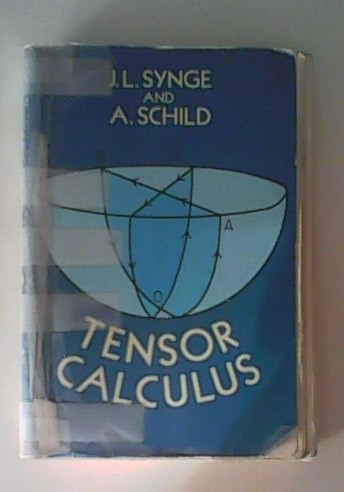
\includegraphics[width=10cm]{./images/zebook.jpg}
  \caption{My copy, falling apart...}
  \label{fig:test}
\end{figure}

\section*{Remarks and warnings}
You're welcome to use these notes, but they may contain errors, so proceed with caution : I graduated in 1979, went straight in the industry (where I didn't have to use fancy maths), and picked mathematics and physics again after I retired, so my mathematics got rusty  for sure. If you do find an error, typo's , I'd be happy to receive bug reports, suggestions, and the like, through Github.
An overview of the material covered in the book can be found in the separate document "Synge overview.pdf".

\section*{Some notation conventions}

\begin{center}
\begin{tabular}{ l l }
$\dagger$& means that the exercise has only been solved partially or contains i.m.o. a doubtful step\\\\
$\dagger \dagger$& means that the exercise has not been  solved as it should.\\\\
$\blacklozenge$&end of an exercise or proof.\\\\
$\lozenge$&end of Lemma or sub-task of an exercise.\\\\
&\textbf{As a rule, I followed the notation used in the book,}\\ &\textbf{except some which where easier to type in Latex.}\\\\
$\partial_r $ &$\equiv \pdv{}{x^r}$  \\\\
$\partial^2_{rs}$  &$\equiv \frac{\partial^2}{\partial x^r \partial x^s}$ \\\\
$\Gamma^r_{mn} $&$\equiv 
\begin{Bmatrix}
r\\
m n\\
\end{Bmatrix}\quad$  Christoffel symbol of the second kind\\\\
\end{tabular}
\end{center}

\tableofcontents
\listoffigures
\chapter{Spaces and Tensors}
\pagebreak[4]

\section{p5-exercise}

\begin{tcolorbox}

The parametric equations of a hypersurface in $V_n$ are
\begin{align*} 
\ &x^1 = a \cos(u^1)\\
\ &x^2 = a \sin(u^1)\cos(u^2)\\
\ &x^3 = a \sin(u^1)\sin(u^2)\cos(u^3)\\
\vdots\\
\ &x^{N-1} = a \sin(u^1)\sin(u^2)\sin(u^3)\dots\sin(u^{N-2})\cos(u^{N-1})\\
\ &x^{N} = a \sin(u^1)\sin(u^2)\sin(u^3)\dots\sin(u^{N-2})\sin(u^{N-1})\\
\end{align*}
where a is a constant. Find the single equation of the hyperspace in the form 1.103.

\end{tcolorbox}

We have:
\begin{align*}
\ (x^N)^2 + (x^{N-1})^2 &= a^2\prod_{i=1}^{N-2}\sin^2(u^i)(\cos^2(u^{N-1})+\sin^2(u^{N-1}))  \\
\ &= a^2\prod_{i=1}^{N-2}\sin^2(u^i)\\
\ &= a^2\prod_{i=1}^{N-3}\sin^2(u^i)\sin^2(u^{N-2})\\
\ &= a^2\prod_{i=1}^{N-3}\sin^2(u^i)(1-\cos^2(u^{N-2})\\
\ &= a^2\prod_{i=1}^{N-3}\sin^2(u^i) - a^2\prod_{i=1}^{N-3}\sin^2(u^i)\cos^2(u^{N-2})\\
\ &= a^2\prod_{i=1}^{N-3}\sin^2(u^i) - (x^{N-2})^2\\
\end{align*}
giving
$$(x^N)^2 + (x^{N-1})^2 + (x^{N-2})^2 = a^2\prod_{i=1}^{N-3}\sin^2(u^i)$$
In general, by recursion
$$\sum_{i=0}^k(x^{N-i})^2 = a^2\prod_{i=1}^{N-k-1}\sin^2(u^i)     \quad (k \leq N-2)$$
be k = N - 2 (N - k - 1 = 1) and in the left term put j = N - i (j goes from 2 to N), we get
\begin{align*}
\sum_{j=2}^N(x^{j})^2 &= a^2\prod_{i=1}^{1}\sin^2(u^i)\\
\ &= a^2(1-\cos^2(u^1))\\
\ &= a^2 - (x^1)^2\\
\end{align*}
and thus the equation of the hyperspace is given by
\begin{LARGE}
\textbf{
$$\sum_{j=1}^N(x^{j})^2 - a^2 = 0$$
}
\end{LARGE}
\begin{tcolorbox}

Determine whether the points $(\frac{1}{2}a,0,0,... 0)$, $(0,0,...,0, 2a)$ lie on the same or opposite sides of the hyperspace.
\end{tcolorbox}
For $(\frac{1}{2}a,0,0,... 0)$ we have $\sum_{j=1}^N(x^{j})^2 - a^2 = -\frac{3a^2}{4} < 0$ and for 
$(0,0,...,0, 2a)$ \\we have $\sum_{j=1}^N(x^{j})^2 - a^2 = \frac{3a^2}{4} > 0$.\\
So the points lie on opposite sides of the hyperplane.
$$\blacklozenge$$
\pagebreak[4]

\section{p6-exercise}

\begin{tcolorbox}

Let $U_2$ and $W_2$ be subspaces of $V_N$. Show that if N = 3  they will in general intersect in a curve; if N = 4 they will in general intersect in a finite number of points; and if $N > 4$ they will not in general intersect at all.
\end{tcolorbox}

We have (see 1.102 page 5):
$\quad x^r = f^r(u^1, u^2,..., u^M) \quad (r = 1, 2, ...,N)$

Case N=3: \\

For $U_2$ we have:
$$x^r = \phi^r(u^1, u^2) \quad (r = 1, 2, 3)$$

For $W_2$ we have:
$$x^r = \psi^r(v^1, v^2) \quad (r = 1, 2, 3)$$

The intersect of the two hyperplanes is given by the N equations:

$$\phi^r(u^1, u^2) = \psi^r(v^1, v^2) \quad (r = 1, 2, 3)$$

So we have 3 equations in 4 unknown $u^1,u^2, v^1, v^2$ and can choose (fix) one e.g. $u^1$ and solve the set of equations  for $u^2, v^1, v^2$ giving 
$$x^r = \theta^r(u^1) \quad (r = 1, 2, 3)$$
This is an equation of a curve in space (1 parameter equation)\\
Case N=4: \\
Using the same reasoning as with N=3, we get 4 equations for 4 unknown $u^1,u^2, v^1, v^2$.\\
Provided that the set of equation does not degenerate, these 4 equations will determine $u^1,u^2, v^1, v^2$ without any degree of freedom. So we get  points as solutions. This solution does not to be unique, e.g. if the $\phi^r(u^1, u^2)$ are quadratic form, then the solutions 
$$(u^1,u^2, v^1, v^2)$$
$$(-u^1,u^2, v^1, v^2)$$
$$ (u^1,-u^2, v^1, v^2)$$
$$ (-u^1,-u^2, v^1, v^2)$$
are possible.\\
Case N=5: 
There are more equations than variables. If the equations are not linear dependent, no solutions will be found.
$$\blacklozenge$$
\pagebreak[4]
\section{p8-exercise}

\begin{tcolorbox}
Show that $(a_{rst}+a_{str}+a_{srt})x^rx^sx^t = 3a_{rst}x^rx^sx^t$
\end{tcolorbox}
%\setcounter {equation} {1} %sets the counter to have the specified
$(a_{rst}+a_{str}+a_{srt})x^rx^sx^t = a_{rst}x^rx^sx^t+a_{rts}x^rx^sx^t+a_{srt}x^rx^sx^t\quad$
so by just renaming the dummy indices e.g. for the second term  $r \mapsto s\quad$, $s \mapsto t\quad$ and $t \mapsto r\quad$ we get the desired result.
$$\blacklozenge$$
\pagebreak[4]

\section{p8-exercise}

\begin{tcolorbox}
If $\phi = a_{rs}x^rx^s$, show that
$$\pdv{\phi}{x^{r}} = (a_{rs}+a_{sr})x^s \quad\text{,}\quad\pdv{\phi}{x^{r}}{x^{s}} = a_{rs}+a_{sr}$$
Simplify these expressions in the case where $a^{rs} = a^{sr}$
\end{tcolorbox}
We have 
\begin{align} 
\pdv{\phi}{x^{t}} &= \pdv{a_{rs}}{x^{t}}x^{r}x^{s}+a_{rs}\pdv{x^{r}}{x^{t}}x^{s}+a_{rs}x^{r}\pdv{x^{s}}{x^{t}}\\
&= \pdv{a_{rs}}{x^{t}}x^{r}x^{s}+a_{rs}\delta_t^rx^{s}+a_{rs}x^{r}\delta^s_t\\
&= \pdv{a_{rs}}{x^{t}}x^{r}x^{s}+a_{ts}x^{s}+a_{rt}x^{r}\\
&= \pdv{a_{rs}}{x^{t}}x^{r}x^{s}+a_{ts}x^{s}+a_{st}x^{s}\quad\text{(rename dummy variable in third term)}\\
&= \pdv{a_{rs}}{x^{t}}x^{r}x^{s}+(a_{ts}+a_{st})x^{s}
\end{align}
Replace $x^t$ by $x^r$, we get
\begin{align}
\pdv{\phi}{x^{r}}  =\pdv{a_{rs}}{x^{r}}x^{r}x^{s}+(a_{rs}+a_{sr})x^{s}
\end{align}
So the asked expression is only true if $a_{rs}$ is not a function of the $x^{s}$.
Assuming that $a_{rs}$ is not a function of the $x^{s}$, take the partial derivative of (6) with respect to $x^{t}$, we get
\begin{align} 
\pdv{\phi}{x^{r}}{x^{t}} &= (a_{rs}+a_{sr})\pdv{x^{s}}{x^{t}}\\
&=(a_{rs}+a_{sr})\delta^{s}_{t}\\
&=(a_{rt}+a_{tr})
\end{align}
Replace $x^t$ by $x^s$, and we get the proposed expression.
$$\blacklozenge$$
\pagebreak[4]

\section{p8-clarification on expression 1.210}

\begin{tcolorbox}
$$\pdv{x^{'q}}{x^{p}}{x^{s}}+\pdv{x^{r}}{x^{'m}}{x^{'n}}\pdv{x^{'m}}{x^{p}}\pdv{x^{'n}}{x^{s}}\pdv{x^{'q}}{x^{r}} = 0 $$
\end{tcolorbox}
From 1.209:
\begin{gather} 
\pdv{x^r}{x^{'m}}{x^{'n}}\pdv{x^{'m}}{x^{p}}\pdv{x^{'n}}{x^{s}}+\pdv{x^r}{x^{'n}}\pdv{x^{'n}}{x^p}{x^{s}} = 0
\end{gather}
 multiply (1)  with $\quad\pdv{x^{'q}}{x^{r}}$
\begin{gather} 
\pdv{x^r}{x^{'m}}{x^{'n}}\pdv{x^{'m}}{x^{p}}\pdv{x^{'n}}{x^{s}}\pdv{x^{'q}}{x^{r}}+\pdv{x^r}{x^{'n}}\pdv{x^{'n}}{x^p}{x^{s}}\pdv{x^{'q}}{x^{r}} = 0\\
\Leftrightarrow\pdv{x^r}{x^{'n}}\pdv{x^{'n}}{x^p}{x^{s}}\pdv{x^{'q}}{x^{r}}+ \pdv{x^r}{x^{'m}}{x^{'n}}\pdv{x^{'m}}{x^{p}}\pdv{x^{'n}}{x^{s}}\pdv{x^{'q}}{x^{r}}= 0
\end{gather}
\begin{gather} 
\text{\centering in the first term we get\quad\quad}\quad \pdv{x^{'q}}{x^{r}}\pdv{x^r}{x^{'n}} = \pdv{x^{'q}}{x^{'n}} = \delta_n^q
\end{gather}
(3) becomes
\begin{gather} 
\pdv{x^{'n}}{x^p}{x^{s}}\delta_n^q + \pdv{x^r}{x^{'m}}{x^{'n}}\pdv{x^{'m}}{x^{p}}\pdv{x^{'n}}{x^{s}}\pdv{x^{'q}}{x^{r}}=  0\\
\Leftrightarrow\pdv{x^{'q}}{x^p}{x^{s}} + \pdv{x^r}{x^{'m}}{x^{'n}}\pdv{x^{'m}}{x^{p}}\pdv{x^{'n}}{x^{s}}\pdv{x^{'q}}{x^{r}}= 0
\end{gather} 
$$\blacklozenge$$
\pagebreak[4]



\section{p9-exercise}

\begin{tcolorbox}
If $A_s^r$ are the elements of a determinant A, and $B_s^r$ the elements of a determinant B, show that the element of the product determinant is $A_n^rB^n_s$. Hence show that the product of the two jacobians
$$J =\Bigg|\pdv{x^{r}}{x^{'s}}\Bigg|\text{,}\quad J^{'} = \Bigg|\pdv{x^{'r}}{x^{s}}\Bigg|$$
is unity.
\end{tcolorbox}
Remark: Some nitpick about the formulation: $A_s^r$ are not the elements of a determinant A, but elements of the matrix A which gives $\det{A}$ provided that A is square (which is not explicitly mentioned.). The same remark for B and $A_n^rB^n_s$.\\
Be $A^i_k $ the elements of matrix A and $B^k_j $ the elements of matrix B and C = A.B the resulting matrix of the multiplication of A and B, then
$$C^i_j  = A^i_kB^k_j $$
are the elements of matrix C.
Now, put $A^i_k =\pdv{x^{i}}{x^{'k}} \quad$ and $B^k_j =\pdv{x^{'k}}{x^{j}} \quad$ then,
\begin{align}
C^{i}_{j}  &= A^{i}_{k}B^{k}_{j} \\
&=\pdv{x^{i}}{x^{'k}}\pdv{x^{'k}}{x^{j}}\\
&= \delta^{i}_{k}
\end{align}
So $C = JJ^{'}\quad$becomes the unity matrix. 
$$\blacklozenge$$
\pagebreak[4]

\section{p11-exercise}

\begin{tcolorbox}
Show that a finite contravariant vector determines the ratios of the components of an infinitesimal displacement. (Consider the transformation of the equation $dx^r=\theta T^r$, where $\theta$ is an arbitrary factor which does not change under the transformation. Alternatively, show that the equations $T^{r} dx^{s}-T^{s} x^{r} = 0$ remain true when we transform the coordinates.)

\end{tcolorbox}
Be $T^{q}$ a contravariant vector.
\begin{align}
T^{'q}=T^{r} \pdv{x^{'q}}{x^r}\quad\text{(by definition)}
\end{align}
Be  $\theta$ a small infinitesimal factor invariant for a coordinate transformation,  define \\
\begin{align}
\ dx^{r} = \theta T^{r} \\
\end{align}
then
\begin{align}
\dv{x^r}{x^s} = \frac{\theta T^r}{\theta T^s}\\
\Leftrightarrow T^s dx^r - T^r dx^s = 0
\end{align}
Alternatively, multiply (5) with $\partial_{x^r}{x^{'q}}$, then
\begin{align}
\pdv{x^{'q}}{x^r} dx^r T^s   -  \pdv{x^{'q}}{x^r}dx^s T^r &= 0\\
\Leftrightarrow \pdv{x^{'q}}{x^r} dx^r T^s   -  dx^s T^{'q} &= 0 \quad \text{(use (1) in the second term)}\\
\Leftrightarrow dx^{'q} T^s   -  dx^s T^{'q} &= 0 \\
\end{align}
Multiply (8) with $\partial_{x^s}{x^{'p}}$, then
\begin{align}
\ &dx^{'q} T^s \partial_{x^s}{x^{'p}}  -  dx^s T^{'q}\partial_{x^s}{x^{'p}} = 0 \\
\Leftrightarrow \quad &T^{'p} dx^q   -   T^{'q} dx^{'p} = 0 \quad \text{(use (1) in the first term)}
\end{align}
and thus 
$$\dv{x^{'q}}{x^{'p}} = \frac{T^{'q}}{T^{'p}}$$

$$\blacklozenge$$
\pagebreak[4]


\section{p12-exercise}

\begin{tcolorbox}
Write down the equation of transformation, analogous to 1.305, of a contravariant tensor of the third order. Solve the equation so as to express the unprimed components in terms of the primed components.

\end{tcolorbox}
Be 
\begin{align}
T^{'uvw}=T^{rst} \pdv{x^{'u}}{x^r}\pdv{x^{'v}}{x^s}\pdv{x^{'w}}{x^t}\quad\text{(by definition)}
\end{align}
a contravariant vector.\\
Multiply (1) by $\pdv{x^{n}}{x^{'u}}$
\begin{align}
\ T^{'uvw}\pdv{x^{n}}{x^{'u}}&= T^{rst} \pdv{x^{'u}}{x^r}\pdv{x^{n}}{x^{'u}}\pdv{x^{'v}}{x^s}\pdv{x^{'w}}{x^t}\\
\Leftrightarrow  T^{'uvw}\pdv{x^{n}}{x^{'u}}&= T^{rst} \delta^{n}_{r}\pdv{x^{'v}}{x^s}\pdv{x^{'w}}{x^t}\\
\Leftrightarrow  T^{'uvw}\pdv{x^{n}}{x^{'u}}&= T^{nst} \pdv{x^{'v}}{x^s}\pdv{x^{'w}}{x^t}
\end{align}
Multiply (4) by $\pdv{x^{m}}{x^{'v}}$
\begin{align}
\ T^{'uvw}\pdv{x^{n}}{x^{'u}}\pdv{x^{m}}{x^{'v}} &= T^{nst} \pdv{x^{'v}}{x^s}\pdv{x^{m}}{x^{'v}}\pdv{x^{'w}}{x^t}\\
\Leftrightarrow  \ T^{'uvw}\pdv{x^{n}}{x^{'u}}\pdv{x^{m}}{x^{'v}} &= T^{nst} \delta_{s}^{m}\pdv{x^{'w}}{x^t}\\
\Leftrightarrow  \ T^{'uvw}\pdv{x^{n}}{x^{'u}}\pdv{x^{m}}{x^{'v}} &= T^{nmt} \pdv{x^{'w}}{x^t}
\end{align}
Multiply (7) by $\pdv{x^{p}}{x^{'w}}$
\begin{align}
\ T^{'uvw}\pdv{x^{n}}{x^{'u}}\pdv{x^{m}}{x^{'v}}\pdv{x^{p}}{x^{'w}} &= T^{nmt} \pdv{x^{'w}}{x^t}\pdv{x^{p}}{x^{'w}}\\
\Leftrightarrow \ T^{'uvw}\pdv{x^{n}}{x^{'u}}\pdv{x^{m}}{x^{'v}}\pdv{x^{p}}{x^{'w}} &= T^{nmt} \delta^{p}_{t}\\
\Leftrightarrow  \ T^{'uvw}\pdv{x^{n}}{x^{'u}}\pdv{x^{m}}{x^{'v}}\pdv{x^{p}}{x^{'w}} &= T^{nmp} 
\end{align}
Giving
$$T^{nmp} =  T^{'uvw}\pdv{x^{n}}{x^{'u}}\pdv{x^{m}}{x^{'v}}\pdv{x^{p}}{x^{'w}} $$

$$\blacklozenge$$
\pagebreak[4]

\section{p14-exercise}

\begin{tcolorbox}
For a transformation from on set of rectangular Cartesian coordinates to another in Euclidean 3-space, show that the law of transformation of a contravariant vector is precisely the same as that of a covariant vector. Can this statements be extended to cover tensor of higher orders?
\end{tcolorbox}
We have to prove that, given that, $$T^{'i}= T^{j} \pdv{x^{'i}}{x^j} \quad T^{'}_{i}= T_{j} \pdv{x^{j}}{x^{'i}}$$ that also
\begin{align}
\ T^{'i}= T^{j} \pdv{x^{j}}{x^{'i}} \quad T^{'}_{i}&= T_{j}\pdv{x^{'i}}{x^j} \\
\Leftrightarrow \pdv{x^{j}}{x^{'i}} &= \pdv{x^{'i}}{x^j} 
\end{align}
Be
\begin{align}
\hat{e^{'i}} = g^i_k\hat{e^{k}}\quad\text{and } \hat{e^{i}} = h^i_k\hat{e^{'k}}
\end{align}
the transformation rules from one set of (rectangular Cartesian) basis vectors to another set of  (rectangular Cartesian) basis vectors.
Then,
\begin{align}
\langle \hat{e^{'i}},\hat{e^{'j}} \rangle = \langle g^i_k\hat{e^{k}},g^j_k\hat{e^{k}} \rangle &\text{ and } \langle \hat{e^{i}},\hat{e^{j}} \rangle = \langle h^i_k\hat{e^{'k}},h^j_k\hat{e^{'k}} \rangle\\
\Leftrightarrow \delta^p_j = g^p_k g^j_k &\text{ and } \delta^p_j = h^p_k h^j_k \\
\end{align}
Be $\vec{v}$ a random vector in the Euclidean space,
\begin{align}
\vec{v} = x^j\hat{e^{j}} = x^{'j}\hat{e^{'j}}
\end{align}
then
\begin{align}
\text{(3) } \Rightarrow x^j\hat{e^{j}} = x^{j}h^j_k\hat{e^{'k}}&\text{ and }x^{'j}\hat{e^{'j}} = x^{'j}g^j_k\hat{e^{k}}\\
\Rightarrow x^{'j} = x^{m}h^m_j  &\text{ and }x^m = x^{'j}g^j_m\\
\Rightarrow x^{'j} = x^{'i}g^i_m h^m_j&\text{ and } x^m = x^{k}h^k_j g^j_m \\
\Rightarrow \delta^p_j =g^p_k h^k_j &\text{ and } \delta^p_j =g^k_j h^p_k\\
\text{(5) } \Rightarrow g^p_k g^j_k=g^p_k h^k_j &\text{ and } h^p_k h^j_k=g^k_j h^p_k\\
 \Rightarrow g^j_k =  h^k_j &\text{ and }h^j_k =  g^k_j
\end{align}
From (9)
\begin{align}
\ x^{j} = x^{'m} g^m_j &\text{ and } x^{'k} = x^{n} h^n_k\\
\Rightarrow \pdv{x^{'k}}{x^j} = \pdv{x^{n}}{x^j} h^n_k  &\text{ and } \pdv{x^{j}}{x^{'k}} = \pdv{x^{'m}}{x^{'k}}g^m_j\\
\Leftrightarrow \pdv{x^{'k}}{x^j} = \delta^n_j h^n_k  &\text{ and } \pdv{x^{j}}{x^{'k}} = \delta^m_k g^m_j\\
\Leftrightarrow \pdv{x^{'k}}{x^j} = h^j_k  &\text{ and } \pdv{x^{j}}{x^{'k}} = g^k_j\\
\text{(13) }\Rightarrow \pdv{x^{'k}}{x^j} &= \pdv{x^{j}}{x^{'k}}
\end{align}
So (13) matches (2), proving the assertion.\\\\
Can this statements be extended to cover tensor of higher orders?
Consider
$$T^{'i,j,\dots ,n}= T^{r,s,\dots w} \pdv{x^{'i}}{x^{r}}\pdv{x^{'j}}{x^{s}}\dots \pdv{x^{'n}}{x^{w}} \text{ and } T^{r,s,\dots w}= T^{'i,j,\dots ,n} \pdv{x^{r}}{x^{'i}}\pdv{x^{s}}{x^{'j}}\dots \pdv{x^{w}}{x^{'n}}$$
Using the same reasoning as in (1) to (2) we need
$$\pdv{x^{'i}}{x^{r}}\pdv{x^{'j}}{x^{s}}\dots \pdv{x^{'n}}{x^{w}} =\pdv{x^{r}}{x^{'i}}\pdv{x^{s}}{x^{'j}}\dots \pdv{x^{w}}{x^{'n}}$$
As the conclusion (18) is independent of the order of the tensor, it is obvious that the above equality yields. Hence, the answer is YES.

$$\blacklozenge$$
\pagebreak[4]

\section{p16-exercise}

\begin{tcolorbox}
In a space of 4 dimensions, the tensor $A_{rst}$ is skew-symmetric in the last pair of suffixes. Show that only 24 of the 64 components may be chosen arbitrarily. If the further condition
$A_{rst} + A_{str}+A_{trs} =0$
is imposed, show that that only 20 components may be chosen arbitrarily.

\end{tcolorbox}
We have, as A is skew-symmetric in the last pair of suffixes
$$A_{rst} = -A_{rts}  \Rightarrow s=t \text{: } A_{rst} = 0 $$
So, for each r (4 possible choices as N = 4) we have 4x4/2 - 4 = 6 degrees of freedom. [we have the term 4x4/2  as the tensor is (skew-)symmetric, e.g. once we choose element $a_{12}$, then $a_{21}$ is also known. The term -4 takes into account the diagonal element which are 0 and thus cannot be chosen.]\\
So, we have 4x6 = 24 degrees of freedom.\\
What about the supplementary constraint $A_{rst} + A_{str}+A_{trs} =0 $       :\\
Consider the two possible excluding cases:\\

i) $r=s\neq t \text{ (}\Leftrightarrow r=t\neq s \text{)}$\\
This case gives - without the additional constraint (1) -  4x(4x3/2-4) = 8 degrees of freedom.
Does the constraint (1) reduces this degree of freedom?\\
We have, 
\begin{align}
\ A_{rst} + A_{str}+A_{trs} =0\\
\Rightarrow \underbrace{A_{rrt} + A_{rtr}}_\text{= 0 (non-diagonal terms)} + \underbrace{A_{trr}}_\text{= 0 (diagonal terms)} =0
\end{align}
So, no additional constraints are added by (1) to the restriction i) and the DOF remains 8.\\

ii) $t \neq r\neq s\neq t$\\
This case means that we have to choose a set of 3 elements out of 4 elements without repetition. This a \textit{variation} of 3 elements out of 4.
$$V^n_{k} = \frac{n!}{(n-k)!} \text{ giving } V^4_{3} = \frac{4!}{(4-3)!} = 24 $$
The constraint (1) gives us 24 equations but as  $A_{rst} = -A_{rts}$ only 12 equations have to be considered. So, with the  additional constraints the DOF becomes 24-12 = 12.\\
As i) and ii) are independent and excluding events we can add the DOF of both events and we get 8+12 = 20 DOF.

$$\blacklozenge$$
\pagebreak[4]

\section{p16-exercise}

\begin{tcolorbox}
If $A^{rs}$ is skew-symmetric and $B_{rs}$ is symmetric, prove that $A^{rs}B_{rs} = 0$. Hence show that the quadratic form $a_{ij}x^ix^j$ is unchanged if $a_{ij}$ is replaced by its symmetric part.
\end{tcolorbox}
We can split the summation $A^{rs}B_{rs}$ in three subsummations:
\begin{align}
\ A^{rs}B_{rs}  = &A^{rs}B_{rs} \vert_{r=s} \\
\ + &A^{rs}B_{rs}\vert_{r>s} \\
\ + &A^{rs}B_{rs}\vert_{r<s}
\end{align}
We have:\\
(1) = 0 as $A^{kk} = 0$ (skew-symmetric)\\
(2)+(3) = $A^{rs}B_{rs}\vert_{r>s} \ + A^{rs}B_{rs}\vert_{r<s}$\\
As $A^{rs} = -A^{sr}$ and $B^{rs} = B^{sr}$ we can write (2)+(3) as :
$$A^{rs}B_{rs}\vert_{r>s} \ + (-A^{sr})B_{sr}\vert_{r>s} = 0$$
So, $A^{rs}B_{rs} = 0$\\\\
Consider the quadratic form $\phi = a_{ij}x^ix^j$\\
Be $A_{ij} = (a_{ij})$ and $B_{ij} = (x^ix^j)$, then it is obvious that $B_{ij}$ is symmetric and that $C_{ij} = -A_{ij}$ is the form where $-a_{ij}$ is replaced by its symmetric part (skew-symmetric).
Hence $\phi = a_{ij}x^ix^j =a_{ij}b^{ij}= 0$ and so is $\phi = c_{ij}b^{ij}= 0$ 

$$\blacklozenge$$
\pagebreak[4]

\section{p18-exercise}

\begin{tcolorbox}
What are the values (in a space of N dimensions) of the folllowing contractions formed from the Kronecker delta?
$$\delta^{m}_{m},  \delta^{m}_{n} \delta^{n}_{m},  \delta^{m}_{n} \delta^{n}_{r} \delta^{r}_{m}$$
\end{tcolorbox}
\begin{align}
\delta^{m}_{m} = N\\
\delta^{m}_{n} \delta^{n}_{m} = \delta^{m}_{m} = N\\
\delta^{m}_{n} \delta^{n}_{r} \delta^{r}_{m} = \delta^{m}_{n} \delta^{n}_{m} = \delta^{m}_{m} = N
\end{align}
$$\blacklozenge$$
\pagebreak[4]

\section{p19-exercise}
\begin{tcolorbox}
If $X^{r}$, $Y^{r}$ are arbitrary contravariant vectors and $a_{rs}X^{r}Y^{s}$ is an invariant, then $a_{rs}$ are the components of a covariant tensor of the second order. 
\end{tcolorbox}
We have to prove that
\begin{align}
\ a^{'}_{rs} = a_{ij}\pdv{x^{i}}{x^{'r}}\pdv{x^{j}}{x^{'s}} \text{ or } a^{}_{ij} = a^{'}_{rs}\pdv{x^{'r}}{x^{i}}\pdv{x^{'s}}{x^{j}}
\end{align}
$a_{rs}X^{r}Y^{s}$ is an invariant, means
\begin{align}
\ a^{'}_{rs}X^{'r}Y^{'s} = a_{rs}X^{r}Y^{s}
\end{align}
As $X^{r}$, $Y^{r}$ are arbitrary contravariant vectors, we have
\begin{align}
\ X^{'r} = X^{i}\pdv{x^{'r}}{x^{i}} \text{   and  } Y^{'s} = Y^{j}\pdv{x^{'s}}{x^{j}}
\end{align}
(3) in (2) gives
\begin{align}
\ a^{'}_{rs}X^{i}\pdv{x^{'r}}{x^{i}}Y^{j}\pdv{x^{'s}}{x^{j}} = a_{rs}X^{r}Y^{s}\\
\Leftrightarrow a^{'}_{rs}\pdv{x^{'r}}{x^{i}}\pdv{x^{'s}}{x^{j}}X^{i}Y^{j} = a_{ij}X^{i}Y^{j}\\
\Leftrightarrow (a^{'}_{rs}\pdv{x^{'r}}{x^{i}}\pdv{x^{'s}}{x^{j}} - a_{ij})X^{i}Y^{j} = 0
\end{align}
As $X^{r}$, $Y^{r}$ are arbitrary contravariant vectors, we conclude that 
\begin{align}
\ a^{'}_{rs}\pdv{x^{'r}}{x^{i}}\pdv{x^{'s}}{x^{j}} - a_{ij} = 0\\
\Leftrightarrow a_{ij} =  a^{'}_{rs}\pdv{x^{'r}}{x^{i}}\pdv{x^{'s}} {x^{j}}
\end{align}
(8) = (1): OK
$$\blacklozenge$$
\pagebreak[4]

\section{p19-exercise}
\begin{tcolorbox}
If $X_{rs}$ is an arbitrary covariant tensor of the second order, and $A^{mn}_{r }X_{mn}$ is a covariant vector, then $A^{mn}_{r }$ has the mixed tensor character indicated by the positions of its suffixes 
\end{tcolorbox}
We have to prove that
\begin{align}
\ A^{'vw}_{r} = A^{mn}_k\pdv{x^{k}}{x^{'r}}\pdv{x^{'v}}{x^{m}}\pdv{x^{'w}}{x^{n}} 
\end{align}
We have
\begin{align}
\ P_{r} =A^{mn}_{r }X_{mn}
\end{align}
is a covariant vector
\begin{align}
\Rightarrow P^{'}_{r} =A^{mn}_{k }X_{mn}\pdv{x^{k}}{x^{'r}}
\end{align}
but $X_{mn}$ is a covariant tensor
\begin{align}
\Rightarrow X_{mn} = X^{'}_{ps}\pdv{x^{'p}}{x^{m}}\pdv{x^{'s}}{x^{n}}
\end{align}
So (4) in (3) gives
\begin{align}
\ P^{'}_{r} =A^{mn}_{k }X^{'}_{ps}\pdv{x^{'p}}{x^{m}}\pdv{x^{'s}}{x^{n}}\pdv{x^{k}}{x^{'r}}\\
\Leftrightarrow P^{'}_{r} = \underbrace{A^{mn}_{k }\pdv{x^{'p}}{x^{m}}\pdv{x^{'s}}{x^{n}}\pdv{x^{k}}{x^{'r}}}_\text{(*)}X^{'}_{ps}
\end{align}
Putting (*) as $ A^{'ps}_{r }= A^{mn}_{k }\pdv{x^{'p}}{x^{m}}\pdv{x^{'s}}{x^{n}}\pdv{x^{k}}{x^{'r}}$ we see that (6) has the form (2) and that $A^{'ps}_{r }$ obeys the rule of a mixed tensor (1).
$$\blacklozenge$$
\pagebreak[4]

\section{p21-exercise}
\begin{tcolorbox}
If $A_{rs}$ is a skew-symmetric covariant tensor, prove that $B_{rst}$ defined as 
$$B_{rst} = \partial_{r}{A_{st}} + \partial_{s}{A_{tr}} +\partial_{t}{A_{rs}} $$ is a covariant tensor, and that it is skew-symmetric in all pairs of suffixes.
\end{tcolorbox}

We have $A_{rs}$ is a covariant tensor
\begin{align}
\ A_{ij} &= A_{\alpha\beta}\pdv{x^{\alpha}}{x^{i}}\pdv{x^{\beta}}{x^{j}}\\
\Rightarrow B_{rst} &= \partial_{r}{(A_{\alpha\beta}\pdv{x^{\alpha}}{x^{s}}\pdv{x^{\beta}}{x^{t}})} + \partial_{s}{(A_{\alpha\beta}\pdv{x^{\alpha}}{x^{t}}\pdv{x^{\beta}}{x^{r}})} +\partial_{t}{(A_{\alpha\beta}\pdv{x^{\alpha}}{x^{r}}\pdv{x^{\beta}}{x^{s}})}
\end{align}
Note that
\begin{align}
\partial_{k}{(A_{\alpha\beta}\pdv{x^{\alpha}}{x^{s}}\pdv{x^{\beta}}{x^{t}})} = 
\partial_{k}{(A_{\alpha\beta})}\pdv{x^{\alpha}}{x^{s}}\pdv{x^{\beta}}{x^{t}}+
\ A_{\alpha\beta}\partial_{k}{(\pdv{x^{\alpha}}{x^{s}})}\pdv{x^{\beta}}{x^{t}}+
\ A_{\alpha\beta}\pdv{x^{\alpha}}{x^{s}} \partial_{k}{(\pdv{x^{\beta}}{x^{t}})}\\
\end{align}
so, 
\begin{align}
\begin{array}{r c l}
\ B_{rst} = \partial_{r}{A_{\alpha\beta}}\pdv{x^{\alpha}}{x^{s}}\pdv{x^{\beta}}{x^{t}}+ \underbrace{A_{\alpha\beta}\partial_{r}{\pdv{x^{\alpha}}{x^{s}}}\pdv{x^{\beta}}{x^{t}}}_\text{*} +\underbrace{A_{\alpha\beta}\pdv{x^{\alpha}}{x^{s}}\partial_{r}{\pdv{x^{\beta}}{x^{t}}}}_\text{**}\\ +
\partial_{s}{A_{\alpha\beta}}\pdv{x^{\alpha}}{x^{t}}\pdv{x^{\beta}}{x^{r}}+\underbrace{A_{\alpha\beta}\partial_{s}{\pdv{x^{\alpha}}{x^{t}}}\pdv{x^{\beta}}{x^{r}}}_\text{***}+\underbrace{A_{\alpha\beta}\pdv{x^{\alpha}}{x^{t}}\partial_{s}{\pdv{x^{\beta}}{x^{r}}}}_\text{*}\\+
\partial_{t}{A_{\alpha\beta}}\pdv{x^{\alpha}}{x^{r}}\pdv{x^{\beta}}{x^{s}}+A_{\alpha\beta}\underbrace{\partial_{t}{\pdv{x^{\alpha}}{x^{r}}}\pdv{x^{\beta}}{x^{s}}}_\text{**}+\underbrace{A_{\alpha\beta}\pdv{x^{\alpha}}{x^{r}}\partial_{t}{\pdv{x^{\beta}}{x^{s}}}}_\text{***}
\end{array}
\end{align}
In (5) consider the two terms with (*) 
\begin{align}
\ T &= A_{\alpha\beta}\partial_{r}{\pdv{x^{\alpha}}{x^{s}}}\pdv{x^{\beta}}{x^{t}}+ A_{\alpha\beta}\pdv{x^{\alpha}}{x^{t}}\partial_{s}{\pdv{x^{\beta}}{x^{r}}}\\
& = A_{\alpha\beta}\pdv{x^{\alpha}}{x^{s}}{x^{r}}\pdv{x^{\beta}}{x^{t}}+ A_{\alpha\beta}\pdv{x^{\alpha}}{x^{t}}\pdv{x^{\beta}}{x^{r}}{x^{s}}\\
& = A_{\alpha\beta}\pdv{x^{\alpha}}{x^{s}}{x^{r}}\pdv{x^{\beta}}{x^{t}}+ A_{\beta\alpha}\pdv{x^{\beta}}{x^{t}}\pdv{x^{\alpha}}{x^{r}}{x^{s}} \text{ (by renaming dummy variables)}
\end{align}
As $A_{ij} = - A_{ji}$ (skew-symmetric tensor), we get $T=0$. The same yields for the (**) and (***) terms. So, $B_{rst}$ reduces to
\begin{align}
\ B_{rst} = \partial_{r}{A_{\alpha\beta}}\pdv{x^{\alpha}}{x^{s}}\pdv{x^{\beta}}{x^{t}}+ 
\partial_{s}{A_{\alpha\beta}}\pdv{x^{\alpha}}{x^{t}}\pdv{x^{\beta}}{x^{r}}+
\partial_{t}{A_{\alpha\beta}}\pdv{x^{\alpha}}{x^{r}}\pdv{x^{\beta}}{x^{s}}\\
\Leftrightarrow \ B_{rst} = \pdv{A_{\alpha\beta}}{x^{\gamma}}\pdv{x^{\gamma}}{x^{r}}\pdv{x^{\alpha}}{x^{s}}\pdv{x^{\beta}}{x^{t}}+ 
\pdv{A_{\alpha\beta}}{x^{\gamma}}\pdv{x^{\gamma}}{x^{s}}\pdv{x^{\alpha}}{x^{t}}\pdv{x^{\beta}}{x^{r}}+
\pdv{A_{\alpha\beta}}{x^{\gamma}}\pdv{x^{\gamma}}{x^{t}}\pdv{x^{\alpha}}{x^{r}}\pdv{x^{\beta}}{x^{s}}
\end{align}
By adequate renaming of the dummy variable in the 3 terms:
$$  \left[ {\begin{array}{c}
    1^{st} term \\
    2^{nd} term  \\
    3^{rd} term  
  \end{array} } \right]
\longrightarrow
  \left[ {\begin{array}{ccc}
    \gamma \to \alpha & \alpha \to \beta & \beta \to \gamma \\
    \beta \to \alpha & \gamma \to \beta & \alpha \to \gamma \\
    \alpha \to \alpha & \beta \to \beta & \gamma \to \gamma 
  \end{array} } \right]
$$
we get
\begin{align}
\ B_{rst} = (\pdv{A_{\beta\gamma}}{x^{\alpha}}+\pdv{A_{\gamma\alpha}}{x^{\beta}}+\pdv{A_{\alpha\beta}}{x^{\gamma}})\pdv{x^{\alpha}}{x^{r}}\pdv{x^{\beta}}{x^{s}}\pdv{x^{\gamma}}{x^{t}}\\
\Leftrightarrow  B_{rst} = (\underbrace{\partial_{\alpha}{A_{\beta\gamma}}+\partial_{\beta}{A_{\gamma\alpha}}+\partial_{\gamma}{A_{\alpha\beta}}}_\text{(****)})\pdv{x^{\alpha}}{x^{r}}\pdv{x^{\beta}}{x^{s}}\pdv{x^{\gamma}}{x^{t}}
\end{align}
The expression (****) has exactly the required form $B_{rst} = \partial_{r}{A_{st}} + \partial_{s}{A_{tr}} +\partial_{t}{A_{rs}} $ and is transformed (12) according the rules of a covariant tensor.\\
Let's prove now that it is skew-symmetric in all pairs of suffixes.
We have to consider the following permutations
$$  \left[ {\begin{array}{c}
    rst \\
    rts\\
    srt  \\
    str\\  
    trs \\
    tsr
  \end{array} } \right]$$
  
E.g. $srt$
\begin{align}
\ B_{rts} &= \partial_{r}{A_{ts}}+\partial_{t}{A_{sr}}+\partial_{s}{A_{rt}}\\
&= -\partial_{r}{A_{st}}-\partial_{t}{A_{rs}}-\partial_{s}{A_{tr}}\\
&= - B_{rst}
\end{align}
The same calculations can be done for the other permutations.
$$\blacklozenge$$
\pagebreak[4]

\section{p23-exercise 1.}
\begin{tcolorbox}
In a $V_{4}$ there are two 2-spaces with equations
$$x^r = f^r(u^1,u^2)\text{, }x^r = g^r(u^3,u^4) $$
Prove that if these 2-spaces have a curve of intersection, then the determinal equation
$$\left|\pdv{x^r}{u^s}\right| = 0$$
is satisfied along the curve.
\end{tcolorbox}
Having a curve means that one of the parameters $u^i$ can be freely chosen while the other 3 are determined by the chosen parameter.\\
We have,
\begin{align}
\left|\pdv{x^r}{u^s}\right| = \left| {\begin{array}{cccc}
    \pdv{x^1}{u^1} & \pdv{x^1}{u^2} & \pdv{x^1}{u^3} & \pdv{x^1}{u^4}\\
    \vdots & \vdots & \vdots & \vdots\\
    \pdv{x^4}{u^1} & \pdv{x^4}{u^2} & \pdv{x^4}{u^3} & \pdv{x^4}{u^4}\\
  \end{array} } \right|
\end{align}
Suppose we choose $u^4$ as parameter.
This means $u^i = \phi^i(u^4)$ for i=1,2,3 and thus we can write
\begin{align}
\pdv{x^i}{u^4} &= \pdv{x^i}{u^j}\dv{\phi^j}{u^4}+ \pdv{x^i}{u^4}\quad\text{ with j=1,2,3} \quad\text{  i = 1,2,3,4}\\
&\Rightarrow \pdv{x^i}{u^j}\dv{\phi^j}{u^4} = 0
\end{align}
This means that in (1) the three first columns a not linearly independent and thus have   $\left|\pdv{x^r}{u^s}\right| = 0$

$$\blacklozenge$$
\pagebreak[4]

\section{p23-exercise 2.}
\begin{tcolorbox}
In Euclidean space of three dimensions, write down the equations of transformation between rectangular Cartesian coordinates x, y, z and spherical polar coordinates $r$,$\theta$,$\phi$.\\
Find the Jacobian of the transformation. Where is it zero or infinite?
\end{tcolorbox}

\begin{figure}[h]
\centering
\begin{minipage}[t]{.6\textwidth}
%\centering
\vspace{0pt}
\tdplotsetmaincoords{60}{120}
\begin{tikzpicture}
	[scale=6,
		tdplot_main_coords,
		axis/.style={->,black,thick},
		vector/.style={-stealth,black, thick},
		vector guide/.style={dashed,black,thick},
		angle/.style={black,thick}]

	%standard tikz coordinate definition using x, y, z coords
	\coordinate (O) at (0,0,0);
	
	%tikz-3dplot coordinate definition using r, theta, phi coords
	\tdplotsetcoord{P}{.8}{55}{60}
	
	%draw axes
	\draw[axis] (0,0,0) -- (1,0,0) node[anchor=north east]{$x$};
	\draw[axis] (0,0,0) -- (0,1,0) node[anchor=north west]{$y$};
	\draw[axis] (0,0,0) -- (0,0,1) node[anchor=south]{$z$};
	
	%draw a vector from O to P
	\draw[vector] (O) -- (P);
	
	%draw guide lines to components
	\draw[vector guide] (O) -- (Pxy);
	\draw[vector guide] (Pxy) -- (P);
	
	%draw an arc illustrating the angle defining the orientation
	\tdplotdrawarc[angle]{(O)}{.35}{0}{60}{anchor=north}{$\phi$}

	%define the rotated coordinate frame to lie in the "theta plane"
	\tdplotsetthetaplanecoords{55}
	
	\tdplotdrawarc[tdplot_rotated_coords,angle]{(O)}{.35}{0}{55}
          {anchor=south west}{$\theta$}

\end{tikzpicture}
%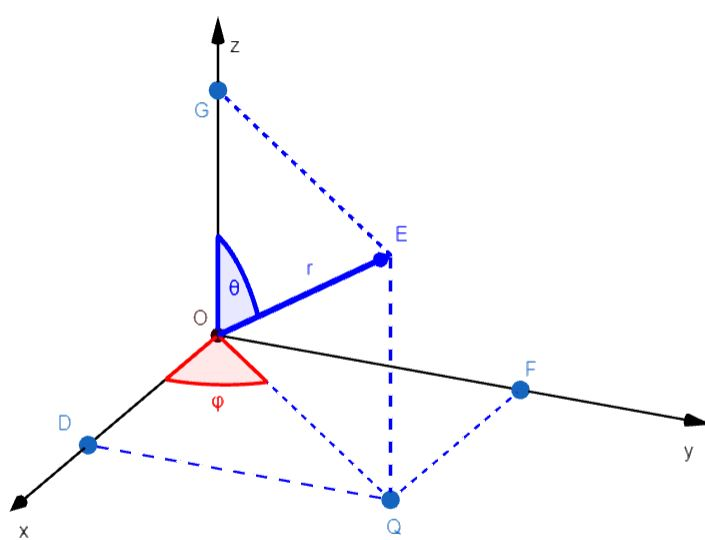
\includegraphics[scale=.6]{spherical.jpg}


\end{minipage}\hfill
\begin{minipage}[t]{0.3\textwidth}
%\centering
\vspace{50pt}
$\left\{ \begin{array}{c}
    x= r\sin \theta \cos \phi \\
     y= r\sin \theta\sin \phi \\
      z= r\cos\theta 
  \end{array} \right.$
\end{minipage}
\caption{Spherical coordinate system}
\label{fig:fig_p23_117_a}
\end{figure}
Partial differentiating of (x,y,z) with respect to (r,$\theta$,$\phi$) gives the Jacobian
\begin{align}
\ J&=
\left| {\begin{array}{ccc}
    \sin \theta \cos \phi & r\cos \theta\cos \phi  & -r\sin \theta \sin \phi\\
    \sin \theta \sin \phi & r\cos \theta\sin \phi  & r\sin\theta \cos\phi\\
    \cos\theta  & -r\sin \theta &0\\
  \end{array} } \right|
  \\
\ &= r^2\sin \theta (\sin^2 \theta\cos^2 \phi + \sin^2 \theta \sin^2 \phi + \cos^2\theta \cos^2\phi + \cos^2\theta\sin^2\phi)\\
\  &= r^2\sin \theta 
\end{align}
J=0: for $r=0$ or $\theta = 0_{\ r \epsilon (-\infty, +\infty)}$ and $J\rightarrow \pm\infty$ or $\mp\infty$ for $r\rightarrow \pm\infty|_{\theta\neq 0}$. But what about the case $r\rightarrow \pm\infty|_{\theta\rightarrow 0}$? This case is not determined as long as no path is chosen in the $(r,\theta)$ configuration space.
$$\blacklozenge$$
\pagebreak[4]

\section{p23-exercise 3.}
\begin{tcolorbox}
If $X, Y,Z$ are the components of a contravariant vector for rectangular Cartesian coordinates in Euclidean 3-space, find it's components for spherical polar coordinates.
\end{tcolorbox}

Be $x^{\alpha}$ the components of a contravariant vector in spherical polar coordinates and $x^{i}$ it's components in rectangular Cartesian coordinates. As we have  
\begin{align}
 \begin{array}{c}
    \ x^{\rho} = \sqrt{x^{j}x^{j}}\\
    \ x^{\theta} = \atan{\frac{x^{2}}{x^{1}}}\\
    \ x^{\phi} = \asin{\frac{x^{3}}{\sqrt{{x^{j}x^{j}}}}}\\
  \end{array} \quad \text{ and } \quad A^{\alpha} = A^{i}\pdv{x^{\alpha}}{x^{i}}
  \end{align}
\begin{align}
\Rightarrow \left[A^{\alpha} \right]=  \left[A^{i}\pdv{x^{\alpha}}{x^{i}}\right] = \left[ {\begin{array}{ccc}
    \ \frac{x^1} { \sqrt{x^{j}x^{j}}} & \frac{x^2} { \sqrt{x^{j}x^{j}}} & \frac{x^3} { \sqrt{x^{j}x^{j}}}\\\\
    -\frac{x^2} { (x^1)^2+(x^2)^2} & \frac{x^1} { (x^1)^2+(x^2)^2}  & 0 \\\\
    -\frac{x^3x^1} { (x^{j}x^{j})\sqrt{(x^1)^2+(x^2)^2}} & -\frac{x^3x^2} { (x^{j}x^{j})\sqrt{(x^1)^2+(x^2)^2}}  & \frac{\sqrt{(x^1)^2+(x^2)^2}} { (x^{j}x^{j})} \\
  \end{array} } \right]\left[ {\begin{array}{c}
    \ A^{1}\\\\
    \ A^{2}\\\\
    \ A^{3}\\\\
  \end{array} } \right]
\end{align}
$$\blacklozenge$$
\pagebreak[4]

\section{p23-exercise 4.}
\begin{tcolorbox}
In a space of three dimensions, how many different expressions are represented by the product $A^{m}_{np} B^{pq}_{rs}C^{s}_{tu}$? How many terms occur in each such expression, when written out explicitly?
\end{tcolorbox}

As we have $V_{3}$ and considering that in $A^{m}_{np} B^{pq}_{rs}C^{s}_{tu}$ the six indices m, n, q, r, t, u are not dummy indices, we get $3^{6}$ different expressions (first choose m: you have three choices, then n: also three choices giving 3x3 possibilities, etc for q, r, t, u).\\
For the second question, as in $A^{m}_{np} B^{pq}_{rs}$ there is only summation on over index (p) we get three terms for this part. As the summation with $A^{m}_{np} B^{pq}_{rs}$ and $C^{s}_{tu}$ occurs only on one index also (s) we get 3x3 terms in the expression.

$$\blacklozenge$$
\pagebreak[4]

\section{p23-exercise 5.}
\begin{tcolorbox}
If A  is an invariant in $V_{n}$, are the second derivatives $\pdv{A}{x^{r}}{x^{s}}$ the components of a tensor?
\end{tcolorbox}

As A is invariant (note: different alphabets in the indices indicates different coordinate systems):
\begin{align}
\ A(x^{\rho}) = A(x^{i})\\
\Rightarrow \pdv{A(x^{\rho})}{x^{i}} = \pdv{A(x^{j})}{x^{i}}
\end{align}
To simplify the notation, we put $A(x^{\rho}) = A^{'}$ and $A(x^{j}) = A^{'}$ then (2) can be written as
\begin{align}
\pdv{A^{'}}{x^{\rho}}\pdv{x^{\rho}}{x^{i}} = \pdv{A}{x^{i}}
 \end{align}
 Conclusion: $\pdv{A}{x^{i}}$ is a covariant tensor. \\\\Consider now $\pdv{A}{x^{i}} = \pdv{A^{'}}{x^{\rho}}\pdv{x^{\rho}}{x^{i}}$. Then,
\begin{align}
\pdv{A}{x^{i}}{x^{j}} &= \pdv{A^{'}}{x^{\rho}}{x^{j}}\pdv{x^{\rho}}{x^{i}}+ \pdv{A^{'}}{x^{\rho}}\pdv{x^{\rho}}{x^{i}}{x^{j}}\\
\Leftrightarrow \pdv{A}{x^{i}}{x^{j}} &= \pdv{A^{'}}{x^{\rho}}{x^{\gamma}}\pdv{x^{\gamma}}{x^{j}}\pdv{x^{\rho}}{x^{i}}+ \pdv{A^{'}}{x^{\rho}}\pdv{x^{\rho}}{x^{i}}{x^{j}}
\end{align}
The first term on the right side, behaves as covariant tensor but the presence of the second term makes that generally, $\pdv{A}{x^{i}}{x^{j}}$ has not a tensor character. This is only when $\pdv{A^{'}}{x^{\rho}}\pdv{x^{\rho}}{x^{i}}{x^{j}}=0$, which means that $x^{\rho}, x^{i}$ are a linear map of each other.
$$\blacklozenge$$
\pagebreak[4]

\section{p23-exercise 6.}
\begin{tcolorbox}
Suppose that in $V_2$ the components of a contravariant tensor field $T^{mn}$ in a coordinate system $x^r$ are 
$$T^{11}=1 \quad T^{12}=0$$
$$T^{21}=1 \quad T^{22}=0$$
Find the components $T^{'mn}$ in a coordinate system $x^{'r}$, where
$$x^{'1} =(x^{1})^2\quad x^{'2} = (x^{2})^2$$
Write down the values of these components in particular at the point $x^1 = 1, x^2 0 =$.
\end{tcolorbox}
As we have a contravariant tensor field :
\begin{align}
\ T^{'mn} =  T^{ij}\pdv{x^{'m}}{x^{i}}\pdv{x^{'n}}{x^{j}}\\
 \begin{array}{ccc}
   \quad \quad \quad \quad  x^{'1} =(x^{1})^2  \Rightarrow & \pdv{x^{'1}}{x^{1}} = 2x^{1} & \pdv{x^{'1}}{x^{2}} = 0\\
\quad \quad \quad \quad x^{'2} =(x^{2})^2  \Rightarrow & \pdv{x^{'2}}{x^{1}} = 0 & \pdv{x^{'2}}{x^{2}} = 2x^{2}\\
  \end{array}\\
  \end{align}
  \begin{align}
  &\Rightarrow T^{'11} = 4(x^{1})^2 + 4(x^{2})^2 \\
  &\Rightarrow T^{'12} = T^{'21}=0 \\
  &\Rightarrow T^{'22} = 4(x^{1})^2 + 4(x^{2})^2
  \end{align}\\\\
  The components in  at the point $x^1 = 1, x^2 = 0$ are
  $$T^{'}(1,0) = \left[{\begin{array}{cc} 4 & 0 \\
    0 & 4 \\ 
    \end{array} } \right]$$
    
    $$\blacklozenge$$
\pagebreak[4]

\section{p24-exercise 7.}
\begin{tcolorbox}
Given that if $T_{mnrs}$ is a covariant tensor, and 
$$ T_{mnrs}+T_{mnsr} = 0$$ in a coordinate system $x^{p}$, establish directly that $$ T^{'}_{mnrs}+T^{'}_{mnsr} = 0$$ in any other coordinate system $x{,q}$.
\end{tcolorbox}
Note: in the following, different alphabets in the indices indicates different coordinate systems.
As we $T_{mnrs}$ is a covariant tensor :
\begin{align}
\ T_{\alpha\beta\gamma\delta} &=  T_{mnrs}\pdv{x^{m}}{x^{\alpha}}\pdv{x^{n}}{x^{\beta}}\pdv{x^{r}}{x^{\gamma}}\pdv{x^{s}}{x^{\delta}}\\
\Rightarrow T_{\alpha\beta\gamma\delta}+T_{\alpha\beta\delta\gamma} &= T_{mnrs}\pdv{x^{m}}{x^{\alpha}}\pdv{x^{n}}{x^{\beta}}\pdv{x^{r}}{x^{\gamma}}\pdv{x^{s}}{x^{\delta}}+ T_{mnrs}\pdv{x^{m}}{x^{\alpha}}\pdv{x^{n}}{x^{\beta}}\pdv{x^{r}}{x^{\delta}}\pdv{x^{s}}{x^{\gamma}}
\end{align}
Now, swap the dummy indices r and s in the second term on the right and as $T_{mnrs} = - T_{mnsr}$:
\begin{align}
\ T_{\alpha\beta\gamma\delta}+T_{\alpha\beta\delta\gamma} &= T_{mnrs}\pdv{x^{m}}{x^{\alpha}}\pdv{x^{n}}{x^{\beta}}\pdv{x^{r}}{x^{\gamma}}\pdv{x^{s}}{x^{\delta}}+ T_{mnsr}\pdv{x^{m}}{x^{\alpha}}\pdv{x^{n}}{x^{\beta}}\pdv{x^{s}}{x^{\delta}}\pdv{x^{r}}{x^{\gamma}}\\
&= (T_{mnrs}+ T_{mnsr})\pdv{x^{m}}{x^{\alpha}}\pdv{x^{n}}{x^{\beta}}\pdv{x^{s}}{x^{\delta}}\pdv{x^{r}}{x^{\gamma}}\\&=0
\end{align}
$$\blacklozenge$$
\pagebreak[4]

\section{p24-exercise 8.}
\begin{tcolorbox}
Prove that if $A_{r}$ is a covariant vector, then $\pdv{A_{r}}{x^{s}} - \pdv{A_{s}}{x^{r}}$ is a skew-symmetric covariant tensor of the second order (use the notation of 1.7).
\end{tcolorbox}
Be $B_{rs} = \pdv{A_{r}}{x^{s}} - \pdv{A_{s}}{x^{r}}$.\\
i) $B_{rs}$ is skew-symmetric:
It is obvious that:$$-B_{rs} = -\pdv{A_{r}}{x^{s}} + \pdv{A_{s}}{x^{r}} = \pdv{A_{s}}{x^{r}}-\pdv{A_{r}}{x^{s}}\equiv B_{sr}$$
ii)  $B_{rs}$ is covariant:\\
\textit{Note: in the following, different alphabets in the indices indicates different coordinate systems.}\\
Let 
\begin{align}
\ C_{\alpha\beta} = (\partial_sA_r - \partial_rA_s)X^r_{\alpha}X^s_{\beta}. 
\end{align}
We know that $A_i= A_{\gamma}X^{\gamma}_i$  as $A_i$ is covariant. Hence,
\begin{align}
\partial_jA_i &= \partial_j A_{\gamma} X^{\gamma}_i + A_{\gamma}\partial_jX^{\gamma}_i\\
\ &= \partial_{\alpha} A_{\gamma} X^{\alpha}_j X^{\gamma}_i + A_{\gamma}\partial_jX^{\gamma}_i
\end{align}
Using (3), we compute the first term in (1)
\begin{align}
\partial_sA_rX^r_{\alpha}X^s_{\beta}&=  \partial_{\rho} A_{\gamma} X^{\rho}_s X^{\gamma}_rX^r_{\alpha}X^s_{\beta}+A_{\gamma}\partial_sX^{\gamma}_rX^r_{\alpha}X^s_{\beta}\\
\ &=  \partial_{\rho} A_{\gamma} X^{\rho}_{\beta} X^{\gamma}_{\alpha}+A_{\gamma}\partial_sX^{\gamma}_rX^r_{\alpha}X^s_{\beta}\\
\ &=  \partial_{\rho} A_{\gamma} \delta^{\rho}_{\beta} \delta^{\gamma}_{\alpha}+A_{\gamma}\partial_sX^{\gamma}_rX^r_{\alpha}X^s_{\beta}\\
\ &=  \partial_{\beta} A_{\alpha} +A_{\gamma}\partial_sX^{\gamma}_rX^r_{\alpha}X^s_{\beta}
\end{align}
In the same way, we get for the second term in (1)
\begin{align}
\partial_rA_sX^s_{\alpha}X^r_{\beta} &=  \partial_{\alpha} A_{\beta} + A_{\gamma}\partial_rX^{\gamma}_sX^r_{\alpha}X^s_{\beta}
\end{align}\\
And thus,
\begin{align}
\ C_{\alpha\beta} =(\partial_sA_r - \partial_rA_s)X^r_{\alpha}X^s_{\beta} &=\partial_{\beta} A_{\alpha} +A_{\gamma}\partial_sX^{\gamma}_rX^r_{\alpha}X^s_{\beta} - \partial_{\alpha} A_{\beta} - A_{\gamma}\partial_rX^{\gamma}_sX^r_{\alpha}X^s_{\beta}\\
\ \Rightarrow \partial_{\beta} A_{\alpha}  - \partial_{\alpha} A_{\beta} &=  (\partial_sA_r - \partial_rA_s)X^r_{\alpha}X^s_{\beta}
\end{align}
So, i) and (10) proves that $\pdv{A_{r}}{x^{s}} - \pdv{A_{s}}{x^{r}}$ is skew-symmetric tensor of the second order.
$$\blacklozenge$$
\pagebreak[4]

\section{p24-exercise 9.}
\begin{tcolorbox}
Let $x^r, \overline{x}^r, y^r,\overline{y}^r $ be four systems of coordinates. Examine the tensor character of $\pdv{x^r}{y^s}$ with respect to the following transformations:\\
i) A transformation $x^r = f^r(\overline{x}^1,\dots,\overline{x}^N)$, with $y^r$ unchanged;\\
ii) A transformation $y^r = g^r(\overline{y}^1,\dots,\overline{y}^N)$, with $x^r$ unchanged;
\end{tcolorbox}
\textit{Note: in the following, different alphabets in the indices indicates different coordinate systems.}\\\\
%Be $A(r,s) = \pdv{x^r}{y^s}$.\\
i) Let's compute the expression $A(\alpha, \beta) = \pdv{x^r}{y^s}\pdv{x^{\alpha}}{x^r}\pdv{x^s}{x^{\beta }}$. Obviously, the right side is an expression of a (possible) mixed tensor of the second order ($\pdv{x^r}{y^s}$) under transformation from the (r) coordinate system to the ($\alpha$) coordinate system. Then, 
\begin{align}
\ A(\alpha, \beta) &= \pdv{x^r}{y^s}\pdv{x^{\alpha}}{x^r}\pdv{x^s}{x^{\beta }}\\
&= \pdv{x^{\alpha}}{y^s}\pdv{x^s}{x^{\beta }}\\
&= \pdv{x^{\alpha}}{y^{\rho}}\pdv{y^{\rho }}{y^s}\pdv{x^s}{x^{\beta }}
\end{align}
If we consider the $\overline{y}^r$ coordinate system as the $y^{\rho }$ coordinate system and as $\overline{y}^r = y^r$ then $\pdv{y^{\rho }}{y^s} = \delta^{\rho}_s$ and we get from (3)
\begin{align}
\ A(\alpha, \beta) &= \pdv{x^{\alpha}}{y^{\rho}}\pdv{y^{\rho }}{y^s}\pdv{x^s}{x^{\beta }}\\
\ &= \pdv{x^{\alpha}}{y^{\rho}}\delta^{\rho}_{s}\pdv{x^s}{x^{\beta }}\\
\ &= \pdv{x^{\alpha}}{y^{\rho}}\pdv{x^{\rho}}{x^{\beta }}\\
\ &= \pdv{x^{\alpha}}{y^{\rho}}\delta^{\rho}_{\beta }\\
\ &= \pdv{x^{\alpha}}{y^{\beta}}\\
\text{(1) and (8)   } \Rightarrow \pdv{x^{\alpha}}{y^{\beta}} &= \pdv{x^r}{y^s}\pdv{x^{\alpha}}{x^r}\pdv{x^s}{x^{\beta }}
\end{align}
So $A(r,s) = \pdv{x^r}{y^s}$ is a mixed tensor of type $A_s^r$\\\\
ii) Let's compute the expression $A(\alpha, \beta) = \pdv{x^r}{y^s}\pdv{y^{\alpha}}{y^r}\pdv{y^s}{y^{\beta }}$. Obviously, the right side is an expression of a (possible) mixed tensor of the second order ($\pdv{x^r}{y^s}$) under transformation from the (r) coordinate system to the ($\alpha$) coordinate system. Then, 
\begin{align}
\ A(\alpha, \beta) &= \pdv{x^r}{y^s}\pdv{y^{\alpha}}{y^r}\pdv{y^s}{y^{\beta }}\\
&= \pdv{x^r}{y^{\rho}}\pdv{y^{\rho}}{y^s}\pdv{y^{\alpha}}{y^r}\pdv{y^s}{y^{\beta }}\\
&= \pdv{x^r}{y^{\rho}}\pdv{y^{\rho}}{y^{\beta}}\pdv{y^{\alpha}}{y^r}\\
&= \pdv{x^r}{y^{\rho}}\delta^{\rho}_{\beta}\pdv{y^{\alpha}}{y^r}\\
&= \pdv{x^r}{y^{\beta}}\pdv{y^{\alpha}}{y^r}\\
&= \pdv{x^r}{x^{\sigma}}\pdv{x^{\sigma}}{y^{\beta}}\pdv{y^{\alpha}}{y^r}
\end{align}
If we consider the $\overline{x}^r$ coordinate system as the $x^{\sigma }$ coordinate system and as $\overline{x}^r = x^r$ then $\pdv{x^{\sigma }}{x^r} = \delta^{\sigma}_r$ and we get from (15)
\begin{align}
\ A(\alpha, \beta) &= \pdv{x^r}{x^{\sigma}}\pdv{x^{\sigma}}{y^{\beta}}\pdv{y^{\alpha}}{y^r}\\
\ &= \delta^r_{\sigma}\pdv{x^{\sigma}}{y^{\beta}}\pdv{y^{\alpha}}{y^r}\\
\ &= \pdv{x^{\sigma}}{y^{\beta}}\pdv{y^{\alpha}}{y^{\sigma}}\\
\ &= \pdv{x^{\sigma}}{y^{\beta}}\delta^{\alpha}_{\sigma}\\
\ &= \pdv{x^{\alpha}}{y^{\beta}}\\
\text{(10) and (19)   } \Rightarrow \pdv{x^{\alpha}}{y^{\beta}} &= \pdv{x^r}{y^s}\pdv{y^{\alpha}}{y^r}\pdv{y^s}{y^{\beta }}
\end{align}
So $A(r,s) = \pdv{x^r}{y^s}$ is a mixed tensor of type $A_s^r$
$$\blacklozenge$$
\pagebreak[4]

\section{p24-exercise 10.}
\begin{tcolorbox}
If $x^r, y^r, z^r$ are three systems of coordinates, prove the follwoing rule for the multiplication of Jacobians.
$$\left|\pdv{x^m}{y^n}\right|\left|\pdv{y^r}{z^s}\right| = \left|\pdv{x^t}{z^u}\right|$$
\end{tcolorbox}
 As we have  
\begin{align}
\pdv{x^t}{z^u} &=\pdv{x^t}{y^k} \pdv{y^k}{z^u}\\
 \left[ { \begin{array}{ccc}
   \ \pdv{x^1}{z^1} & \dots & \pdv{x^1}{z^N}\\
   \vdots & \vdots & \vdots\\
    \pdv{x^N}{z^1} & \dots & \pdv{x^N}{z^N}\\
  \end{array}} \right] &= \left[ { \begin{array}{ccc}
   \ \pdv{x^1}{y^k}\pdv{y^k}{z^1} & \dots & \pdv{x^1}{y^k}\pdv{y^k}{z^N}\\
   \vdots & \vdots & \vdots\\
    \pdv{x^N}{y^k}\pdv{y^k}{z^1}& \dots & \pdv{x^N}{y^k}\pdv{y^k}{z^N}\\
  \end{array}} \right]\\
  &= \left[ { \begin{array}{ccc}
   \ \pdv{x^1}{y^1}& \dots & \pdv{x^1}{y^N}\\
   \vdots & \vdots & \vdots\\
    \pdv{x^N}{y^1}& \dots & \pdv{x^N}{y^k}\\
  \end{array}} \right]\left[ { \begin{array}{ccc}
   \ \pdv{y^1}{z^1} & \dots & \pdv{y^1}{z^N}\\
   \vdots & \vdots & \vdots\\
    \pdv{y^N}{z^1}& \dots & \pdv{y^N}{z^N}\\
  \end{array}} \right]\\
  \ & \Rightarrow \left|\pdv{x^m}{y^n}\right|\left|\pdv{y^r}{z^s}\right| = \left|\pdv{x^t}{z^u}\right|
  \end{align}
$$\blacklozenge$$
\pagebreak[4]


\section{p24-exercise 11.}
\begin{tcolorbox}
Prove that with respect to transformations $$ x^{'r} = C_{rs}x^s$$ where the coefficients are constants satisfying $$C_{mr}C_{ms} = \delta^r_s$$ contravariant and covariant vectors have the same formula of transformation $$ A^{'r} = C_{rs}A^{s} \text{, } A_{,r} = C_{rs}A_{s} $$
\end{tcolorbox}
 i) $ A^{'r} = C_{rs}A^{s}$\\
 
 Be $ A^{'r} = A^{s}\pdv{x^{'r}}{x^s}$ and as $x^{'r} = C_{rs}x^{s}$  we have $\pdv{x^{'r}}{x^s} = C_{rs}$. Hence,$$ A^{'r} = C_{rs}A^{s}$$.\\\\
 i) $ A_{,r} = C_{rs}A_{s}$\\
 Be $ A_{,r} = A_{s}\pdv{x^{s}}{x^{'r}}$ and as $x^{'r} = C_{rs}x^{s}$  we have
\begin{align}
\pdv{x^{'r}}{x^{'t}} &= C_{rs}\pdv{x^{s}}{x^{'t}}\\
\Rightarrow \delta^{r}_{t} &= C_{rs}\pdv{x^{s}}{x^{'t}}
  \end{align}
  Now, multiply (2) by $C_{rq}$. We get,
  \begin{align}
 \delta^{r}_{t}C_{rq} &= C_{rq}C_{rs}\pdv{x^{s}}{x^{'t}}\\
 \ C_{tq} &= C_{rq}C_{rs}\pdv{x^{s}}{x^{'t}}\\
 \text{as }C_{mr}C_{ms} = \delta^r_s \Rightarrow \quad \quad  C_{tq} &= \delta^q_s\pdv{x^{s}}{x^{'t}}\\
 \Rightarrow   C_{tq} &= \pdv{x^{q}}{x^{'t}} \text{  or  }  C_{rs} = \pdv{x^{s}}{x^{'r}}\\
 \text{  as  } A_{,r} = A_{s}\pdv{x^{s}}{x^{'r}} \Rightarrow A_{,r} &= C_{rs}\pdv{x^{s}}{x^{'r}}
  \end{align}
$$\blacklozenge$$
\pagebreak[4]


\section{p25-exercise 12.}
\begin{tcolorbox}
Prove that $$\pdv{ln\left|\pdv{x^m}{y^n}\right|}{x^r} =\pdv{y^m}{x^r}{x^n}\pdv{x^n}{y^m}$$.
\end{tcolorbox}
\begin{lemma}
Be $A$ a square matrix $N\times N$; Be $f$ a $C^1$ function $f:\mathbb{R}^{NxN} \rightarrow \mathbb{R}$. Define $A^{'}$ as $(A^{'}_{ij}) = \dv{f}{A_{ij}}$. Then,$$(ln\left|A\right|)^{'} = (A^{-1})^T \text{ wih }  f =\left|A\right|$$
Proof:\\
By definition of the determinant, we have
\begin{align}
\left|A\right| = A_{iK}C_{K}^i \quad \text{ (no summation on K!)}
\end{align}
with $(C_{K}^i) =  (-1)^{i+K}M^{i}_K$ being the cofactor  of element $A_{iK}$ and $M^{i}_K$ the minor (N-1)x(N-1) matrix associated with the cofactor $A_{K^i}$. Be $C = (C_{ij})$ the NxN matrix formed with all possible cofactor elements  $C_{j}^i \text{  }(i,j = 1 \dots,N)$.\\
We have 
\begin{align}
\ A^{-1} &= \frac{C^T}{\left|A\right|}\\
\Rightarrow (A^{-1})^T &= \frac{C}{\left|A\right|} \\
\text{differentiating (1) }\Rightarrow \pdv{\left|A\right|}{A_{mn}} &= \pdv{A_{iK}}{A_{mn}}C^i_K +A_{iK} \pdv{C^i_K}{A_{mn}}\\
\text{we have for i = m } & \begin{array}{c}
    \pdv{A_{iK}}{A_{mn}} = 1\quad K=n\\
    \pdv{A_{iK}}{A_{mn}} = 0\quad K \neq n\\
  \end{array}
\end{align}
Also, $\forall K: \pdv{C^i_K}{A_{in}} = 0 $ as by definition of the cofactor matrix, $A_{ij} $ is not contained in $C_{ij} $.\\
Hence, (4) becomes
\begin{align}
\pdv{\left|A\right|}{A_{ij}} &= C^i_j\\
\text{But,}\quad \pdv{ln\left|A\right|}{A_{ij}} &= \frac{\pdv{\left|A\right|}{A_{ij}}}{\left|A\right|}\\
\text{(6) and  (7) gives}\quad \pdv{ln\left|A\right|}{A_{ij}} &= \frac{C^i_j}{\left|A\right|}\\
\text{(3) and  (8) gives}\quad \pdv{ln\left|A\right|}{A_{ij}} &= \frac{(A^{-1}_{ij})^T \left|A\right|}{\left|A\right|} = (A^{-1}_{ij})^T \\
\Rightarrow (ln\left|A\right|)^{'} &= (A^{-1})^T
\end{align}
\end{lemma}$$\diamond$$

Now the main proof:\\
Let, 
\begin{align}
\ A \equiv \left[ a_{mn}\right] &= \left[ \pdv{y^m}{x^n}\right]\\
\Rightarrow \pdv{ln\left|A\right|}{x^r} &= \pdv{ln\left|A\right|}{a_{mn}}\pdv{a_{mn}}{x^r}\\
\text{from (10) we get }\quad \pdv{ln\left|A\right|}{a_{mn}} &= (A^{-1})^T_{mn}\\
\text{But A is a Jacobian, so } (A^{-1})_{mn} &= \pdv{x^m}{y^n}\\
\text{ and thus  }(A^{-1})^T_{mn} &=  \pdv{x^n}{y^m}\\
\text{(13) can be written as }  \pdv{ln\left|A\right|}{x^r} &=  \pdv{x^n}{y^m}\pdv{a_{mn}}{x^r}\\
\Rightarrow \pdv{ln\left|A\right|}{x^r} &=  \pdv{x^n}{y^m}\pdv{y^m}{x^r}{x^n}
\end{align}
$$\blacklozenge$$
\pagebreak[4]

\section{p25-exercise 13.}
\begin{tcolorbox}
Consider the quantities $\dv{x^r}{t}$ for a particle moving in the plane. If $x^r$ are the rectangular Cartesian coordinates, are these quantities the components of a contravariant or covariant vector with respect to rotation of the axes? Are they components of a vector with respect to transformation to any curvilinear coordinates (e.g. polar coordinates)?
\end{tcolorbox}
Note: we suppose that by a rotation of the axes, the problem means a fixed rotation and not a rotation varying in time.\\\\
 i) Be $v^{r} = \dv{x^r}{t}$ and consider $v^{\alpha}$  the same object but in another the coordinate system.
 A rotation of the axes implies the linear form
 \begin{align}
 \ &x^{\alpha} = R^{\alpha }_k x^k \quad \text{ with } R^{\alpha }_k \neq R^{\alpha }_k (x^k)\\
 \Rightarrow\quad  & \pdv{x^{\alpha}}{x^r} = R^{\alpha }_k \delta^k_r \\
 \Rightarrow\quad  & R^{\alpha }_r  = \pdv{x^{\alpha}}{x^r} 
 \end{align}
 Consider $v^{\alpha} = \dv{x^{\alpha}}{t}$
 \begin{align}
 v^{\alpha} &= \dv{x^{\alpha}}{t}\\
 \text{(1)   }\Rightarrow\quad v^{\alpha} &= R^{\alpha }_k \dv{x^k}{t}\\
 \Rightarrow\quad v^{\alpha} &= R^{\alpha }_k v^k\\
 \text{(3)   }\Rightarrow\quad v^{\alpha} &= v^k\pdv{x^{\alpha}}{x^r} 
 \end{align}
 Conclusion: $v^k$ is a contravariant vector.\\\\
 ii) Are they components of a vector with respect to transformation to any curvilinear coordinates (e.g. polar coordinates)?\\
We know that 
\begin{align}
\ dx^{\alpha} = \pdv{x^{\alpha}}{x^r}dx^r\\
\Rightarrow \quad \dv{x^{\alpha}}{t} = \pdv{x^{\alpha}}{x^r}\dv{x^r}{t}\\
\Rightarrow \quad v^{\alpha} = v^r\pdv{x^{\alpha}}{x^r}
\end{align}
So $v^r$ is a contravariant vector in general. Note that this proof is more straightforward than the prove in i).
$$\blacklozenge$$
\pagebreak[4]

\section{p25-exercise 14.}
\begin{tcolorbox}
Consider the question raised in No. 13 for the acceleration $\dv[2]{x^r}{t}$.
\end{tcolorbox}
From exercise 13. we know that 

 \begin{align}
 \dv{x^{\alpha}}{t} &= \pdv{x^{\alpha}}{x^r}\dv{x^r}{t}\\ 
 \Rightarrow\quad \dv[2]{x^{\alpha}}{t} &= \dv[2]{x^r}{t}\pdv{x^{\alpha}}{x^r}+ \dv{\pdv{x^{\alpha}}{x^r}}{t}\dv{x^r}{t}\\ 
 &= \dv[2]{x^r}{t}\pdv{x^{\alpha}}{x^r}+ \pdv{x^{\alpha}}{x^r}{x^m}\dv{x^m}{t}\dv{x^r}{t} 
 \end{align}
 The second term on the right does not vanish in general, hence $\dv[2]{x^r}{t}$ has not a tensor character.
$$\blacklozenge$$
\pagebreak[4]

\section{p25-exercise 15.}
\begin{tcolorbox}
It is well known that the equation of an ellipse may be written $$ ax^2+2hxy+by^2 =1$$
What is the tensor character of $a,h, b$ with respect to transformation to any Cartesian coordinates (rectangular or oblique) in the plane?
\end{tcolorbox}
Consider the transformation from a $(w,z)$ coordinate system to a $(x,y)$ coordinate system. For the considered type of transformation we have
\begin {align}
\begin{array}{c}
\ x = \alpha w + \beta z\\
\ y = \gamma w + \delta z\\
  \end{array}\\
\text{consider}\quad \begin{array}{c}
\ ax^2+2hxy+by^2 =1\\
\ pw^2+2qwz+rz^2 =1
  \end{array}
\end{align}
the two representations of the same ellipse in the respective coordinate systems. Plugging (1) in (2):
\begin {align}
%\text{(2)}\quad \Rightarrow\quad ax^2+2hxy+by^2 = pw^2+2qwz+rz^2\\
\ a\alpha^2 w^2 + a 2 \alpha \beta w z + \alpha \beta^2 z^2 +2h \alpha \gamma w^2 +\beta \delta z^2+2h(\alpha \delta + \gamma \beta) w z + b \gamma^2 w^2 + 2 b \gamma \delta w z +\delta^2 z^2 b = 1\\
\end{align}
Rearranging and equating the terms in $w^2, wz, z^2$ in (2) gives
\begin{align}
\ p &= a \alpha^2 + 2 h \alpha \gamma + b \gamma^2\\
\ q &=  a \alpha \beta + h(\alpha \delta + \gamma \beta) + \gamma d\\
\ r &= a \beta^2 + 2 h \beta \delta +b \delta^2
\end{align}
Consider the following objects
\begin {align}
\ (A_{ij}) = \left[ { \begin{array}{cc}
  \ a &  h\\
  \ h   &b\\
  \end{array}} \right] \\
  \ (A_{ij})^{'} = \left[ { \begin{array}{cc}
  \ a^{'}_{11} &  a^{'}_{12}\\
  \ a^{'}_{21}  & a^{'}_{21}\\
  \end{array}} \right] \\
  \text{ we calculate}\quad A^{'}_{ij} = A_{km}\pdv{x^k}{x^{'i}}\pdv{x^m}{x^{'j}}
\end{align}
with $(x^{'1},x^{'2}) = (w, z)$ and $(x^{1},x^{2}) = (x, y)$. We have,
\begin{align}
\ \pdv{x^1}{x^{'1}} &= \alpha, \pdv{x^1}{x^{'2}} = \beta,\pdv{x^2}{x^{'1}} = \gamma,\pdv{x^2}{x^{'2}} = \delta\\
\text{ (10) and (11)}\quad \Rightarrow\ &\begin{array}{c}
  \ a^{'}_{11} = a \alpha^2 + 2 h \alpha \gamma + b \gamma^2 \\
  \ a^{'}_{22} = a \beta^2 + 2 h \delta \beta + b \delta^2 \\
  \ a^{'}_{12} = a^{'}_{21} =a \alpha \beta + h( \alpha \delta + \gamma \beta) + b \gamma \delta \\
  \end{array}
\end{align}
Combining (5), (6), (7) and (12) we get $$ p = a^{'}_{11}, r = a^{'}_{22}, q =  a^{'}_{12} = a^{'}_{21}$$ and so (9) becomes $$  (A_{ij})^{'} = \left[ { \begin{array}{cc}
  \ p &  q\\
  \ q  & r\\
  \end{array}} \right] \\$$
Considering (10) we see that $\left[ { \begin{array}{cc}
  \ a &  h\\
  \ h   &b\\
  \end{array}} \right] $ transforms to $\left[ { \begin{array}{cc}
  \ p &  q\\
  \ q  & r\\
  \end{array}} \right]$ according the rules of a covariant tensor of order two.
$$\blacklozenge$$
\pagebreak[4]

\section{p25-exercise 16.}
\begin{tcolorbox}
Matter is distributed in a plane and $A,B,H$ are the moments and product of inertia with respect to rectangular aces $0xy$ in a plane. Examine the tensor character of the set of quantities $A,B,H$ under rotation of the axes. What notation would you suggest for moments and product of inertia in order to exhibit the tensor character? What simple invariant can be formed from $A,B,H$ ?
\end{tcolorbox}
Consider the transformation from a $(x^1,x^2)$ coordinate system to a $(y^1,y^2)$ coordinate system. For the considered type of transformation we have
\begin {align}
\begin{array}{c}
\ y^1 = \alpha x^1 + \beta x^2\\
\ y^2 = \gamma x^1 + \delta x^2\\
  \end{array}\\
  \text{Be }\quad  \begin{array}{c}
  \ A = \sum_{\rho} m_{\rho} (x^{2,\rho})^2\\
  \ B = \sum_{\rho} m_{\rho} (x^{1,\rho})^2\\
  \ H = \sum_{\rho} m_{\rho} x^{1,\rho} x^{2,\rho}\\
  \end{array}
    \text{and}\quad  \begin{array}{c}
  \ A^{'} = \sum_{\rho} m_{\rho} (y^{2,\rho})^2\\
  \ B^{'} = \sum_{\rho} m_{\rho} (y^{1,\rho})^2\\
  \ H^{'} = \sum_{\rho} m_{\rho} y^{1,\rho} y^{2,\rho}\\
  \end{array}
\end{align}
the moments and product of inertia, $\rho$ being the index of summation over all the points with mass $m_{\rho}$.\\
For the sake of notational simplicty we consider only one point of mass as the linearity of $A, B, H$ related to $\rho$ ensures the validity of the nexts steps for all points in the plane.\\
From (1) and (2) we have:
\begin {align}
\ \frac{A^{'}}{m_{\rho}}  &= \gamma^2 (x^1)^2+2 \gamma \delta x^1 x^2 + \delta ^2 (x^2)^2\\
\  \frac{B^{'}}{m_{\rho}}  &= \alpha^2 (x^1)^2+2 \alpha \beta x^1 x^2 + \beta ^2 (x^2)^2\\
\  \frac{H^{'}}{m_{\rho}}  &= \alpha \gamma (x^1)^2 + (\gamma \beta + \alpha \delta) x^1 x^2 + \beta \delta (x^2)^2\\
\text{Note that} \quad &\begin{array}{cc}
  \pdv{y^1}{x^1} = \alpha & \pdv{y^1}{x^2} = \beta\\ 
	\pdv{y^2}{x^1} = \gamma & \pdv{y^2}{x^2} = \delta\\ 
  \end{array}\\
  \text{(6) in  (4):}\quad &\frac{B^{'}}{m_{\rho}} =  (x^1)^2\pdv{y^1}{x^1} \pdv{y^1}{x^1}  + 2 (x^1)(x^2)\pdv{y^1}{x^1}\pdv{y^1}{x^2} + (x^2)^2\pdv{y^1}{x^2}\pdv{y^1}{x^2}\\
  &=  (x^1)^2\pdv{y^1}{x^1} \pdv{y^1}{x^1}  +  (x^1)(x^2)\pdv{y^1}{x^1}\pdv{y^1}{x^2} + (x^2)(x^1)\pdv{y^1}{x^1}\pdv{y^1}{x^2} + (x^2)^2\pdv{y^1}{x^2}\pdv{y^1}{x^2}
\end{align}
Repeating the same calculations for $\frac{A^{'}}{m_{\rho}}$ and $\frac{H^{'}}{m_{\rho}} $ gives:
\begin {align}
\begin{array}{c}
\frac{A^{'}}{m_{\rho}} =  (x^1)^2\pdv{y^2}{x^1} \pdv{y^2}{x^1}  +  (x^1)(x^2)\pdv{y^2}{x^1}\pdv{y^2}{x^2} + (x^2)(x^1)\pdv{y^2}{x^2}\pdv{y^2}{x^1} + (x^2)^2\pdv{y^2}{x^2}\pdv{y^2}{x^2}\\
\frac{B^{'}}{m_{\rho}} =  (x^1)^2\pdv{y^1}{x^1} \pdv{y^1}{x^1}  +  (x^1)(x^2)\pdv{y^1}{x^1}\pdv{y^1}{x^2} + (x^2)(x^1)\pdv{y^1}{x^1}\pdv{y^1}{x^2} + (x^2)^2\pdv{y^1}{x^2}\pdv{y^1}{x^2}\\
\frac{H^{'}}{m_{\rho}} =  (x^1)^2\pdv{y^1}{x^1} \pdv{y^2}{x^1}  +  (x^1)(x^2)\pdv{y^1}{x^2}\pdv{y^2}{x^1} + (x^2)(x^1)\pdv{y^1}{x^1}\pdv{y^2}{x^2} + (x^2)^2\pdv{y^1}{x^2}\pdv{y^2}{x^2}
  \end{array}
\end{align}
Now, define 
\begin{align}
(K_{ij}) = \left[ { \begin{array}{cc}
  \ (x^1)^2 &  (x^1)(x^2)\\\\
  \ (x^2)(x^1)  & (x^2)^2\\
  \end{array}} \right] \quad \quad (K_{ij})^{'} = \left[ { \begin{array}{cc}
  \ (y^1)^2 &  (y^1)(y^2)\\\\
  \ (y^2)(y^1)  & (y^2)^2\\
  \end{array}} \right]
\end{align}
 Then (9) can be written as
 \begin {align}
\begin{array}{c}
\frac{A^{'}}{m_{\rho}} = (y^1)^2 =  K^{11}\pdv{y^2}{x^1} \pdv{y^2}{x^1}  +  K^{12}\pdv{y^2}{x^1}\pdv{y^2}{x^2} + K^{21}\pdv{y^2}{x^2}\pdv{y^2}{x^1} + K^{22}\pdv{y^2}{x^2}\pdv{y^2}{x^2}\\\\
\frac{B^{'}}{m_{\rho}} = (y^2)^2 =  K^{11}\pdv{y^1}{x^1} \pdv{y^1}{x^1}  +  K^{12}\pdv{y^1}{x^1}\pdv{y^1}{x^2} + K^{21}\pdv{y^1}{x^1}\pdv{y^1}{x^2} + K^{22}\pdv{y^1}{x^2}\pdv{y^1}{x^2}\\\\
\frac{H^{'}}{m_{\rho}} = (y^1)(y^2)  = K^{11}\pdv{y^1}{x^1} \pdv{y^2}{x^1}  +  K^{12}\pdv{y^1}{x^2}\pdv{y^2}{x^1} + K^{21}\pdv{y^1}{x^1}\pdv{y^2}{x^2} + K^{22}\pdv{y^1}{x^2}\pdv{y^2}{x^2}
  \end{array}
  \end{align}
  Hence,
  \begin{align}
\begin{array}{c}
  \ K^{'11}  =  K^{11}\pdv{y^1}{x^1} \pdv{y^1}{x^1}  +  K^{12}\pdv{y^1}{x^1}\pdv{y^1}{x^2} + K^{21}\pdv{y^1}{x^1}\pdv{y^1}{x^2} + K^{22}\pdv{y^1}{x^2}\pdv{y^1}{x^2}\\\\
\ K^{'22} =  K^{11}\pdv{y^2}{x^1} \pdv{y^2}{x^1}  +  K^{12}\pdv{y^2}{x^1}\pdv{y^2}{x^2} + K^{21}\pdv{y^2}{x^2}\pdv{y^2}{x^1} + K^{22}\pdv{y^2}{x^2}\pdv{y^2}{x^2}\\\\
 \ K^{'12} = K^{'21} = K^{11}\pdv{y^1}{x^1} \pdv{y^2}{x^1}  +  K^{12}\pdv{y^1}{x^2}\pdv{y^2}{x^1} + K^{21}\pdv{y^1}{x^1}\pdv{y^2}{x^2} + K^{22}\pdv{y^1}{x^2}\pdv{y^2}{x^2}
  \end{array}
\end{align}
So the object $(K_{ij})\equiv K^{ij}$ transforms according (12) like a contravariant second order tensor.\\

Now, consider $|K^{ij}|$, obviously $|K^{ij}| = (x^1)^2(x^2)^2-(x^1)(x^2)(x^2)(x^1) =0$, but so is also $|K^{'ij}|$.
$$\Rightarrow\quad |K^{ij}| \text{ is an invariant under the considered transformation}$$. 
$$\blacklozenge$$
\pagebreak[4]

\section{p25-exercise 17.}
\begin{tcolorbox}
$S_{nmr}$ is a skew-symmetric tensor in the first two indices.
 $-f_{mnr} + f_{nmr} = S_{mnr}$.
\end{tcolorbox}
From exercise 13. we know that 
\begin{align}
-f_{mnr} + f_{nmr} = S_{mnr}
\end{align}
Swap the indices three times
\begin{align}
\text{i)}\quad n \leftrightarrow r: (1) &\Rightarrow -f_{mrn} + f_{rmn } = S_{mrn}\\
\ &\Leftrightarrow \underbrace{f_{mnr}}_\text{*} + \underbrace{f_{rmn }}_\text{**} = -S_{rmn}\\
\text{ii)}\quad m \leftrightarrow r: (1) &\Rightarrow -f_{rnm} + f_{nrm } = S_{rnm}\\
\ &\Leftrightarrow \underbrace{f_{rmn}}_\text{**} + \underbrace{f_{nrm }}_\text{***} = -S_{nrm}\\
\text{iii)}\quad m \leftrightarrow n: (1) &\Rightarrow -f_{nmr} + f_{mnr } = S_{nmr}\\
\ &\Leftrightarrow \underbrace{f_{nrm}}_\text{***} + \underbrace{f_{mnr }}_\text{*} = -S_{mnr}\\
\text{(3) - (5) + (7):} \quad 2\underbrace{f_{mnr}}_\text{*} &= -S_{rmn}+S_{nrm}-S_{mnr}\\
\ \Leftrightarrow f_{mnr} &= \frac{-S_{rmn}+S_{nrm}-S_{mnr}}{2}
\end{align}
$$\blacklozenge$$
\pagebreak[4]
\chapter{Basic Operations in Riemannian Space}
\pagebreak[4]

\section{p27-exercise}

\begin{tcolorbox}
Take polar coordinates $r, \theta$ in a plane. Draw the infinitesimal triangle with vertices $(r,\theta)$, $(r+dr,\theta)$, $(r,\theta + d\theta)$. Evaluate the square on the hypotenuse of this infinitisimal triangle, and so obtain the metric tensor for the plan for the coordinates$(r, \theta)$.\end{tcolorbox}
\begin{figure}[htp] 
    \centering
\includegraphics[scale=.5]{polar.jpg}
\end{figure}
\begin{align} 
\ ds^2 &= |AB|^2\\
\ &= dr^2 +|CA|^2\\
\ |CA| &= r\sin(d\theta)\approx rd\theta\\
\Rightarrow ds^2 &= dr^2 + r^2d\theta^2\\
\Rightarrow (a_{mn}) &= \begin{pmatrix}
 1& 0 \\
0 & r^2 \\
\end{pmatrix}
\end{align}
$$\blacklozenge$$
\pagebreak[4]

\section{p27-exercise}

\begin{tcolorbox}
Show that if $x^1 = r, x^2 = \theta, x^3 = \phi$, in the usual notation of spherical polar coordinates, then $$ a_{11} =1, a_{22} = r^2, a_{33} = r^2\sin^2\theta$$ and the other components vanish.
\end{tcolorbox}
One can choose to start from $ds^2 = dx^2+dy^2+dz^2$ and then expanding the $dx^i$ along $(r,\theta,\phi)$ but this a rather tedious way. So we use a more geometrical way of deriving the metric\\
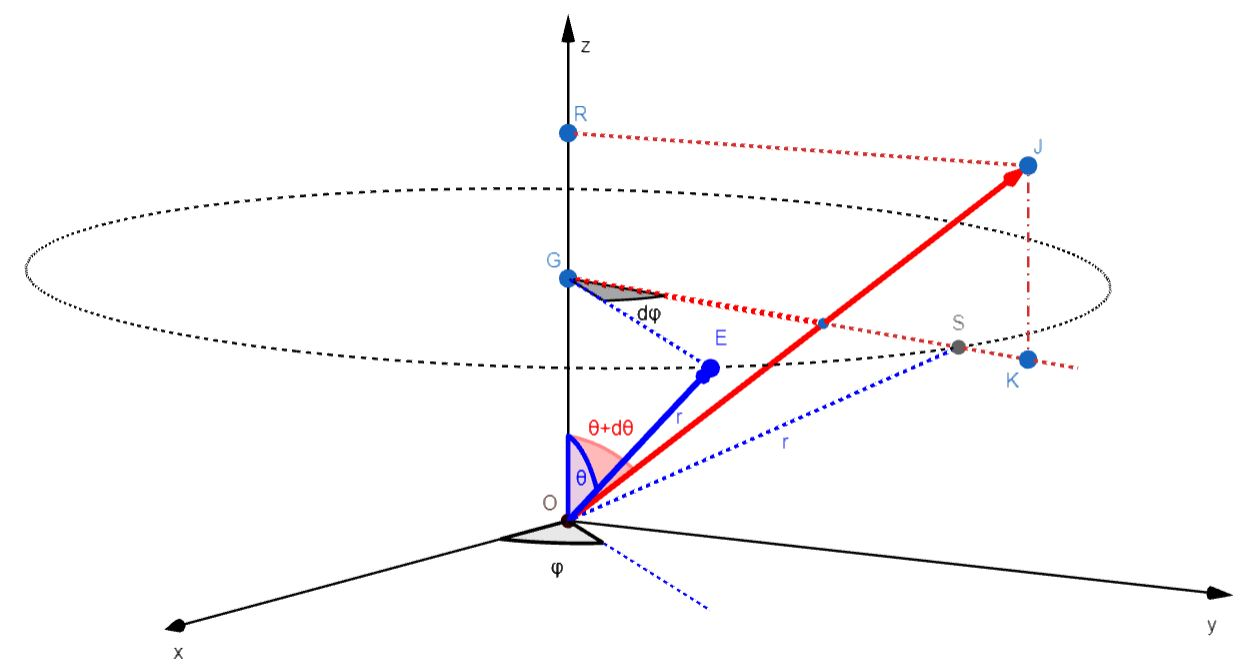
\includegraphics[scale=.6]{sphericalmetric.jpg}\\\\
Consider an infinitesimal displacement of point E to J with $(dr,d\theta, d\phi )$.
\begin{align}
\ ds^2 &= |EJ|^2
\end{align}
As we use infinitesimal displacements we can assume that $$|ES|\perp|GK|\perp|JK|\perp|ES|$$. Hence,
\begin{align}
\ ds^2 = |ES|^2+|SK|^2+|KJ|^2
\end{align}
We have the following relationships
\begin{align}
\left.
\begin{array}{c}
\ |GE| = |GS| = r\sin\theta\\\\
\ |ES| = |GE|d\phi = r\sin\theta d\phi\\\\
\ |GK| = |RJ| = (r+dr)\sin(\theta+d\theta) \\
\ =(r+dr)(\cos(\theta)\sin(d\theta)+\sin(\theta)\cos(d\theta) )\\
\ = (r+dr)(\cos(\theta)d\theta+\sin(\theta))\\
\ = r\cos(\theta)d\theta+r\sin(\theta)+\sin(\theta)dr\\\\
\ |OR| =  (r+dr)\cos(\theta+d\theta)\\
\ = (r+dr)(\cos(\theta)\cos(d\theta)-\sin(\theta)\sin(d\theta))\\
\ = (r+dr)(\cos(\theta)-\sin(\theta)d\theta)\\
\ = r\cos(\theta)-r\sin(\theta)d\theta + \cos(\theta)dr\\\\
\ |OG| = r\cos(\theta)\\\\
\ |JK| = |OR|-|OG| = \cos(\theta)dr-r\sin(\theta)d\theta\\\\
\ |SK| = |GK|-|GS| = r\cos(\theta)d\theta+\sin(\theta)dr\\\\
\end{array}
\right\}
\end{align}
\begin{align}
\left.
\begin{array}{c}
\ |ES|^2 = r^2\sin^2(\theta)d\phi^2\\
\ |SK|^2 = r^2\cos^2(\theta)d\theta^2+\sin^2(\theta)dr^2 +2r\cos(\theta)\sin(\theta)drd\theta \\
\ |JK|^2 = \cos^2(\theta)dr^2+r^2\sin^2(\theta)d\theta^2 -2r\cos(\theta)\sin(\theta)drd\theta\\
\end{array}
\right\}
\end{align}
Hence,
\begin{align}
\ ds^2 &= |ES|^2+|SK|^2+|KJ|^2\\
&= \left\{ \begin{array}{c} r^2\sin^2(\theta)d\phi^2 \\ +r^2\cos^2(\theta)d\theta^2+\sin^2(\theta)dr^2 +2r\cos(\theta)\sin(\theta)drd\theta\\+r^2\sin^2(\theta)d\theta^2+\cos^2(\theta)dr^2 -2r\cos(\theta)\sin(\theta)drd\theta\\
\end{array}
\right.\\
\ &\Rightarrow ds^2= dr^2 + r^2d\theta^2 + r^2\sin^2(\theta)d\phi^2\\
\ & \Rightarrow (a_{mn}) = \begin{pmatrix}
 1& 0 & 0\\
0 & r^2 & 0 \\
0 & 0 & r^2\sin^2\theta \\
\end{pmatrix}
\end{align}
$$\blacklozenge$$
\newpage


\section{p27-exercise}

\begin{tcolorbox}
Starting from 3.103, show that $$a_{mn} = \pdv{y^1}{x^m}\pdv{y^1}{x^n}+\pdv{y^2}{x^m}\pdv{y^2}{x^n}+\pdv{y^3}{x^m}\pdv{y^3}{x^n}$$ and calculate the quantities for a sphere, taking as curvilinear coordinates on he sphere $$x^1 = y^1 , x^2 = y^2$$
\end{tcolorbox}
We have
\begin{align}
\text{(2.103)}\quad &\Rightarrow y^1 = x^1 , y^2 = x^2, y^3 = f^3(x^1,x^2)\\
\text{surface = sphere}\quad &\Rightarrow y^3 = \pm \sqrt{R^2 -(x^1)^2-(x^2)^2}\\
\ ds^2 &= (dx^1)^2+(dx^2)^2+(dx^3)^2\\
\ \text{(1) and (2)}\quad& \Rightarrow \left\{ \begin{array}{c} 
\ dy^1 = dx^1\\\\
\ dy^2 = dx^2\\\\
\ dy^3 = \pm \frac{1}{2} \frac{-2x^1dx^1 - 2x^2dx^2}{\sqrt{R^2 -(x^1)^2-(x^2)^2}}\\\\
\end{array}
\right.\\
\Rightarrow ds^2 & = (dx^1)^2 +  (dx^2)^2 + \frac{(x^1)^2(dx^1)^2 + (x^2)^2(dx^2)^2  + 2 x^1x^2dx^1dx^2}{R^2 -(x^1)^2-(x^2)^2}
\end{align}
\begin{align}
\Leftrightarrow ds^2 & = \frac{(R^2 - (x^2)^2) (dx^1)^2 + (R^2 -(x^1)^2) (dx^2)^2  + 2 x^1x^2dx^1dx^2}{R^2 -(x^1)^2-(x^2)^2}
\end{align}\\
\begin{align}
\Rightarrow (a_{mn}) &= \frac{1}{R^2 -(x^1)^2-(x^2)^2}\begin{pmatrix}
 R^2 - (x^2)^2&x^1x^2 \\
x^1x^2 & R^2 - (x^1)^2 \\
\end{pmatrix}
\end{align}
$$\blacklozenge$$
\newpage


\section{p30-clarification 2.202}

\begin{tcolorbox}
           $$\quad\quad a_{mr}\Delta^{ms} = a_{rm}\Delta^{sm} = \delta^s_r a$$
\end{tcolorbox}
Case 1: $r =s$\\
We have, $a_{Rm}\Delta^{Rm}$ (no summation on R) is the definition of the determinant of A developed along the row R: OK.\\\\
Case 2: $r \neq s$\\
Consider
\begin{align}
\ A &= \begin{pmatrix}
 a_{11} & a_{12}&\dots&a_{1N} \\
a_{21} & a_{22}&\dots&a_{2N} \\
\vdots & \vdots &\vdots & \vdots \\
a_{N1} & a_{N2}&\dots&a_{NN} \\
\end{pmatrix}
\end{align}
and consider the matrix $A^,$
\begin{align}
\ A^, &= \begin{pmatrix}
 a_{11} & a_{12}&\dots&a_{1N} \\
 \vdots & \vdots &\vdots & \vdots \\
a_{R1} & a_{R2}&\dots&a_{RN} \\
\vdots & \vdots &\vdots & \vdots \\
a_{R1} & a_{R2}&\dots&a_{RN} \\
\vdots & \vdots &\vdots & \vdots \\
a_{N1} & a_{N2}&\dots&a_{NN} \\
\end{pmatrix}
\begin{array}{c}
\ \vdots\\
\ \vdots\\
\leftarrow S^{th}\text{ row}\\
\vdots\\
\leftarrow R^{th}\text{ row}\\
\ \vdots\\
\ \vdots\\
\end{array}
\end{align}
This matrix corresponds to the way $a_{Rm}\Delta^{Sm}$ is computed. Indeed with the factor $a_{Rm}$ is not associated it's own cofactor $\Delta^{Rm}$ but the cofactor of the $m^{th}$ column in row $S$. Replacing the $S^{th}$ row with the row $R$ and calculating it's determinant is the same as calculating $a_{Rm}\Delta^{Sm}$\\
But, $|A^,| = 0$ as we have two identical rows. So, $a_{Rm}\Delta^{Sm} = 0$\\\\
Conclusion : The same reasoning can be applied when expanding the determinant along the columns instead of the rows we have indeed $\quad\quad a_{mr}\Delta^{ms} = a_{rm}\Delta^{sm} = \delta^s_r a$.
$$\blacklozenge$$
\newpage


\section{p31-exercise}

\begin{tcolorbox}
Show that if $a{mn} = 0$ for $m\neq n$, then $$a^{11} = \frac{1}{a_{11}}, a^{22} = \frac{1}{a_{22}}, \dots, a¨{12} = 0, \dots$$
\end{tcolorbox}
We have to prove that:
\begin{align}
\ a^{ij} = \left\{\begin{array}{cc}
\frac{1}{a_{ij}} & \text{: }i=j\\
\ 0 & \text{: }i \neq j
\end{array}\right.
\end{align}
From 2.204:
\begin{align}
a_{mR}a_{mS} = \delta^S_R
\end{align}
i) Be $R \neq S$
\begin{align}
\text{(2) }\quad \Rightarrow a_{mR}a_{mS} &= 0\\
\text{but } \quad a_{mR} &=0\quad \forall m \neq R\\
\Rightarrow a_{RR}a^{RS} = 0
\end{align}
but $a_{RR} \neq 0$ ($a_{RR}$ can't be $0$ as the metric tensor would degenerate  if $a_{mn} = 0\quad \forall m \neq n$
\begin{align}
\Rightarrow a^{Rs} = 0\\\\
\end{align}

i) Be $R = S$
\begin{align}
\text{(2) }\quad \Rightarrow a_{mR}a_{mR} &= 1\\
\text{but } \quad a_{mR} &=0\quad \forall m \neq R\\
\Rightarrow a_{RR}a^{RR} = 1\\
\Rightarrow a^{RR} = \frac{1}{a_{RR}}
\end{align}
$$\blacklozenge$$
\newpage

\section{p31-exercise}

\begin{tcolorbox}
Find the components of $a^{mn}$ for spherical polar coordinates in Eulidean 3-space.
\end{tcolorbox}
We have (see exercise page 27):
\begin{align}
\ (a_{mn}) = \begin{pmatrix}
 1& 0 & 0\\
0 & r^2 & 0 \\
0 & 0 & r^2\sin^2\theta \\
\end{pmatrix}
\end{align}
As $a_{mn} = 0 \quad \forall m \neq n$ we deduce (see previous exercise p31)
\begin{align}
\ (a^{mn}) = \begin{pmatrix}
 1& 0 & 0\\
0 & \frac{1}{r^2} & 0 \\
0 & 0 & \frac{1}{r^2\sin^2\theta)}\\
\end{pmatrix}
\end{align}
$$\blacklozenge$$
\newpage

\section{p32-exercise}

\begin{tcolorbox}
Find the mixed metric tensor  $a^{.n}_m$ obtained from $a_{mn}$ by raising the second subscript
\end{tcolorbox}
We have :
\begin{align}
\ a_{i}^{.j} &=  a_{in}a^{nj}\\
\ &=  a_{in}a^{jn}\quad a^{jn} \text{  is symmetric}\\
\ &= \delta^j_i \quad \text{ (see 2.205 pg. 30)}\\
\ &\Rightarrow a_{i}^{.j} = \delta^j_i 
\end{align}
$$\blacklozenge$$
\newpage

\section{p32-clarification 2.214}
\begin{tcolorbox}
          $$ \pdv{a}{a_{mn}} = a a^{mn}$$
\end{tcolorbox}
Put $a_{MN}\equiv a_{mn}$. By definition, we have
\begin{align}
\  a\equiv |a_{mn}|  &= a_{Mk}\Delta^{Mk}\quad\text{(develop determinant along row M)}\\
\ &\Rightarrow \pdv{a}{a_{mn}} = \pdv{a_{Mk}}{a_{mn}}\Delta^{Mk} + a_{Mk}\pdv{\Delta^{Mk}}{a_{mn}}\\
\text{but}\quad &\pdv{a_{Mk}}{a_{mn}} = \left\{\begin{array}{c}
\ 1\quad\text{if} \quad k = N\\
\ 0\quad\text{if} \quad k \neq N\\
\end{array}\right.\\
\text{and}\quad &\pdv{\Delta^{Mk}}{a_{mn}} = 0 \quad \forall k \text{ as } \Delta^{Mk} \text{does not contain the row with } a_{mn} \text{ as element.}\\
\ & \text{(3) and (4)}\quad  \Rightarrow \pdv{a}{a_{mn}} = \Delta^{MN}\\ 
\ &  a^{mn} = \frac{\Delta^{mn}}{a}\quad\text{by definition (see 2.203 page 30)}\\
\ & \Rightarrow \pdv{a}{a_{mn}} = aa^{mn}
\end{align} 
$$\blacklozenge$$
\newpage


\section{p32-exercise}
\begin{tcolorbox}
Prove that $a_{mn}a^{mn} = N$.
\end{tcolorbox}
From 2.204, we have
\begin{align}
\ a_{mr}a^{ms} &= \delta^s_r\\
\text{Consider} \quad a_{mR}a^{mR} &= 1\\
\text{We can repeat (2) for R = 1,2,...,N} \quad \Rightarrow a_{mr}a^{mr} &= N\\
\end{align}
$$\blacklozenge$$
\newpage


\section{p33-exercise}
\begin{tcolorbox}
Show that in Euclidean 3-space with rectangular Cartesian coordinates, the definition 2.301 coincides with the usual definition of the magnitude of a vector.
\end{tcolorbox}
The length of an arbitrary vector in Euclidean 3-space with rectangular Cartesian coordinates, is
\begin{align}
\ ds^2 = (dy^1)^2 + (dy^2)^2 (dy^2)^2
\end {align}
From 2.301, it is obvious that the metrixc tensor can be expressed as,
\begin{align}
\begin{pmatrix}1 & 0 &0 \\ 0 & 1 &0\\0 & 0 &1  \\ \end{pmatrix} 
\end{align}
$$\blacklozenge$$
\newpage


\section{p34-exercise}
\begin{tcolorbox}
A curve in Euclidean 3-space has the equations $$ x^1 =  a \cos(u), x^2 = a\sin(u), x^3 = bu$$ where $x^1, x^2,x^3$ are rectangular Cartesian coordinates,$u$ is a parameter, and $a, b$ are positive constants. Find the length of this curve between the point $u = 0$ and $u = 2\pi$.
\end{tcolorbox}
The metric tensor has the following form,
\begin{align}
\ (a_{ij}) &= \begin{pmatrix}1 & 0 &0 \\ 0 &1 &0\\0 & 0 &1  \\ \end{pmatrix} \\
\text {and  (2.306)  }\quad s &= \int^{2\pi}_0[\epsilon a_{mn}p^mp^n]^{\frac{1}{2}}du
\end{align}
with
\begin{align}
\ p^1 = \dv{x^1}{u} = -a\sin(u), \quad p^2 = \dv{x^2}{u} = a\cos(u), \quad p^3 = \dv{x^3}{u} = b
\end{align}
Hence (2) becomes
\begin{align}
s &= \int^{2\pi}_0\epsilon[a^2 \sin^2(u) + a^2\cos^2(u) + b^2]^{\frac{1}{2}}du\\
\ &= \int^{2\pi}_0\epsilon[a^2+  b^2]^{\frac{1}{2}}du\\
\ &= [a^2+  b^2]^{\frac{1}{2}} \left. u\right|^{2\pi}_0\\
\ &= 2\pi[a^2+  b^2]^{\frac{1}{2}} 
\end{align}
$$\blacklozenge$$
\newpage

\section{p36-clarification 2.314}
\begin{tcolorbox}
Going from 2.313 to 2.314 yields because both $X^m$ and $Y^m$ are unit vectors and by definition of the magnitude (see 2.301) both  $a_{mn}X^mX^n$ and $a_{mn}Y^mY^n$ are 1 (also due to the fact that only a positive definite metric tensor is considered, $\epsilon = 1$).
\end{tcolorbox}
$$\blacklozenge$$
\newpage

\section{p37-exercise}

\begin{tcolorbox}
Show that the small angle between unit vectors $X^r$ and $X^r + dX^r$ (these increments being infenitesimal) is given by $$ \theta^2 = a_{mn}X^mX^n$$
\end{tcolorbox}
\begin{figure}[htp] 
    \centering
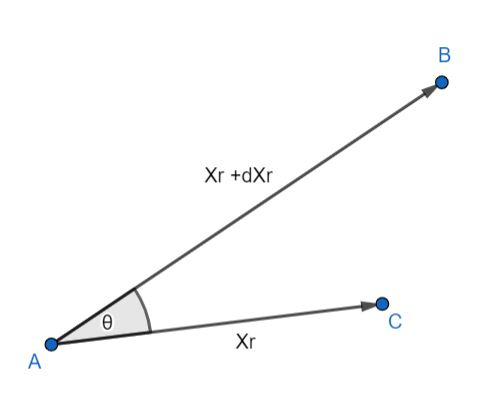
\includegraphics[scale=.5]{Exp37_1.jpg}
\end{figure}
By definition (2.302 page 33)
\begin{align} 
\ |BC|^2 =\epsilon a_{mn}dX^mdX^n\\
\end{align}
We can drop $\epsilon = 1$ as the considered space is positive definite.\\
As $\theta$ is infinitesimal, we can state
\begin{align}
\ |BC| &\approx |AC|\theta\\
\text{ and } \quad |AC| &= X^r = 1\quad  \text{(as } X^r \text{ is a unit vector)}\\
\Rightarrow \theta^2 &= a_{mn}dX^mdX^n
\end{align}
$$\blacklozenge$$
\newpage


\section{p39-clarification 2.409}

\begin{tcolorbox}
We clarify the integration by parts in the derivation of the general  geodesic equation.
\end{tcolorbox}
We have 
\begin{align}
\int d(A.B) &= \int AdB + \int BdA\\
\Rightarrow  \int AdB &= \int BdA -  \int d(A.B)\
\end{align}
Now, substitute 2.407 in 2.406, we get
\begin{align}
\dv{L}{v} &= \int \pdv{(\epsilon w)^{\frac{1}{2}}}{x^r} \pdv{x^r}{v} du +  \int \pdv{(\epsilon w)^{\frac{1}{2}}}{p^r} \pdv{p^r}{v} du\\
\ &= \int \pdv{(\epsilon w)^{\frac{1}{2}}}{x^r} \pdv{x^r}{v} du +  \int \pdv{(\epsilon w)^{\frac{1}{2}}}{p^r} \pdv{\pdv{x^r}{v}}{u} du\\
&= \int \pdv{(\epsilon w)^{\frac{1}{2}}}{x^r} \pdv{x^r}{v} du +  \int \pdv{(\epsilon w)^{\frac{1}{2}}}{p^r} d(\pdv{x^r}{v})
\end{align}
To integrate by parts the second term in (5) we put in (2)
$$A= \pdv{(\epsilon w)^{\frac{1}{2}}}{p^r} \quad \text{and } B = \pdv{x^r}{v}$$
\begin{align}
\int \pdv{(\epsilon w)^{\frac{1}{2}}}{p^r} d(\pdv{x^r}{v}) &= \int AdB \\
\ & = \int BdA -  \int d(A.B)\\
\ &= \pdv{(\epsilon w)^{\frac{1}{2}}}{p^r}\left.\pdv{x^r}{v}\right|_{u_0}^{u_1} - \int \pdv{x^r}{v}d(\pdv{(\epsilon w)^{\frac{1}{2}}}{p^r} )\\
\ &= \pdv{(\epsilon w)^{\frac{1}{2}}}{p^r}\left.\pdv{x^r}{v}\right|_{u_0}^{u_1} - \int \pdv{x^r}{v}\pdv{\pdv{(\epsilon w)^{\frac{1}{2}}}{p^r} )}{u}du
\end{align}
Replacing (9) in (5) gives the formulea 2.409.
$$\blacklozenge$$
\newpage

\section{p41-exercise}
\begin{tcolorbox}
Prove the following identities: $$ [mn,r] = [nm,r], \quad [rm,n]+[rn,m] = \partial_r a_{mn}$$
\end{tcolorbox}
\begin{align}
\ [mn,r] &= \frac{1}{2}(\partial_{n} a_{mr}+ \partial_{m} a_{nr} - \partial_{r} a_{mn})\\
\ &= \frac{1}{2}(\partial_{m} a_{nr} + \partial_{n} a_{mr}  - \partial_{r} a_{nm})\\
\ &=[nm,r] 
\end{align}
and 
\begin{align}
\ [rm,n] + [rn,m]&= \frac{1}{2}(\partial_{r} a_{mn}+ \partial_{m} a_{rn} - \partial_{n} a_{rm} + \partial_{n} a_{rm}+ \partial_{r} a_{mn} - \partial_{m} a_{rn})\\
\ &= \frac{1}{2}(\partial_{r} a_{mn}+\partial_{r} a_{mn})\\
\ &=\partial_{r} a_{mn}
\end{align}
$$\blacklozenge$$
\newpage

\section{p42-exercise}
\begin{tcolorbox}
Prove that  $$ [mn,r] = a_{rs}\Gamma^s_{mn}$$
\end{tcolorbox}
\begin{align}
\ a_{rs}\Gamma^s_{mn} & = a_{rs}a^{sk}[mn,k]\\
\ & = \delta^k_r[mn,k]\\
\ &= [mn,r]
\end{align}
$$\blacklozenge$$
\newpage

\section{p42-clarification on 2.430}
\begin{tcolorbox}
... This may proved without difficulty by starting with 2.427, in which $\lambda$ is a known function of $u$ , and defining $s$ by the relation$$ s = \int^u_{u_0}(exp\int^v_{v_0} \lambda(w)dw)dv$$ $u_0, v_0$ being constants....
\end{tcolorbox}
\begin{align}
\text{see 2.428 :} \quad  \lambda (u)=-\frac{\dv[2]{u}{s}}{(\dv{u}{s})^2}\\
\end{align}
We suppose $u(s)$ continuous by parts with continuous inverse.
\begin{align}
\Rightarrow \dv{s}{u} &= \frac{1}{\dv{u}{s}}\\
\Rightarrow \dv[2]{s}{u}&= \dv{(\frac{1}{\dv{u}{s}})}{s}\dv{s}{u}\\
\ & = -\frac{\dv[2]{u}{s}}{(\dv{u}{s})^2}\dv{s}{u}\\
\Rightarrow \frac{\dv[2]{s}{u}}{\dv{s}{u}} &= - \frac{\dv[2]{u}{s}}{(\dv{u}{s})^2}  
\end{align}
By definition (2.428)
\begin{align}
\ \lambda (u) &= - \frac{\dv[2]{u}{s}}{(\dv{u}{s})^2}\\
\text{hence by (6) and (7):}\quad  \lambda (u) &= \frac{\dv[2]{s}{u}}{\dv{s}{u}}\\
\text{in (8) put}\quad y &= \dv{s}{u} \\
\text{ and so} \quad \lambda (w)  &= \frac{y^,}{y}\\
\Rightarrow \int \frac{y^,}{y}dw &= \int \lambda (w)dw\\
\Leftrightarrow \int d(lny) &= \int \lambda (w)dw\\
\Rightarrow \left. ln(y) \right|^v_{v_0} &= \int^v_{v_0} \lambda (w)dw\\
\Rightarrow y  &= exp(\int^v_{v_0} \lambda (w)dw) + C
\end{align}
Taking into account (9), we get:
\begin{align}
\dv{s}{v}  &= exp(\int^v_{v_0} \lambda (w)dw) + C\\
\Rightarrow \left. s \right|^u_{u_0} &=\int^u_{u_0}  exp(\int^v_{v_0} \lambda (w)dw)dv +Cu + B^,\\
\Leftrightarrow  s  &=\int^u_{u_0}  exp(\int^v_{v_0} \lambda (w)dw)dv +Cu + B
\end{align}
We show tha we have to put $C=0$ and can drop the constant $B$. Remember by (8)
\begin{align}
\lambda (u) &= \frac{\dv[2]{s}{u}}{\dv{s}{u}}\\
\text{by (17)} \quad \dv{s}{u}  &=exp(\int^u_{u_0} \lambda (w)dw) +C\\
\text{and}\quad \dv[2]{s}{u}  &= \lambda (u) exp(\int^u_{u_0} \lambda (w)dw) \\
\text{hence by (18), (19) and (20):} \quad \lambda (u)&= \frac{\lambda (u) exp(\int^u_{u_0} \lambda (w)dw)}{exp(\int^u_{u_0} \lambda (w)dw) +C}
\end{align}
So, whatever the constant B, the relation (18) is correct on the condition that C=0. 
So, indeed, we can choose the independent variable $s$ as
$$s  =\int^u_{u_0}  exp(\int^v_{v_0} \lambda (w)dw)dv $$ 
$$\blacklozenge$$
\newpage

\section{p42-clarification on 2.430}
\begin{tcolorbox}
After 2.430 it is stated:\\
\it{"No matter what values these constants have, 2.424 is satisfied, and by adjusting the constant $v_0$, we can ensure that $a_{mn}\dv{x^m}{s}\dv{x^n}{s} = \pm1$ along $C$, so that $s$ is actually the arc length."}
\end{tcolorbox}
We first prove that 2.4.24 is satisfied, no matter what values the constants take. We have
\begin{align}
\text{(2.430) } \quad  &s =\int_{u_0}^u(exp\int_{v_0}^v \lambda (w)dw)dv\\
\text{and (2.427)} \quad &\dv[2]{x^r}{u} + \Gamma^r_{mn}\dv{x^m}{u}\dv{x^n}{u} =  \lambda \dv{x^r}{u}
\end{align}
In (2) we can write the first term as
\begin{align}
\quad \dv[2]{x^r}{u} &= \dv{(\dv{x^r}{u})}{s}\dv{s}{u} \\
\text{with } \quad \dv{(\dv{x^r}{u})}{s} &=  \dv{(\dv{x^r}{s}\dv{s}{u})}{s} = \dv[2]{x^r}{s}\dv{s}{u}+\dv{x^r}{s}\dv{(\dv{s}{u})}{s} 
\end{align}
Assuming the curve smooth, we have
\begin{align}
\dv{(\dv{s}{u})}{s} & = \dv{(\frac{1}{\dv{u}{s}})}{s} = -\frac{\dv[2]{u}{s}}{(\dv{u}{s})^2}= \lambda
\end{align}
Putting (4) and (5) in (3) we get
\begin{align}
\dv[2]{x^r}{u} &= \dv[2]{x^r}{s} \left ( \dv{s}{u}\right )^2 + \lambda\dv{x^r}{s}\dv{s}{u}
\end{align}
Plugging (6) in 2.427 gives:
\begin{align}
\dv[2]{x^r}{s} \left (\dv{s}{u}\right )^2 + \lambda\dv{x^r}{s}\dv{s}{u} +\Gamma^r_{mn}\dv{x^m}{s}\dv{x^n}{s}\left (\dv{s}{u}\right )^2  &=  \lambda \dv{x^r}{s}\dv{s}{u}\\
\Leftrightarrow \dv[2]{x^r}{s} \left (\dv{s}{u}\right )^2 +\Gamma^r_{mn}\dv{x^m}{s}\dv{x^n}{s}\left (\dv{s}{u}\right )^2  &=  0
\end{align}
We can assume that $\dv{s}{u} $ does not become $0$ or $\pm \infty$ along the curve by choosing an adequate constant $v_0$. Indeed, from (2.430) we get
\begin{align}
\dv{s}{u}  &= exp(\int_{u_0}^u \lambda (w)dw)\\
\ &= \frac{\phi (u)}{\phi (u_0)}
\end{align}
with $\phi (u_0) =  e^{\theta(u_0)}$, $\theta(u)$ being the indefinite integral $\int \lambda (w)dw $.\\
So, it is sufficient to choose $v_0$ so that $\theta(u_0)$ does not become  $\pm \infty$ to ensure that $\dv{s}{u} \ne 0$ or $ \ne \pm \infty$ along the curve and so we have from (8)
\begin{align}
\dv[2]{x^r}{s} +\Gamma^r_{mn}\dv{x^m}{s}\dv{x^n}{s}  &=  0\end{align}
which is the definition (2.424) of a geodesic.\\\\
The same reasoning about $\dv{s}{u} \ne 0$ can be made to prove that $a_{mn}\dv{x^m}{s}\dv{x^n}{s} = \pm1$ along $C$. Indeed, by definition (2.305):
\begin{align}
\ ds = &\left[ \epsilon a_{mn}\dv{x^m}{u}\dv{x^n}{u}\right]^\frac{1}{2}\\
\text{ equating with (9)} \quad   &\left[ \epsilon a_{mn}\dv{x^m}{u}\dv{x^n}{u}\right]^\frac{1}{2} =                 exp(\int_{u_0}^u \lambda (w)dw)\\
\Rightarrow \quad &\epsilon a_{mn}\dv{x^m}{s}\dv{x^n}{s}\left (\dv{s}{u}\right )^2 =  \left[ exp(\int_{u_0}^u \lambda (w)dw) \right]^2\\
\text{but} \quad &\dv{s}{u} = exp(\int_{u_0}^u \lambda (w)dw)\\
\text{ and so, (9) becomes} \quad &\epsilon a_{mn}\dv{x^m}{s}\dv{x^n}{s}\left (\dv{s}{u}\right )^2 =  \left (\dv{s}{u}\right )^2\\
\Rightarrow \quad & a_{mn}\dv{x^m}{s}\dv{x^n}{s}=\epsilon
\end{align}
$$\blacklozenge$$
\newpage


\section{p43-clarification }
\begin{tcolorbox}
$$\lambda = \Gamma^N_{\mu \nu}\dv{x^{\mu}}{x^N} \dv{x^{\nu}}{x^N} + 2\Gamma^N_{\mu N}\dv{x^{\mu}}{x^N}+\Gamma^N_{N N} $$
\end{tcolorbox}
We start with 2.427 with $r=N$
\begin{align}
\ &\dv[2]{x^N}{{x^{N}}} + \Gamma^N_{\mu\nu}\dv{x^{\mu}}{x^N} \dv{x^{\nu}}{x^N} = \lambda \dv{x^N}{x^N}\\
\Rightarrow\quad &\Gamma^N_{\mu\nu}\dv{x^{\mu}}{x^N} \dv{x^{\nu}}{x^N} = \lambda \quad \text{(as}\quad \dv[2]{x^N}{{x^{N}}} = 0 \quad \dv{x^N}{x^N} = 1 \text{)}
\end{align}
But (2) is only valid with the dummy indices $\mu$ and $\nu$ spanning the whole dimension $(1,2,\dots N)$, but by choice $\mu,\nu \quad \epsilon \quad (1,2, \dots, N-1)$. We have thus to add in the left term of (2) the cases
\begin{align}
\left\{ \begin{array}{cc}
\Gamma^N_{N\nu}& \nu = (1,2,\dots ,N-1)\\\\
\Gamma^N_{\mu N}& \mu = (1,2,\dots ,N-1)\\\\
\Gamma^N_{NN}& \\
\end{array} \right.\\
\text{(2) becomes } \quad \Gamma^N_{\mu\nu}\dv{x^{\mu}}{x^N} \dv{x^{\nu}}{x^N} + \Gamma^N_{N \nu}\dv{x^N}{x^N} \dv{x^{\nu}}{x^N} + \Gamma^N_{\mu N}\dv{x^{\mu}}{x^N} \dv{x^{N}}{x^N} + \Gamma^N_{NN}\dv{x^{N}}{x^N} \dv{x^{N}}{x^N}= \lambda\\
\Rightarrow   \quad \Gamma^N_{\mu\nu}\dv{x^{\mu}}{x^N} \dv{x^{\nu}}{x^N} + \Gamma^N_{N \nu}\dv{x^{\nu}}{x^N} + \Gamma^N_{\mu N}\dv{x^{\mu}}{x^N}+ \Gamma^N_{NN} = \lambda
\end{align}
As $\Gamma^N_{\mu N}$ is symmetric on the lower indices and $\mu$, $\nu$ being dummy indices:
\begin{align}
\lambda  =\Gamma^N_{\mu\nu}\dv{x^{\mu}}{x^N} \dv{x^{\nu}}{x^N} + 2\Gamma^N_{N \nu}\dv{x^{\nu}}{x^N} +\Gamma^N_{NN}
\end{align}
The other $N-1$ equation for $r= 1,\dots, N-1$ can be deduced following the same reasoning.
$$\blacklozenge$$
\newpage


\section{p45-clarification }
\begin{tcolorbox}
$ f_r \equiv a_{rm}\dv[2]{x^m}{u} +[mn,r]\dv{x^m}{u}\dv{x^n}{u}$ is covariant and 
$ f^r \equiv \dv[2]{x^m}{u} +\Gamma^r_{mn}\dv{x^m}{u}\dv{x^n}{u}$ is contravariant.
\end{tcolorbox}
\begin{align}
\ &f_r \equiv a_{rm}\dv[2]{x^m}{u} +[mn,r]\dv{x^m}{u}\dv{x^n}{u}\\
\text{multiply with}\quad a^{sr}\quad \Rightarrow\quad &f_r a^{sr} = a^{sr}a_{rm}\dv[2]{x^m}{u} +a^{sr}[mn,r]\dv{x^m}{u}\dv{x^n}{u}\\
\Rightarrow\quad &f^{s} = \delta^s_m \dv[2]{x^m}{u} +\underbrace{a^{sr}[mn,r]}_{\Gamma^s_{mn}}\dv{x^m}{u}\dv{x^n}{u}\\
\Rightarrow \quad &f^{s} = \dv[2]{x^s}{u} +\Gamma^s_{mn}\dv{x^m}{u}\dv{x^n}{u}
\end{align}
By lifting the index of $f_r$ we get a contravariant vector confirming that (4) is contravariant.
$$\blacklozenge$$
\newpage

\section{p45-clarification }
\begin{tcolorbox}
(2.443) and (2.444)
$$ p^r\pdv{w}{p^r} - w = C^t \quad \Rightarrow\quad w = C^t $$ 
\end{tcolorbox}
By definition 
\begin{align}
\ w &= a_{mn}p^mp^n\\
\Rightarrow\quad \pdv{w}{p^r} &= a_{mn}(\pdv{p^m}{p^r}p^n + p^m \pdv{p^n}{p^r})\\
\ &= a_{mn}(\delta^m_rp^n + p^m \delta^n_r)\\
\ &= a_{rn}p^n + a_{mr}p^m \\
\ &= 2a_{mr}p^m \quad\text{(as } a_{mn} \quad \text{is symmetric)}\\
\text{(4)}\quad \Rightarrow \quad p^r\pdv{w}{p^r} &= 2a_{mr}p^rp^m \\
\ &= 2w\\
\text{(2.443)} \quad\Rightarrow\quad p^r\pdv{w}{p^r} -w &= 2w-w = w = C^t\\
\Rightarrow\quad w &\equiv a_{mn}p^mp^n = C^t
\end{align}
$$\blacklozenge$$
\newpage

\section{p46-"geodesic null lines", some personal thoughts}
\begin{tcolorbox}
Can we grasp intuitively the notion of "geodesic null lines"? To understand this, here are two example of "geodesic null lines"
\end{tcolorbox}
We consider two examples, a classic one (Minkowski space) and a weird space.\\\\
i) on dimensional Minkowski space\\\\
For this space the metric is in normalized coordinates $$ ds^2 = dx^2 - dt^2$$
It is easy to see that the equations of a geodesic null line (taking $t$ as parameter for the curve), reduce to \\
\begin{align}
\left. \begin{array}{c}
\dv[2]{x}{t} = 0\\\\
\ dx^2-dt^2 = 0
\end{array} \right \}\\
\Rightarrow x = at+b \quad \text{ and } \quad x = \pm t + g
\end{align}
If we choose $x=t$ at $t=0$ we see that the geodesic null lines are the bisectors of the x-t axes.\\\\
ii) We consider a $V_2$ space equipped with a polar coordinate system and with a metric tensor defined as 
\begin{align}
\ ds^2 = (1-r)dr^2 + \sin(\theta)d \theta ^2
\end{align}
Giving as geodesic null line equations
\begin{align}
\left. \begin{array}{c}
\dv[2]{r}{u} +\frac{1}{2(r-1)}(\dv{r}{u})^2 = 0\\\\
\dv[2]{\theta}{u} +\frac{1}{2}\cot(\theta)(\dv{\theta}{u})^2 = 0\\\\
\ (1-r)(\dv{r}{u})^2+ \sin(\theta)(\dv{\theta}{u})^2 = 0
\end{array} \right \}
\end{align}
We see immediately that for $r \rightarrow 1$ and $ \theta\rightarrow k\frac{\pi}{2} \quad (k= 0, \pm 1, \pm2, \dots)$, some problems will occur and that no solutions might be found. On the next page some geodesic null lines are showed (equations solved numerically with Python Scipy library)
\newpage
\begin{figure}[htp] 
    \centering
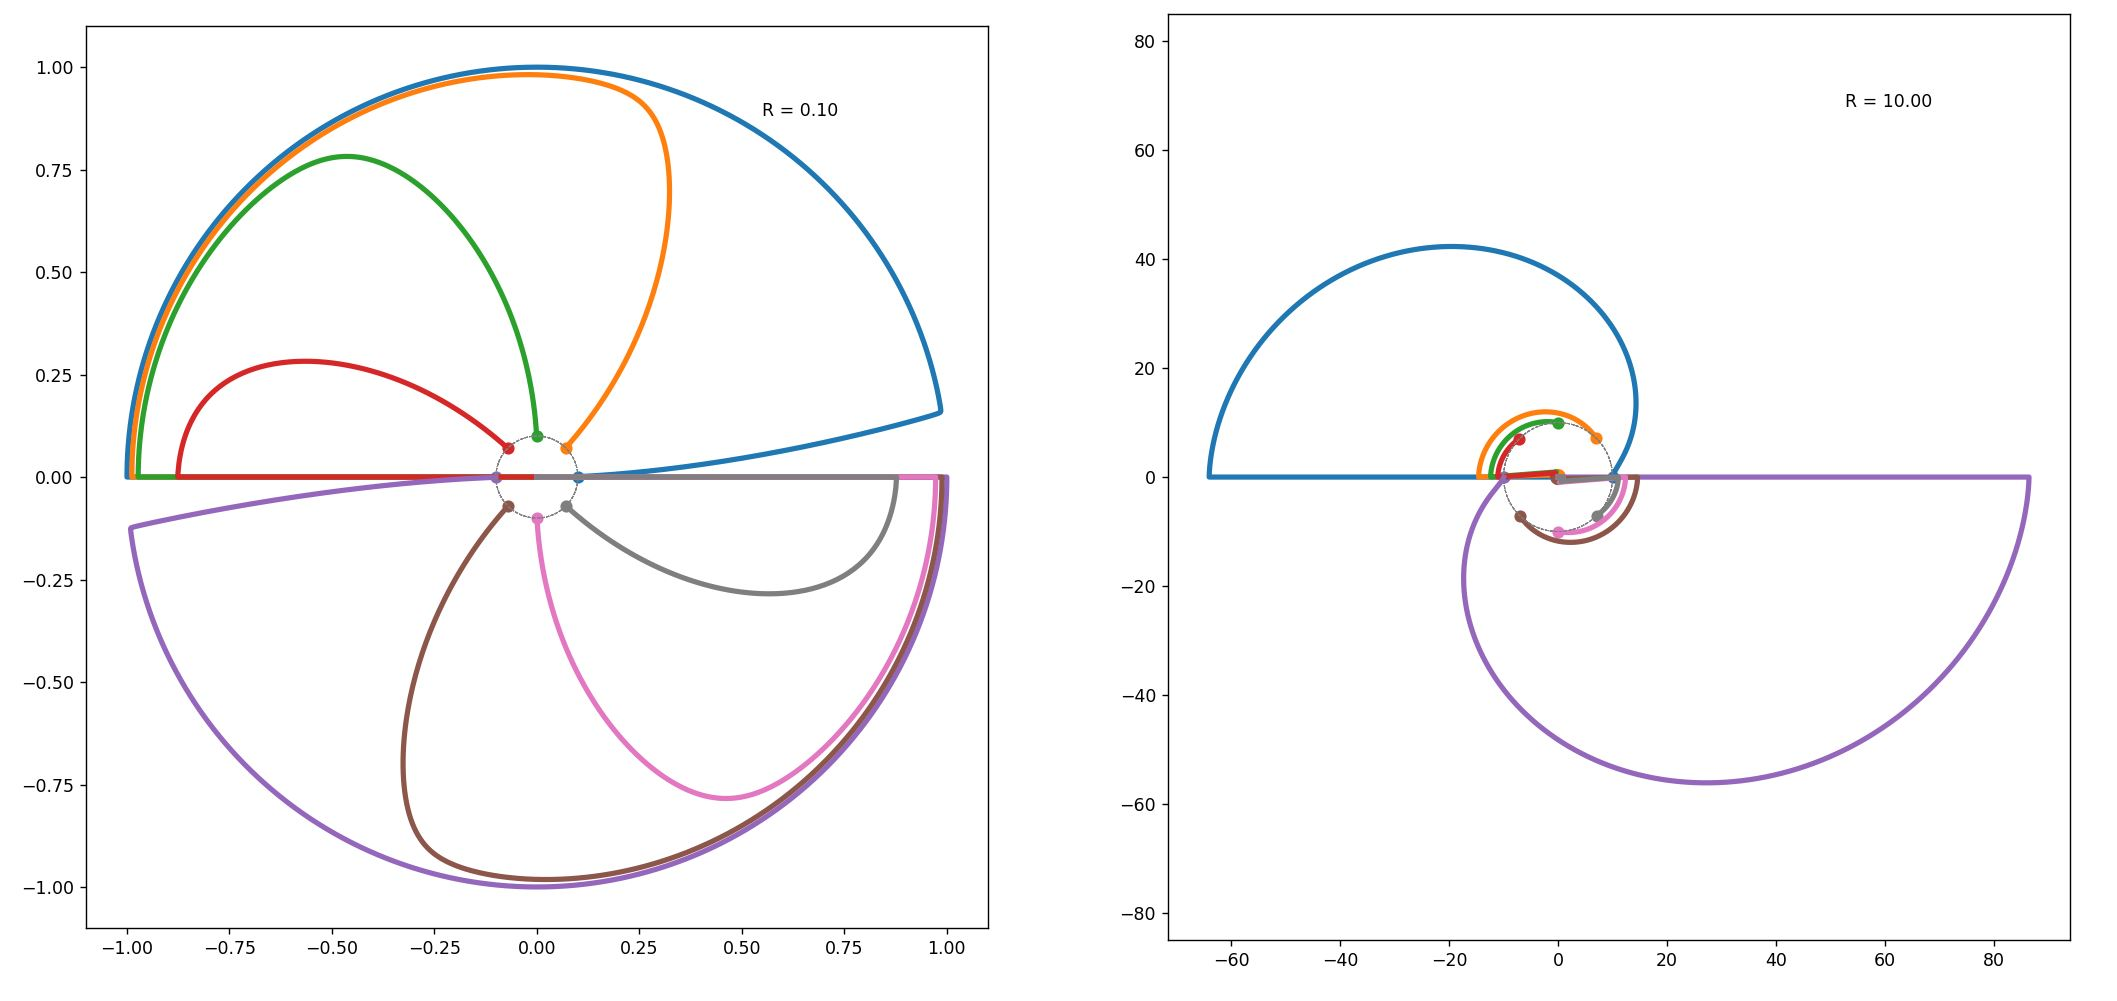
\includegraphics[scale=.2]{nullgeodesics_theta.jpg}
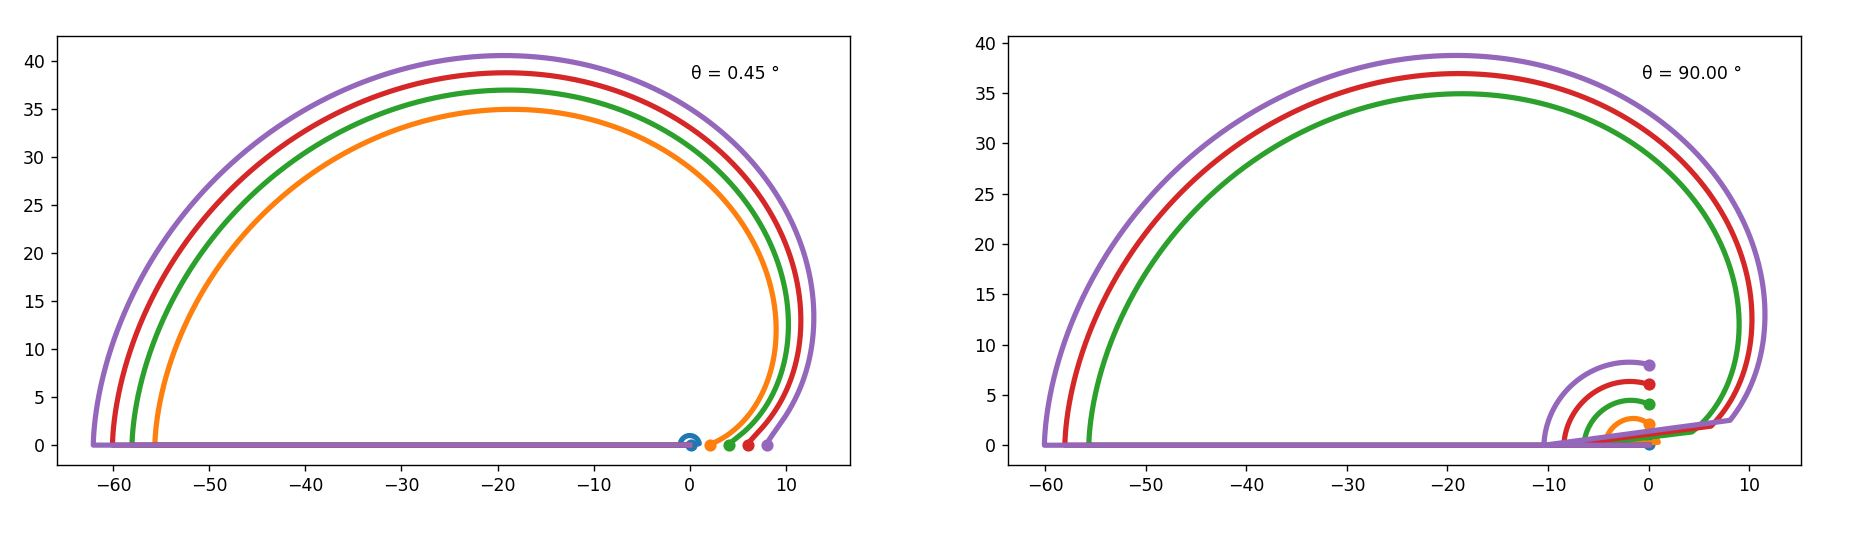
\includegraphics[scale=.25]{nullgeodesics_R.jpg}
\includegraphics[scale=.25]{nullgeodesics_theta_p.jpg}
\end{figure}
The first row shows the results for points at 2 different distance from the origin while changing the angle $\theta$. \\
The second row shows the results for points at 2 different angles  while changing the distance from the origin. \\
The second row shows the results for  a specific point while changing the the $\dv{\theta}{u}$ value in the initial condition when solving the system of differential equations. \\
Conclusion: with non-trivial metrics, getting an intuitive idea about the geodesic null lines gets very hard.
$$\blacklozenge$$
\newpage

\section{p47-exercise }
\begin{tcolorbox}
The class of all parameters $u$, for which the equations of a geodesic null line assume the simple form 2.445, are obtained from any one such parameter by linear transformation $$ \overline{u} = au + b$$ $a$ and $b$ being constants.
\end{tcolorbox}
The simple form 2.445 is :
\begin{align}
\  \dv[2]{x^r}{u} +\Gamma^r_{mn}\dv{x^m}{u}\dv{x^n}{u} = 0\\
\end{align}
The general form of a geodesic is (2.447) 
\begin{align}
\  \dv[2]{x^r}{\overline{u}} +\Gamma^r_{mn}\dv{x^m}{\overline{u}}\dv{x^n}{\overline{u}} = \lambda \dv{x^r}{\overline{u}}\\
\end{align}
So (2.447) can only of the form (2.445) if $\lambda = 0$
\begin{align}
\   \lambda  = - \frac{\dv[2]{\overline{u}}{u}}{\left( \dv{\overline{u}}{u}\right)^2} = 0\\
\end{align}
We can state that $\dv{\overline{u}}{u}\ne 0$ as $\overline{u}$ can't be a constant (being a parameter of a curve). So,
\begin{align}
\dv[2]{\overline{u}}{u}&=0\\
\Rightarrow \quad \dv{\overline{u}}{u}&=a\\
\Rightarrow \quad \overline{u}&=au +b
\end{align}
$$\blacklozenge$$
\newpage


\section{p47-exercise }
\begin{tcolorbox}
Consider a 3-space with coordinates $x,y,z$ and a metric form $\Phi = (dx)^2+(dy)^2 - (dz)^2$. prove that the geodesic null lines may be represented by the equations
$$x = au + a^,\quad y = bu + b^, \quad z = cu + c^,$$
where $u$ is a parameter and $a, a^,,b,b^,,c,c^,$ are constants which are arbitrary except for the relation $a^2+b^2-c^2 =0$.
\end{tcolorbox}
Given is 
\begin{align}
\Phi = (dx)^2+(dy)^2 - (dz)^2
\end{align}
From the previous exercise we have already proven that $x,y,z$ are of the form
\begin{align}
\ x^i = q_i u + q_i^,
\end{align}
To be a null geodesic null line we need to have (2.448)
\begin{align}
\ a_{mn}\dv{x^m}{u}\dv{x^n}{u} &=0\\
\text{from (1) we deduce}  \quad (a_{mn}) &= \begin{pmatrix}
1& 0 & 0 \\
 0&1  & 0 \\
 0&  0& -1 \\
\end{pmatrix}\\
\text{(3)}\quad\Rightarrow\quad (dx)^2+(dy)^2 - (dz)^2 &=0\\
\text{(2)}\quad\Rightarrow\quad (q_1)^2+(q_2)^2 - (q_3)^2 &=0
\end{align}
$$\blacklozenge$$
\newpage

\section{p48-exercise }
\begin{tcolorbox}
Prove that the Christoffel symbols of the first kind transform according the equation 
$$[mn,r]^, =  [pq,s]\pdv{x^p}{x^{,m}} \pdv{x^q}{x^{,n}}\pdv{x^s}{x^{,r}}+ a_{pq}\pdv{x^p}{x^{,r}}\pdv{x^q}{x^{,m}}{x^{,n}}$$
\end{tcolorbox}
From 2.438 page 45, we have
\begin{align}
\ f_r &\equiv a_{rm}\dv[2]{x^m}{u} +[mn,r]\dv{x^m}{u}\dv{x^n}{u} \quad\text{is covariant} \\
\Rightarrow\quad f_r^, &= f_s\pdv{x^s}{x^{,r}}\\
\text{with}\quad f_r^, &= a^,_{rm}\dv[2]{x^{,m}}{u} +[mn,r]^, \dv{x^{,m}}{u}\dv{x^{,n}}{u}
\end{align}
Combining (1), (2) and (3) gives 
\begin{align}
\ a^,_{rm}\dv[2]{x^{,m}}{u} +[mn,r]^, \dv{x^{,m}}{u}\dv{x^{,n}}{u} = ( a_{sm}\dv[2]{x^m}{u} +[mn,s]\dv{x^m}{u}\dv{x^n}{u})\pdv{x^s}{x^{,r}}
\end{align}
We rewrite (4) as 
\begin{align}
\ [mn,r]^, \dv{x^{,m}}{u}\dv{x^{,n}}{u} &= -\underbrace{a^,_{rm}\dv[2]{x^{,m}}{u}}_\text{(*)} +\underbrace{ a_{sm}\dv[2]{x^m}{u}\pdv{x^s}{x^{,r}}}_\text{(**)} +\underbrace{[mn,s]\dv{x^m}{u}\dv{x^n}{u}\pdv{x^s}{x^{,r}}}_\text{(***)}\\
\text{(***)} &\Leftrightarrow [mn,s]\pdv{x^m}{x^{,p}}\dv{x^{,p}}{u}\pdv{x^n}{x^{,q}}\dv{x^{,q}}{u}\pdv{x^s}{x^{,r}}
\end{align}
In (6) renaming the dummy indices $m,n,p,q$ gives
\begin{align}
\text{(***)} &\Leftrightarrow [pq,s]\pdv{x^p}{x^{,m}}\dv{x^{,m}}{u}\pdv{x^q}{x^{,n}}\dv{x^{,n}}{u}\pdv{x^s}{x^{,r}}\\
&\Leftrightarrow [pq,s]\pdv{x^p}{x^{,m}}\pdv{x^q}{x^{,n}}\pdv{x^s}{x^{,r}}\left(\dv{x^{,m}}{u}\dv{x^{,n}}{u}\right)
\end{align}
Also,
\begin{align}
\text{(**)} &\Leftrightarrow  a_{sm}\dv[2]{x^m}{u}\pdv{x^s}{x^{,r}}\\
\text{As we have also}\quad \dv[2]{x^m}{u} &= \dv{(\pdv{x^m}{x^{,p}}\dv{x^{,p}}{u})}{u}\\
&= \pdv{x^m}{x^{,p}}\dv[2]{x^{,p}}{u}+\dv{x^{,p}}{u}\pdv{x^m}{x^{,p}}{x^{,q}}\dv{x^{,q}}{u} 
\end{align}
(11) and (9) gives by changing the dummy indices ( $m\rightarrow t$, $p\rightarrow m$, $q\rightarrow n$)
\begin{align}
\text{(**)}&= \underbrace{a_{st}\pdv{x^t}{x^{,p}}\dv[2]{x^{,p}}{u}\pdv{x^s}{x^{,r}}}_\text{(****)}+a_{pq}\pdv{x^q}{x^{,m}}{x^{,n}}\pdv{x^{p}}{x^{,r}}\left(\dv{x^{,m}}{u}\dv{x^{,m}}{u}\right) \\
\text{with (****)}\quad &= a_{st}\left(\pdv{x^t}{x^{,m}}\pdv{x^s}{x^{,r}}\right)\dv[2]{x^{,m}}{u}
\end{align}
But $a_{st}$  is a covariant tensor, so
\begin{align}
\ a^{,}_{rm} &= a_{st}\pdv{x^t}{x^{,m}}\pdv{x^s}{x^{,r}}\\
\text{(13) becomes}\quad \text{(****)} &= a^{,}_{rm}\dv[2]{x^{,m}}{u}\\
\text{and from (5) we have }\quad \text{(*)} &= -a^{,}_{rm}\dv[2]{x^{,m}}{u}\\
\end{align}
and both terms cancel each other in equation (5). So adding $(*), (**)$ and $(***)$ in (5) , we get 
\begin{align}
\ [mn,r]^, \dv{x^{,m}}{u}\dv{x^{,n}}{u} &= a_{pq}\pdv{x^q}{x^{,m}}{x^{,n}}\pdv{x^{p}}{x^{,r}}\left(\dv{x^{,m}}{u}\dv{x^{,m}}{u}\right)+[pq,s]\pdv{x^p}{x^{,m}}\pdv{x^q}{x^{,n}}\pdv{x^s}{x^{,r}}\left(\dv{x^{,m}}{u}\dv{x^{,n}}{u}\right)\\
\Rightarrow \ &[mn,r]^, =[pq,s]\pdv{x^p}{x^{,m}}\pdv{x^q}{x^{,n}}\pdv{x^s}{x^{,r}}+  a_{pq}\pdv{x^{p}}{x^{,r}}\pdv{x^q}{x^{,m}}{x^{,n}}
\end{align}
$$\blacklozenge$$
\newpage

\section{p50-clarification 2.515 }
\begin{tcolorbox}
$$\dv{\left(T_rS^r\right)}{u} = \dv{T_r}{u}S^r + T_r\dv{S^r}{u} = \left(\dv{T_r}{u} - \Gamma^m_{rn}T_m\dv{x^n}{u}\right)S^r$$ with $$\frac{\delta T_r}{\delta u} = \dv{T_r}{u} -\Gamma^m_{rn}\dv{x^n}{u} T_m$$ a covariant vector.
\end{tcolorbox}
It is given that $S^r$ is a tensor propagated parallelly along the curve. The by (2.5212) we have
\begin{align}
\dv{S^r}{u} &+ \Gamma^r_{mn}S^m\dv{x^n}{u}= 0\\
\dv{S^r}{u} &= - \Gamma^r_{mn}S^m\dv{x^n}{u}\\
\text{and}\quad \dv{\left(T_rS^r\right)}{u} &= \dv{T_r}{u}S^r + T_r\dv{S^r}{u} \\
\ &= \dv{T_r}{u}S^r -\Gamma^r_{mn}S^m\dv{x^n}{u} T_r\\
\end{align}
Swap dummy indices $r$ and $m$ in the second term:
\begin{align}
\dv{\left(T_rS^r\right)}{u} &= \dv{T_r}{u}S^r -\Gamma^m_{rn}S^r\dv{x^n}{u} T_m\\
\ &= \left(\dv{T_r}{u} -\Gamma^m_{rn}\dv{x^n}{u} T_m\right)S^r\\
\end{align}
As $T_rS^r$ is an invariant and thus is also $\dv{\left(T_rS^r\right)}{u}$ and as $S^r$ can be chosen arbitrarily (as long it is a contravariant tensor), implies that $$\dv{T_r}{u} -\Gamma^m_{rn}\dv{x^n}{u} T_m$$ is covariant and thus also $$\frac{\delta T_r}{\delta u} = \dv{T_r}{u} -\Gamma^m_{rn}\dv{x^n}{u} T_m$$
$$\blacklozenge$$
\newpage

\section{p50-clarification 2.516}
\begin{tcolorbox}
$$\frac{\delta T_{rs}}{\delta u} \equiv \dv{T_{rs}}{u}  - \Gamma^m_{rn}T_{ms}\dv{x^n}{u} - \Gamma^m_{sn}T_{rm}\dv{x^n}{u}$$ is a covariant vector.
\end{tcolorbox}
We build an invariant $ T_{rs} S^rU^s$ with $S^r$ and $U^s$ arbitrary contravariant tensors. The we know that $\dv{\left( T_{rs} S^r U^s\right)}{u}$ is also an invariant. We have 
\begin{align}
\dv{\left( T_{rs} S^r U^s\right)}{u} = \dv{T_{rs}}{u} S^r U^s + T_{rs} \dv{S^r}{u} U^s + T_{rs} S^r \dv{U^s}{u}
\end{align} 
with with $S^r$ and $U^s$ propagated parallelly along the curve. Then,
\begin{align}
\dv{S^r}{u} = - \Gamma^r_{mn}S^m\dv{x^n}{u}\\
\dv{U^s}{u} = - \Gamma^s_{mn}Y^m\dv{x^n}{u}
\end{align} 
(2), (3) in (1) gives 
\begin{align}
\dv{\left( T_{rs} S^r U^s\right)}{u} = \dv{T_{rs}}{u} S^r U^s - T_{rs}U^s\Gamma^r_{mn}S^m\dv{x^n}{u} - T_{rs} S^r \Gamma^s_{mn}U^m\dv{x^n}{u}
\end{align} 
Changing the dummy indices in the second and third term gives:
\begin{align}
\dv{\left( T_{rs} S^r U^s\right)}{u} = (\dv{T_{rs}}{u}  - \Gamma^m_{rn}T_{ms}\dv{x^n}{u} - \Gamma^m_{sn}T_{rm}\dv{x^n}{u})S^r U^s
\end{align} 
As the left term is an invariant and $S^r$ and $U^s$ are arbitrary contravariant tensors, means that the expression in the brackets in the right part of the equation, is a covariant tensor.
$$\blacklozenge$$
\newpage

\section{p51-exercise}
\begin{tcolorbox}
Find the absolute derivative of $T^r_{st}$.
\end{tcolorbox}
Define the invariant $ I = D^r_{st}R^rS_sT_t$ 
\begin{align}
\ I &= D^r_{st}R^rS_sT_t\\
\Rightarrow A &= \dv{I}{u}= 
\dv{\left(D^r_{st}\right)}{u}R^rS_sT_t+
\ D^r_{st}S_sT_t\dv{\left(R^r\right)}{u}+
\ D^r_{st}R_rT_t\dv{\left(S^s\right)}{u}+
\ D^r_{st}R_rS_s\dv{\left(T^t\right)}{u}
\end{align} 
Reminder, performing a parallel propagation of a covariant and contravariant vector gives as equations
\begin{align}
\dv{V^v}{u} = - \Gamma^v_{mn}V^m\dv{x^n}{u}\\
\dv{W_w}{u} = + \Gamma^m_{wn}W^m\dv{x^n}{u}
\end{align}
So (2) becomes:
\begin{align}
\ A = \left\{ \begin{array}{c}
\dv{\left(D^r_{st}\right)}{u}R^rS_sT_t\\\\
\ -D^r_{st}S_sT_t\Gamma^r_{mn}R^m\dv{x^n}{u}\\\\
\ +D^r_{st}R_rT_t \Gamma^m_{sn}S^m\dv{x^n}{u}\\\\
\ +D^r_{st}R_rS_s\Gamma^m_{tn}T^m\dv{x^n}{u}
\end{array} \right.
\end{align}
In (5) apply the following renaming of dummy variables 
$$\left\{\begin{array}{c}
2^{nd} line: \quad r\rightarrow m, m \rightarrow r\\
3^{rd} line: \quad s\rightarrow m, m \rightarrow s\\
4^{th} line: \quad t\rightarrow m, m \rightarrow t\\
\end{array}  \right. $$
and regrouping terms with $R^rS_sT_t$,(5) becomes then
\begin{align}
\ A = \left[\dv{\left(D^r_{st}\right)}{u}+(\ D^r_{mt}\Gamma^s_{mn}+\ D^r_{sm}\Gamma^t_{mn}-\ D^m_{st}\Gamma^m_{rn})\dv{x^n}{u}\right]R^rS_sT_t
\end{align}
But $A$ is an invariant, so the expression in the square parenthesis is a tensor of the form $T^r_{st}$ and we define the absolute derivative of $T^r_{st}$ as:
$$ \frac{\delta T^r_{st}}{\delta u} = \dv{\left(T^r_{st}\right)}{u}+\Gamma^s_{mn} T^r_{mt}\dv{x^n}{u}+\Gamma^t_{mn}T^r_{sm}\dv{x^n}{u}-\Gamma^m_{rn} T^m_{st}\dv{x^n}{u}$$
$$\blacklozenge$$
\newpage

\section{p53-exercise}
\begin{tcolorbox}
Prove that $$\delta^r_{s|t} = 0, \quad a^{rs}_{|t} = 0$$
\end{tcolorbox}

i)$\delta^t_{s|t} = 0$
\begin{align}
\text{(2.524) gives:}\quad \delta^r_{s|t} &= \underbrace{\pdv{\delta^r_{s}}{x^t}}_\text{=0} + \Gamma^r_{mt}\delta^m_{s}- \Gamma^m_{st}\delta^r_{m}\\
&= \Gamma^r_{st}- \Gamma^r_{st} = 0
\end{align}

ii)$ a^{rs}_{|t} = 0$
We know that 
\begin{align}
\delta^r_{s|t} &= a_{sk}a^{kr}|_{t}\\
\Rightarrow \delta^r_{s|t} &= \pdv{a_{sk}}{x^t}a^{kr}+ a_{sk}\pdv{a^{kr} }{x^t} + \Gamma^r_{mt}a_{sk}a^{km}- \Gamma^m_{st}a_{mk}a^{kr}
\end{align}
Rearrange (4) and add $\Gamma^k_{mt}a_{ks}a^{mr}$ and subtract $\Gamma^m_{kt}a_{ms}a^{kr}$ (as $\Gamma^k_{mt}a_{ks}a^{mr} - \Gamma^m_{kt}a_{ms}a^{kr}  =0 $)
\begin{align}
\delta^r_{s|t} &= (\pdv{a_{sk}}{x^t}- \Gamma^m_{st}a_{mk}-\Gamma^m_{kt}a_{ms} )a^{kr}+ (\pdv{a^{kr} }{x^t} + \Gamma^r_{mt}a^{km}+ \Gamma^k_{mt}a^{mr})a_{sk}\\
\text{but} \quad  a_{sk|t} &= (\pdv{a_{sk}}{x^t}- \Gamma^m_{st}a_{mk}-\Gamma^m_{kt}a_{ms})\\
\text{and as (2.526)}\quad a_{sk|t} = 0\\
\text{(5) becomes}\quad \delta^r_{s|t} &= \underbrace{(\pdv{a^{kr} }{x^t} + \Gamma^r_{mt}a^{km}+ \Gamma^k_{mt}a^{mr})}_{\begin{huge}a^{kr}_{|t}\end{huge}}a_{sk}\\
\ &= a^{kr}_{|t}a_{sk}\\
\ &= 0 \quad \text{as}\quad \delta^r_{s|t}=0  \quad \text{(see first  part of this exercise)}
\end{align}
As all $a_{ks}$ can't be zero and as we didn't choose any special Riemannian space, we can conclude from $ a^{kr}_{|t}a_{sk} = 0$ that $$ a^{rs}_{|t} = 0$$ 
$$\blacklozenge$$
\newpage

\section{p54-exercise}
\begin{tcolorbox}
Prove that $$\dv{(a_{mn}\lambda^m\lambda^n)}{s} = 2 a_{mn}\lambda^m \frac{\delta\lambda^n}{\delta s}$$
\end{tcolorbox}
\begin{align} \dv{(a_{mn}\lambda^m\lambda^n)}{s}= \dv{a_{mn}}{s}\lambda^m\lambda^n+2a_{mn}\lambda^m \dv{\lambda^n}{s}
\end{align}
By definition of the absolute derivative, we have:
\begin{align}
\frac{\delta \lambda^n}{\delta s}& =\dv{\lambda ^n}{s}  + \Gamma^n_{pk}\lambda^p\dv{x^k}{s} \\
\text{(2) in (1)}\quad \dv{(a_{mn}\lambda^m\lambda^n)}{s}&= \dv{a_{mn}}{s}\lambda^m\lambda^n+2a_{mn}\lambda^m (\frac{\delta \lambda^n}{\delta s} - \Gamma^n_{pk}\lambda^p\dv{x^k}{s})\\
\ &= \dv{a_{mn}}{s}\lambda^m\lambda^n+2a_{mn}\lambda^m \frac{\delta \lambda^n}{\delta s} - 2a_{mn}\lambda^m \Gamma^n_{pk}\lambda^p\dv{x^k}{s}\\
\text{we have} \quad \Gamma^n_{pk} &= a^{ns}[pk,s]\\
\text{so,} \quad \dv{(a_{mn}\lambda^m\lambda^n)}{s}&= \dv{a_{mn}}{s}\lambda^m\lambda^n+2a_{mn}\lambda^m \frac{\delta \lambda^n}{\delta s} - 2\underbrace{a_{mn}a^{ns}}_{=\delta^s_m}[pk,s]\lambda^m \lambda^p\dv{x^k}{s}\\
&= \dv{a_{mn}}{s}\lambda^m\lambda^n+2a_{mn}\lambda^m \frac{\delta \lambda^n}{\delta s} - 2[pk,m]\lambda^m \lambda^p\dv{x^k}{s}\\
\text{but} \quad 2[pk,m]\lambda^m\lambda^p &= [pk,m]\lambda^m\lambda^p+[pk,m]\lambda^m\lambda^p\\
&= [pk,m]\lambda^m\lambda^p+[mk,p]\lambda^m\lambda^p\\
\text{we have also }\quad &\left \{ \begin{array}{c}
\ [pk,m] = \frac{1}{2}(\partial _k a_{pm} + \partial _p a_{km}-\partial _m a_{pk})\\
\ [mk,p] = \frac{1}{2}(\partial _k a_{pm} + \partial _m a_{pk}-\partial _p a_{mk})\\
\end{array}\right.\\
\ &\Rightarrow 2[pk,m] = \partial _k a_{pm}\\
\text{so} \quad \dv{(a_{mn}\lambda^m\lambda^n)}{s} &= \dv{a_{mn}}{s}\lambda^m\lambda^n - \underbrace{ \partial _k a_{pm}\dv{x^k}{s}}_{=\dv{a_{mn}}{s}} \lambda^m \lambda^p +2a_{mn}\lambda^m \frac{\delta \lambda^n}{\delta s} \\
\ & \Rightarrow \quad  \dv{(a_{mn}\lambda^m\lambda^n)}{s} = 2a_{mn}\lambda^m \frac{\delta \lambda^n}{\delta s} 
\end{align} 
$$\blacklozenge$$
\newpage

\section{p54-exercise}
\begin{tcolorbox}
Prove that $$(T^rS_s)_{|n} = T^r_{|n}S_s+T^rS_{|n}$$
\end{tcolorbox}
\begin{align} (T^rS_s)_{|n} &=  \partial_n(T^rS_s) + \Gamma^r_{nm}T^mS_s - \Gamma^m_{sn}T^rS_m\\
\ &=  \partial_n(T^r)S_s+ T^r\partial_n(S_s) + S_s\Gamma^r_{nm}T^m - T^r\Gamma^m_{sn}S_m\\
\ &=  T^r\underbrace{(\partial_n(S_s) - \Gamma^m_{sn}S_m)}_{S_{s|n}}+S_s\underbrace{(\partial_n(T^r)+ \Gamma^r_{nm}T^m)}_{T^r_{|n}}\\
\ &=  T^rS_{s|n}+S_sT^r_{|n}
\end{align}
$$\blacklozenge$$
\newpage

\section{p57-exercise}
\begin{tcolorbox}
Compute the Christoffel symbols in 2.540 directly from the definitions 2.421 and 2.422. Check that all Christoffels symbols not shown explicitly in 2.540 vanish.
\end{tcolorbox}
\textit{Easy but very tedious, not reproduced yet, later perhaps}
$$\blacklozenge$$
\newpage

\section{p57-exercise}
\begin{tcolorbox}
Show that for the spherical polar metric 2.532, we have $ln\sqrt{a} = 2 ln(x^1)+ln(sin(x^2))$ and 
$$\textbf{2.544}\quad \Gamma^n_{1n} = \frac{2}{x^1},\quad \Gamma^n_{2n} = \cot (x^2),\quad\Gamma^n_{3n} =0$$
\end{tcolorbox}
The spherical polar metric 2.532 is,
\begin{align}
\ (a_{mn})&= \begin{pmatrix}
 1& 0 & 0 \\
 0& (x^1)^2 & 0 \\
 0& 0 & (x^1 \sin (x^2))^2 \\
\end{pmatrix}\\
\Rightarrow |a_{mn}| &= \left[(x^1)^2 \sin (x^2)\right]^2\\
\Rightarrow ln(\sqrt{|a_{mn}|}) &= 2ln(x^1)+ln(\sin (x^2))\\
\Rightarrow\quad\quad &\left \{\begin{array}{c}
\Gamma^n_{1n} = \partial_1(ln(\sqrt{a})) = \frac{2}{x^1}\\\\
\Gamma^n_{2n} = \partial_2(ln(\sqrt{a})) = \frac{\cos(x^2)}{\sin(x^2)} =  \cot (x^2)\\\\
\Gamma^n_{3n} = 0\\
\end{array}\right.
\end{align} 
$$\blacklozenge$$
\newpage

\section{p58-exercise}
\begin{tcolorbox}
Show that for the spherical polar metric 
$$\textbf{2.546}\quad T^n_{\ |n} = \frac{1}{r^2}\partial_r(r^2 \ T^1) + \frac{1}{\sin \theta }\partial_{\theta}(\sin \theta\  T^2) + \partial_{\phi}T^3 $$
Obtain a similar expression for the "Laplacian" $\Delta V$ of an invariant $V$ defined as $$\textbf{2.547}\quad\Delta V = \left( a^{mn}\partial_m V\right)_{|n}$$
\end{tcolorbox}
We have
\begin{align}
\textbf{(2.545)}\quad T^n_{\ |n} &= \frac{1}{\sqrt{a}}\partial_n(\sqrt{a} \ T^n)\\
\text{and from the previous exercise p.58:}\quad \sqrt{a} &= (x^1)^2\sin(x^2)
\end{align}
\begin{align}
\Rightarrow \quad T^n_{\ |n} &= \frac{1}{\sqrt{a}}\left(\sin(x^2) \partial_1[(x^1)^2 T^1]  + (x^1)^2\partial_2 [ \sin (x^2)T^2] + (x^1)^2 \sin (x^2)\partial_3 T^3 \right)\\
&= \frac{1}{x^1} \partial_1[(x^1)^2 T^1]  + \frac{1}{\sin (x^2)}\partial_2 [ \sin (x^2)T^2] + \partial_3 T^3 
\end{align}
Replace in (4) $\quad x^1 =r$, $x^2 =  \theta$ and $x^3 = \phi$
\begin{align}
\ T^n_{\ |n} = \frac{1}{r^2} \partial_r [r^2 \ T^r]  + \frac{1}{\sin \theta}\partial_{\theta} [ \sin \theta \ T^{\theta}] + \partial_{\phi} T^{\phi} 
\end{align}
Let's calculate the Laplacian.
\begin{align}
\Delta V &= \left( a^{mn}\partial_m V\right)_{|n}\\
\text{be}\quad \quad \quad G^n &= a^{mn}\partial_m V\\
\text{then (see exercise p.32) } \quad \quad \left\{ \begin{array}{c}
\ G^1 = \partial_r V\\
\ G^2 = \frac{1}{r^2}\partial_{\theta} V\\
\ G^1 = \frac{1}{r^2 \sin ^2 \theta}\partial_{\phi} V\\
\end{array}\right.
\end{align}
and by the previous result of this exercise
\begin{align}
\Delta V &= G^n_{|n} = \frac{1}{r^2} \partial_r [r^2 \ G^1]  + \frac{1}{\sin \theta}\partial_{\theta} [ \sin \theta \ G^{2}] + \partial_{\phi} G^{3} \\
\ &= \frac{1}{r^2} \partial_r [r^2 \partial_r V]  + \frac{1}{r^2 \sin \theta}\partial_{\theta} [ \sin \theta \ \partial_{\theta} V] + \frac{1}{r^2 \sin ^2 \theta}\partial^2_{\phi} V
\end{align}
$$\blacklozenge$$
\newpage

\section{p62-exercise}
\begin{tcolorbox}
Prove that if a pair of vectors are unit orthogonal vectors at a point on a curve, and if they are both propagated parallelly along the curve, then they remain unit orthogonal vectors along the curve.
\end{tcolorbox}
Given is, a pair of vectors $U^m$ and $V^m$ which are unit orthogonal vectors at a point on a curve. So,
\begin{align}
\begin{array}{cc}
\text{U is a unit vector (2.302)}& a_{mn}U^m U^n = \epsilon\\
\text{V is a unit vector (2.302)}& a_{mn}V^m V^n = \epsilon\\
\text{U, V are orthogonal (2.317)}& a_{mn}U^m V^n = 0\\
\end{array}
\end{align}
at one point on the curve.\\
We have to prove that the above properties are valid along the curve (i.e. $\forall$ points on the curve) provided that the vectors are propagated // along the curve, which means
\begin{align}
\textbf{(2.512)}\quad\quad \frac{\delta U^r}{\delta u} &= \dv{U^r}{u} + \Gamma^r_{mn}U^m \dv{x^n}{u} = 0
\end{align}
for both vectors $U, V$. Thus,
\begin{align}
\dv{U^r}{u} = - \Gamma^r_{mn}U^m \dv{x^n}{u}
\end{align}\\
i) Consider the magnitude M at a random point on the curve
\begin{align}
\ M &= a_{mn}U^m U^n \\
\Rightarrow \quad\quad \dv{M}{s} &= \dv{a_{mn}}{u}U^m U^n + 2a_{mn}U^m \dv{U^n}{u} 
\end{align}\\
Obviously $M$ and $\dv{M}{s}$ are invariants. Also, we can choose at any point on the curve a Riemannian coordinate system (RCS) for which the Christoffel symbols vanish at that point. Hence, $\dv{U^r}{u} = 0 $ at that point and the second term in the right part of (5) vanish. (5) becomes then,
\begin{align}
 \dv{M}{s} = \pdv{a^,_{mn}}{x^{,k}}\dv{x^{,k}}{s}U^{,m} U^{,n}  
\end{align}
We also know \textbf{(2.425. page 41)} that $[km,n]^, + [kn,m]^, = \pdv{a^,_{mn}}{x^{,k}}$. But in the chosen coordinate system, $[km,n] = 0$ at the origin of this coordinate system. So by (6) we get $\dv{M}{s} = 0$.\\
So the magnitude is constant along the curve and as we know that a certain point $M =1$:\\
$$\textbf{ U,V are unit vectors along the curve}$$\newpage
ii) Consider now the angle between the vectors $U,V$. Be $A = \cos \ \theta$.By definition 
\begin{align}
\ A &= a_{mn}U ^mV^n\\
\Rightarrow \quad\quad \dv{A}{s} &= \dv{a_{mn}}{u}U^m V^n + a_{mn}(V^m \dv{U^n}{u} +U^m \dv{V^n}{u} )
\end{align}
We follow the same reasoning as in i) and so
$$\dv{A}{s} = 0$$
So, the angle is constant and we know is is $\frac{\pi}{2}$ at a certain point. So,:
$$\textbf{ U,V are orthogonal along the curve}$$

$$\blacklozenge$$
\newpage

\section{p62-exercise}
\begin{tcolorbox}
Given that $\lambda^r$ is a unit vector field, prove that $$\lambda^r_{\ |s}\lambda_r = 0 \quad \text{and}\quad \lambda^r\lambda_{r|s} = 0 $$
Is the relation $\lambda^r_{\ |s}\lambda_s = 0$ true for a general unit vector field?
\end{tcolorbox}
To simplify the calculation, we choose a random element in the unit vector field and use at that point a Riemannian coordinate system (RCS). So, we have
\begin{align}
\lambda^r_{\ |s} = \partial_s \lambda^r \quad & \text{and}\quad \lambda_{r|s} = \partial_s \lambda_r\\
\text{as we have a unit vector fields:}\quad\quad a_{mn}\lambda^m\lambda^n &= 1\\
\Leftrightarrow \lambda_n\lambda^n &= 1\quad\quad\text{(by lowering the index m)}\\
\Rightarrow \quad\quad \lambda^n\partial_s \lambda_n + \lambda_n\partial_s \lambda^n &= 0
\end{align}
We prove that $$\lambda^n\partial_s\lambda_n = \lambda_n\partial_s\lambda^n\quad \forall\text{ vector fields}$$
We have the trivial identity
\begin{align}
\partial_s(\lambda^r\lambda_r) &= \partial_s(\lambda^r\lambda_r)\\
\Leftrightarrow \quad\quad \partial_s(a^{rm}\lambda_m\lambda_r) &= \partial_s(a_{rm}\lambda^m\lambda^r)
\end{align}
\begin{lemma}: $\partial_sa^{rm} = 0$ in a Riemannian coordinate system (i.e. at the origin)\\\\
We have
\begin{align}
\ a^{rm}a_{ms} &= \delta^r_s\\
\Rightarrow a_{ms}\partial_k a^{rm}  & +a^{rm}\partial_k a_{ms} = 0\\
\text{we know (2.618)}\quad\quad \partial_r a_{mn} &= 0\quad\quad\text{at the origin of a RCS}\\
\text{so (8) becomes}\quad\quad a_{ms}\partial_k a^{rm} & = 0\\
\text{multiply (10) by}\quad a^{ns}\quad\Rightarrow \underbrace{a^{ns}a_{ms}}_{= \delta^n_m}\partial_k a^{rm}& = 0\\
\Rightarrow\quad\quad \partial_k a^{rn}& = 0
\end{align}
\end{lemma}
$$\diamond$$
Now, expanding (6) and using $\textbf{2.618}$ and the lemma:
\begin{align}
\ a^{rm}\lambda_m\partial_s \lambda_r+ a^{rm} \lambda_r \partial_s \lambda_m &= a_{rm} \lambda^m \partial_s \lambda^r + a_{rm} \lambda^r \partial_s \lambda^m\\
\text{renaming dummy indices:}\quad\quad   a^{rm} \lambda_r \partial_s \lambda_m &= a_{rm} \lambda^r \partial_s \lambda^m \\
\Rightarrow\quad\quad \lambda^m \partial_s \lambda_m &= \lambda_m \partial_s \lambda^m
\end{align}
Considering (5) and (15) we conclude:
\begin{align}
\lambda^n \partial_s \lambda_n &= \lambda_n \partial_s \lambda^n = 0
\end{align}
and as $\partial_s \lambda_n = \lambda_{n|s} $ and $\partial_s \lambda^n = \lambda^n_{\ |s} $ at the origin of the considered coordinate system, we have:
\begin{align}
\lambda^m \lambda_{n|s} &= \lambda_m \lambda^n_{\ |s} = 0
\end{align}\\
$$\diamond$$
Is the relation $\lambda^r_{|s}\lambda_s = 0$ true for a general unit vector field?\\
The answer is NO. Let's consider the following unit vector field in a Cartesian Coordinate system:
\begin{figure}[H]
\centering
\begin{minipage}[H]{.4\textwidth}
%\centering
\vspace{0pt}
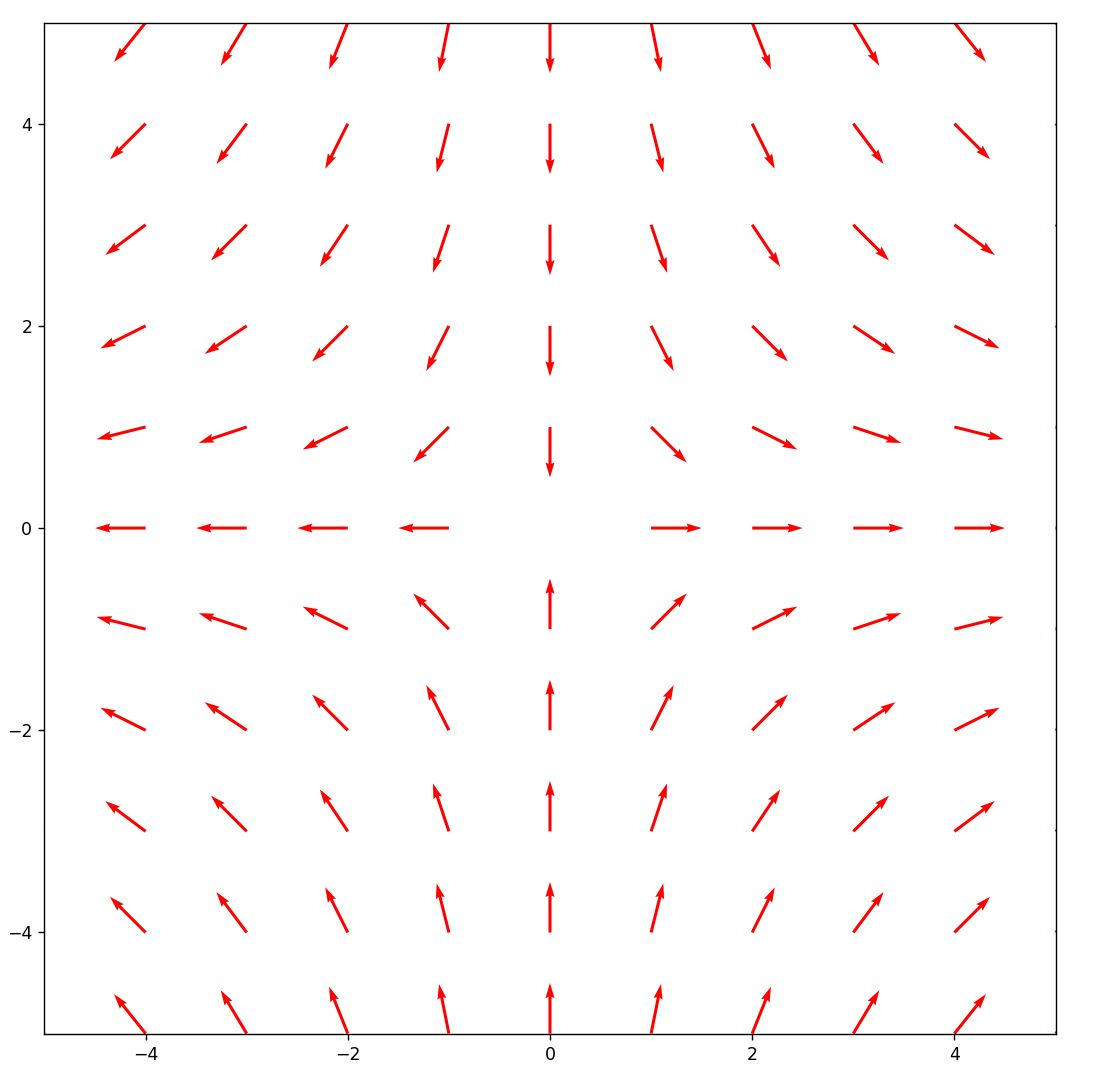
\includegraphics[scale=.3]{unitvectorfield1.jpg}
\end{minipage}\hfill
\begin{minipage}[H]{0.4\textwidth}
%\centering
\vspace{50pt}
$$V:\mathbb{R}_*^2\rightarrow \mathbb{R}^2|V(x,y) = \left< \frac{x}{\sqrt{x^2+y^2}},-\frac{y}{\sqrt{x^2+y^2}} \right>$$
\end{minipage}
\end{figure}
Put $ r = \sqrt{x^2+y^2}$, we get (as we have a Cartesian Coordinate system, the calculation simplify as the Christoffel symbols vanish and the covariant components of the vectors are equal to their contravariant part):
\begin{align}
\ & \left \{ \begin{array}{c}
\ V^1 = V_1 = +\frac{x}{r}\\
\ V^2 = V_2 = -\frac{y}{r}\\
\end{array}\right.\\
\ & \left \{ \begin{array}{cc}
\ V^1_{\ |1} =  V_{1|1} = \frac{y^2}{r^3}&V^1_{\ |2} =  V_{1|2} = -\frac{xy}{r^3}\\
\ V^2_{\ |1} =  V_{2|1} = \frac{xy}{r^3}&V^2_{\ |2} =  V_{2|2} = -\frac{x^2}{r^3}\\
\end{array}\right.\\
\Rightarrow \quad\quad &\left \{ \begin{array}{c} \  V^1_{\ |s}V_s = V^1_{\ |1}V_1+V^1_{\ |2}V_2 = \frac{y^2}{r^3}\frac{x}{r}+ (-\frac{xy}{r^3})(-\frac{y}{r}) = \frac{xy^2}{r^4} \ne 0\\
\ V^2_{\ |s}V_s = V^2_{\ |1}V_1+V^2_{\ |2}V_2 = \frac{xy}{r^3}\frac{x}{r}+ (-\frac{y}{r})(-\frac{y}{r}) = \frac{x^2 y}{r^4} \ne 0
\end{array} \right.
\end{align}
Just as a check, we calculate $V^r_{|s}V_r$ which should be zero:
\begin{align}
\Rightarrow \quad\quad &\left \{ \begin{array}{c}V^s_{\ |1}V_s = V^1_{\ |1}V_1+V^2_{\ |1}V_2 = (+\frac{y^2}{r^3})\frac{x}{r}+ (+\frac{xy}{r^3})(-\frac{y}{r}) =0\\
\ V^s_{\ |2}V_s = V^1_{\ |2}V_1+V^2_{\ |2}V_2 = (-\frac{xy}{r^3})\frac{x}{r}+ (-\frac{y}{r})(-\frac{x^2}{r^3}) = 0
\end{array} \right.
\end{align}\\\\
Now, let's consider another unit vector field in a Cartesian Coordinate system:
\begin{figure}[H]
\centering
\begin{minipage}[H]{.4\textwidth}
%\centering
\vspace{0pt}
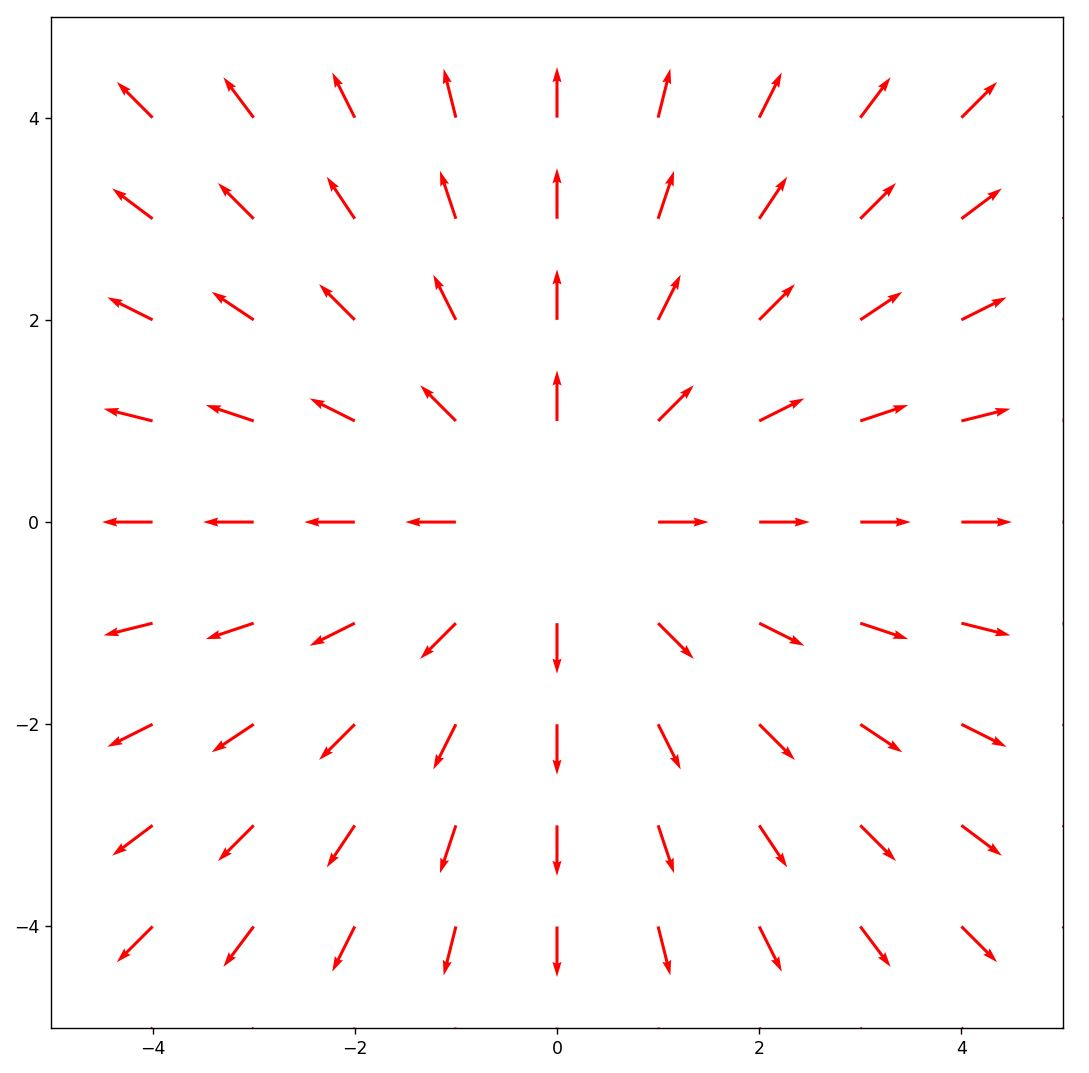
\includegraphics[scale=.3]{unitvectorfield2.jpg}
\end{minipage}\hfill
\begin{minipage}[H]{0.4\textwidth}
%\centering
\vspace{50pt}
$$V:\mathbb{R}_*^2\rightarrow \mathbb{R}^2|V(x,y) = \left< \frac{x}{\sqrt{x^2+y^2}},\frac{y}{\sqrt{x^2+y^2}} \right>$$
\end{minipage}
\end{figure}
\begin{align}
\ & \left \{ \begin{array}{c}
\ V^1 = V_1 = +\frac{x}{r}\\
\ V^2 = V_2 = +\frac{y}{r}\\
\end{array}\right.\\
\ & \left \{ \begin{array}{cc}
\ V^1_{\ |1} =  V_{1|1} = \frac{y^2}{r^3}&V^1_{\ |2} =  V_{1|2} = -\frac{xy}{r^3}\\
\ V^2_{\ |1} =  V_{2|1} = -\frac{xy}{r^3}&V^2_{\ |2} =  V_{2|2} = +\frac{x^2}{r^3}\\
\end{array}\right.\\
\Rightarrow \quad\quad &\left \{ \begin{array}{c} \  V^1_{\ |s}V_s = V^1_{\ |1}V_1+V^1_{\ |2}V_2 = (+\frac{y^2}{r^3})\frac{x}{r}+ (-\frac{xy}{r^3})(+\frac{y}{r}) =  0\\
\ V^2_{\ |s}V_s = V^2_{\ |1}V_1+V^2_{\ |2}V_2 = (-\frac{xy}{r^3})\frac{x}{r}+ (+\frac{y}{r})(+\frac{y}{r}) =  0
\end{array} \right.
\end{align}
Just as a check, we calculate $V^r_{|s}V_r$ which should be zero:
\begin{align}
\Rightarrow \quad\quad &\left \{ \begin{array}{c}V^s_{\ |1}V_s = V^1_{\ |1}V_1+V^2_{\ |1}V_2 = (+\frac{y^2}{r^3})(+\frac{x}{r})+ (-\frac{xy}{r^3})(+\frac{y}{r}) =0\\
\ V^s_{\ |2}V_s = V^1_{\ |2}V_1+V^2_{\ |2}V_2 = (-\frac{xy}{r^3})(+\frac{x}{r})+ (+\frac{y}{r})+\frac{x^2}{r^3}) = 0
\end{array} \right.
\end{align}\\
So, in the second example the relationship $\lambda^r_{|s}\lambda_s = 0$ holds.
Question (to investigate further and later) : does the fact that in the first case $\grad \maal \overline{V}  \ne 0$ and in the second case $\grad \maal \overline{V}= 0$, means that there is some relation with this expression?
$$\blacklozenge$$
\newpage

\section{p64-clarification 2.625}
\begin{tcolorbox}
$\textbf{2.625} \quad\quad\quad\quad\quad\quad \dv{ x^r}{x^N} = \frac{X^r}{X^N}$
\end{tcolorbox}
Be $C$ a surface defined by the function $F(x^1,\dots, x^{N-1}) = C$ and  $c_{\perp}$ the curve intersecting the surface $C$ perpendicularly at a point $p$.\\
Along the curve at that point $p$ we have
\begin{align}
\text{as}\quad\quad & \left \{ \begin{array}{cc}
\dv{ x^r}{s}& \text{is the tangent vector along}\quad c_{\perp}\\
\ X^r = a^{rn}\pdv{F}{x^n}& \text{ is orthogonal on the surface (2.623)}\quad C\\
\end{array}\right.\\
\Rightarrow \quad\quad & \dv{ x^r}{s} = kX^r
\end{align}
So, $\dv{ x^r}{s}$ is proportional to $X^r$ (as the curve intersects the surface orthogonally). This means that also all the components (coordinates) of both quantities are proportional. And so,
\begin{align}
\frac{\dv{ x^r}{s}}{\dv{ x^N}{s}} &= \frac{kX^r}{kX^N}\\
\Rightarrow\quad\quad \dv{ x^r}{x^N} &= \frac{X^r}{X^N}
\end{align}
$$\blacklozenge$$
\newpage

\section{p65-exercise}
\begin{tcolorbox}
Deduce from $\textbf{2.629}$ that $$a^{N \rho} = 0  \quad\quad a^{NN} = \frac{1}{a_{NN}}$$
\end{tcolorbox}
We have (see 2.629):
\begin{align}
\ a_{N\rho} =0\\
\text{and also}\quad\quad a_{Nm}a^{ms} = \delta^s_N
\end{align}
In (2) split the $m$ index in the subspace and the remaining coordinate $N$
\begin{align}
\ a_{N\rho}a^{\rho s} +  a_{NN}a^{N s} &= \delta^s_N\\
\text{as}\quad a_{N\rho} =0 \Rightarrow \quad\quad a_{NN}a^{N s} &= \delta^s_N
\end{align}\\
Case 1: $s\ne N$
\begin{align}
\  a_{NN}a^{N s} =0 \quad \Leftrightarrow \quad a_{NN}a^{N \rho} =0 \quad\quad \text{(as}\quad s\ne N \text{)}\\
\text{as we suppose}\quad a_{NN}\ne 0 \quad \Rightarrow \quad a^{N \rho} =0
\end{align}\\

Case 2: $s= N$
\begin{align}
\  a_{NN}a^{N N} &=1 \\
\Rightarrow \quad a^{N N} &=\frac{1}{a_{NN}}
\end{align}
$$\blacklozenge$$
\newpage


\section{p69-clarification on 2.645}
\begin{tcolorbox}
In 2.645 we have $$T_{\alpha | \beta} =T_{\alpha || \beta}  +\frac{1}{2}\frac{1}{a_{NN}}\partial_N  a_{\alpha\beta}T_{N}$$ and $$T_{\alpha | \beta} =T_{\alpha || \beta}  +\frac{1}{2}\partial_N  a_{\alpha\beta}T^{N}$$
\end{tcolorbox}
Indeed,
\begin{align}
\ T^N &= a^{mN}T_m\\
\ & = a^{\alpha N}T_{\alpha}+a^{N N}T_{N}\\
\text{but (2.631)}\quad\quad a^{\alpha N} &= 0\\
\Rightarrow \quad\quad T^N &= a^{NN} T_N\\
\text{as}\quad a^{NN}= \frac{1}{a_{NN}} \quad \Rightarrow \quad\quad  T_{\alpha | \beta} &= T_{\alpha || \beta}  + \frac{1}{2}\partial_N  a_{\alpha\beta}T^{N}
\end{align}
$$\blacklozenge$$
\newpage
\section{p69-exercise}
\begin{tcolorbox}
Show that
$$\textbf{2.648}\quad\quad T^{\alpha}_{\ |\beta} = T^{\alpha}_{\ ||\beta} + \half a^{\alpha \mu} \partial_N a_{\mu\beta}T^N$$
$$\textbf{2.649}\quad\quad T^{N}_{\ |\alpha} = \partial_{\alpha}T^{N} - \frac{1}{2 a_{NN}} \partial_N a_{\alpha\mu}T^{\mu} + \frac{1}{2 a_{NN}} \partial_{\alpha} a_{NN}T^{N}$$
$$\textbf{2.650}\quad\quad T^{\alpha}_{\ |N} = \partial_{N}T^{\alpha}  + \half a^{\alpha\mu} \partial_N a_{\mu\sigma}T^{\sigma} - \half a^{\alpha\mu}  \partial_{\mu} a_{NN}T^{N}$$
\end{tcolorbox}
i) $T^{\alpha}_{\ |\beta} = T^{\alpha}_{\ ||\beta} + \half a^{\alpha \mu} \partial_N a_{\mu\beta}T^N$\\
\begin{align}
\textbf{(2.520)}\quad\quad \Rightarrow \quad\quad T^{\alpha}_{\ |\beta} &= \partial_{\beta}T^{\alpha}+\Gamma^{\alpha}_{m\beta}T^m \quad\quad\text{(}m = 1,\dots,N \text{)}\\
\Leftrightarrow \quad\quad T^{\alpha}_{\ |\beta} &= \underbrace{ \partial_{\beta}T^{\alpha}+ \Gamma^{\alpha}_{\mu \beta} T^{\mu}}_{T^{\alpha}_{ \ || \beta}} +\Gamma^{\alpha}_{N \beta}T^{N}\\
\textbf{(2.639)}\quad\quad \Gamma^{\alpha}_{N\beta} &= \half a^{\alpha \mu}\partial_N a^{\mu \beta}\\
\text{(2) and (3): }\quad\quad T^{\alpha}_{\ |\beta} &= T^{\alpha}_{\ ||\beta} + \half a^{\alpha \mu} \partial_N a_{\mu\beta}T^N
\end{align}
$$\diamond$$
Remark: We also use $\textbf{(2.639)}$ for the two other identities.\\\\
ii) $T^{N}_{\ |\alpha} = \partial_{\alpha}T^{N} - \frac{1}{2 a_{NN}} \partial_N a_{\alpha\mu}T^{\mu} + \frac{1}{2 a_{NN}} \partial_{\alpha} a_{NN}T^{N}$\\
\begin{align}
\textbf{(2.520)}\quad\quad \Rightarrow \quad\quad T^{N}_{\ |\alpha} &= \partial_{\alpha}T^{N}+\Gamma^{N}_{m\alpha}T^m \quad\quad\text{(}m = 1,\dots,N \text{)}\\
\Leftrightarrow \quad\quad T^{N}_{\ |\alpha} &=  \partial_{\beta}T^{\alpha}+ \underbrace{\Gamma^{N}_{\sigma \alpha}}_{ - \frac{1}{2a_{NN}}\partial_N a_{\sigma\alpha}} T^{\sigma } +\underbrace{\Gamma^{N}_{N \alpha}}_{ \frac{1}{2a_{NN}}\partial_{\alpha} a_{NN}}T^{N}\\
\Rightarrow \quad\quad T^{N}_{\ |\alpha} &=  \partial_{\beta}T^{\alpha} - \frac{1}{2a_{NN}}\partial_N a_{\sigma\alpha}T^{\sigma } +\frac{1}{2a_{NN}}\partial_{\alpha} a_{NN}T^{N}
\end{align}\\
iii) $T^{\alpha}_{\ |N} = \partial_{N}T^{\alpha}  + \half a^{\alpha\mu} \partial_N a_{\mu\sigma}T^{\sigma} - \half a^{\alpha\mu}  \partial_{\mu} a_{NN}T^{N}$\\
\begin{align}
\textbf{(2.520)}\quad\quad \Rightarrow \quad\quad T^{\alpha}_{\ |N} &= \partial_{N}T^{\alpha}+\Gamma^{\alpha}_{mN}T^m \quad\quad\text{(}m = 1,\dots,N \text{)}\\
\Leftrightarrow \quad\quad T^{\alpha}_{\ |N} &=  \partial_{N}T^{\alpha}+ \underbrace{\Gamma^{\alpha}_{\sigma N }}_{ \half a^{\alpha \mu}\partial_N a_{\mu\sigma}}  T^{\sigma }+\underbrace{\Gamma^{\alpha}_{N N}}_{ -\half a^{\alpha\mu}\partial_{\mu} a_{NN}}T^{N}\\
\Rightarrow \quad\quad T^{\alpha}_{\ |N} &=  \partial_{N}T^{\alpha}+ \half a^{\alpha \mu}\partial_N a_{\mu\sigma}T^{\sigma } -\half a^{\alpha\mu}\partial_{\mu} a_{NN}T^{N}
\end{align}
$$\blacklozenge$$
\newpage

\section{p71-exercise}
\begin{tcolorbox}
Write down equation 2.643 tot 2.650 for the special cae of a geodesic normal coordinate system.
\end{tcolorbox}
\begin{align}
\ \textbf{(2.643)}\quad \quad T_{\alpha || \beta} &= \partial_{\beta}T_{\alpha} - \Gamma^{\gamma}_{\alpha\beta}T_{\gamma}\quad\quad \text{(does not change)}\\
\textbf{(2.644)}\quad \quad T_{\alpha | \beta} &=T_{\alpha || \beta}  - \underbrace{\Gamma^{N}_{\alpha\beta}}_{=\frac{1}{2} \frac{1}{a_{NN}}\partial_N  a_{\alpha\beta}}T_{N}\\
&=T_{\alpha || \beta}  +\frac{1}{2} \epsilon\partial_N  a_{\alpha\beta}T_{N}\\
\textbf{(2.645)}\quad \quad T_{\alpha | \beta} &=T_{\alpha || \beta}  +\frac{1}{2}\partial_N  a_{\alpha\beta}T^{N}\quad\quad \text{(does not change)}\\
\textbf{(2.646)}\quad \quad T_{N| \alpha } &=\partial_{\alpha}T_N  -\frac{1}{2}\partial_N  a_{\mu\alpha}T^{\mu} -\frac{1}{2}\underbrace{\partial_{\alpha}  a_{NN}}_{=0}T^{N}\\
&=\partial_{\alpha}T_N  -\frac{1}{2}\partial_N  a_{\mu\alpha}T^{\mu} \\
\textbf{(2.647)}\quad \quad T_{ \alpha |N } &=\partial_N T_{\alpha}  -\frac{1}{2}\partial_N  a_{\mu\alpha}T^{\mu} -\frac{1}{2}\underbrace{\partial_{\alpha}  a_{NN}}_{=0}T^{N}\\
&=\partial_N T_{\alpha}  -\frac{1}{2}\partial_N  a_{\mu\alpha}T^{\mu} \\
\textbf{(2.648)}\quad \quad T^{\alpha}_{ \  | \beta} &=T^{\alpha}_{ || \beta}  + \frac{1}{2}a^{\alpha\mu}\partial_N  a_{\mu\beta}T_{N}\quad\quad\text{(does not change)}\\
\textbf{(2.649)}\quad \quad T^N_{ \ | \alpha} &=\partial_{\alpha}T^N  -\frac{1}{2}\frac{1}{a_{NN}}\partial_N  a_{\mu\alpha}T^{\mu} -\frac{1}{2}\frac{1}{a_{NN}}\underbrace{\partial_{\alpha}  a_{NN}}_{=0}T^{N}\\
\ &= \partial_{\alpha}T^N  -\frac{1}{2}\epsilon\partial_N  a_{\mu\alpha}T^{\mu} \\
\textbf{(2.650)}\quad \quad T^{\alpha}_{\ |N} &=\partial_N T^{\alpha}  +\frac{1}{2}a^ {\alpha\mu}\partial_N  a_{\mu\sigma}T^{\sigma} -\frac{1}{2}a^{\alpha\mu}\underbrace{\partial_{\mu}  a_{NN}}_{=0}T^{N}\\
\ &=\partial_N T^{\alpha}  +\frac{1}{2}a^ {\alpha\mu}\partial_N  a_{\mu\sigma}T^{\sigma} 
\end{align}
\\\\
To investigate: note (3) and (4) which suggest that $\epsilon T_{N} = T^{N}$. Prove formally?
$$\blacklozenge$$
\newpage


\section{p73-Clarification 2.706}
\begin{tcolorbox}
... Let us now define a unit vector $\lambda^r_{(2)}$ and a positive invariant $\kappa_{(2)}$ by the equation \\
\begin{align}
\left \{ \begin{array}{c}
\frac{\delta\lambda_{(1)}^r}{\delta s} = \kappa_{(2)}\lambda^r_{(2)} - \epsilon\epsilon_{(1)}\kappa_{(1)}\lambda^r\\
\epsilon_{(2)}\lambda^n_{(2)}\lambda_{(2)n} = 1
\end{array} \right.
\end{align}  
\end{tcolorbox}
We can state that $\kappa_{(2)}$ is an invariant but one has to check whether the expression $(1)$ implies that $\kappa_{(2)}$ is indeed invariant.\\
What we know is that $\lambda^r, \frac{\delta \lambda^r}{\delta s},\frac{\delta\lambda_{(1)}^r}{\delta s},  \lambda^r_{(2)}$ are contravariant vectors. Also $\kappa_{(1)}$ is an invariant as $\frac{\delta\lambda^r}{\delta s} = \kappa_{(1)}\lambda^r_{(1)}$ and the magnitude of $\frac{\delta\lambda^r}{\delta s}$ does not depend on the coordinate system. So,
\begin{align}
\text{(1)}\times \lambda_{(2)r} \quad\Rightarrow \quad\quad \frac{\delta\lambda_{(1)}^r}{\delta s}\lambda_{(2)r} &= \kappa_{(2)}\lambda^r_{(2)}\lambda_{(2)r} - \epsilon\epsilon_{(1)}\kappa_{(1)}\lambda^r\lambda_{(2)r}\\
\Rightarrow \quad\quad \kappa_{(2)}\underbrace{\lambda^r_{(2)}\lambda_{(2)r}}_{\text{invariant}} &= \underbrace{\frac{\delta\lambda_{(1)}^r}{\delta s}\lambda_{(2)r}}_{\text{invariant}}  + \underbrace{\epsilon\epsilon_{(1)}}_{\text{invariant}} \underbrace{\kappa_{(1)}}_{\text{invariant}} \underbrace{\lambda^r \lambda_{(2)r}}_{\text{invariant}} \\
\Rightarrow \quad\quad \kappa_{(2)}&= \text{invariant} 
\end{align}
$$\blacklozenge$$
\newpage

\section{p74-Clarification 2.710}
\begin{tcolorbox}
\begin{align}
\textbf{2.710}\quad\quad\left \{ \begin{array}{c}
\frac{\delta\lambda_{(M-1)}^r}{\delta s} = \kappa_{(M)}\lambda^r_{(M)} - \epsilon_{(M-2)}\epsilon_{(M-1)}\kappa_{(M-1)}\lambda^r_{(M-2)}\\
\epsilon_{(M-1)}\lambda^n_{(M-1)}\lambda_{(M-1)n} = 1\quad\quad \text{(M=1,2,...,N)}
\end{array} \right.
\end{align}
... It is easily proved by mathematical induction that the whole sequence of vectors defined by 2.710 are perpendicular to the tangent and to one another ...
\end{tcolorbox}
We already know from 2.703 to 2.709 that $\lambda^r, \lambda_{(1)}^r,\lambda_{(2)}^r,\lambda_{(3)}^r$, satisfying equations (1), are all mutually perpendicular. Let us assume that the orthogonality for the set $\{\lambda_{(k)}^r:k= 0,1,2,3,..., M-1\}$ has been verified. We prove by induction that then, $\lambda_{(M)}^r$ will be orthogonal to all elements of the set.\\
i) Consider the set $\{\lambda_{(k)}^r:k= 0,1,2,3,..., M-3\}$ where we already know that $\lambda_{(k)}^r$ are mutually perpendicular and also $\lambda_{(k)}^r \perp \lambda_{(M-1)}^r $, $\lambda_{(k)}^r \perp \lambda_{(M-2)}^r$ and $\lambda_{(M-1)}^r \perp \lambda_{(M-1)}^r \quad \forall k$.
\begin{align}
\text{(1)}\times \lambda_{(k)r}\quad\Rightarrow\quad\quad \frac{\delta\lambda_{(M-1)}^r}{\delta s}\lambda_{(k)r} &= \kappa_{(M)}\lambda^r_{(M)}\lambda_{(k)r} - \epsilon_{(M-2)}\epsilon_{(M-1)}\kappa_{(M-1)}\underbrace{\lambda^r_{(M-2)}\lambda_{(k)r}}_{=0}\\
\text{We have}  \quad \quad\quad\quad\quad\lambda_{(k)r}\lambda^r_{(M-1)} &=0\\
\Rightarrow \quad \quad\quad\quad\quad\ \frac{\delta\lambda_{(k)r}\lambda_{(M-1)}^r}{\delta s} &= \lambda_{(M-1)}^r\frac{\delta\lambda_{(k)r}}{\delta s}+\lambda_{(k)r}\delta\frac{\lambda_{(M-1)}^r}{\delta s}=0\\
\Rightarrow \quad \quad\quad\quad\quad\ \lambda_{(k)r}\delta\frac{\lambda_{(M-1)}^r}{\delta s} &= - \lambda_{(M-1)}^r\frac{\delta\lambda_{(k)r}}{\delta s}\\
\text{We have}\quad \quad\quad\quad\quad\frac{\delta\lambda_{(k)r}}{\delta s} &= \kappa_{(k+1)}\lambda_{(k+1)r} - \epsilon_{(k)}\epsilon_{(k-1)}\kappa_{(k)}\lambda_{(k-1)r}\\
\text{(5) and (6)}\Rightarrow \quad \quad\quad\quad\quad\ \lambda_{(k)r}\delta\frac{\lambda_{(M-1)}^r}{\delta s} &= -\kappa_{(k+1)}\underbrace{\lambda_{(k+1)r} \lambda_{(M-1)}^r}_{=0} - \epsilon_{(k)}\epsilon_{(k-1)}\kappa_{(k)}\underbrace{\lambda_{(k-1)r}\lambda_{(M-1)}^r}_{=0}\\
\text{From (2)}\Rightarrow \quad \quad\quad\quad\quad\ \kappa_{(M)}\lambda^r_{(M)}\lambda_{(k)r}&=0\\
\Rightarrow \quad \quad\quad\quad\quad\ \lambda^r_{(M)}& \perp\lambda_{(k)r}\quad\quad \forall k= 0,1,2,3,..., M-3 
\end{align}\\\\
ii) Consider the case $k = M-1$\\\begin{align}
\text{(1)}\times \lambda_{(M-1)r}\quad \frac{\delta\lambda_{(M-1)}^r}{\delta s}\lambda_{(M-1)r} &= \kappa_{(M)}\lambda^r_{(M)}\lambda_{(M-1)r} - \epsilon_{(M-2)}\epsilon_{(M-1)}\kappa_{(M-1)}\underbrace{\lambda^r_{(M-2)}\lambda_{(M-1)r}}_{=0}\\
\text{from (2.530):}\quad\quad \frac{\delta\lambda_{(M-1)}^r}{\delta s}\lambda_{(M-1)r}  &= \half\underbrace{\frac{\delta\lambda_{(M-1)r}\lambda_{(M-1)}^r}{\delta s}}_{=0\text{ as }\lambda_{(M-1)r}\lambda_{(M-1)}^r =  \epsilon_{(M-1)}}\\
\Rightarrow \quad \quad\quad\quad\quad \kappa_{(M)}\lambda^r_{(M)}\lambda_{(M-1)r}&=0\\
\Rightarrow \quad \quad\quad\quad\quad \lambda_{(M-1)r} & \perp\lambda_{(M)r}
\end{align}

iii) Consider the case $k = M-2$\\\begin{align}
\text{(1)}\times \lambda_{(M-2)r}\quad \frac{\delta\lambda_{(M-1)}^r}{\delta s}\lambda_{(M-2)r} &= \kappa_{(M)}\lambda^r_{(M)}\lambda_{(M-2)r} - \epsilon_{(M-2)}\epsilon_{(M-1)}\kappa_{(M-1)}\underbrace{\lambda^r_{(M-2)}\lambda_{(M-2)r}}_{=\epsilon_{(M-2)}}\\
\Rightarrow \quad \quad\quad\quad\quad\frac{\delta\lambda_{(M-1)}^r}{\delta s}\lambda_{(M-2)r} &= \kappa_{(M)}\lambda^r_{(M)}\lambda_{(M-2)r} - \epsilon_{(M-1)}\kappa_{(M-1)}\underbrace{\epsilon_{(M-2)}\epsilon_{(M-2)}}_{=1}\\
\Rightarrow \quad \quad\quad\quad\quad\frac{\delta\lambda_{(M-1)}^r}{\delta s}\lambda_{(M-2)r} &= \kappa_{(M)}\lambda^r_{(M)}\lambda_{(M-2)r} - \epsilon_{(M-1)}\kappa_{(M-1)}\\
\text{We have}  \quad \quad\quad\quad\quad\lambda_{(M-1)}^r\lambda_{(M-2)r} &=0\\
\Rightarrow \quad \quad\quad\quad\quad\ \lambda_{(M-2)r}\frac{\delta\lambda_{(M-1)}^r}{\delta s} &= -\lambda_{(M-1)}^r\frac{\delta\lambda_{(M-2)r}}{\delta s}\\
\text{We have also }  \quad\frac{\delta\lambda_{(M-2)r}}{\delta s} &= \kappa_{(M-1)}\lambda_{(M-1)r} - \epsilon_{(M-3)}\epsilon_{(M-2)}\kappa_{(M-2)}\lambda_{(M-3)r}\\
\text{(19)}\times \lambda^r_{(M-1)} \text{ and (18): }  \lambda_{(M-2)r}\frac{\delta\lambda_{(M-1)}^r}{\delta s} &= -\kappa_{(M-1)}\underbrace{\lambda^r_{(M-1)}\lambda_{(M-1)r}}_{=\epsilon_{(M-1)}} - \epsilon_{(M-3)}\epsilon_{(M-2)}\kappa_{(M-2)}\underbrace{\lambda^r_{(M-3)}\lambda_{(M-1)r}}_{=0}\\
\Rightarrow \quad \quad\quad\quad\quad\ \lambda_{(M-2)r}\frac{\delta\lambda_{(M-1)}^r}{\delta s} &= -\kappa_{(M-1)}\epsilon_{(M-1)}\\
\text{(16) and (21):}\quad \quad\quad\quad\quad -\kappa_{(M-1)}\epsilon_{(M-1)} &= \kappa_{(M)}\lambda^r_{(M)}\lambda_{(M-2)r} - \epsilon_{(M-1)}\kappa_{(M-1)}\\
\Rightarrow \quad \quad\quad\quad\quad \kappa_{(M)}\lambda^r_{(M)}\lambda_{(M-2)r}&=0\\
\Rightarrow \quad \quad\quad\quad\quad \lambda_{(M-2)r}\perp\lambda_{(M)r}
\end{align}
With, i), ii), iii) all possible cases are covered which makes the proof complete.
$$\blacklozenge$$
\newpage

\section{p75-Clarification 2.714}
\begin{tcolorbox}
$\textbf{2.714} \quad \quad (\kappa_{(1)})^2 = \epsilon_{(1)} a_{mn} \frac{\delta \lambda^{m}}{\delta s} \frac{\delta \lambda^{n}}{\delta s}$,   $\quad \quad \epsilon_{(1)} = \pm 1$
\end{tcolorbox}
\begin{align}
\ \frac{\delta \lambda^{n}}{\delta s} &= \kappa_{(1)}\lambda_{(1)}^{n}\\
\text{(1)}\times \text{(1)}\quad\Rightarrow \quad\quad \frac{\delta \lambda^{m}}{\delta s}\frac{\delta \lambda^{n}}{\delta s} &= (\kappa_{(1)})^2 \lambda_{(1)}^{m}\lambda_{(1)}^{n}\\
\text{(2)}\times a_{mn} \Rightarrow\quad\quad a_{mn}\frac{\delta \lambda^{m}}{\delta s}\frac{\delta \lambda^{n}}{\delta s} &= a_{mn}(\kappa_{(1)})^2 \lambda_{(1)}^{m}\lambda_{(1)}^{n}\\
\ &= (\kappa_{(1)})^2 \underbrace{\lambda_{(1)m} \lambda_{(1)}^{n}}_{=\epsilon_{(1)}}\\
\ &= (\kappa_{(1)})^2 
\end{align}
$$\blacklozenge$$
\newpage


\section{p75-exercise}
\begin{tcolorbox}
For positive definite metric forms, write out explicitly the Frenet formulae for the case N=2, 3 and 4.
\end{tcolorbox}
The general Frenet formulae are 
\begin{align}
\left \{ \begin{array}{c}
\frac{\delta\lambda_{(M-1)}^r}{\delta s} = \kappa_{(M)}\lambda^r_{(M)} - \epsilon_{(M-2)}\epsilon_{(M-1)}\kappa_{(M-1)}\lambda^r_{(M-2)}\\
\epsilon_{(M-1)}\lambda^n_{(M-1)}\lambda_{(M-1)n} = 1\quad\quad \text{(M=1,2,...,N)}
\end{array} \right.
\end{align}
As $\Phi$ is positive definite, we have $\epsilon_{(k)} = 1\quad \forall k$
\begin{center}
\begin{tabular}{ |c|c|c|c| } 
\hline
N=2 & N=3 & N=4 \\
\hline
& &\\
$\frac{\delta\lambda^r}{\delta s} = \kappa_{(1)}\lambda^r_{(1)} $ & $\frac{\delta\lambda^r}{\delta s} = \kappa_{(1)}\lambda^r_{(1)} $& $\frac{\delta\lambda^r}{\delta s} = \kappa_{(1)}\lambda^r_{(1)} $ \\ 
$\frac{\delta\lambda_{(1)}^r}{\delta s} = \kappa_{(2)}\lambda^r_{(2)} - \kappa_{(1)}\lambda^r$& $\frac{\delta\lambda_{(1)}^r}{\delta s} = \kappa_{(2)}\lambda^r_{(2)} - \kappa_{(1)}\lambda^r$ & $\frac{\delta\lambda_{(1)}^r}{\delta s} = \kappa_{(2)}\lambda^r_{(2)} - \kappa_{(1)}\lambda^r$ \\ 
& $\frac{\delta\lambda_{(2)}^r}{\delta s} = \kappa_{(3)}\lambda^r_{(3)} - \kappa_{(2)}\lambda^r_{(1)}$ & $\frac{\delta\lambda_{(2)}^r}{\delta s} = \kappa_{(3)}\lambda^r_{(3)} - \kappa_{(2)}\lambda^r_{(1)}$ \\
& & $\frac{\delta\lambda_{(3)}^r}{\delta s} = \kappa_{(4)}\lambda^r_{(4)} - \kappa_{(3)}\lambda^r_{(2)}$ \\
$\lambda^n\lambda_n= 1$&$\lambda^n\lambda_n= 1$&$\lambda^n\lambda_n= 1$\\
$\lambda_{(1)}^n\lambda_{(1)n}= 1$&$\lambda_{(1)}^n\lambda_{(1)n}= 1$&$\lambda_{(1)}^n\lambda_{(1)n}= 1$\\
&$\lambda_{(2)}^n\lambda_{(2)n}= 1$&$\lambda_{(2)}^n\lambda_{(2)n}= 1$\\
&&$\lambda_{(3)}^n\lambda_{(3)n}= 1$\\
\hline
\end{tabular}
\end{center}
Taking into account that $\kappa_{(N)} = 0$ for a space $V_N$, we get,
\begin{center}
\begin{tabular}{ |c|c|c|c| } 
\hline
N=2 & N=3 & N=4 \\
\hline
& &\\
$\frac{\delta\lambda^r}{\delta s} = \kappa_{(1)}\lambda^r_{(1)} $ & $\frac{\delta\lambda^r}{\delta s} = \kappa_{(1)}\lambda^r_{(1)} $& $\frac{\delta\lambda^r}{\delta s} = \kappa_{(1)}\lambda^r_{(1)} $ \\ 
& &\\
$\frac{\delta\lambda_{(1)}^r}{\delta s} =  - \kappa_{(1)}\lambda^r$& $\frac{\delta\lambda_{(1)}^r}{\delta s} = \kappa_{(2)}\lambda^r_{(2)} - \kappa_{(1)}\lambda^r$ & $\frac{\delta\lambda_{(1)}^r}{\delta s} = \kappa_{(2)}\lambda^r_{(2)} - \kappa_{(1)}\lambda^r$ \\ 
& &\\
& $\frac{\delta\lambda_{(2)}^r}{\delta s} =  - \kappa_{(2)}\lambda^r_{(1)}$ & $\frac{\delta\lambda_{(2)}^r}{\delta s} = \kappa_{(3)}\lambda^r_{(3)} - \kappa_{(2)}\lambda^r_{(1)}$ \\
& &\\
& & $\frac{\delta\lambda_{(3)}^r}{\delta s} =  - \kappa_{(3)}\lambda^r_{(2)}$ \\
& &\\
$\lambda^n\lambda_n= 1$&$\lambda^n\lambda_n= 1$&$\lambda^n\lambda_n= 1$\\
& &\\
$\lambda_{(1)}^n\lambda_{(1)n}= 1$&$\lambda_{(1)}^n\lambda_{(1)n}= 1$&$\lambda_{(1)}^n\lambda_{(1)n}= 1$\\
& &\\
&$\lambda_{(2)}^n\lambda_{(2)n}= 1$&$\lambda_{(2)}^n\lambda_{(2)n}= 1$\\
& &\\
&&$\lambda_{(3)}^n\lambda_{(3)n}= 1$\\
& &\\
\hline
\end{tabular}
\end{center}
$$\blacklozenge$$
\newpage

\section{p76-exercise}
\begin{tcolorbox}
In an Euclidean space $V_N$, the fundamental form is given as $\Phi = dx^n dx^n$. Show that a curve which has $\kappa_{(2)} = 0$ and $\kappa_{(1)} = \text{constant}$ satisfies equations of the form
$$x^r = A^r\cos\kappa_{(1)}s + B^r\sin\kappa_{(1)}s + C^r$$ where $A^r, B^r, C^r$ are constants satisfying $$ A^rA^R = B^rB^r = \frac{1}{\kappa_{(1)}^2},\quad A^rB^r = 0$$
so that $A^r$ and $B^r$ are vectors of equal magnitude and perpendicular to one another. (This curve is a circle in the N-space)
\end{tcolorbox}
\begin{align}
\text{What we know}\quad\quad\quad\quad \Phi &= dx^n dx^n\\
\Rightarrow \quad\quad\quad\quad \left(a_{mn}\right) &= \left(\delta^m_n\right)\\
\text{and given } \spatie \kappa_{(1)} = \text{constant}& \quad \kappa_{(2)} = 0\quad \epsilon_{(1)}=\epsilon_{(2)}, \dots = 1\\
\text{we have (2.705) }\quad\quad\quad\quad \frac{\delta\lambda^r}{\delta s}&=  \kappa_{(1)} \frac{\delta\lambda_{(1)}^r}{\delta s} \quad \quad \text{with }\quad \lambda^r = \dv{x^r}{s}\\
\text{but}\quad\left(a_{mn}\right) = \left(\delta^m_n\right)\quad\Rightarrow\spatie \frac{\delta\lambda^r}{\delta s} &= \dv{\lambda^r}{s}\\
\text{(4) and (5)}\quad\Rightarrow\spatie \dv{\lambda^r}{s} &= \kappa_{(1)} \frac{\delta\lambda_{(1)}^r}{\delta s}\\
\text{also}\spatie \frac{\delta\lambda_{(1)}^r}{\delta s} &= \underbrace{\kappa_{(1)}}_{=0} \frac{\delta\lambda_{(1)}^r}{\delta s}-  \kappa_{(1)} \frac{\delta\lambda_{(1)}^r}{\delta s}
\end{align}
Hence we get the following set of equations
\begin{align}
\left \{ \begin{array}{c}
\dv{x^r}{s} = \lambda^r \\\\
\dv{\lambda^r}{s} = \kappa_{(1)} \lambda_{(1)}^r\\\\
\dv{\lambda_{(1)}^r}{ s} = -  \kappa_{(1)} \lambda_{(1)}^r\\\\
\kappa_{(1)} = \kappa\quad \text{(=constant)}\\\\
\kappa_{(2)} = 0\\\\
\lambda^n\lambda_n = 1\\\\
\lambda_{(1)}^n\lambda_{(1)n} = 1\\
\end{array} \right.\\
\text{(8)}\quad \Rightarrow \spatie \dv[2]{\lambda_{(1)}^r}{s} + \kappa ^2 \lambda_{(1)}^r = 0
\end{align}
Solving the ODE (9). Put $ e^{rs} = \lambda_{(1)}^k$
\begin{align}
\text{(9):}\spatie&  r^2 + \kappa^2 = 0\\
\Rightarrow \spatie & r = \pm \imath \kappa\\
\text{Hence, a general solution of (9) is of the form:} \spatie & \lambda_{(1)}^r = p^r e^{ \imath \kappa s}  + q^r e^{ -\imath \kappa s}\\
\text{put}\quad  p^r+q^r = A^{,r}\quad &\text{and}\quad p^r-q^r = B^{,r}\\
\Leftrightarrow \spatie p^r = \frac{A^{,r}+B^{,r}}{2} &\text{and}\quad p^r=\frac{A^{,r}-B^{,r}}{2}\\
\text{(12) can then be written as }\quad  \lambda_{(1)}^r = A^{,r}\frac{ e^{ \imath \kappa s}+  e^{ -\imath \kappa s}}{2} & + B^{,r}\frac{ e^{ \imath \kappa s}- e^{ -\imath \kappa s}}{2}\\
\text{or}\quad  \lambda_{(1)}^r = A^{,r}\cos \kappa s & + B^{,r}\sin \kappa s\\
\text{We have (8)}\spatie \spatie  \lambda^r =  & -  \kappa_{(1)} \dv{\lambda_{(1)}^r}{ s} \\
\dv{(16)}{s}\quad\text{and (17)}\Rightarrow\spatie \lambda^r =  A^{,r}\sin \kappa s & - B^{,r}\cos \kappa s\\
\text{as}\quad \lambda^r = \dv{x^r}{s}\quad\text{ with (18)}\quad \Rightarrow \spatie x^r = - \frac{A^{,r}}{\kappa}\cos \kappa s &  - \frac{B^{,r}}{\kappa}\sin \kappa s + C^r\\
\end{align}
Replace $- \frac{A^{,r}}{\kappa}$ with $A^{r}$ and $- \frac{B^{,r}}{\kappa}$ with $B^{r}$, we get then the following set of equations,

\begin{align}
\left \{ \begin{array}{c}
x^r = A^{r}\cos \kappa s   + B^{,r}\sin \kappa s + C^r\\
\lambda^r =  -\kappa A^{r}\sin \kappa s  +\kappa B^{r}\cos \kappa s\\
\lambda_{(1)}^r = - \kappa A^{r}\cos \kappa s  - \kappa B^{r}\sin \kappa s\\
\end{array} \right.\\
\text{with the following constraints}\spatie \lambda^n\lambda_n = 1\spatie 
\lambda_{(1)}^n\lambda_{(1)n} &= 1\\
\lambda^n\lambda_n = 1\quad\Rightarrow \kappa^2 A^r A^r \sin ^2 \kappa s+ \kappa^2 B^r B^r \cos ^2 \kappa s - 2 \kappa^2 A^rB^r\sin\kappa s\cos \kappa s &= 1\\
\text{or} \spatie A^r A^r \sin ^2 \kappa s+  B^r B^r \cos ^2 \kappa s - 2 A^rB^r\sin\kappa s\cos \kappa s &= \frac{1}{\kappa^2 }\\
\lambda_{(1)}^n\lambda_{(1)n} = 1\quad\Rightarrow \kappa^2 A^r A^r \cos ^2 \kappa s+ \kappa^2 B^r B^r \sin ^2 \kappa s + 2 \kappa^2 A^rB^r\sin\kappa s\cos \kappa s &= 1\\
\text{or} \spatie A^r A^r \cos ^2 \kappa s+  B^r B^r \sin ^2 \kappa s + 2 A^rB^r\sin\kappa s\cos \kappa s &= \frac{1}{\kappa^2 }\\
\text{Choose }\quad \kappa s = \frac{\pi}{2}\quad\text{and} \quad \kappa s = 0\\
\Rightarrow \spatie A^r A^r =  \frac{1}{\kappa^2 }\quad\text{and}\quad B^r B^r =  \frac{1}{\kappa^2 }\\
\text{Morover considering (26)-(24) and (28)}\quad \Rightarrow \spatie 2A^rB^r\sin \kappa s \cos \kappa s =0 \quad \forall \kappa s\\
\Rightarrow \spatie A^rB^r=0
\end{align}
Note: when deriving expressions $(23)$ and $(26)$ we use the fact that $\left(a_{mn}\right) =  \left(a^{mn}\right) = \left(\delta^m_n\right) $
$$\blacklozenge$$
\newpage

\section{p78-exercise 1}
\begin{tcolorbox}
For cylindrical coordinates in Euclidean 3-space, write down the metric form by inspection of a diagram showing a general infinitesimal displacement, and calculate all the Christoffel symbols of both kinds.
\end{tcolorbox}
\begin{figure}[h]
\centering
\begin{minipage}[t]{.5\textwidth}
%\centering
\vspace{0pt}
\includegraphics[scale=.4]{polar3d.jpg}
\end{minipage}\hfill
\end{figure}
From the figure we get (assuming an infinitesimal displacement, we may approximate $\left| \overrightarrow{SS^{,}} \right|$ with the arclength $r d\theta$ and assume $\left|  \overrightarrow{S°S^{,,}} \right| \perp \left|  \overrightarrow{GS^{,}} \right|$) Hence, the infinitesimal displacement from S
\begin{align}
\ ds^2 &= \left| \overrightarrow{SS^{,}} \right|^2 + \left| \overrightarrow{S^{,,}P^{,}} \right|^2+\left| \overrightarrow{P^{,}J} \right|^2\\
\ &= dr^2 + ((r+dr)d\theta)^2 + dz^2\\
\ &= dr^2 + r^2d\theta^2 + dz^2\\
\text{Hence} \spatie &\left(a_{mn}\right) = \begin{pmatrix}
 1& 0 & 0 \\
 0&  r^2&0  \\
 0&0  &1  \\
\end{pmatrix}\quad\text{and}\quad \left(a_{mn}\right) = \begin{pmatrix}
 1& 0 & 0 \\
 0&  ^\frac{1}{r^2}&0  \\
 0&0  &1  \\
\end{pmatrix}
\end{align}
Note that all $a_{mn} = 0 \quad \forall m\ne n$. So,
\begin{align}
\left \{ \begin{array}{c}
\ [r \ r,r]=[\theta \  \theta, \theta] = [z \ z,z] = 0\\
\ [r \ \theta,r]=[r \ r, \theta] = [r \ r,z] = 0\\
\ [r \ z,\theta]=[z \  \theta, r] = [z \ \theta,z] = 0\\
\end{array}\right.\\
\text{But:}\spatie [\theta \ \theta,r]= -r \quad\text{and}\quad [r \  \theta, \theta] = r\\
\text{Hence}\spatie \left \{ \begin{array}{c}
\Gamma^m_{nk} = 0 \quad\forall\quad (nk) \ne (r, \theta), (\theta, \theta)\\\\
\Gamma^{\theta}_{r\theta} = \frac{1}{r} \quad\text{and}\quad \Gamma^r_{\theta\theta} = -r
\end{array}\right.\
\end{align}

$$\blacklozenge$$
\newpage

\section{p78-exercise 2}
\begin{tcolorbox}
If $a_{rs}$ and $b_{rs}$ are covariant tensors, show that the roots of the determinant equation $$\left|Xa_{rs} - b_{rs}\right |= 0$$ are invariants.
\end{tcolorbox}
\begin{align}
\text{Be}\spatie c_{rs} &= Xa_{rs} - b_{rs}\\
\text{Given }\spatie a_{rs} &= a^{,}_{mk}\pdv{x^{,m}}{x^r} \pdv{x^{,k}}{x^s}\\
\text{and }\spatie b_{rs} &= b^{,}_{mk}\pdv{x^{,m}}{x^r} \pdv{x^{,k}}{x^s}\\
\text{(1) }\quad\Rightarrow\spatie c_{rs} &= \underbrace{(Xa^{,}_{mk}-b^{,}_{mk})}_{=c^{,}_{km}} \pdv{x^{,m}}{x^r} \pdv{x^{,k}}{x^s}\\
\ &= c^{,}_{km} \pdv{x^{,m}}{x^r} \pdv{x^{,k}}{x^s}\\
\text{Be}\spatie J &= \left |\pdv{x^{,m}}{x^r}\right |= \left |\pdv{x^{,k}}{x^s}\right |\\
\text{In (5) put  }\spatie d_{kr} &= c^{,}_{km} \pdv{x^{,m}}{x^r} \\
\Rightarrow\spatie c_{rs} &= d^{,}_{kr} \pdv{x^{,k}}{x^s}\\
\text{or in matrix form  } \spatie C &= D^T J\quad \text{with}\quad D = C^{,}J\\
\Rightarrow\spatie \left |C \right| &= \left | (C^{,}J)^T J\right |\\
\Leftrightarrow\spatie \left |C \right| &= \left | C^{,}\right | \left |J\right |\left |J\right |
\end{align}
As $ \left |J\right | \ne 0$ ( $J$ is the Jacobian of the transformation, and thus can't be zero), then $$\left |C \right| = 0 \Rightarrow \left |C^{,} \right| = 0$$.\\
So, the root of $\left |C \right| = 0 $ is also a root of $\left |C^{,} \right| = 0$ and is as a consequence, invariant.

$$\blacklozenge$$
\newpage

\section{p78-exercise 3}
\begin{tcolorbox}
Is the form $dx^2+3dxdy+4dy^2+dz^2$ positive definite?
\end{tcolorbox}
\begin{align}
\Phi &= dx^2+3dxdy+4dy^2+dz^2\\
\text{Put (1) in the form}\spatie  \Phi &= X^2+3XY+4Y^2+Z^2\\
\text{Z has only a positive contribution: so put }\quad Z=0\quad\Rightarrow \quad \Phi &= X^2+3XY+4Y^2\\
\text{(3) can only be zero or negative if }\quad XY < 0\quad\text{:put}\quad Y & =-aX\quad (a>0)\\
\Rightarrow \Phi &= X^2-3aX^2 +4a^2X^2\\
\text{The roots of (5) are }\quad a_{1,2} &= \frac{3\pm \sqrt{9-16}}{8}
\end{align}
So, by (6) we can't get a $a \in \mathbb{R}_*$, so that (1) can be $0$ or negative. Hence,
$$\text{The form}\quad \Phi \quad \text{is positive definite}$$
$$\blacklozenge$$
\newpage

\section{p78-exercise 4}
\begin{tcolorbox}
If $X^r, Y^r$ are unit vectors inclined at an angle $\theta$, prove that $$\sin^2 \theta = (a_{rm}a_{sn}- a_{rs}a_{mn})X^r Y^s X^m Y^n$$
\end{tcolorbox}
$X^r Y^s$ are unit vectors. So,
\begin{align}
\ a_{rm}X^rX^m = 1 \quad &\text{and}\quad a_{sn}Y^sY^n = 1\\
\text{We have}\spatie \sin^2\theta &= 1 - \cos^2\theta\\
\text{and (2.312)}\spatie \cos\theta &= a_{mn}X^mY^n\\
\Rightarrow\spatie \sin^2 \theta &= a_{rm}X^rX^m a_{sn}Y^sY^n - a_{mn}X^mY^na_{rs}X^rY^s\\
\ &= (a_{rm} a_{sn} - a_{mn}a_{rs})X^rY^sX^mY^n
\end{align}
$$\blacklozenge$$
\newpage

\section{p78-exercise 5}
\begin{tcolorbox}
Show that, if $\theta$ is the angle between the normals to the surfaces $x^1 = C^{st}, x^2 = C^{st}$, then $$ \cos \theta = \frac{a^{12}}{\sqrt{a^{11}a^{22}}}$$
\end{tcolorbox}
\begin{align}
\text{be}\spatie \phi^{,}_1(x^1,x^2,\dots,x^N) = C^{st} \quad \phi^{,}_2(x^1,x^2,\dots,x^N) = C^{st}
\end{align}
the two equations representing $S_1, S_2$ (see page 63). We can rewrite (1) as:
\begin{align}
\ x^1 &= \phi^{,}_1(x^1,x^2,\dots,x^N) = C^{st} \\
\ x^2 &= \phi^{,}_2(x^1,x^2,\dots,x^N) = C^{st}\\
\text{From (2.622) we know that}\quad X^m = a^{mn}\partial_n \phi_{1} & ,\ Y^m = a^{mn}\partial_n \phi_{2} \ \text{are}\perp\text{vectors to the surfaces}\  \phi_{1},\phi_{2}\\
\text{We know also} \spatie \left|X^m\right |^2 &= a^{mk}X^mX^k\\
\ & = a_{mk}a^{mn}\partial_n \phi_{1}a^{kp}\partial_p \phi_{1}\\
\ & = \delta^k_k a^{kp}\partial_n \phi_{1}\partial_p \phi_{1}\\
\ & = a^{np}\partial_n \phi_{1}\partial_p \phi_{1}\\
\text{as} \ \phi_1 = x^1 = C^{st} \ \Rightarrow \ &= a^{np}\delta^1_n \delta^1_p\\
\ &= \epsilon a^{11}\\
\text{Analog, we have}\spatie \left|Y^m\right |^2 &= \epsilon a^{22}\\
\text{By definition:}\spatie \cos\theta &= \frac{a_{mn}X^mY^n}{ \left|X^r\right | \left|Y^s\right |}\\
\text{and }\spatie a_{mn}X^mY^n &= a_{mn} a^{mk}\partial_k \phi_{1} \  a^{np}\partial_p \phi_{2}\\
\ &=\delta^k_n a^{np}\partial_k \phi_{1} \ \partial_p \phi_{2}\\
\ &=a^{kp}\partial_k \phi_{1} \ \partial_p \phi_{2}\\
\text{as} \ \phi_1 = x^1 = C^{st},  \ \phi_2 = x^2 = C^{st} \ \Rightarrow \ &= a^{kp}\delta^1_k\delta^2_p\\
\ &= a^{12}\\
\text{So (12) becomes with (10), (11) and (17)} \spatie \cos\theta &= \frac{a_{12}}{ \sqrt{\epsilon a^{11}\epsilon a^{22}}}\\
&= \frac{a_{12}}{ \sqrt{ a^{11} a^{22}}}
\end{align}
$$\blacklozenge$$
\newpage

\section{p78-exercise 6}
\begin{tcolorbox}
Let $x^1, \ x^2,\ x^3$ be rectangular Cartesian coordinates in Euclidean 3-space, and let $x^1, \ x^2$ be taken as coordinates on a surface $x^3 = f(x^1, \ x^2)$. Show that the Christoffel symbols of the second kind for the surface are $$ \Gamma^r_{mn} = \frac{f_r f_{mn}}{1+ f_n f_p}$$ the suffixes taking the values $1, \ 2$ and the subscripts indicating partial derivatives.
\end{tcolorbox}
We have (rectangular Cartesian coordinates in Euclidean 3-space)
\begin{align}
\ ds^2 &= (dx^1)^2 + (dx^2)^2+(dx^3)^2\\
\text{with} \spatie x^3 &= f(x^1, \ x^2)\\
\text{and thus } \spatie dx^3 &= \partial_1 f \ dx^1 + \partial_2 f \  dx^2\\
\Rightarrow \spatie ds^2 &= (1+ (\partial_1 f)^2) (dx^1)^2 + (1+ (\partial_2 f)^2) (dx^2)^2+ 2\partial_1 f \ \partial_2 f \ dx^1 dx^2\\
\text{put}\spatie & \left \{ \begin{array}{c}
\ f_1 = \partial_1 f\\
\ f_2 = \partial_2 f\\
\ f_{11} = \partial_{11} f\\
\ f_{22} = \partial_{22} f\\
\ f_{12} = f_{21 } = \partial_{12} f\\
\end{array}\right.\\
\text{from (4)}\spatie \left(a_{mn}\right) =& \begin{pmatrix}
 1+f_1 ^2& f_1f_2 \\
 f_1f_2& 1+f_2 ^2 \\
\end{pmatrix}\\
\Rightarrow\spatie \left|a_{mn}\right| &= (1+f_1 ^2)(1+f_2 ^2) - (f_1f_2)^2\\
\ & = 1 + f_1 ^2+f_2 ^2\\
\text{also} \spatie \left(a^{mn}\right) =& \frac{1}{1 + f_1 ^2+f_2 ^2}\begin{pmatrix}
 1+f_2 ^2& -f_1f_2 \\
 -f_1f_2& 1+f_1 ^2 \\
\end{pmatrix}
\end{align}
\begin{align}
\textbf{Calculating the Christoffels symbols:}\quad [mn,\ k] &= \half (\partial_m a_{nk}+\partial_n a_{mk}-\partial_k a_{mn})\\
\Rightarrow\spatie & \left \{ \begin{array}{c}
\ [11,\ 1] =  f_1 f_{11}\\
\ [11,\ 2] =  f_2 f_{11}\\
\ [12,\ 1] =  f_1 f_{12}\\
\ [12,\ 2] =  f_2 f_{21}\\
\ [22,\ 2] =  f_2 f_{22}\\
\end{array}\right.\\
\text{From (11) we can see that the general form is:}\quad [mn,s] &= f_{mn}f_s\\
\textbf{Calculating the Christoffels symbols:}\quad \Gamma^r_{mn} &= a_{rs}[mn,s]\\ 
\text{(13) with (12):}\quad \Gamma^r_{mn} &= a_{rs}f_{mn}f_s = f_{mn}(a^{rs}f_s)\\
\text{put } \Delta &= \frac{1}{1 + f_1 ^2+f_2 ^2}=\frac{1}{1 + f_p f_p} \\
\Rightarrow\spatie  \left \{ \begin{array}{ll}
\Gamma^1_{mn} & = (a_{11} f_1 + a_{12} f_2)f_{mn}\\
\ & =  \Delta(f_1  + f_2^2f_1 - f_1f_2^2)f_{mn}\\
\ & =  \Delta f_1 f_{mn}\\\\
\Gamma^2_{mn} & = (a_{21} f_1 + a_{22} f_2)f_{mn}\\
\ & =  \Delta(- f_1^2f_2+f_2   + f_2f_1^2)f_{mn}\\
\ & =  \Delta f_2 f_{mn}\\
\end{array}\right. & 
\end{align}
$$\Rightarrow\quad \Gamma^r_{mn} = \frac{f_r f_{mn}}{1 + f_p f_p}$$
$$\blacklozenge$$
\newpage

\section{p78-exercise 7}
\begin{tcolorbox}
Write down the differential equations of the geodesics on a sphere, using colatitude $\theta$ and the azimuth $\phi$ as coordinates. Integrate the differential equations and obtain a finite equation $$ A\sin \theta \cos \phi + B \sin \theta \sin \phi + C\cos\theta = 0$$
where $A,B,C$ are arbitrary constants.
\end{tcolorbox}
$$\textbf{We will use two different approaches to determine the relation and finally use a geometrical reasoning }$$ $$\textbf{allowing us to avoid solving the ODE's resulting from the above mentioned approaches.}$$\\
We will first find the solution, starting from the variational principle , defining a geodesic.
In spherical coordinates we have (see exercise page 27) $ds^2 = dr^2 +  r^2\sin^2(\theta)d\phi^2+ r^2d\theta^2$.\\
As $r=R= C^{st}$ this reduces to
\begin{align}
\ ds^2 = R^2\sin^2(\theta)d\phi^2+ R^2d\theta^2
\end{align}
So the length of a curve on the sphere from a point $P_1$ to another point $P_2$ , the curve being determined by $\theta = \theta(u)\quad \phi = \phi(u)$ is:\\
\begin{align}
\ L &= R\int_{P_1}^{P_2} = \sqrt{\sin^2(\theta)d\phi^2+ d\theta^2}du\\
\text{Be}\quad \theta &= u \quad \phi = \phi(\theta)\\
\Rightarrow \quad  L &= R\int_{\theta_1}^{\theta_2} = \sqrt{1+\sin^2(\theta)(\dv{\phi}{\theta})^2}d\theta
\end{align}
Applying the variational principle on L and using the Euler-Langrange equations:
\begin{align}
 \dv{\pdv{\mathcal{L}}{\dot{\phi}}}{\theta} - \pdv{\mathcal{L}}{\phi}&=0 \quad 
 \text{with}\quad \mathcal{L} = \sqrt{1+\sin^2(\theta)(\dot{\phi})^2}\\
 \text{as}\quad  \pdv{\mathcal{L}}{\phi}&=0\\
 \text{(5) becomes:} \quad \dv{\pdv{\mathcal{L}}{\dot{\phi}}}{\theta} &=0\\
 \Leftrightarrow \quad \pdv{\mathcal{L}}{\dot{\phi}} &= C\quad \ \text{(= constant)}\\
\text{with}\quad \pdv{\mathcal{L}}{\dot{\phi}} &= \pdv{\sqrt{1+\sin^2 \theta   \  \dot{\phi}^2 }}{\dot{\phi}}= \frac{\sin^2 \theta \  \dot{\phi}}{ \sqrt{1+\sin^2 \theta \ \dot{\phi}^2 }}\\
\text{(9) and (10):}\quad C^2 &= \frac{\sin^2 \theta \  \dot{\phi}}{ \sqrt{1+\sin^2 \theta \ \dot{\phi}^2 }} \\
\text{or}\quad \dot{\phi} &= \frac{C}{\sin \theta \sqrt{\sin^2 \theta - C^2}}
\end{align}
Solving the ODE (12). Put $u = \cot \theta \quad \Rightarrow \quad du = - \csc^2 d\theta = -\frac{1}{\sin^2\theta} d\theta$. So,  
\begin{align}
\phi &= -C\int \frac{\sin \theta}{ \sqrt{\sin^2 \theta - C^2}}du\\
&= -C\int \frac{du}{ \sqrt{1- \frac{C^2 }{\sin^2 \theta}}}\\
&= -C\int \frac{du}{ \sqrt{1- C^2 - C^2 \cot^2 \theta}}\\
&= -C\int \frac{du}{ \sqrt{1- C^2 - C^2 u^2}}\\
\text{be}\quad a&= \frac{\sqrt{1-C^2}}{C}\\
\text{(15) becomes}\quad \phi &= -\int \frac{1}{ \sqrt{a^2 -  u^2}}du\\
\text{put }\quad u &= av\\
\text{(18) becomes}\quad \phi &= -\int \frac{1}{ \sqrt{1 -  v^2}}dv\\
\ &= -\arccos v + C^{st}\\
\ &= -\arccos \frac{u}{a}  + \phi_0\\
\text{or:}\quad \frac{u}{a} &= \cos (\phi - \phi_0)  \ \text{(by choosing an adequate}\ \phi_0\text{)}\\
\text{so :}\quad \cot\theta &= a \cos (\phi - \phi_0)  \\
\text{expanding} \  \cos (\phi - \phi_0)\  \text{gives:} \quad  \frac{\cos\theta}{\sin\theta} &= \ A\cos\phi + B\sin\phi\\
\text{or:} \quad  A\cos\phi \sin\theta &+ B\sin\phi\sin\theta -\cos\theta=0
\end{align}
$$\diamond$$
\newpage
Finding the geodesics from the tensorial formula's.\\
Note: For ease of notation we put $R=1$ without losing any general solutions.

\begin{align}
\text{from (1) we get:}\quad (a_{mn}) &= \begin{pmatrix}
 1&  0\\
0 & \sin^2\theta \\
\end{pmatrix}\\
\text{and}\quad (a^{mn}) &= \begin{pmatrix}
 \frac{1}{\sin^2\theta}&  0\\
0 & 1 \\
\end{pmatrix}\\
\text{hence:}\quad & \left \{ \begin{array}{ll}
\Gamma^1_{11}  = 0&\Gamma^2_{11}  = 0\\
\Gamma^1_{12}  = 0&\Gamma^2_{12}  = \cot\theta\\
\Gamma^1_{22}  = -\cos\theta\sin\theta&\Gamma^2_{22}  = 0\\
\end{array}\right.
\end{align}
Finding the geodesics from the tensorial formula's, implies solving $2^{nd}$ order ODE's. In order to find the simpliest form to solve , we write down three possible forms of the geodesic equations:
\begin{align}
\text{arc-length s as independent variable}\quad& \left \{ \begin{array}{ll}
\ (a)&\dv[2]{\phi}{s} + 2 \cot\theta\dv{\phi}{s} \dv{\theta}{s} = 0\\\\
\ (b)&\dv[2]{\theta}{s} - \sin\theta\cos\theta(\dv{\phi}{s})^2  = 0\\\\
\ (c)&\ (\dv{\theta}{s})^2+\sin^2\theta(\dv{\phi}{s})^2 = 1\\\\
\end{array}\right.\\
\theta \text{ as independent variable}\quad& \left \{ \begin{array}{l}
\lambda =  - \sin\theta\cos\theta(\dv{\phi}{\theta})^2\\\\
\dv[2]{\phi}{\theta}  = \lambda \dv{\phi}{\theta}- 2 \cot\theta\dv{\phi}{\theta}  \\\\
\end{array}\right.\\
\Rightarrow \quad \dv[2]{\phi}{\theta}  &= - \sin\theta\cos\theta(\dv{\phi}{\theta})^3- 2 \cot\theta\dv{\phi}{\theta}  \\
\phi \text{ as independent variable}\quad& \left \{ \begin{array}{l}
\lambda =  2 \cot\theta\dv{\theta}{\phi}\\\\
\dv[2]{\theta}{\phi}  = \lambda \dv{\theta}{\phi} + \sin\theta\cos\theta(\dv{\theta}{\phi})^2 \\\\
\end{array}\right.\\
\Rightarrow \quad \dv[2]{\theta}{\phi}  &= 2 \cot\theta(\dv{\theta}{\phi})^2 + \sin\theta\cos\theta(\dv{\theta}{\phi})^2 \\
\
\end{align}
Inspection shows hat the expression (32) and (34) are quite complicated while using (30b) and (30c) we can get an expression of the form
\begin{align}
\ddot{\theta} - \sin\theta\cos\theta\left(\frac{1 - \dot{\theta}^2}{\sin^2\theta}\right)&= 0\\
\text{or:}\quad \ddot{\theta} - \cot\theta\left( 1-\dot{\theta}^2\right) &= 0\\
\text{Put }\ u(\theta)= \dot{\theta}\quad\Rightarrow\quad \ddot{\theta} &= \dot{u}u\\
\text{(37) can be written as:}\quad \dot{u}u - \cot\theta\left( 1-u^2\right) &= 0\\
\text{or}\quad \frac{\dot{u}u}{\left( 1-u^2\right)} &= \cot\theta\\
\text{or}\quad \frac{u}{\left( 1-u^2\right)}du &= \frac{\cos\theta}{\sin\theta} d\theta\\
\text{or}\quad -\half\frac{1}{\left( 1-u^2\right)}d(1-u^2) &= \frac{1}{\sin \theta} d(\sin\theta)\\
\text{hence}\quad -d(\log (\sqrt{1-u^2})) &= d(\log(\sin\theta))\\
\Rightarrow \quad d(\log \sqrt{1-u^2} +\log(\sin\theta))&=0\\
\Leftrightarrow \quad d(\log( \sqrt{1-u^2}\sin\theta))&=0\\
\Rightarrow \quad (1-\dot{\theta}^2)\sin^2\theta &= C^2\\
\Rightarrow \quad \dot{\theta}^2&= 1-\frac{C^2}{\sin^2\theta}\\
\text{we have (30c)}\quad \dot{\theta}^2+\dot{\phi}^2\sin^2\theta &= 1\\
\text{and so (47):}\quad 1-\frac{C^2}{\sin^2\theta}+\dot{\phi}^2\sin^2\theta &= 1\\
\Rightarrow \quad \dot{\phi}^2 &= \frac{C^2}{\sin^4\theta}\\
\Rightarrow \quad \dot{\phi} &= \frac{C}{\sin^2\theta}\\
\text{we have} \quad \dot{\phi}=\dv{\phi}{\theta}\dot{\theta}\\
\text{so} \quad d\phi  &= \frac{C}{\sin^2\theta\sqrt{1-\frac{C^2}{\sin^2\theta}}}d\theta\\
\text{so} \quad d\phi  &= \frac{C}{\sin\theta\sqrt{\sin^2\theta-C^2}}d\theta
\end{align}
Note that expression (54) is exactly the expression (12) we found by applying directly the variational principle to find the general expression. So applying steps (13) to (26) gives us the same expression.
$$\diamond$$
\newpage
Instead of solving the ODE's (46) and (53) we can use geometrical considerations to get the asked expression.\\ Due to the invariance of a sphere regarding rotation of the axes, we can choose a reference axis system $XYZ$ (from which $\theta, \phi$ are measured) so that at $s=0$ of the geodesic,  corresponds the point $r=1, \ \theta = 0$. As  from (45),  $\left.(1-\dot{\theta}^2)\sin^2\theta \right |_{s=0} = C^2$ follows that $C=0 \ (\text{because} \ \left.\theta \right |_{s=0} = 0)$. So we get $(1-\dot{\theta}^2)\sin^2\theta  = 0 \ \forall \ \theta : \ \Rightarrow \ \dot{\theta} = 1$ and  $\theta =s$. Then from (37) $\dot{\theta}^2+\dot{\phi}^2\sin^2\theta = 1$  follows that $\dot{\phi}= 0$ and thus $\phi = C^{st}$. Again, considering symmetry we can choose the axis system so that $\phi = 0$. The set of equations $ \theta =s, \ \phi = 0$ represents a circle on the sphere generated by the intersection of the sphere with the $XZ$ plane. Again, considering symmetry, we can conclude that any circle on the sphere generated by the intersection a plane going through the origin of the axis system, is also a geodesic curve. So, be $\widehat{n} = (A,B,C)$ the normal vector defining a plane going through the origin and $\widehat{p} = (\cos\phi \sin\theta,\sin\phi \sin\theta,\cos\theta)$ a point on the sphere, then the intersection of the plane and the sphere is given by $$\left<\widehat{n} | \widehat{p}\right> = A\cos\phi \sin\theta+ B\sin\phi \sin\theta+ C\cos\theta = 0$$
$$\blacklozenge$$
\newpage

\section{p79-exercise 8}
\begin{tcolorbox}
Find in integrated form the geodesic null lines in a $V_3$ for which the metric form $$(dx^1)^2 -R^2[(dx^2)^2+(dx^3)^2]$$
R being a function of $x^1$ only.
\end{tcolorbox}
We have,
\begin{align}
\Phi &= (dx^1)^2 -R^2[(dx^2)^2+(dx^3)^2]\\
\text{Hence,}\quad (a_{mn}) &= \begin{pmatrix}
 1&0  & 0 \\
 0& -R^2 & 0 \\
 0& 0 &  -R^2 \\
\end{pmatrix}\\
\text{and,}\quad (a^{mn}) &= \begin{pmatrix}
 1&0  & 0 \\
 0& -\frac{1}{R^2} & 0 \\
 0& 0 &  -\frac{1}{R^2} \\
\end{pmatrix}\\
\text{Hence,}\quad & \left \{ \begin{array}{ll}
\ [22,1] = R \ \partial_1 R &[12,2] = -R \ \partial_1 R\\
\ [33,1] = R \ \partial_1 R & [13,3] = -R \ \partial_1 R
\end{array} \right.\\
\text{and,}\quad & \left \{ \begin{array}{ll}
\Gamma^1_{22}  = R \ \partial_1 R &\Gamma^2_{12}  = \frac{1}{R}\partial_1 R \\
\Gamma^1_{33}  = R \ \partial_1 R &\Gamma^3_{13}  = \frac{1}{R}\partial_1 R \\
\end{array} \right.\\
\text{ with all other} \ [mn,s] \ \text{and}\ \Gamma^s_{mn} \ \text{being zero.}
\end{align}
The equations of null geodesics give:
\begin{align}
\left \{ \begin{array}{l}
\dv[2] {x^r}{u} + \Gamma^r_{mn}\dv{x^m}{u}\dv{x^n}{u} = 0\\
\ a_{mn}\dv{x^m}{u}\dv{x^n}{u} = 0 \end{array}\right.
\end{align}
$\boldsymbol{x^r = x^1}$ gives:
\begin{align}\dv[2] {x^1}{u} +R\partial_1R(\dv{x^2}{u})^2+R \partial_1  R(\dv{x^3}{u})^2 &= 0
\end{align}
Put $ u = x^1$
\begin{align}
\text{from (8):}\quad R \ \partial_1 R \left[ (\dv{x^2}{u})^2+(\dv{x^3}{u})^2 \right] &= 0
\end{align}
If, $R= R(x^1) \ne C^{st}$, the form (9) can only be zero if $(\dv{x^2}{u})^2+(\dv{x^3}{u})^2 = 0$ and thus $\dv{x^2}{u}=\dv{x^3}{u} = 0$ and hence $x^2, \ x^3 $ are constant.\\
$\textbf{Conclusion:}$ the null geodesics are the bundle of rays parallel with the $x^1$ axis with vector equation $\widehat{p} = (s,A,B), s \in (-\infty, +\infty)$ and $A,B$ arbitrary constants.
$$\blacklozenge$$
\newpage

\section{p79-exercise 9}
\begin{tcolorbox}
Show that, for normal coordinate system, the Christoffel symbols $$ \ [ \rho N, \  \sigma], \ [\rho \sigma, \ N  ], \ [\rho N, \ N], \ [N N, \  N]$$
$$\Gamma^{\rho}_{N \sigma},\ \Gamma^{N}_{\rho \sigma},\ \Gamma^{\rho}_{N N}, \ \Gamma^{N}_{N \rho}, \ \Gamma^{N}_{N N}$$ have tensor character with respect to the transformation of the coordinates $x^1, \dots , x^{N-1}$
\end{tcolorbox}
We know that $a_{\rho \sigma} = a^{,}_{mn}\partial_{\rho}x^{,m}\partial_{\sigma}x^{,n}$ with $\rho , \sigma = 1, \dots, N-1$ and $m , n = 1, \dots, N$. We have also $x^N = x^{,N}$.\\
$\boldsymbol{[ \rho N, \  \sigma]}$
\begin{align}
\ [ \rho N, \  \sigma] &= \half \partial_N a_{\rho \sigma}\quad \text{see (2.639)}\\
\ &= \half \partial_N (a^{,}_{mn}\partial_{\rho}x^{,m}\partial_{\sigma}x^{,n})\\
\ & = \left\{ \begin{array}{l}
\half (\partial_N a^{,}_{mn}\partial_{\rho}x^{,m}\partial_{\sigma}x^{,n}\\
\ + a^{,}_{mn} \partial_{\sigma}x^{,n} \partial_{N \rho}x^{,m}\\
\ + a^{,}_{mn} \partial_{\rho}x^{,m} \partial_{N \sigma}x^{,n})
\end{array} \right.\\
\text{We have  }\quad \partial_{N }x^{,m} = \delta^m_N & \Rightarrow \ \partial_{N \rho}x^{,m}= \partial_{N \sigma}x^{,n} = 0\\
\Rightarrow \quad [ \rho N, \  \sigma] &= \half \partial_N a^{,}_{mn}\partial_{\rho}x^{,m}\partial_{\sigma}x^{,n}\\
\ &= \left\{ \begin{array}{l}
\half (\partial_N a^{,}_{\alpha\beta}\partial_{\rho}x^{,\alpha}\partial_{\sigma}x^{,\beta}\\\\
\ +\partial_N a^{,}_{NN}\underbrace{\partial_{\rho}x^{,N}}_{=0}\underbrace{\partial_{\sigma}x^{,N}}_{=0}\\\\
\ +\partial_N a^{,}_{\alpha N}\partial_{\rho}x^{,\alpha}\underbrace{\partial_{\sigma}x^{,N}}_{=0}\\\\
\ +\partial_N a^{,}_{\beta N}\partial_{\rho}x^{,\alpha}\underbrace{\partial_{\sigma}x^{,N}}_{=0})\\
\end{array} \right.\\
\Rightarrow \quad [ \rho N, \  \sigma] &=  \underbrace{\half \partial_N a^{,}_{\alpha\beta}}_{= [\alpha N, \ \beta]^{,}}\partial_{\rho}x^{,\alpha}\partial_{\sigma}x^{,\beta}\\
&= [\alpha N, \ \beta]^{,}\partial_{\rho}x^{,\alpha}\partial_{\sigma}x^{,\beta}
\end{align}
This confirms the tensor character of $[ \rho N, \  \sigma] $
$$\diamond$$
$\boldsymbol{[ \rho \sigma, \  N]}$ this follows immediately from the previous and considering $[ \rho \sigma, \  N] = - [ \rho N, \  \sigma]$ see(2.639) \\
$$\diamond$$
$\boldsymbol{[\rho N, \ N ] }$\\
We prove the case for $\boldsymbol{[ NN, \ \rho ]}$  as $[\rho N, \ N ] = -[ NN, \ \rho ] $
\begin{align}
\ [ NN, \ \rho ] &= \half \partial_{\rho} a_{NN}\quad \text{see (2.639)}\\
\ &= \half \partial_{\rho} (a^{,}_{mn}\partial_{N}x^{,m}\partial_{N}x^{,n})\\
\ & = \left\{ \begin{array}{l}
\half (\partial_{\rho} a^{,}_{mn}\partial_{N}x^{,m}\partial_{N}x^{,n}\\\\
\ + a^{,}_{mn} \partial_{\rho}x^{,n} \underbrace{\partial_{N \rho}x^{,m}}_{=0}\\\\
\ + a^{,}_{mn} \partial_{\rho}x^{,m} \underbrace{\partial_{N \rho}x^{,n}}_{=0})
\end{array} \right.\\
\ &= \half \partial_{\rho} a^{,}_{mn}\partial_{N}x^{,m}\partial_{N}x^{,n}\\
\ &= \left\{ \begin{array}{l}
\half (\partial_{\rho} a^{,}_{\alpha\beta}\underbrace{\partial_{N}x^{,\alpha}}_{=0}\underbrace{\partial_{N}x^{,\beta}}_{=0}\\\\
\ +\partial_{\rho} a^{,}_{NN}\underbrace{\partial_{N}x^{,N}}_{=1}\underbrace{\partial_{N}x^{,N}}_{=1}\\\\
\ +\partial_{\rho} a^{,}_{\alpha N}\underbrace{\partial_{N}x^{,\alpha}}_{=0}\underbrace{\partial_{N}x^{,N}}_{=1}\\\\
\ +\partial_{\rho} a^{,}_{\beta N}\underbrace{\partial_{N}x^{,\alpha}}_{=0}\underbrace{\partial_{N}x^{,N}}_{=1})\\
\end{array} \right.\\
\Rightarrow \quad [ NN, \ \rho ] &= \half \partial_{\rho} a^{,}_{NN}\\
\Leftrightarrow \quad [ NN, \ \rho ] &=  \underbrace{\half \partial_{\alpha} a^{,}_{NN}}_{=[NN, \ \alpha]^,}\partial_{\rho}x^{,\alpha}\\
\Rightarrow \quad [ NN, \ \rho ] &=  [NN, \ \alpha]^, \partial_{\rho}x^{,\alpha}
\end{align}
This confirms the tensor character of $[ NN, \ \rho ] $ and consequently of $[\rho N, \ N ]$
$$\diamond$$
\newpage
$\boldsymbol{[NN, \ N ] }$\\
\begin{align}
\ [ NN, \ N ] &= \half \partial_{N} a_{NN}\quad \text{see (2.639)}\\
\ &= \half \partial_{N} (a^{,}_{mn}\partial_{N}x^{,m}\partial_{N}x^{,n})\\
\ & = \left\{ \begin{array}{l}
\half (\partial_{N} a^{,}_{mn}\underbrace{\partial_{N}x^{,m}}_{\delta^m_N}\underbrace{\partial_{N}x^{,n}}_{\delta^n_N}\\\\
\ + a^{,}_{mn} \partial_{N}x^{,n} \underbrace{\partial_{N N}x^{,m}}_{=0}\\\\
\ + a^{,}_{mn} \partial_{N}x^{,m} \underbrace{\partial_{N N}x^{,n}}_{=0})
\end{array} \right.\\
\ &= \half \partial_{N} a^{,}_{mn}\delta^m_N\delta^n_N\\
\ &=  \underbrace{\half \partial_{N} a^{,}_{NN}}_{=[ NN, \ N ]^,} \\
\Rightarrow \quad [ NN, \ N ] &=  [ NN, \ N ]^,
\end{align}
This confirms the tensor character of $[ NN, \ N ] $ as an invariant under transformation of the coordinates $x^1, \dots , x^{N-1}$
$$\diamond$$
$$\Gamma^{\rho}_{N \sigma},\ \Gamma^{N}_{\rho \sigma},\ \Gamma^{\rho}_{N N}, \ \Gamma^{N}_{N \rho}, \ \Gamma^{N}_{N N}$$
For the Christoffel symbols of the second kind we use:
\begin{align}
\Gamma^r_{st} &= a^{rk}[st,\ k]\\
\ a^{rk} &= a^{,mn}\pdv{x^r}{x^{,m}}\pdv{x^k}{x^{,n}}\\
 \text{(2.631) page 65:}\spatie a^{N \rho} &= 0 
\end{align}
\newpage
$\boldsymbol{\Gamma^{\rho}_{N \sigma}}$\\
\begin{align}
\Gamma^{\rho}_{N \sigma} &= a^{\rho k}[N \sigma,\ k]\\
\ & = a^{\rho \tau}[N \sigma,\ \tau]+ \underbrace{a^{\rho N}}_{=0}[N \sigma,\ N]\\
\text{(24):}\quad &= a^{,mn}\pdv{x^{\rho}}{x^{,m}}\pdv{x^{\tau}}{x^{,n}}[N \sigma,\ \tau]\\
\text{also (see previous results):}\quad \ [N \sigma,\ \tau] &= [ N \mu, \ \nu]^{,}\partial_{\sigma}x^{,\mu}\partial_{\tau}x^{,\nu}
\end{align}
And so,
\begin{align}
 \Gamma^{\rho}_{N \sigma} &=a^{,mn}\pdv{x^{\rho}}{x^{,m}}\pdv{x^{\tau}}{x^{,n}}[ N \mu, \ \nu]^{,}\partial_{\sigma}x^{,\mu}\partial_{\tau}x^{,\nu}\\
\ &=a^{,mn}\pdv{x^{\rho}}{x^{,m}}\underbrace{\pdv{x^{,\nu}}{x^{,n}}}_{= \delta^{\nu}_{n}}[ N \mu, \ \nu]^{,}\partial_{\sigma}x^{,\mu}\\
\ &=a^{,\theta \nu }[ N \mu, \ \nu]^{,}\pdv{x^{\rho}}{x^{,\theta}}\pdv{x^{,\mu}}{x^{\sigma}}+ \underbrace{a^{,N \nu }}_{=0}[ N \mu, \ \nu]^{,}\pdv{x^{\rho}}{x^{,N}}\pdv{x^{,\mu}}{x^{\sigma}}\\
\ &=\underbrace{a^{,\theta \nu }[ N \mu, \ \nu]^{,}}_{ = \Gamma^{,\theta}_{N\mu}}\pdv{x^{\rho}}{x^{,\theta}}\pdv{x^{,\mu}}{x^{\sigma}}\\
\Rightarrow \quad \Gamma^{\rho}_{N \sigma} &=  \Gamma^{,\theta}_{N\mu}\pdv{x^{\rho}}{x^{,\theta}}\pdv{x^{,\mu}}{x^{\sigma}}
\end{align}
So, $\Gamma^{\rho}_{N \sigma}$ is a $2^{nd}$ order mixed tensor (contravariant in $\rho$, covariant in $\sigma$.)
$$\diamond$$
$\boldsymbol{\Gamma^{N }_{\rho \sigma}}$\\
\begin{align}
\Gamma^{N }_{\rho \sigma} &= a^{N  k}[\rho \sigma,\ k]\\
\ & = \underbrace{a^{N \tau}}_{=0}[\rho \sigma,\ \tau]+ a^{N N}[\rho \sigma,\ N]\\
\text{(8):}\quad &= a^{,NN}[\alpha \beta, \ N]^{,}\partial_{\rho}x^{,\alpha}\partial_{\sigma}x^{,\beta}\\
\text{considering :}\quad \ a^{,N \tau} & =0 \quad \text{we can write this as:}\\
\Gamma^{N }_{\rho \sigma} &=a^{,N \tau}[\alpha \beta, \ \tau]^{,}\partial_{\rho}x^{,\alpha}\partial_{\sigma}x^{,\beta}+ a^{,NN}[\alpha \beta, \ N]^{,}\partial_{\rho}x^{,\alpha}\partial_{\sigma}x^{,\beta}\\
\ &=\underbrace{a^{,N k}[\alpha \beta, \ k]^{,}}_{= \Gamma^{,N}_{\alpha \beta}}\partial_{\rho}x^{,\alpha}\partial_{\sigma}x^{,\beta}\\
\Rightarrow \quad \Gamma^{N }_{\rho \sigma} &= \Gamma^{,N}_{\alpha \beta}\partial_{\rho}x^{,\alpha}\partial_{\sigma}x^{,\beta}
\end{align}
So, $\Gamma^{N }_{\rho \sigma}$ is a $2^{nd}$ order mixed tensor (covariant in both indices)
$$\diamond$$

$\boldsymbol{\Gamma^{\rho}_{N N}}$\\
\begin{align}
\Gamma^{\rho }_{N N} &= a^{\rho  k}[N N,\ k]\\
\ & = a^{\rho \tau}[N N,\ \tau]+ \underbrace{a^{\rho N}}_{=0}[N N,\ N]\\
\text{(16):}\quad &= a^{,mn}\pdv{x^\rho}{x^{,m}}\pdv{x^\tau}{x^{,n}}[NN, \ \alpha]^, \partial_{\tau}x^{,\alpha}\\
\ &= a^{,mn}\pdv{x^\rho}{x^{,m}} \underbrace{\pdv{x^{\alpha}}{x^{,n}}}_{= \delta^{\alpha}_{n}}[NN, \ \alpha]^, \\
\ &= a^{, \tau \alpha}[NN, \ \alpha]^,\pdv{x^\rho}{x^{, \tau}}+  \underbrace{a^{,N \alpha}}_{=0}[NN, \ \alpha]^,\pdv{x^\rho}{x^{,N}} \\
\ &= \underbrace{a^{, \tau \alpha}[NN, \ \alpha]^,}_{= \Gamma^{, \tau}_{NN}}\pdv{x^\rho}{x^{, \tau}}  \\
\Rightarrow \quad \Gamma^{\rho }_{N N} &= \Gamma^{, \tau}_{NN}\pdv{x^\rho}{x^{, \tau}}  
\end{align}
So, $\Gamma^{\rho }_{N N}$ is a $1^{st}$ order contravariant tensor.
$$\diamond$$

$\boldsymbol{\Gamma^{N}_{N \rho}}$\\
\begin{align}
\Gamma^{N}_{N \rho} &= a^{N  k}[N \rho,\ k]\\
\ & = a^{N N}[N \rho,\ N]+ \underbrace{a^{N \tau}}_{=0}[N \rho,\ \tau]\\
\text{(16):}\quad &= a^{,NN}[N\alpha, \ N ]^, \partial_{\rho}x^{,\alpha}\\
\text{considering :}\quad \ a^{,N \tau} & =0 \quad \text{we can write this as:}\\
\ &= a^{,N\tau}[N\alpha, \ \tau ]^, \partial_{\rho}x^{,\alpha}+ a^{,NN}[N\alpha, \ N ]^, \partial_{\rho}x^{,\alpha}\\
\ &= \underbrace{a^{,N k}[N \alpha, \ k ]^,}_{= \Gamma^{,N}_{N \alpha}} \partial_{\rho}x^{,\alpha}\\
\Rightarrow \quad \Gamma^{N}_{N \rho} &= \Gamma^{,N}_{N \alpha} \partial_{\rho}x^{,\alpha}
\end{align}
So, $\Gamma^{N}_{N \rho}$ is a $1^{st}$ order covariant tensor.
$$\diamond$$
\newpage
$\boldsymbol{\Gamma^{N}_{N N}}$\\
\begin{align}
\Gamma^{N}_{N N} &= a^{N  k}[N N,\ k]\\
\ & = a^{N N}[N N,\ N]+ \underbrace{a^{N \tau}}_{=0}[N N,\ \tau]\\
\ & = a^{,N N}[N N,\ N]\\
\text{(22):}\quad &= a^{,N N}[N N,\ N]^,\\
\Rightarrow \quad \Gamma^{N}_{N N} &= \Gamma^{,N}_{N N}
\end{align}
So, $\Gamma^{N}_{N N}$ is an invariant.
$$\blacklozenge$$
\newpage
\section{p79-exercise 10}
\begin{tcolorbox}
If $\theta, \phi$ are colatitude and azimuth on a sphere, and we take
$$x^1 = \theta \cos \phi, \ x^2=\theta\sin \phi$$
Calculate the Christoffels symbols for the coordinate system $x^1, x^2$ and show that they vanish at the point $\theta = 0$
\end{tcolorbox}
\begin{align}
\text{We have, page 48  (2.507) :}\spatie\Gamma_{mn}^{,r} =\Gamma_{pq}^{s}\pdv{x^{,r}}{x^s}\pdv{x^{p}}{x^{,m}}\pdv{x^{q}}{x^{,n}}+\pdv{x^{,r}}{x^s}\pdv{x^s}{x^{,m}}{x^{,n}}
\end{align}
The calculations are really basic but lengthy and only train your skills in basic calculus. So I will only calculate $\Gamma_{11}^{,1}$.\\
We know that in a spherical coordinate system all $\Gamma_{pq}^{,s}$ vanish except for $\Gamma_{\phi\phi}^{\theta} = -\sin\theta\cos\theta$ and $
\Gamma_{\phi\theta}^{\phi} =  \cot\theta$.
\begin{align}
\boldsymbol{\Gamma_{11}^{,1}} &=\boldsymbol{\Gamma_{\phi\phi}^{\theta}\partial_{\theta}{x^{1}}\partial_{1}\phi\partial_{1}\phi+ 2\Gamma_{\phi\theta}^{\phi}\partial_{\phi}{x^{1}}\partial_{1}\theta\partial_{1}\phi+\partial_{\theta}{x^{1}}\partial^2_{11}{\theta}+\partial_{\phi}{x^{1}}\partial^2_{11}{\phi}}\\
\text{we have}\quad & \left \{ \begin{array}{l}
\ x^1 = \theta\cos\phi\\
\ x^2 = \theta\sin\phi\
\end{array}\right. \quad \Rightarrow \quad \left \{ \begin{array}{l}
\theta = \sqrt{(x^1)^2+(x^2)^2}\\
\phi = \arctan \frac{x^2}{x^1}
\end{array}\right.\\
\text{so}\ &\left \{ \begin{array}{ll}
\partial_{1} \theta = \frac{x^1}{\theta} = \cos\phi & \partial_{1} \phi = -\frac{x^2}{\theta^2} = -\frac{\sin\phi}{\theta}  \\\\
\partial_{\theta} x^1 = \cos\phi & \partial_{\phi} x^1 = -\theta\sin\phi\\\\
\partial^2_{11} \theta = \frac{\theta^2 -(x^1)^2}{\theta ^3} = \frac{\sin^2\phi}{\theta} & \partial^2_{11} \phi =2\frac{x^1 x^2}{\theta^4}= 2\frac{\cos\phi \sin\phi}{\theta^2}
\end{array}\right.\\
\Gamma_{11}^{,1} &=\Gamma_{\phi\phi}^{\theta}\cos\phi\frac{\sin^2\phi}{\theta^2}+ 2\Gamma_{\phi\theta}^{\phi}(-\theta\sin\phi)\cos\phi(-\frac{\sin\phi}{\theta} )+\cos\phi\frac{\sin^2\phi}{\theta}+(-\theta\sin\phi)(2\frac{\cos\phi \sin\phi}{\theta^2})\\
\ &= -\sin\theta\cos\theta\frac{\cos\phi \sin^2\phi}{\theta^2}+ 2\cot\theta\cos\phi\sin^2\phi+\frac{\cos\phi\sin^2\phi}{\theta}-2\frac{\cos\phi \sin^2\phi}{\theta}\\
\ &= (2\cot\theta -\frac{1}{\theta}-\frac{\sin\theta\cos\theta}{\theta^2})\cos\phi\sin^2\phi
\end{align}
$$\diamond$$
\newpage
Does $\boldsymbol{\Gamma_{11}^{,1}}$ vanish for $\theta \rightarrow0$ ? \\The problematic term in (7) is $2\cot\theta -\frac{1}{\theta}-\frac{\sin\theta\cos\theta}{\theta^2}$ for which $\lim_{\theta \to 0 }= \pm \infty \mp \infty \mp \infty$ is undefined. 
\begin{align}
\text{Consider}\quad L_{+}& = \lim_{\theta \to 0_{+}}2\cot\theta -\frac{1}{\theta}-\frac{\sin\theta\cos\theta}{\theta^2} \\
\text{We have}\quad &\begin{array}{lllll}
\sin\theta , \theta \ge 0&\sin\theta \leq \theta&\frac{1}{\theta}\leq \frac{1}{\sin \theta}& 0 \ge \cos \theta \leq 1\end{array}\\
\text{so} \quad L_{+}&= \lim_{\theta \to 0_{+}}2\frac{\cos\theta}{\sin\theta} -\frac{1}{\theta}-\frac{\sin\theta\cos\theta}{\theta^2} \\
\ &\geq \lim_{\theta \to 0_{+}}2\frac{\cos\theta}{\theta} -\frac{1}{\theta}-\frac{\sin\theta\cos\theta}{\theta^2} \\
\ &\geq \lim_{\theta \to 0_{+}}2\frac{\cos\theta}{\theta} -\frac{1}{\theta}-\frac{\cancel{\theta}\cos\theta}{\theta^{\cancel{2} }}\\
\ &\geq \lim_{\theta \to 0_{+}}\frac{\cos\theta-1}{\theta}\\
\text{(l'Hospitale rule)}\Rightarrow\quad L_{+}&\geq 0\\
\text{also} \quad L_{+}&= \lim_{\theta \to 0_{+}}2\frac{\cos\theta}{\sin\theta} -\frac{1}{\theta}-\frac{\sin\theta\cos\theta}{\theta^2} \\
\ &\leq \lim_{\theta \to 0_{+}}2\frac{\cos\theta}{\sin\theta} -\frac{\cos\theta}{\theta}-\frac{\sin\theta\cos\theta}{\theta^2} \\
\ &\leq \lim_{\theta \to 0_{+}}\cos\theta(\frac{2}{\sin\theta} -\frac{1}{\theta}-\frac{\sin\theta}{\theta^2})\\
\frac{\sin\theta}{\theta} \leq 1 \quad\Rightarrow\quad &\leq\lim_{\theta \to 0_{+}} \cos\theta(\frac{2}{\sin\theta} -\frac{1}{\theta}-\frac{1}{\theta})\\
\frac{1}{\sin\theta} \geq \frac{1}{\theta} \quad\Rightarrow\quad &\leq\lim_{\theta \to 0_{+}} \cos\theta(\frac{2}{\theta} -\frac{1}{\theta}-\frac{1}{\theta})\\
\ & \leq 0\\
\text{(14) and ((20)}\quad \Rightarrow L_{+}& =0
\end{align} 
Considering that $$L_{-} = \lim_{\theta \to 0_{-}}2\cot\theta -\frac{1}{\theta}-\frac{\sin\theta\cos\theta}{\theta^2}$$ is equivalent to  $$L_{+}^{\alpha} = \lim_{\alpha \to 0_{+}}-(2\cot\alpha -\frac{1}{\alpha}-\frac{\sin\alpha\cos\alpha}{\alpha^2})$$ (substitute $\theta = -\alpha$) we conclude that   $$L_{-} =  -L_{+}=0$$. And so $$\left.\Gamma_{11}^{,1}\right|_{\theta=0} =\left.(2\cot\theta -\frac{1}{\theta}-\frac{\sin\theta\cos\theta}{\theta^2})\cos\phi\sin^2\phi\right|_{\theta=0} = 0$$
$$\blacklozenge$$
\newpage

\section{p79-exercise 11}
\begin{tcolorbox}
If vectors $T^r$ and $S_r$ undergo parallel propagation along a curve, show that $T^nS_n$ is constant along the curve.
\end{tcolorbox}
Parallel propagation of $T^r$ and $S_r$  along a curve means
\begin{align}
\frac{\delta T^r}{\delta u} &\equiv \dv{T^r}{u} + \Gamma^r_{mn}T^m \dv{x^n}{u} = 0\\
\frac{\delta S_r}{\delta u} &\equiv \dv{S_r}{u} - \Gamma^m_{rn}S_m \dv{x^n}{u} = 0\\
\text{Hence}\quad \dv{T^rS_r}{u} &= S_r\left(-\Gamma^r_{mn}T^m\dv{x^n}{u}\right) + T^r\left(\Gamma^m_{rn}S_m \dv{x^n}{u} \right)\\
\ &= \dv{x^n}{u}\left(\Gamma^m_{rn}S_mT^r -  \Gamma^m_{rn}T^rS_m\right)\\
\ &=0\\
\Rightarrow \spatie T^rS_r &= C^{st}
\end{align} 
$$\blacklozenge$$
\newpage

\section{p79-exercise 12}
\begin{tcolorbox}
Deduce from 2.201 that the determinant $a= \left | a_{mn} \right |$ transforms according to $$a^, = aJ^2 \quad , \quad J = \left | \pdv{x^r}{x^{,s}}\right|$$
\end{tcolorbox}
\begin{align}
\ a^,_{rs} &= a_{mk} \pdv{x^{m}}{x^{,r}} \pdv{x^{k}}{x^{,s}}\\
\text{Be}\spatie \left(J_{mr} \right )&= \left (\pdv{x^{m}}{x^{,r}}\right )\\
\text{In (1) put  }\spatie c_{kr} &= a_{mk} \pdv{x^{m}}{x^{,r}}= a_{km} \pdv{x^{m}}{x^{,r}} \\
\Rightarrow\spatie a^,_{rs} &= c_{kr} \pdv{x^{k}}{x^{,s}}\\
\text{or in matrix form  } \spatie A^, &= C^T J\quad \text{with}\quad C = AJ\\
\Rightarrow\spatie \left |A^, \right| &= \left | (AJ)^T J\right |\\
\Leftrightarrow\spatie \left |A^, \right| &= \left | J^T A^T J\right |\\
\Leftrightarrow\spatie \left |A^, \right| &= \left | A\right | \left |J\right |\left |J\right |\\
\Leftrightarrow\spatie \left |A^, \right| &= \left | A\right | \left |J\right | ^2
\end{align}
$$\blacklozenge$$
\newpage

\section{p79-exercise 13}
\begin{tcolorbox}
Using local Cartesians and applying the result of the previous exercise (N° 12), prove that, if the metric form is positive-definite, then the determinant $a= \left | a_{mn} \right |$ is always positive.
\end{tcolorbox}
Using local Cartesian coordinates we have:
\begin{align}
\Phi &= \epsilon_i (dy^i)^2 \quad \text{with} \quad \Phi > 0\\
\text{so}\quad \left | a_{mn} \right |  &= \left | \begin{array}{cccc}  
\epsilon_1&0&\dots & 0\\
\ 0&\epsilon_2&\dots & 0\\
\vdots&\vdots&\vdots & \vdots\\
\ 0&0&\dots & \epsilon_N\\
\end{array} \right | = \prod_{i=1}^{N}\epsilon_i >0\\
\end{align}
Going from $\left( a_{mn} \right)$ to any arbitrary coordinate system, we have (see exercise 12 page 79) 
\begin{align}
\left | a^,_{mn} \right | &= \underbrace{\left | a_{mn} \right |}_{>0}\underbrace{J^2}_{>0}\\
\Rightarrow \quad\left | a^,_{mn} \right | &>0
\end{align}
$$\blacklozenge$$
\newpage

\section{p79-exercise 14}
\begin{tcolorbox}
In a plane, let $x^1, \  x^2$ be the distances of a general point from the point with rectangular coordinates $(1,0)$, $(-1,0)$, respectively. (These are bipolar coordinates.) Find the line element for these coordinates, and find the conjugate tensor $a^{mn}$.
\end{tcolorbox}
\begin{figure}[h]
\centering
\begin{minipage}[t]{.5\textwidth}
%\centering
\vspace{0pt}
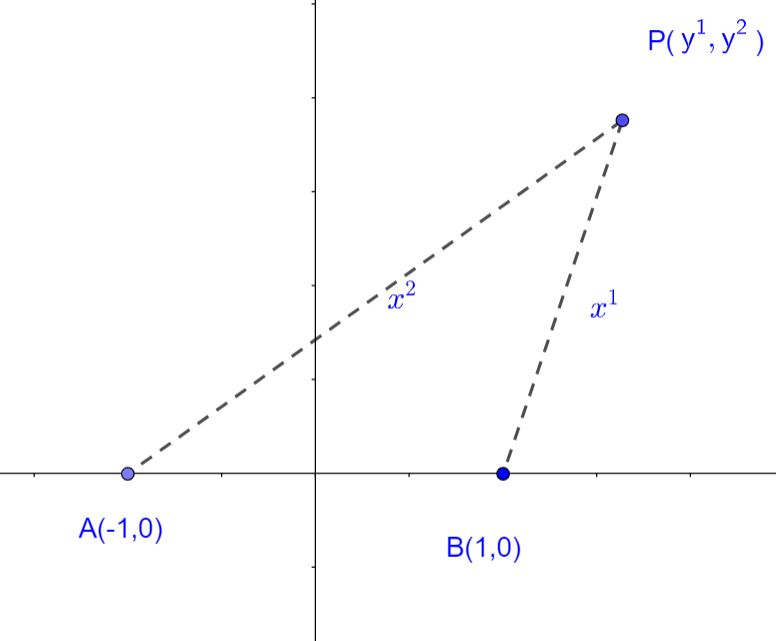
\includegraphics[scale=.4]{Bipolar.jpg}
\end{minipage}\hfill
\end{figure}
\begin{align}
\ (x^1)^2 &= \left( y^1-1\right) ^2 + \left(y^2\right)^2\\
\ (x^2)^2 &= \left( y^1+1\right) ^2 + \left(y^2\right)^2\\
\partial_1 (1) \quad\Rightarrow \quad x^1 &= \left( y^1-1\right)\partial_1 y^1  + \left(y^2\right)\partial_1 y^2\\
\partial_2 (2) \quad\Rightarrow \quad\ x^2 &= \left( y^1+1\right)\partial_2 y^1  + \left(y^2\right)\partial_2 y^2\\
\partial_2 (1) \quad\Rightarrow \quad 0 &= \left( y^1-1\right)\partial_2 y^1  + \left(y^2\right)\partial_2 y^2\\
\partial_1 (2) \quad\Rightarrow \quad\ 0 &= \left( y^1+1\right)\partial_1 y^1  + \left(y^2\right)\partial_1 y^2\\
\Rightarrow \quad & \left\{\begin{array}{ll}
\text{(3)-(6):}& \partial_1 y^1 = -\frac{x^1}{2}\\\\
\text{(4)-(5):}& \partial_2 y^1 = \frac{x^2}{2}\\\\
\text{(6):}& \partial_1 y^2 = \frac{y^1+1}{2y^2}x^1\\\\
\text{(5):}& \partial_2 y^2 = -\frac{y^1-1}{2y^2}x^2\\
\end{array}\right.\\
\text{Hence,}\quad J &= \left(\pdv{y^m}{x^n} \right) = \begin{pmatrix}
-\frac{x^1}{2} &\frac{x^2}{2}  \\
\frac{y^1+1}{2y^2}x^1 & -\frac{y^1-1}{2y^2}x^2 \\
\end{pmatrix}
\end{align}
\newpage
Be $A$ the metric tensor in Cartesian coordinate system. Then, going to a arbitrary coordinate system gives a metric tensor according to  
\begin{align}
\ & A^, = J^TAJ =J^TJ \quad \text{as}\quad A = \begin{pmatrix}
1 &0 \\
0& 1 \\
\end{pmatrix}\\
\Rightarrow\quad & A^, = \begin{pmatrix}
-\frac{x^1}{2} & \frac{y^1+1}{2y^2}x^1 \\
\frac{x^2}{2} & -\frac{y^1-1}{2y^2}x^2 \\
\end{pmatrix}\begin{pmatrix}
-\frac{x^1}{2} &\frac{x^2}{2}  \\
\frac{y^1+1}{2y^2}x^1 & -\frac{y^1-1}{2y^2}x^2 \\
\end{pmatrix}\\
\Rightarrow\quad & A^, =\frac{x^1x^2}{4(y^2)^2} \begin{pmatrix}
\ & \\
x^1x^2 &-\left[(y^1)^2 +(y^2)^2-1)\right] \\\\
-\left[(y^1)^2 +(y^2)^2-1)\right]  &x^1x^2\\
\ & 
\end{pmatrix}
\end{align}
We use plane geometry to express expression (11) as  a function of only $(x^1,x^2)$. For the triangle $APB$ in the figure below, we have
\begin{figure}[h]
\centering
\begin{minipage}[t]{.5\textwidth}
%\centering
\vspace{0pt}
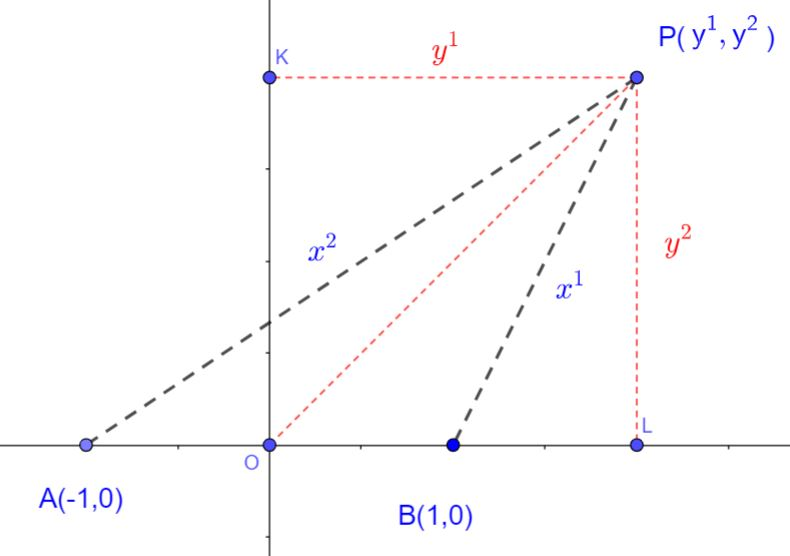
\includegraphics[scale=.4]{Bipolar2.jpg}
\end{minipage}\hfill
\end{figure}
\begin{align}
\ \left |  OP \right |^2 &= \frac{(x^1)^2+(x^2)^2}{2} - \underbrace{\frac{\left | AB \right|^2}{4}}_{=1}\\
\Rightarrow\quad (y^1)^2 +(y^2)^2 &= \frac{(x^1)^2+(x^2)^2}{2} - 1
\end{align}
The area $K$ of the triangle can be expressed in two ways
\begin{align}
\ K &= \half y^2\left | AB \right| = y^2\\
\text{and} \quad K &= \sqrt{s(s-x^1)(s-x^2)(s-2)}\\
\text{with}\quad s &= \half (x^1+x^2+2)\\
\text{hence}\quad (y^2)^2 &= \frac{1}{16}(x^1+x^2+2)(x^1+2)(x^2+2)(x^1+x^2)
\end{align}
So we get from (11):
\begin{align}
A^, =\frac{4x^1x^2}{(x^1+x^2+2)(x^1+2)(x^2+2)(x^1+x^2)} \begin{pmatrix}
\ & \\
x^1x^2 &2-\frac{(x^1)^2+(x^2)^2}{2} \\\\
2-\frac{(x^1)^2+(x^2)^2}{2}  &x^1x^2\\
\ & 
\end{pmatrix}
\end{align}
For the conjugate metric tensor we start from expression (11) and invert the metric tensor
\begin{align}
\left| A^,\right| &= \left[ \frac{x^1x^2}{4(y^2)^2}\right]^2\left[(x^1x^2)^2 -\left((y^1)^2 +(y^2)^2-1\right)^2\right]\\
\text{hence}\quad \left(a^{,mn}\right) &= \frac{1}{\left| A^,\right|}\frac{x^1x^2}{4(y^2)^2} \begin{pmatrix}
\ & \\
x^1x^2 &\left[(y^1)^2 +(y^2)^2-1\right] \\\\
\left[(y^1)^2 +(y^2)^2-1\right]  &x^1x^2\\
\ & 
\end{pmatrix}\\
\ &= \frac{4(y^2)^2\begin{pmatrix}
\ & \\
x^1x^2 &\left[(y^1)^2 +(y^2)^2-1\right] \\\\
\left[(y^1)^2 +(y^2)^2-1\right]  &x^1x^2\\
\ & 
\end{pmatrix}}{x^1x^2\left[(x^1x^2)^2 -\left((y^1)^2 +(y^2)^2-1\right)^2\right]} \\
\text{with} \quad x^1x^2&= \sqrt{\left[(y^1-1)^2 +(y^2)^2\right]\left[(y^1+1)^2 +(y^2)^2\right]}
\end{align}
$$\blacklozenge$$
\newpage

\section{p79-exercise 15}
\begin{tcolorbox}
Given $\Phi = a_{mn}dx^m dx^n$, with $a_{11} = a_{22}= 0$ but $a_{12} \ne 0$, show that $\Phi$ may be written in the form $$ \Phi = \epsilon\Psi^2_1- \epsilon\Psi^2_2 + \Phi_2$$ where $\Phi_2$ is a homogeneous quadratic form in $ dx^3, dx^4, \dots ,dx^N $, $\epsilon = \pm 1$ , and where 
$$\Psi_1 = \frac{1}{\sqrt(2 \epsilon a_{12})}\left[ a_{12}(dx^1+dx^2) + (a_{13}+a_{23})dx^3+ \dots +(a_{1N}+a_{2N})dx^N \right]$$
$$\Psi_2 = \frac{1}{\sqrt(2 \epsilon a_{12})}\left[ a_{12}(-dx^1+dx^2) + (a_{13}-a_{23})dx^3+ \dots +(a_{1N}-a_{2N})dx^N \right]$$
\end{tcolorbox}
Using local Cartesian coordinates we have:
Be 
\begin{align}
\Phi &= a_{mn}dx^mdx^n\\ 
\end{align}
and consider the following sequences of terms: 
\begin{align}
\Psi_1 =  b_{11}dx^1+b_{12}dx^2 + b_{13}dx^3+ \dots +b_{1N}dx^N \\
\Psi_2 =  b_{21}dx^1+b_{22}dx^2 + b_{23}dx^3+ \dots +b_{2N}dx^N 
\end{align}
The expressions (3) and (4) contain all the terms of $\Phi$ with $(dx^1)^2,(dx^2)^2$ and $dx^1dx^2$. So, $\Phi$ can be expressed as 
\begin{align}
\Phi =\Psi_1^2 -\Psi_2^2 + \Phi_2 
\end{align}
With $\Phi_2 $ being a homogeneous form containing only terms in $dx^i dx^j \quad i,j > 2$.\\
We can express $\Psi_1^2 - \Psi_2^2$ as
\begin{align}
\Psi_1^2 - \Psi_2^2 &= \left \{ \begin{array}{l}(b_{11}^2 - b_{21}^2)(dx^1)^2 +(b_{12}^2 - b_{22}^2)(dx^2)^2 +(b_{13}^2 - b_{23}^2)(dx^3 )^2 + \dots +(b_{1N}^2 - b_{2N}^2)(dx^N)^2 +\\
 2( b_{11} b_{12}-b_{21} b_{22})dx^1dx^2+2( b_{11} b_{13}-b_{21} b_{23})dx^1dx^3+\dots + 2( b_{11} b_{1N}-b_{21} b_{2N})dx^1dx^N+\\
 2( b_{12} b_{13}-b_{22} b_{23})dx^2dx^3+2( b_{12} b_{14}-b_{22} b_{24})dx^2dx^4+\dots + 2( b_{12} b_{1N}-b_{21} b_{2N})dx^2dx^N+\\
 + \dots 2( b_{1j} b_{1k}-b_{2j} b_{2k})dx^kdx^j+\dots\quad j>2, \ k\ne j
\end{array} \right.
\end{align}
Equating the terms in (1) and (6) and taking into account (=given) $a_{11}=a_{22}=0$ and $a_{12} \ne0$ 
\begin{align}
\ &\left \{ \begin{array}{l}
 b_{11}^2 - b_{21}^2 =0\\
 b_{12}^2 - b_{22}^2 =0\\
 2\left(b_{11}b_{12} - b_{21}b_{22} \right) = a_{12}+a_{21}
\end{array}\right.\\
\Rightarrow \quad \ &\left \{ \begin{array}{l}
 b_{11}^2 = b_{21}^2 \\
 b_{12}^2 = b_{22}^2 \\
 \left(b_{11}b_{12} - b_{21}b_{22} \right) =a_{12}
\end{array}\right.\\
\Rightarrow\quad b_{11} = \pm b_{21}  &\quad b_{22} =\pm b_{12}\\ 
\Rightarrow\quad  &\left \{ \begin{array}{l} 
 \pm b_{11}b_{22} \mp b_{11}b_{22}  =a_{12}\\ 
\text{or}\\
\pm b_{12}b_{21} \mp b_{12}b_{21}  =a_{12}
\end{array}\right.\\
\end{align}
As $a_{12} \ne0$, the signs in the above expressions must be the same. Hence,
\begin{align}
&\left \{ \begin{array}{c} 
 2b_{11}b_{22} =\pm a_{12}\\ 
2 b_{12}b_{21} =\pm a_{12} 
\end{array}\right.
\end{align}
(12) can be satisfied with an infinite combination of $b_{11},b_{12},b_{21}, b_{22}$. Choose,
\begin{align} 
\ b_{11} = \sqrt{\frac{\epsilon a_{12}}{2 }}\quad b_{22} = \sqrt{\frac{\epsilon a_{12}}{2 }}\quad & b_{12} = \sqrt{\frac{\epsilon a_{12}}{2 }}\quad b_{21} = - \sqrt{\frac{\epsilon a_{12}}{2 }}\\
\text{with} \quad  \epsilon &= \pm 1\quad\text{so that}\quad \epsilon a_{12} \geq 0
\end{align}
Put $\xi = \sqrt{\frac{\epsilon a_{12}}{2 }}$. Then, (3) and (4) can be expressed as 
\begin{align}
\Psi_1 =  \xi dx^1+\xi dx^2 + b_{13}dx^3+ \dots +b_{1N}dx^1dx^N \\
\Psi_2 =  -\xi dx^1+\xi dx^2 + b_{23}dx^3+ \dots +b_{2N}dx^1dx^N 
\end{align}
What are the $b_{.j}\quad (j>2)$? \\From (6), e.g. for $j=3$,  identifying the terms in $dx^1dx^3$ and $dx^2dx^3$ we see that
\begin{align}
&\left \{ \begin{array}{l} 
 \xi b_{13}+\xi b_{23} =a_{13}\\ 
\xi b_{13}-\xi b_{23} =a_{23}\\ 
\end{array}\right.\\
\Rightarrow \quad &\left \{ \begin{array}{l} 
 b_{13}=\frac{a_{13}+a_{23}}{2\xi}\\ 
 b_{23}=\frac{a_{13}-a_{23}}{2\xi}
\end{array}\right.\\
\text{or, in general} \quad &\left \{ \begin{array}{ll} 
 b_{1j}=\frac{a_{1j}+a_{2j}}{2\xi}\\
 \ &\ (j>2)\\ 
 b_{2j}=\frac{a_{1j}-a_{2j}}{2\xi}
\end{array}\right.
\end{align}
Bring $\frac{1}{\xi}$ out in $\Psi_1, \Psi_2$. This gives
\begin{align}
\Psi_1 &= \frac{1}{\xi}\left( \xi^2( dx^1+ dx^2) + \frac{a_{13}+a_{23}}{2}dx^3+ \dots +\frac{a_{1N}+a_{2N}}{2}dx^N \right) \\
\Psi_2 &= \frac{1}{\xi}\left( \xi^2(- dx^1+ dx^2) + \frac{a_{13}-a_{23}}{2}dx^3+ \dots +\frac{a_{1N}-a_{2N}}{2}dx^N \right) \\
\Rightarrow \quad &\left \{ \begin{array}{l} 
\Psi_1 = \frac{\sqrt{2}}{\sqrt{\epsilon a_{12}}}\left( \frac{\epsilon a_{12}}{2 } (dx^1+ dx^2) + \frac{a_{13}+a_{23}}{2}dx^3+ \dots +\frac{a_{1N}+a_{2N}}{2}dx^N \right) \\\\
\Psi_2 = \frac{\sqrt{2}}{\epsilon\sqrt{\epsilon a_{12}}}\left( \frac{\epsilon a_{12}}{2 } (-dx^1+ dx^2) + \frac{a_{13}-a_{23}}{2}dx^3+ \dots +\frac{a_{1N}-a_{2N}}{2}dx^N \right) \\
\end{array}\right.\\
\Leftrightarrow \quad &\left \{ \begin{array}{l} \\
\Psi_1 = \frac{1}{\sqrt{2 \epsilon a_{12}}}\left(\epsilon a_{12}(dx^1+ dx^2) + (a_{13}+a_{23})dx^3+ \dots +(a_{1N}+a_{2N})dx^N \right) \\\\
\Psi_2 = \frac{1}{\sqrt{2 \epsilon a_{12}}}\left( \epsilon a_{12}(- dx^1+ dx^2) + (a_{13}-a_{23})dx^3+ \dots +(a_{1N}-a_{2N})dx^N \right) \\
\end{array}\right.
\end{align}
What about the factor $\epsilon = \pm1$ in the terms $\epsilon a_{12}(dx^1+ dx^2)$ and $\epsilon a_{12}(-dx^1+ dx^2)$ ? Consider the alternate form
\begin{align}
\ &\left \{ \begin{array}{l} \\
\Psi^,_1 = \frac{1}{\sqrt{2 \epsilon a_{12}}}\left( a_{12}(dx^1+ dx^2) + (a_{13}+a_{23})dx^3+ \dots +(a_{1N}+a_{2N})dx^N \right) \\\\
\Psi^,_2 = \frac{1}{\sqrt{2 \epsilon a_{12}}}\left(  a_{12}(- dx^1+ dx^2) + (a_{13}-a_{23})dx^3+ \dots +(a_{1N}-a_{2N})dx^N \right) \\
\end{array}\right.
\end{align}
Let's have a look at the terms in $dx^idx^j$ in $\Psi_1^{,2}-\Psi^{,2}_2$\\
\begin{align}
\ x_{11}(dx^1)^2+ 2x_{12}dx^1dx^2+x_{22}(dx^2)^2&= \frac{1}{2 \epsilon a_{12}}\left(( a_{12})^2(dx^1 + dx^2)^2 - ( a_{12})^2(-dx^1 + dx^2)^2\right)  \\
&= \frac{\epsilon a_{12}}{2}\left((dx^1 +  dx^2)^2 - (- dx^1 + dx^2)^2\right)  \\
&= \frac{\epsilon a_{12}}{2}\left((dx^1)^2 + 2 dx^1dx^2+  (dx^2)^2 - (dx^1)^2 + 2 dx^1dx^2-  (dx^2)^2\right)  \\
&= 2 \epsilon a_{12}dx^1dx^2 \\
\ 2x_{13}dx^1dx^3&= \frac{1}{2 \epsilon a_{12}}(2 a_{12}(a_{13}+a_{23})dx^1dx^3 - 2a_{12}(a_{13}-a_{23})dx^1dx^3) \\
\ &= \frac{1}{2 \epsilon a_{12}}(4 a_{12}a_{23})dx^1dx^3 \\
 & =  2\epsilon a_{23}dx^1dx^3\\
 \ 2x_{23}dx^2dx^3&= \frac{1}{2 \epsilon a_{12}}(2 a_{12}(a_{13}+a_{23})dx^1dx^3 - 2 a_{12}(a_{13}-a_{23})dx^1dx^3) \\
\ &= \frac{1}{2 \epsilon a_{12}}(4 a_{12}a_{23})dx^1dx^3 \\
 & =  2\epsilon a_{23}dx^1dx^3\\
\ 2x_{34}dx^3dx^4&=  \frac{1}{2 \epsilon a_{12}}\left(\begin{array}{l} 2 (a_{13}+ a_{23})(a_{14}+ a_{24}\\ - 2 (a_{13}- a_{23})(a_{14}- a_{24}) \end{array} \right)dx^3dx^4 \\
\ &= \frac{2\epsilon}{ a_{12}}\left(a_{23}a_{14}+a_{13}a_{24}\right)
\end{align}
We rewrite now the metric form $\Phi$ as 
$$\Phi =\epsilon \Psi_1^{,2}- \epsilon \Psi^{,2}_2 + \Phi_2 $$
From (28), (31) and (34) we see that the terms in $dx^1, dx^2$ in $\Phi =\epsilon \Psi_1^{,2}- \epsilon \Psi^{,2}_2 + \Phi_2$ correspond to the expected  metric form and that the other terms in $dx^j, dx^k, \ j,k \neq 1,2$ can be corrected in the remaining term $\Phi_2$.
\newpage

\section{p80-exercise 16}
\begin{tcolorbox}
Find the null geodesics of a 4-space with line element
$$ds^2=\epsilon \gamma\left(dx^2 +dy^2+dz^2-dt^2\right)$$ where $\gamma$ is an arbitrary function of $x,\ y,\ z,\ t$.
\end{tcolorbox}
We have:
\begin{align}
\left(a_{mn}\right) = \gamma\begin{pmatrix}
 1&0  & 0 & 0 \\
 0&  1& 0 & 0 \\
 0&0  & 1 &  0\\
 0& 0 & 0 & -1 \\
\end{pmatrix} \quad \left(a^{mn}\right) = \frac{1}{\gamma}\begin{pmatrix}
 1&0  & 0 & 0 \\
 0&  1& 0 & 0 \\
 0&0  & 1 &  0\\
 0& 0 & 0 & -1 \\
\end{pmatrix}\\
\end{align}
Be $(x^1,x^2,x^3,x4) \equiv (x,y,z,t)$.\\
The general conditions for a null geodesic are
\begin{align}
\left \{ \begin {array}{l}
\dv[2]{x^r}{v} + \Gamma^r_{mn}\dv{x^m}{v}\dv{x^n}{v} = 0\\\\
\ a_{mn}dx^mdx^n =0
\end{array}\right.
\end{align}
When calculating $[mn,r] = \half\left(\partial_n a_{mr}+\partial_m a_{nr}-\partial_r a_{mn} \right) $ we note that $\left(a_{mn}\right)$ is a diagonal matrix, ans so is also $\left(a^{mn}\right)$. Hence $\Gamma^r_{mn}$ will contain only one term:
\begin{align}
\ & \Gamma^r_{mn} = a^{RR}[mn,R]\\
\Rightarrow \quad & \left \{ \begin{array}{llll}
\ i)& m,n \neq R \ \wedge \ m \neq n&:& [mn,R]=0\\\\
\ ii)& m \neq n = R \ \vee \  n \neq m = R&:& [mn,R]=\half \partial_m a_{RR}\\\\
\ iii)& m =n \neq R &:& [mn,R]=-\half \partial_R a_{mn}\\\\
\ iv)& m =n= R &:& [mn,R]=\half \partial_R a_{RR}\\\\
\end{array}\right.
\end{align}\\
and for the $\Gamma^r_{mn}$:\\
\begin{align}
\Rightarrow \quad & \left \{ \begin{array}{llll}
\ i)& m,n \neq R \ \wedge \ m \neq n &:& \Gamma^R_{mn}=0\\\\
\ ii)& m \neq n = R \ \vee \  n \neq m = R &:& \Gamma^R_{nR}=\frac{1}{2 \gamma} \partial_n \gamma \\\\
\ iii)& m =n \neq R = \ 1,2,3 &:& \Gamma^R_{kk}=-\frac{1}{2 \gamma}  \partial_R \gamma\\
\ & m =n \neq R =4 &:& \Gamma^4_{kk}=\frac{1}{2 \gamma}  \partial_R \gamma\\\\
\ iv)& m =n= R &:& \Gamma^R_{RR}=\frac{1}{2 \gamma}  \partial_R \gamma\\\\
\end{array}\right.
\end{align}
Let's compute 
\begin{align}
\ A_r \equiv \dv[2]{x^r}{v} + \Gamma^r_{mn}\dv{x^m}{v}\dv{x^n}{v}
\end{align}
and take $v = x^4$, so $x^1, \  x^2,  \ x^3 = f(x^4)$. (In the following $d_kx^j \equiv \dv{x^j}{{(x^{k})}}\ , \ d^2_kx^j \equiv \dv[2]{x^j}{{(x^{k})}}$)
\begin{align}
\left \{ \begin{array}{ll}
\ A_1 = &  d^2_4x^1+ \Gamma^1_{mn}d_4x^md_4x^n\\
\ A_2 = &  d^2_4x^2+ \Gamma^2_{mn}d_4x^md_4x^n\\
\ A_3 = &  d^2_4x^3+ \Gamma^3_{mn}d_4x^md_4x^n\\
\ A_4 = &   \Gamma^4_{mn}d_4x^md_4x^n
\end{array} \right.
\end{align}
and get from (8) and (6):
\begin{align}
\ A_1 -d^2_4x^1 &= \left \{ \begin{array}{l}\frac{1}{\gamma}  \partial_2 \gamma \ d_4x^1d_4x^2  + \frac{1}{\gamma}  \partial_3 \gamma \ d_4x^1 d_4x^3+\frac{1}{\gamma}  \partial_4 \gamma \ d_4x^1 d_4x^4\\\\
\ + \underbrace{\frac{1}{2\gamma}\partial_1 \gamma (d_4x^1)^2}_{= \left \{ \begin{array}{l} \frac{1}{\gamma} \partial_1 \gamma (d_4x^1) (d_4x^1)\\
\  - \frac{1}{2\gamma} \partial_1 \gamma (d_4x^1)^2 \end{array} \right.} - \frac{1}{2\gamma}\partial_1 \gamma (d_4x^2)^2- \frac{1}{2\gamma}\partial_1 \gamma (d_4x^3)^2+ \frac{1}{2\gamma}\partial_1 \gamma (d_4x^4)^2
 \end{array} \right.\\
 &= \left \{ \begin{array}{l}\frac{1}{\gamma} \partial_1 \gamma d_4x^1 d_4x^1 + \frac{1}{\gamma}  \partial_2 \gamma \ d_4x^1d_4x^2  + \frac{1}{\gamma}  \partial_3 \gamma \ d_4x^1 d_4x^3+\frac{1}{\gamma}  \partial_4 \gamma \ d_4x^1 d_4x^4\\\\
\ - \frac{1}{2\gamma}\partial_1 \gamma (d_4x^1)^2 - \frac{1}{2\gamma}\partial_1 \gamma (d_4x^2)^2- \frac{1}{2\gamma}\partial_1 \gamma (d_4x^3)^2+ \frac{1}{2\gamma}\partial_1 \gamma (d_4x^4)^2
 \end{array} \right.\\\\
  &= \left \{ \begin{array}{l}\frac{1}{\gamma}d_4x^1 \left(\partial_1 \gamma  d_4x^1  + \partial_2 \gamma \ d_4x^2  + \partial_3 \gamma \  d_4x^3+ \partial_4 \gamma \ d_4x^4 \right)\\\\
\ - \frac{1}{2\gamma}\partial_1 \gamma \left(\underbrace{(d_4x^1)^2 +(d_4x^2)^2+(d_4x^3)^2- (d_4x^4)^2}_{= a_{mn}dx^m dx^n = 0 }\right)
 \end{array} \right.\\
 \Rightarrow \quad A_1 &= d^2_4x^1+ \frac{1}{\gamma}d_4x^1 < \grad \gamma|\partial_4 \overline{x} >
\end{align}
with $\grad \gamma =  (\partial_x \gamma,\ \partial_y \gamma, \ \partial_z \gamma, \ \partial_t \gamma)$ and $ \partial_4 \overline{x} =  (\partial_t x, \ \partial_t y , \ \partial_t z, \ \partial_t t)$.\\
So for the geodesic with get for the first coordinate $$d^2_4x^1+ \frac{1}{\gamma}d_4x^1 < \grad \gamma|\partial_4 \overline{x} > = 0 $$
Doing analogous calculations give the following set of equations
\begin{align}
\ d^2_4x^k+ \frac{1}{\gamma}d_4x^k < \grad \gamma|\partial_4 \overline{x} > = 0 
\end{align}
Note that for $k=4$ we have as $\ d_4x^4 = 1$ and $\ d^2_4x^4 = 0$:
\begin{align}
 \frac{1}{\gamma}< \grad \gamma|\partial_4 \overline{x} > = 0 \\
 \Rightarrow \quad < \grad \gamma|\partial_4 \overline{x} > = 0 
\end{align}
Note that this means that $\grad \gamma$ and $\partial_4 \overline{x}$ are orthogonal 4-vectors.\\
So the set of equations in (14) reduce to the following set of $2^{nd}$ order differential equations:
\begin{align}
\ & \left  \{ \begin{array}{l}
\ x^{,,} = 0\\
\ y^{,,} = 0\\
\ z^{,,} = 0\\
\ t = t\\
\end{array} \right.
\Rightarrow  \left  \{ \begin{array}{l}
\ x = x_1t+x_0\\
\ y =y_1t+y_0\\
\ z = z_1t+z_0\\
\ t = t\\
\end{array} \right.
\end{align}
This is the equations of 4-space cone, which was expected as the metric is localy a Minkowksi-like metric. 
$$\blacklozenge$$
\newpage

\section{p80-exercise 17}
\begin{tcolorbox}
In a space $V_N$ the metric tensor is $a_{mn}$. Show that the null geodesics are unchanged if the metric tensor is changed to $b_{mn} = \gamma a_{mn} $, $\gamma$ being a function of the coordinates.
\end{tcolorbox}
Null geodesics are determined by the following set of equations
\begin{align}
\ & \left \{  \begin {array}{l}
\dv[2]{x^r}{v} + \Gamma^r_{mn}\dv{x^m}{v}\dv{x^n}{v} = 0\\\\
\ a_{mn}dx^mdx^n =0
\end{array}\right.\\
\text{We have}\quad  \Gamma^r_{mn} & = a^{rs}[mn,s]\\
\ & = \frac{1}{\gamma}a^{rs}\gamma[mn,s]\\
\text{We have also }\quad  b^{rs} & = \frac{1}{\gamma}a^{rs}\\
\text{Indeed }\quad  a^{rs}a_{rs}&= \delta^r_t\\
\Rightarrow\quad  \frac{1}{\gamma}a^{rs}\gamma a_{rs}&= \delta^r_t\\
\Rightarrow\quad  \frac{1}{\gamma}a^{rs}b_{rs}&= \delta^r_t\\
\Rightarrow\quad  \frac{1}{\gamma}a^{rs} &= b_{rs}\\
\text{So (3) becomes}\quad  \Gamma^r_{mn} & =b^{rs}\gamma[mn,s]
\end{align}
Be $ [mn,s]^{'} $ the Christoffel symbol associated with the metric $b_{mn}= \gamma a_{mn}$. Then with  $$[mn,s]^, = \half \left(\partial_n \gamma a_{ms}+\partial_m \gamma a_{ns}-\partial_s \gamma a_{mn} \right)$$ we get
\begin{align}
\ [mn,s]^{'} &= \gamma [mn,s] + \half\left( a_{ms}\partial_n \gamma+a_{ns}\partial_m \gamma-a_{mn}\partial_s \gamma \right)
\end{align}
Substitute $\gamma [mn,s]$ from (10) in (9) we get
\begin{align}
\Gamma^r_{mn} & =\underbrace{b^{rs}\gamma[mn,s]^,}_{=\Gamma^{'r}_{mn}}  - \underbrace{\half b^{rs}\left( a_{ms}\partial_n \gamma+a_{ns}\partial_m \gamma-a_{mn}\partial_s \gamma \right)}_{\coloneqq Q}\\
\text{with}\quad Q &= \half b^{rs}\left( a_{ms}\partial_n \gamma+a_{ns}\partial_m \gamma-a_{mn}\partial_s \gamma \right)\\
&= \half \gamma \left( \underbrace{a^{rs}a_{ms}}_{ = \delta^r_m}\partial_n \gamma+\underbrace{a^{rs}a_{ns}}_{ = \delta^r_n}\partial_m \gamma-a^{rs}a_{mn}\partial_s \gamma \right)\\
\ Q \times \dv{x^m}{v}\dv{x^n}{v} &= \half \gamma \left( \underbrace{\delta^r_m\dv{x^m}{v}}_{=\dv{x^r}{v}} \underbrace{\partial_n \gamma \dv{x^n}{v}}_{= \dv{\gamma}{v}}+\underbrace{\delta^r_n\dv{x^n}{v}}_{=\dv{x^r}{v}}\underbrace{\partial_m \gamma\dv{x^m}{v}}_{= \dv{\gamma}{v}}-a^{rs}\partial_s \gamma \underbrace{a_{mn}\dv{x^m}{v}\dv{x^n}{v}}_{ = 0 \ \text{by(1)}} \right)\\
&= \half \gamma \left( \dv{x^r}{v}\dv{\gamma}{v} +\dv{x^r}{v}\dv{\gamma}{v} \right)\\
&= \left(\gamma\dv{\gamma}{v} \right)  \dv{x^r}{v}
\end{align}
So from (11) and (16), (1) can be expressed as 
\begin{align}
\dv[2]{x^r}{v} + \Gamma^{'r}_{mn}\dv{x^m}{v}\dv{x^n}{v} = \left(\gamma\dv{\gamma}{v} \right)  \dv{x^r}{v}
\end{align}
By (2.449) page 46 we see that the vector 
$\dv[2]{x^r}{v} + \Gamma^{'r}_{mn}\dv{x^m}{v}\dv{x^n}{v}$ is collinear to $\dv{x^r}{v}$. Also $b_{mn}\dv{x^m}{v}\dv{x^n}{v} = 0$. And hence (17) determines the geodesic null lines. So both expressions (1) and (17) are equivalent to determine the same geodesic null lines in the space $V_N$ equipped with the metric $a_{mn}$ or  $b_{mn}$
$$\blacklozenge$$
\newpage


\section{p80-exercise 18}
\begin{tcolorbox}
Are the relations $$T_{|rs} =T_{|sr} $$ $$T_{r|sk} =T_{r|ks} $$ true (a) in curvilinear coordinates in Euclidean space, (b) in a general Riemannian space?
\end{tcolorbox}
$$\boldsymbol{T_{|rs} \questeq  T_{|sr}}$$
We have $T|_r = \partial_rT$ (see (2.528) page 53) \\
\begin{equation}
  \begin{split}
  \ & \boldsymbol{T_{|rs}}\\\\
   \ & T|_{rs} = \partial^2_{rs}T - \Gamma^m_{rs}T|_m
  \end{split}
\quad\leftrightarrow\quad
  \begin{split}
 \ & \boldsymbol{T_{|sr}}\\\\
   \ & T|_{sr} = \partial^2_{sr}T - \Gamma^m_{sr}T|_m
  \end{split}
\end{equation}
As $\partial^2_{rs} =\partial^2_{sr}$ and $\Gamma^m_{rs} =\Gamma^m_{sr}$ we can conclude that $\boldsymbol{T_{|rs} =T_{|sr}}$ in both cases (a) and (b).\\\\
$$\boldsymbol{\diamond}$$\\\\
$$\boldsymbol{T_{r|sk} \questeq  T_{r|ks}}$$
\begin{equation}
  \begin{split}
  \ & \boldsymbol{T_{r|sk}}\\\\
  \ & A_{rs} \coloneqq T_{r|s} = \partial_{s}T_r - \Gamma^m_{rs}T_m\\
  \ & A_{rs|k}= \partial_k A_{rs} - \Gamma^m_{rk}A_{ms} -  \Gamma^m_{sk}A_{rm}\\
  \ & A_{ms}=  \partial_{s}T_m - \Gamma^n_{ms}T_n\\
  \ & A_{rm} = \partial_{m}T_r - \Gamma^n_{rm}T_n\\
  \ & A_{rs|k}= \left \{\begin{array}{l}
   \underbrace{\partial^2_{sk}T_r}_{*} - T_m\partial_{k}\Gamma^m_{rs} - \underbrace{\Gamma^m_{rs}\partial_{k}T_m}_{**} \\\\
   \ -\underbrace{\Gamma^m_{rk}\partial_{s}T_m}_{***} +\Gamma^m_{rk} \Gamma^n_{ms}T_n \\\\
   \ - \underbrace{\Gamma^m_{sk}\partial_{m}T_r}_{****} +\underbrace{\Gamma^m_{sk} \Gamma^n_{rm}T_n}_{*****}
  \end{array}\right.
  \end{split}
\quad\leftrightarrow\quad
  \begin{split}
 \ & \boldsymbol{T_{r|sk}}\\\\
  \ & B_{rk} \coloneqq T_{r|k} = \partial_{k}T_r - \Gamma^m_{rk}T_m\\
  \ & B_{rk|s}= \partial_s B_{rk} - \Gamma^m_{rs}B_{mk} -  \Gamma^m_{ks}B_{rm}\\
  \ & B_{mk}=  \partial_{k}T_m - \Gamma^n_{mk}T_n\\
  \ & B_{rm}=  \partial_{m}T_r - \Gamma^n_{rm}T_n\\
  \ & B_{rk|s}= \left \{\begin{array}{l}
  \underbrace{\partial^2_{ks}T_r}_{*} - T_m\partial_{s}\Gamma^m_{rk} - \underbrace{\Gamma^m_{rk}\partial_{s}T_m}_{***} \\\\
   \ -\underbrace{\Gamma^m_{rs}\partial_{k}T_m}_{**} +\Gamma^m_{rs} \Gamma^n_{mk}T_n \\\\
   \ - \underbrace{\Gamma^m_{ks}\partial_{m}T_r}_{****} +\underbrace{\Gamma^m_{ks} \Gamma^n_{rm}T_n}_{*****}
  \end{array}\right.
  \end{split}
\end{equation}\begin{align}
\Rightarrow\quad A_{rs|k} - B_{rk|s} &= T_m\left( \underbrace{\partial_{s}\Gamma^m_{rk}-\partial_{k}\Gamma^m_{rs}+\Gamma^n_{rk} \Gamma^m_{ns}- \Gamma^n_{rs} \Gamma^m_{nk} }_{\coloneqq R^s{.rmn}}\right) 
\end{align}
So, $T_{r|sk} =  T_{r|ks}$ only if $T_m R^s_{.rmn} = 0$ and as $T_m$ is an arbitrary tensor, $R^s_{.rmn}$ must vanish for $T_{r|sk} =  T_{r|ks}$.\\\\
$\textbf{Note:}$\\
Although $\Gamma^n_{rk}$ is not a tensor, the quantity $R^s_{.rmn}$ is. Indeed, as both $A_{rs|k} - B_{rk|s}$ and $ T_m$ have the tensor character, this implies that $R^s_{.rmn}$ is a tensor.
Now, for an Euclidean space equipped with Cartesian coordinates all $\Gamma^n_{rk} $ are constant and vanish. So, $R^s_{.rmn}$ = 0. Let's consider a change of coordinate system from Cartesian to curvilinear coordinate system. Then, by the tensor character of $R^{'a}_{\ .bcd}$ we have,
\begin{align}
\ R^{'a}_{\ .bcd} = R^s_{.rmn}\partial_s x^{'a} \partial_{('b)} x^{r} \partial_{('c)} x^{m} \partial_{('d)} x^{n}
\end{align}
but $R^s_{.rmn} =0$ in the Cartesian coordinate system and so is $R^{'a}_{\ .bcd}$\\
$\textbf{Conclusion:}$\\
In a general Riemannian space $T_{r|sk} \neq  T_{r|ks}$ but $T_{r|sk} =  T_{r|ks}$ in a curvilinear Euclidean space.
$$\blacklozenge$$
\newpage

\section{p80-exercise 19}
\begin{tcolorbox}
Consider a $V_N$ with indefinite metric form. For all points $P$ lying on the cone of  geodesic null lines drawn from  $O$, the definition 2.611 for Riemannian coordinates apparently breaks down. Revise the definition of Riemannian coordinates so as to include such points.
\end{tcolorbox}
For geodesic null lines we have (2.445 page 46)
\begin{align}
\left \{ \begin{array}{l}
\dv[2]{x^r}{u} + \Gamma^r_{mn}\dv{x^m}{u}\dv{x^n}{u} = 0\\
\ a_{mn}\dv{x^m}{u}\dv{x^n}{u} = 0
\end{array}\right.
\end{align}
or (2.448 page 46)
\begin{align}
\left \{ \begin{array}{l}
\dv[2]{x^r}{v} + \Gamma^r_{mn}\dv{x^m}{v}\dv{x^n}{v} = \lambda(v) \dv{x^r}{v}\\
\ a_{mn}\dv{x^m}{v}\dv{x^n}{v} = 0
\end{array}\right.
\end{align}
where by suitable choice of the parameter $v$ , $\lambda(v) $ can be made any preassigned function of $v$.
\begin{align}
\text{(2)} \RAr \dv[2]{x^r}{v} &=   \lambda \dv{x^r}{v}-\Gamma^r_{mn}\dv{x^m}{v}\dv{x^n}{v} \\
\RAr \dv[3]{x^r}{v} &=   \dv{\lambda }{v}\dv{x^r}{v}+ \lambda \dv[2]{x^r}{v}+ A^r_{.mns}\dv{x^m}{v}\dv{x^n}{v}\dv{x^s}{v} \\
\text{with}\RAr A^r_{.mns} &= - \partial_s \Gamma^r_{mn} + 2 \Gamma^r_{sp}\Gamma^p_{mn}
\end{align}
Expanding $x^r$ in a Taylor series around a point $O(a^r)$ we get (for ease of notation we put $p^r \coloneqq \dv{x^r}{v}$)
\begin{align}
\ x^r &= a^r + v p^r + \half v^2\lambda  p^r -  \half v^2\Gamma^r_{mn}p^mp^n+\frac{1}{6}v^3\dv{\lambda  }{v}p^r + \frac{1}{6}v^3\lambda  \dv{p^r}{v} + \frac{1}{6}v^3A^r_{.mns}p^mp^np^s+\dots\\
&= a^r + \left(v  + \half v^2\lambda  +\frac{1}{6}v^3\dv{\lambda  }{v}\right)p^r -  \half v^2\Gamma^r_{mn}p^mp^n + \frac{1}{6}v^3\lambda  \dv{p^r}{v} + \frac{1}{6}v^3A^r_{.mns}p^mp^np^s+\dots
\end{align}
Put $x^{'r} \coloneqq   v\xi(v) p^r$ with $\xi(v) = \left(1  + \half v\lambda  +\frac{1}{6}v^2\dv{\lambda  }{v}\right)$. Hence (7) becomes
\begin{align}
\ x^r &= a^r + x^{'r} -  \frac{1}{2\xi ^2}\Gamma^r_{mn}x^{'m}x^{'n} + \frac{1}{6}v^3\lambda  \left( \frac{p^{'r}}{v\xi} - \frac{\xi + v\xi^{'}}{v^2\xi^2}x^{'r}\right) + \frac{1}{6\xi ^3}A^r_{.mns}x^{'m}x^{'n}x^{'s}+\dots\\
\ & = a^r + \tau(v) x^{'r}+ \frac{v^2\lambda  }{6\xi}p^{'r} -  \frac{1}{2\xi ^2}\Gamma^r_{mn}x^{'m}x^{'n}   + \frac{1}{6\xi ^3}A^r_{.mns}x^{'m}x^{'n}x^{'s}+\dots\\
\text{with}\spatie & \tau(v)  \coloneqq 1-\frac{v\lambda  }{6\xi^2}\left( \xi + v\xi^{,}\right)
\end{align}\\
Is the Jacobian non-zero?
\begin{align}
\pdv{x^r}{x^{'q}}  & = \tau(v)\delta^r_q+ \frac{v^2\lambda  }{6\xi}\dv{\delta^r_q}{v} -  \frac{1}{\xi ^2}\Gamma^r_{mq}x^{'m}   + \frac{1}{2\xi ^3}A^r_{.mnq}x^{'m}x^{'n}+\dots
\end{align}
In the infinitesimal neighbourhood of $O$ we have \\
\begin{align}\left \{ \begin{array}{l} 
v \rightarrow 0\\  
\xi \rightarrow 1\\
\xi^{'} \rightarrow \frac{\lambda }{2}\\ 
x^{'m} \rightarrow 0\\
\tau \rightarrow 1 
\end{array} \right.\\
\end{align}
so that the Jacobian determinant becomes
\begin{align}
\left| \pdv{x^r}{x^{'q}} \right| &= \left| \tau\delta^r_q \right| =\tau ^N = 1
\end{align}
$\textbf{Conclusion:}$\\
So in order to define a Riemannian coordinates system which is still valid on the null geodesics, it is sufficient to define the Riemannian coordinates around $O$ as $$ x^{'r} \coloneqq   v\xi(v) p^r$$ with $$\xi(v) = \left(1  + \half v\lambda +\frac{1}{6}v^2\dv{\lambda }{v}\right) $$
and $\lambda $, by suitable choice of $v$, being any pre-defined function of $v$.
$$\blacklozenge$$
\newpage

\chapter{Curvature of space}
\pagebreak[4]

\section{p82 - Exercise}
\begin{tcolorbox}
Explain why the surfaces of an ordinary cylinder and an ordinary cone are to be regarded as "flat" in the sense of our definition.
\end{tcolorbox}
The reason is because those surfaces can be "unwrapped" like the figure below shows. 
\begin{figure}[h]
%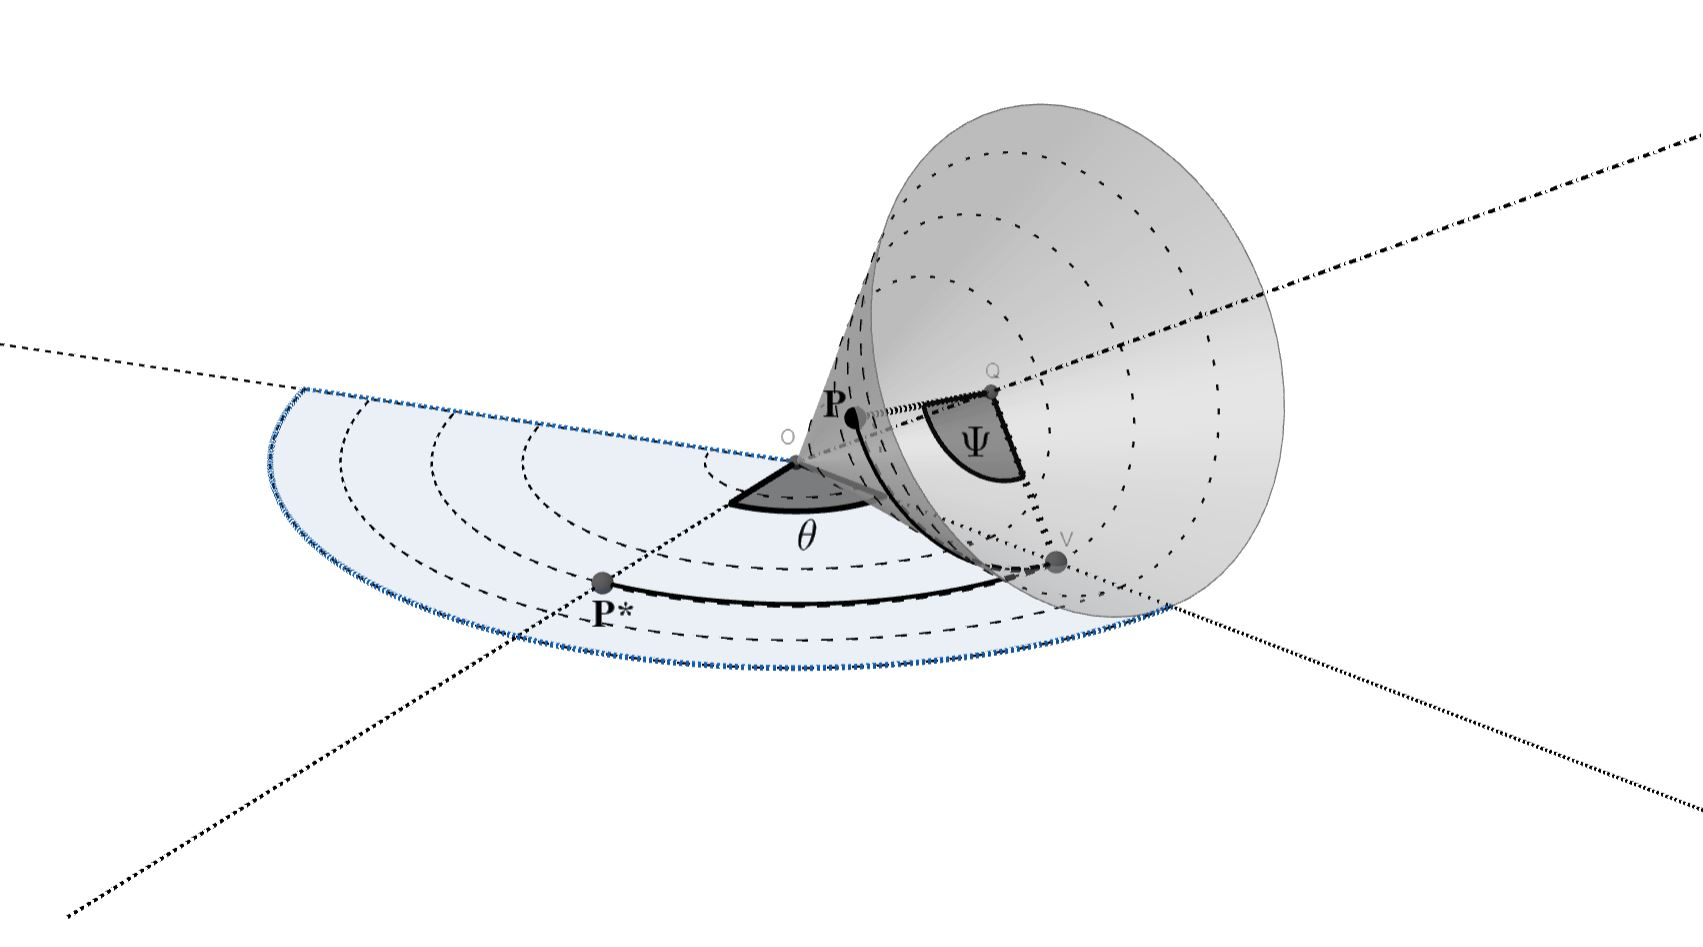
\includegraphics[scale=.5]{Conemapping.jpg}
%\tdplotsetmaincoords{0}{10};
\pgfplotsset{every axis/.append style={
		view={-30}{-30*1},
		%view={-90}{-30*0},
		scale=1.5,
		axis lines=center,
		axis on top,
		%xlabel={$y$},
		%ylabel={$x$},
		%zlabel={$z$},
               axis x line=middle,    % put the x axis in the middle
               axis y line=middle,    % put the y axis in the middle
                axis z line=middle,    % put the z axis in the middle
               %axis line style={-stealth}, % arrows on the axis
               axis line style={draw=none}
            }}
            


            
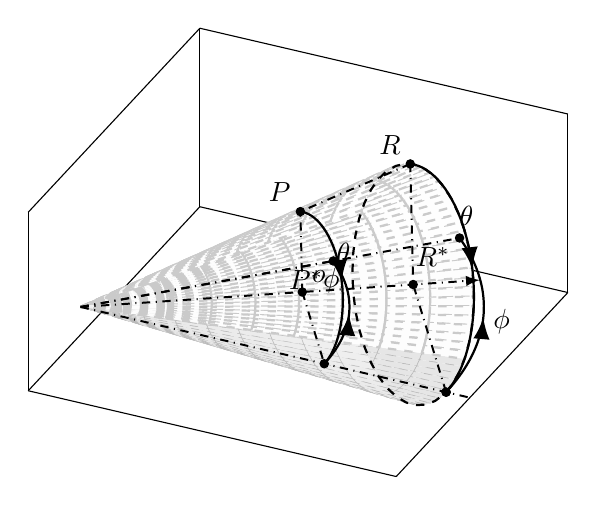
\begin{tikzpicture}[angle/.style={black,thick}]
\tikzmath{\r=1.5;\h=5;\q=asin((\r/\h)); \p=-\q*1 ; \k= \r/\h;};
\q, \h,\p, \k;
    \pgfplotsset{ticks=none};
    \pgfplotsset{compat=1.12};
\begin{axis}
		[
		axis equal=true,
		zmin=-\h*0,
		zmax=\r*1.2,
		]
		%draw the cylinder whiwh is tilted so that it 'rolls' on the x-y plane and oriented along the y-axis
		\addplot3 [surf,dashed,very thin,	mesh/interior colormap=
		{bw}{color=(gray!10) color=(gray!5)},
		colormap= {bw}{color=(black!10) color=(white!10)},
		domain=115:115+180,
		y domain=0:\h,
		samples=40,
		samples y=10,
		z buffer=sort,]
		({\y*cos(\p)+1*\y*tan(\q)*sin(x)*sin(\p)},{1*y*tan(\q)*cos(x)},{-\y*sin(\p)+1*\y*tan(\q)*sin(x)*cos(\p)});
		
		
		%draw the cylinder whiwh is tilted so that it 'rolls' on the x-y plane and oriented along the y-axis
		\addplot3 [surf,	dashed,thick,	mesh/interior colormap=
		{bw}{color=(gray!1) color=(gray!5)},
		colormap= {bw}{color=(black!1) color=(white!1)},
		domain=-65:115,
		y domain=0:\h,
		samples=40,
		samples y=10,
		z buffer=sort,]
		({\y*cos(\p)+1*\y*tan(\q)*sin(x)*sin(\p)},{1*y*tan(\q)*cos(x)},{-\y*sin(\p)+1*\y*tan(\q)*sin(x)*cos(\p)});
	
		%add a base circle to emphasize the cone shape
		\addplot3 [black,thick,dashed,samples=40,	samples y=0,	domain=0.0:360,]({\h*cos(\p)+1*\h*tan(\q)*sin(x)*sin(\p)},{1*\h*tan(\q)*cos(x)},{-\h*sin(\p)+1*\h*tan(\q)*sin(x)*cos(\p)});
		% add an arcsegment on the base
		\addplot3 [decoration={markings, mark = at position 0.5 with {\arrow[scale = 1.5]{latex}}},postaction ={decorate},black,thick,samples=40,	samples y=0,	domain=60:-90,]({\h*cos(\p)+1*\h*tan(\q)*sin(x)*sin(\p)},{1*\h*tan(\q)*cos(x)},{-\h*sin(\p)+1*\h*tan(\q)*sin(x)*cos(\p)});%node[midway,right] {$\Psi$};;
		% add an arcsegment at 2/3 pf the cone
		\addplot3 [decoration={markings, mark = at position 0.5 with {\arrow[scale = 1.5]{latex}}},postaction ={decorate},black,thick,samples=40,	samples y=0,	domain=60.0:-90,]({2*\h/3*cos(\p)+2*\h/3*tan(\q)*sin(x)*sin(\p)},{2*\h/3*tan(\q)*cos(x)},{-2*\h/3*sin(\p)+2*\h/3*tan(\q)*sin(x)*cos(\p)});%node[midway,right] {$x^1$};
		
		
		% labels of arcsegments on the cone
		 \coordinate (F) at ({2*\h/3*cos(\p)+2*\h/3*tan(\q)*sin(20)*sin(\p)},{2*\h/3*tan(\q)*cos(20)},{-2*\h/3*sin(\p)+2*\h/3*tan(\q)*sin(20)*cos(\p)});
 		\draw[](F) node[{anchor=north west}] {$\theta$};
 		\coordinate (F2) at ({\h*cos(\p)+\h*tan(\q)*sin(20)*sin(\p)},{\h*tan(\q)*cos(20)},{-\h*sin(\p)+\h*tan(\q)*sin(20)*cos(\p)});
 		\draw[](F2) node[{anchor=north west}] {$\theta$};
 		
		%relevant points
		\coordinate (O) at ({ 0},{0},{0});%origin
		\coordinate (P) at ({ \h*1},{\h*0},{0});%point  P on the cone 
		\coordinate (C) at ({1.2* \h*cos(\p)},{\h*0},{1.2*\h*sin(-\p)});
		\coordinate (A) at ({1.* \h*cos(\p)},{\h*0},{1.*\h*sin(-\p)});
		\coordinate (Q) at ({1.* \h/cos(\p)},{\h*0},{0.*\h*sin(-\p)});

		%\node[tdplot_main_coords,{anchor=south west},red] at (P){$o$};
		%\draw[dashed,line width = 0.25mm] (O) --(P) ;%node[midway,right] {$x^1$};
		\draw[dashdotted,- latex,line width = 0.25mm] (O) --(C) ;%node[midway,right] {$x^1$};
		%\draw[dashdotted,line width = 0.25mm] (Q) --(A) ;%node[midway,right] {$x^1$};
		%draw points on cone
		\coordinate (W) at ({ \h/cos(\p)},{\h*0},{0.*\h*sin(-\p)});
		\coordinate (N) at ({1.2 *\h},{\h*0},{0.*\h*sin(-\p)});
		\coordinate (R) at ({2/3* \h/cos(\p)},{\h*0},{0.*\h*sin(-\p)});
		\coordinate (S) at ({2*\h/3*cos(\p)+2*\h/3*tan(\q)*sin(60)*sin(\p)},{2*\h/3*tan(\q)*cos(60)},{-2*\h/3*sin(\p)+2*\h/3*tan(\q)*sin(60)*cos(\p)});
		\coordinate (T) at ({2*\h/3*cos(\p)+0*\h/3*tan(\q)*sin(60)*sin(\p)},{0},{-2*\h/3*sin(\p)+0*\h/3*tan(\q)*sin(60)*cos(\p)});
		\draw[fill=black](A) circle(1.5pt);%node[{anchor=north west}] {$A$};
		\draw[fill=black](Q) circle(1.5pt);%node[{anchor=north west}]{$A$};;
		\coordinate (Y) at ({\h*cos(\p)+\h*tan(\q)*sin(60)*sin(\p)},{\h*tan(\q)*cos(60)},{-\h*sin(\p)+\h*tan(\q)*sin(60)*cos(\p)});
		\draw[fill=black](Y) circle(1.5pt)node[{anchor=south east}] {$R$};
		\draw[fill=black](W) circle(1.5pt);%node[{anchor=north west}] {$O$};;
		\draw[fill=black](R) circle(1.5pt);%node[{anchor=north west}]{$V$};;
		\draw[fill=black](S) circle(1.5pt)node[{anchor=south east}] {$P$};
		\draw[fill=black](T) circle(1.5pt)node[{anchor=south west}] {$o$};
		\draw[dashdotted,- latex,line width = 0.25mm] (O) --(N) ;%node[midway,right] {$x^1$};
		\draw[dashdotted,line width = 0.25mm] (T) --(R) ;%node[midway,right] {$x^1$};
		\draw[dashdotted,line width = 0.25mm] (T) --(S) ;%node[midway,right] {$x^1$};
		
		\draw[dashdotted,line width = 0.25mm] (Y) --(A) ;%node[midway,right] {$x^1$};
		\draw[dashdotted,line width = 0.25mm] (Y) --(S) ;%node[midway,right] {$x^1$};
		\draw[dashdotted,line width = 0.25mm] (W) --(A) ;%node[midway,right] {$x^1$};


		
		%projection onthe xy-plane
		%arcsegments of points P and R
		\begin{scope}
		\addplot3 [decoration={markings, mark = at position 0.5 with {\arrow[scale = 1.5]{latex}}},postaction ={decorate},samples=40,black,thick,samples=40,	samples y=0,	domain=0:150,]
			({2/3*\h/cos(\q)*cos(x*sin(\q))},{2/3*\h/cos(\q)*sin(x*sin(\q))},{0});%node[midway,right] {$theta$};
		\addplot3 [decoration={markings, mark = at position 0.5 with {\arrow[scale = 1.5]{latex}}},postaction ={decorate},samples=40,black,thick,samples=40,	samples y=0,domain=0:150,]
			({\h/cos(\q)*cos(x*sin(\q))},{\h/cos(\q)*sin(x*sin(\q))},{0});%node[midway,right] {$x^1$};
		\end{scope}
		%projections  R*, P* of points R,P
		\coordinate (U) at ({2/3*\h/cos(\q)*cos(150*sin(\q))},{2/3*\h/cos(\q)*sin(150*sin(\q))},{0});
		\coordinate (V) at ({\h/cos(\q)*cos(150*sin(\q))},{\h/cos(\q)*sin(150*sin(\q))},{0});
		

		\draw[dashdotted,line width = 0.25mm] (O) --(U) ;%node[midway,right] {$x^1$};
		\draw[dashdotted,line width = 0.25mm] (O) --(V) ;%node[midway,right] {$x^1$};
		
		%dots and labels of P* and R*
 		
 		\draw[fill=black](U) circle(1.5pt)node[{anchor=north east}] {$P^{*}$};
		\draw[fill=black](V) circle(1.5pt)node[{anchor=north east}] {$R^{*}$};
 		%add labels of angles at a right place
 		 \coordinate (G) at({2/3*\h/cos(\q)*cos(90*sin(\q))},{2/3*\h/cos(\q)*sin(90*sin(\q))},{0});
 		\draw[](G) node[{anchor=south east}] {$\phi$};
 		 \coordinate (M)  at({\h/cos(\q)*cos(90*sin(\q))},{\h/cos(\q)*sin(90*sin(\q))},{0});
 		\draw[](M) node[{anchor=north west}] {$\phi$};
\end{axis}
\end{tikzpicture}\\
\caption{Unwrapping of a cone}
\end{figure}\\
For the cone, we can for each point $\ P $ on the cone, lying on a distance $\ h $ from the apex and making an angle $\Psi $,  associate on a plane,  a  point $ P^* $ lying at the same  distance $ h $ from the apex, taken as origin for the coordinate system, and making an angle $\theta =  k\Psi $ with $ k $ a constant depending on the shape of the cone. This pair of coordinates are polar coordinates with $ r \in (-\infty, + \infty)$ and $\theta \in [0, 2k\pi)$. 
The same reasoning can be applied to a cylinder which is a cone with the apex at $\infty$. In that case the coordinate system becomes a Cartesian coordinate system. \\
As a continuous mapping exist from polar to orthogonal Cartesian coordinates both  coordinate system can be written under the required form (3.101) and so can be called "flat".

$$\blacklozenge$$
\newpage

\section{p83 - Exercise}
\begin{tcolorbox}
What are the values of $R^s_{.rmn}$ in an Euclidean plane, the coordinates being rectangular Cartesians? Deduce the values of the components of this tensor for polar coordinates from its tensor character, or else by direct calculation.
\end{tcolorbox}
See 2.64 page 139 (exercise 18).
$$\blacklozenge$$
\newpage

\section{p86 - Exercise}
\begin{tcolorbox}
Show that in a $V_2$ all the components of the covariant curvature tensor either vanish or are expressible in terms of $R_{1212}$.
\end{tcolorbox}
We have (3.115) and (3.116)
\begin{align}
\left \{ \begin{array}{l}
\ R_{rsmn} =  - R_{srmn}\\
\ R_{rsmn} =  - R_{rsnm}\\
\ R_{rsmn} =   R_{mnrs}\\
\ R_{rsmn} + R_{rmns}+R_{rnsm}=0
\end{array} \right.
\end{align}
It is clear from the two first identities that  in pairs $(rs)$ and $(mn)$ both indices have to be different when the tensor is not $0$. So we only have to consider $R_{1212}$,  $R_{1221}$, $R_{2112}$ and $R_{2121}$.\\
The two first  identities gives us:
\begin{align}
 R_{1221}= -R_{1212}\\
 R_{2112}= -R_{1212}\\
 R_{2121}= -R_{2112} = R_{1212}
\end{align}
The third identity does give us any additional information.
The fourth identity gives us only trivial statements:
\begin{align}
 R_{1212} + \underbrace{R_{1122}}_{=0}+\underbrace{R_{1221}}_{=- R_{1212} } = 0\\
 \underbrace{R_{1221}}_{=- R_{1212}} + R_{1212}+\underbrace{R_{1122}}_{=0 } = 0\\
 \underbrace{R_{2112}}_{=- R_{1212}} + \underbrace{R_{2121}}_{=R_{1212}}+\underbrace{R_{2211}}_{=0} = 0\\
 \underbrace{R_{2121}}_{= R_{1212}} + \underbrace{R_{2211}}_{=0}+\underbrace{R_{2112}}_{= -R_{1212}} = 0
\end{align}
$\textbf{Conclusion:}$\\
We get the identities (2), (3) and (4) in function of $R_{1212}$ and all vanish if $R_{1212} = 0$
$$\blacklozenge$$
\newpage

\section{p86-87 - clarification}
\begin{tcolorbox}
\textit{The number of independent components of the covariant curvature tensor in a space of N dimensions is} $$\frac{1}{12}N^2\left(N^2-1\right)$$
\end{tcolorbox}
We have (3.115) and (3.116)
\begin{align}
\left \{ \begin{array}{l}
R_{rsmn} =  - R_{srmn}\\
R_{rsmn} =  - R_{rsnm}\\
R_{rsmn} =   R_{mnrs}\\
R_{rsmn} + R_{rmns}+R_{rnsm}=0
\end{array}\right.
\end{align}
It is clear from the two first identities that  in the tuple $(rs)$ and $(mn)$ both indices have to be different when the component is not $0$. So we only have to consider the component with the pair of tuples $(r,s)$ and $m,n)$ with $r \neq s$ and $m \neq n$.
For the tuple $(r,s)$ we have $N$ possibilities to draw an index for $r$ but for $s$ only $N-1$ indices remain as $r \neq s$. So for the tuple $(r,s)$ we get $N(N-1)$ possibilities. But note by the first identity $R_{rsmn} =  - R_{srmn}$ that we only have to consider the half of this quantity as once we have chosen a tuple $(r,s)$ we also know  the component for the tuple $(s,r)$. So the total number of possibilities we have for  $(r,s)$ is $M = \half N(N-1)$. The same yields for the tuple $(mn)$. So, we get in total $M^2$ possibilities according to the two first identities.\\
The third identity $R_{rsmn} =   R_{mnrs}$ puts an extra constraint on the number of possibilities as we have to subtract from $M^2$ the number of possibilities covered by this third identity. Note that, once we have chosen a tuple $(rs)$ we have to exclude the tuple $(m,n) =  (r,s)$ as the identity $R_{rsrs} =   R_{rsrs}$ becomes trivial.. So for the first tuple we have $M$ possibilities, but once chosen, only $M-1$ remain for the second tuple. So we get $M(M-1)$ possibilities. But, again we only have to take half of these possibilities as the identities $R_{rsmn} =   R_{mnrs}$ and $ R_{mnrs} = R_{rsmn}$ are equivalent.\\
So the total number of possibilities reduces to $$ M^2 - \half M(M-1) \quad \text{with} \quad M=\half N(N-1) $$
What about the fourth identity $$R_{rsmn} + R_{rmns}+R_{rnsm}=0$$
First we note that this identity implies that all indices are different as it becomes trivial in the other cases. This is a consequence of the first 3 identities. Indeed, we know already that
\begin{align}
\left \{ \begin{array}{l}
\ r \neq s\\
\ m \neq n\\
\ (r,s) \neq (m,n)\\
\end{array} \right.
\end{align}
Let's consider the following cases
\begin{align}
\left \{ \begin{array}{llll}
\ r = m&\rightarrow m\neq s \  m\neq n \ r\neq n&\rightarrow & R_{rsrn} + \underbrace{R_{rrns}}_{=0}+\underbrace{R_{rnsr}}_{= -R_{rnrs}= -R_{rsrn}}=0\\
\ r = n&\rightarrow n\neq s \  m\neq n \ r\neq s&\rightarrow & R_{rsmr} + \underbrace{R_{rmrs}}_{= -R_{mrrs}= -R_{rsmr}}+\underbrace{R_{rrsm}}_{=0}=0\\
\ s = m&\rightarrow m\neq r \  n\neq s \ r\neq s&\rightarrow & R_{rssn} + \underbrace{R_{rsns}}_{= -R_{rssn}}+\underbrace{R_{rnss}}_{=0}=0\\
\ s = n&\rightarrow r\neq s \  m\neq s \ m\neq n&\rightarrow & R_{rsms} + \underbrace{R_{rmss}}_{=0}+\underbrace{R_{rssm}}_{= -R_{rsms}}=0
\end{array} \right.
\end{align}
So indeed, once two indices are equal, the fourth identity becomes trivial and does not put extra constraints to the number of possibilities. For the tuple $(r,s,m,n)$ we have $N$ possibilities to draw an index for $r$, for $s$ only $N-1$, for $m$ only $N-2$ and for $n$ only $N-3$ indices remain as $r \neq s\neq m\neq n$. The maximum number of constraint generated by the fourth identity is thus $$N(N-1)(N-2)(N-3)$$
But here again double counts occur. Indeed the fourth identity is true for the $6$ tuples $$(rsmn),(rmsn) ,(rmns),(rsnm),(rnsm),(rnms)$$ as first entry    in the identity. The same reasoning is valid for the tuples $(n...), \ (s...) \ (m...) $. \\So in total we get $6\times4 = 24$ equivalent identities and the number of constraints generated by the fourth identity reduces to  $$\frac{1}{24}N(N-1)(N-2)(N-3)$$
Note that this number of constraints vanish for $N \leq 3$.\\
Putting it all together the number of independent components of $R_{rsmn}$ becomes
\begin{align}
\mho &= M^2 - \half M(M-1)-\frac{1}{24}N(N-1)(N-2)(N-3)\\
&= \half M(M+1)-\frac{1}{24}N(N-1)(N-2)(N-3)\\
&= \frac{1}{8} N(N-1) \left(N(N-1)+2\right)-\frac{1}{24}N(N-1)(N-2)(N-3)\\
&= \frac{N}{24} \left( 3N^2-6N^2+9N-6-N^3+3N^2+3N^2-9N-2N+6 \right)\\
&= \frac{1}{12}N^2 \left( N^2-1\right)
\end{align}
$$\blacklozenge$$
\newpage


\section{p82 - Exercise}
\begin{tcolorbox}
Would the study of geodesic deviation enable us to distinguish between a plane and a right circular cylinder?
\end{tcolorbox}
For geodesic lines we have
\begin{align}
\dv[2]{x^r}{u} + \Gamma^r_{mn}\dv{x^m}{u}\dv{x^n}{u} = 0\\
\end{align}
with the fundamental tensor for a cylindar (see exercise page 27)
\begin{align} 
(a_{mn}) = \begin{pmatrix}
 1& 0 \\
0 & r^2 \\
\end{pmatrix}
\end{align}
As no element of this tensor is a function of the coordinates, it is clear that all Christoffel symbols vanish and the geodesic curve are solutions of the simple system of $2^{nd}$ order differential equations
\begin{align}
\dv[2]{x^r}{u}  = 0
\end{align}
Hence
\begin{align}
x^r  &= \kappa u + \mu\\
\text{or}\quad x^r &= \kappa^r u
\end{align}
by choosing the origin of the coordinates system with the initial condition position of the point.
Choosing polar coordinates $\phi, z$ as coordinates, the distance one walks when following a geodesic is given by
\begin{align}
 s= \int_{u_0}^{u_1}\sqrt{(r^2(d\phi)^2 + (dz)^2)}
\end{align}
and if we take $u=\phi$ as independent a parameter, by (6) we get 
\begin{align}
 s-s_0 &= \int_{\psi_0}^{\psi_1}\sqrt{(r^2 + \kappa^2)}d\psi \equiv g(\psi - \psi_0)\\
 \text{or}\quad s&= \int_{\psi_0}^{\psi_1}\sqrt{(r^2 + \kappa^2)}d\psi \equiv g\psi
\end{align}
by introducing transformed coordinates $s^{'}= s-s_0$ and $\psi^{'} =\psi - \psi_0$.\\
and thus we get 
\begin{align}
 z = m s^{'}
\end{align}
\begin{figure}[H]
%\centering
\begin{minipage}[t]{.4\textwidth}
%\centering
\vspace{0pt}
%\includegraphics[scale=.5]{p85_ex1.png}
\tdplotsetmaincoords{0}{10};
\pgfplotsset{every axis/.append style={
		view={-10*1}{-30*1},
		%view={-90}{-30*0},
		scale=3,
		%axis lines=center,
		axis on top,
		xlabel={$y$},
		ylabel={$x$},
		zlabel={$z$},
               axis x line=middle,    % put the x axis in the middle
               axis y line=middle,    % put the y axis in the middle
                axis z line=middle,    % put the z axis in the middle
               axis line style={-stealth}, % arrows on the axis
            }}
\begin{tikzpicture}

  \def\r{0.5};
    \def\H{10};
    \pgfplotsset{ticks=none};
    \pgfplotsset{compat=1.12};

    	
	\begin{axis}
		[
		xmin=-1.5,
		xmax=1.5,
		ymin=-1.5,
		ymax=1.5,
		zmin=0.0,
		zmax=10.0,
		]
		%draw the cylinder
		\addplot3 [surf,	dashed,thick,domain=0:10,	mesh/interior colormap=
		{bw}{color=(gray!10) color=(gray!50)},
		colormap= {bw}{color=(white!10) color=(white!10)},
		y domain=0:1*pi,samples=10,
		samples y=40,z buffer=sort,]
		({\r*cos(deg(y))},{\r*sin(deg(y))},{x});
						%draw the curves
				%base cylinder
		
		\addplot3 +[no markers,dotted,thick, black,samples=51,	samples y=0,	domain=-pi/2+0.16666667:pi/2+0.16666667,variable=\t]
		({0.5*sin(deg(\t))},{0.5*cos(deg(\t))},{0 });
		\addplot3 +[no markers,dotted,gray,thick, black,samples=51,	samples y=0,	domain=0:2*pi,variable=\t]
		({0.5*sin(deg(\t))},{0.5*cos(deg(\t))},{10 });		
		\addplot3 +[no markers,dotted,gray,thick, black,samples=51,	samples y=0,	domain=-pi/2+0.16666667:pi/2+0.16666667,variable=\t]
		({0.5*sin(deg(\t))},{0.5*cos(deg(\t))},{5 });	
		
		
				%curve1
		\addplot3 [ultra thick, black,samples=51,	samples y=0,	domain=0:pi/2+0.16666667,variable=\t]
		({0.5*sin(deg(\t))},{0.5*cos(deg(\t))},{\t });
		
		\addplot3 [thick, dashed,thick,black,samples=51,	samples y=0,	domain=pi/2+0.16666667:3*pi/2+0.17776667,variable=\t]
		({0.5*sin(deg(\t))},{0.5*cos(deg(\t))},{\t });
		
			\addplot3 [ultra thick, black,samples=51,	samples y=0,	domain=3*pi/2+0.17776667:2*pi,variable=\t]	
		({0.5*sin(deg(\t))},{0.5*cos(deg(\t))},{\t });
		

		
		%curve2
			\addplot3 [ultra thick, black,samples=51,	samples y=0,	domain=0:pi/2+0.16666667,variable=\t]
		({0.5*sin(deg(\t))},{0.5*cos(deg(\t))},{\t*1.5 });
		
		\addplot3 [dashed,thick,black, samples=51,	samples y=0,	domain=pi/2+0.16666667:3*pi/2+0.17776667,variable=\t]	
		({0.5*sin(deg(\t))},{0.5*cos(deg(\t))},{\t*1.5});
		
		\addplot3 [ultra thick, black,samples=51,	samples y=0,	domain=3*pi/2+0.17776667:2*pi,variable=\t]	
		({0.5*sin(deg(\t))},{0.5*cos(deg(\t))},{\t*1.5 });
		
		%2D graph
	    	\coordinate (P) at (0.7,0,6);
		\coordinate (O) at (0.7,0,3);
		\coordinate (Q) at (0.7+0.6,0,6);
		\coordinate (R) at (0.7+0.6,0,3);
		\coordinate (xO) atat (0.7+0.05,0,3+0.2);
		\coordinate (xY) at (0.7+0.05,0,3+2.5);
		\coordinate (xZ) at (0.7+10*0.05,0,3+0.2);
		
		%labeling points
		\node[tdplot_main_coords,{anchor=south west}] at (xY){$z$};
		\node[tdplot_main_coords,{anchor=south west}] at (xZ){$s$};
		
		%drawing the lines
		%region
		\draw (O)--(P);
		\draw (Q)--(P);
		\draw (Q)--(R);
		\draw (R)--(O);
		%axes
		\draw[-stealth,thick] (xO)--(xY);
		\draw [-stealth,thick](xO)--(xZ);
		%curves
		\coordinate (p1) at (0.75+10*0.05,0,3+1.5);
		\coordinate (p2)  at (0.7+10*0.05,0,3+1.1);
		\draw (xO)--(p1);
		\draw(xO)--(p2);
		%point on cylinder
		\coordinate (q1) at ({0.5*sin(360},{0.5*cos(360)},{9.4});
		\coordinate (r1) at ({0.5*sin(360},{0.5*cos(360)},{6.3});
		\draw[] (q1) circle (5pt);
		\draw[] (r1) circle (5pt);

		%point in graph
		\coordinate (q2) at ({1.12},{0},{4.4});
		\coordinate (r2) at ({1.12},{0},{4.0});
		%arrows
		  \draw[dotted, -stealth,thick, postaction={decorate}] (q1) .. controls (0.5, 0,10) .. (q2) ;
		  \draw[dotted, -stealth, thick, postaction={decorate}] (r1) .. controls (0.5, 0,7) .. (r2) ;
		  %initial conditions
		  %vectors points
		 \coordinate (icO) at ({0},{0.5},{0});
		\coordinate (iC1) at ({0.5*1.1},{0.5},{1.1});
		\coordinate (iC2) at ({0.5},{0.5},{1.5});
		%arrows
		  \draw[ -stealth,gray, very thick,postaction={decorate}] (icO) -- (iC1) ;
		  \draw[ -stealth, ,gray, very thick,postaction={decorate}] (icO) --(iC2) ;
		  %angles
		  
		  
	% draw arc using the three points and a radius
	  % arcs
  	%\tdplotdefinepoints (0,0.,0)(0.5*1.1,0.5,1.1)(0.5,0.5,1.5);
  	  	%\tdplotdefinepoints (0,0.,0)  (0,1,1.1)(0.5,0.5,1.5);
  	  	%\tdplotdefinepoints (0.55,0.5,1.1)(0.5,0.5,1.5)(0,0.5,0);
  	%\tdplotdrawpolytopearc[<->]{3}{anchor=north west}{$\theta$}
  	
  	%arrows
		  \draw[ stealth-stealth,thick, postaction={decorate}] (iC1) .. controls (0.45, 0,0.5) .. (iC2) node[midway,right] {$\theta$};;
		  %\draw[dotted, -stealth, thick, postaction={decorate}] (p2) .. controls (0.5, 0,0.5) .. (r2) ;
		  
		  \draw[ stealth-stealth,thick, postaction={decorate}] (p1) .. controls (1.25, 0,4.2) .. (p2) node[midway,right] {$\theta$};;
		  
\end{axis}

\end{tikzpicture}\\
\end{minipage}\hfill
\caption{Geodesics on a cylinder}
\end{figure}
The above figure illustrates what an observer sees when walking along geodesics on the cylinder.  He only can measure the distance $s^{'}$ and the displacement along $z$ and by (10) can only draw a chart like the one seen on the right of the cylinder. A "flatlander" would see the same chart when walking along geodesics in his plane.\\\\
\textbf{Conclusion:} No, studying the geodesic deviation on a right circular cylinder does not enable us to say on which surface we are.
$$\blacklozenge$$
\newpage

\section{p93 - Exercise}
\begin{tcolorbox}
For rectangular cartesians in Euclidean 3-space, show that the general solution of 3.311 is $\eta^r = A^r s+B^r $, where $A^, \ B^r$ are constants. verify this by elementary geometry. 
\end{tcolorbox}
We have equation 3.111
\begin{align}
\fdv[2]{\eta^r}{s}+ R^r_{.smn} p^s \eta^m p^n=0
\end{align}
From exercise on page 83 we know that $R^r_{.smn}=0$ in an Euclidean space. Also, in such spaces, the Christoffels symbols vanish and equation (1) reduces to $ \dv[2]{\eta}{s} = 0$. And so, $$\eta^r = A^r s+B^r $$

This is also easily deducted from a geometrical point of view. In an Euclidean space, the geodesics are straight lines. For an infinitesimal change in the geodesic family parameter $v$, we can assume that a vector, going perpendicular from 1 point from one geodesic with parameter $v$  to another infinitesimal close  geodesic with parameter $v+dv$,  will also be perpendicular on this geodesic. This situation is depicted in figure (a). We conclude that $\overrightarrow{AA^{'}} \ \parallel \ \overrightarrow{PP^{'}}$. This can also be deducted from Thales theorem (see fig. (b)). 
\begin{figure}[H]%
    \centering
    \subfloat[]{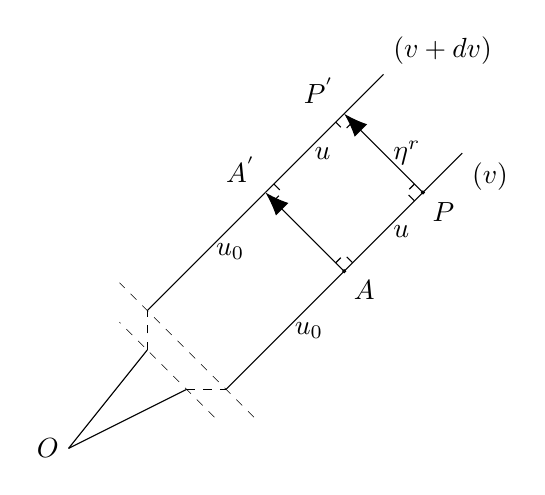
\begin{tikzpicture}[scale=0.5]
\tikzset{
    right angle quadrant/.code={
        \pgfmathsetmacro\quadranta{{1,1,-1,-1}[#1-1]}     % Arrays for selecting quadrant
        \pgfmathsetmacro\quadrantb{{1,-1,-1,1}[#1-1]}},
    right angle quadrant=1, % Make sure it is set, even if not called explicitly
    right angle length/.code={\def\rightanglelength{#1}},   % Length of symbol
    right angle length=2ex, % Make sure it is set...
    right angle symbol/.style n args={3}{
        insert path={
            let \p0 = ($(#1)!(#3)!(#2)$) in     % Intersection
                let \p1 = ($(\p0)!\quadranta*\rightanglelength!(#3)$), % Point on base line
                \p2 = ($(\p0)!\quadrantb*\rightanglelength!(#2)$) in % Point on perpendicular line
                let \p3 = ($(\p1)+(\p2)-(\p0)$) in  % Corner point of symbol
            (\p1) -- (\p3) -- (\p2)
        }
    }
}
\tikzstyle{point}=[circle,thick,draw=black,fill=black,inner sep=0pt,minimum width=4pt,minimum height=4pt]

\coordinate [label=left:$O$](O) at (0,-0.5);
\coordinate (p1) at (2.,2);
\coordinate (q1) at (3,1);
\coordinate (p2) at (2,3);
\coordinate (q2) at (4,1);
\coordinate  [label=above left:$A^{'}$](p3) at (5,6);
\coordinate [label=below right:$A^{}$](q3) at (7,4);
\coordinate [label=above left:$P^{'}$](p4) at (8-1,9-1);
\coordinate [label=below right:$P^{}$](q4) at (10-1,7-1);
\coordinate [label=above right:$(v+dv)$](p5) at (8,9);
\coordinate [label=below right:$(v)$](q5) at (10,7);
%draw lines
\draw[thin] (O) -- (p1);
\draw[thin] (O) --  (q1);
\draw[dashed] (p1) -- (p2);
\draw[dashed] (q1) -- (q2);

\draw[] (p3) -- (p2)node[midway,below,right] {$u_0$};;
\draw[] (q3) -- (q2)node[midway,below,right] {$u_0$};;

\draw[] (p3) -- (p4)node[midway,above,right] {$u$};
\draw[] (q3) -- (q4)node[midway,below,right] {$u$};

\draw[] (p5) --(p4);
\draw[] (q5) --(q4);

\draw[very thin,dashed] ($(q2)!-1cm!(p2)$) -- ($(p2)!-1cm!(q2)$);
\draw[very thin,dashed] ($(q1)!-1cm!(p1)$) -- ($(p1)!-1cm!(q1)$);


\draw (q3)  circle[radius=1pt];
\draw (q4)  circle[radius=1pt];
\draw[-{Latex[length=3mm]}] (q3)--(p3) ;%node[right]{with fixed length};
\draw[-{Latex[length=3mm]}] (q4)--(p4) node[midway, , right]{$\eta^r$};


\draw [dashed,right angle symbol={q3}{p3}{q4}];
\draw [dashed,right angle symbol={q4}{p4}{q3}];
\draw [dashed,right angle symbol={p3}{q3}{p4}];
\draw [dashed,right angle symbol={p4}{p3}{q4}];
%labeling points

\end{tikzpicture}}
	\qquad
    \subfloat[]{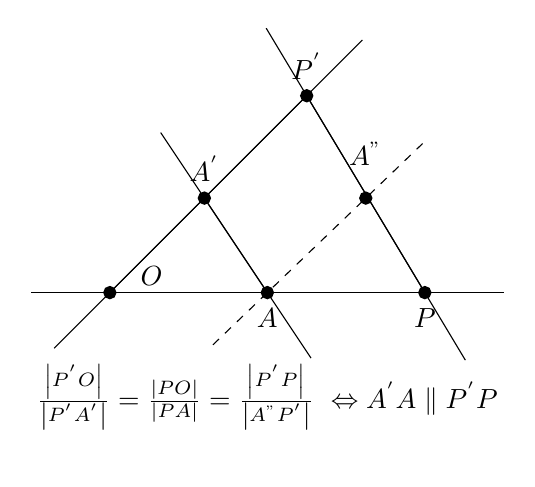
\begin{tikzpicture}
\tikzstyle{point}=[circle,thick,draw=black,fill=black,inner sep=0pt,minimum width=4pt,minimum height=4pt]
    \node (P)[point,label={[label distance=-1cm]210:$O$}] at (0,0) {};
    \node (B)[point,label={[label distance=0cm]-90:$A$}] at (2.0,0) {};
    \node (Q)[point,label={[label distance=0cm]-90:$P$}] at (4,0) {};
    \node (C)[point,label={[label distance=0cm]90:$A^{'}$}] at (1.5*0.8,1.5*0.8) {};
    \node (R)[point,label={[label distance=0cm]90:$P^{'}$}] at (2.5,2.5) {};
    \node (Bb)[point,label={[label distance=0.21cm]90:$A^{"}$}] at (3.25,1.5*0.8) {};

    \node (A)[label={[label distance=0cm]:$\frac{\left|P^{'}O\right|}{\left|P^{'}A^{'}\right|}=\frac{\left|PO\right|}{\left|PA\right|} =\frac{\left|P^{'}P\right|}{\left|A^{"}P^{'}\right|}\ \Leftrightarrow A^{'}A \parallel P^{'}P  $}] at(2,-2) {};

    \draw[] (P) edge node  {} (B);
    \draw[] (B) edge node  {} (Q);
    \draw[] (P) edge node  {} (C);
    \draw[] (C) edge node  {} (R);
    %\draw[] (C) edge node  {} (Bb);

    \draw[] (B) edge node  {} (C);
    %\draw[] (C) edge node  {} (A);

    \draw[] (Q) edge node  {} (R);

    \draw[] ($(P)!-1cm!(Q)$) -- ($(Q)!-1cm!(P)$);
    \draw[] ($(P)!-1cm!(R)$) -- ($(R)!-1cm!(P)$);
    \draw[] ($(C)!-1cm!(B)$) -- ($(B)!-1cm!(C)$);
    \draw[] ($(R)!-1cm!(Q)$) -- ($(Q)!-1cm!(R)$);
    \draw[dashed] ($(Bb)!-1cm!(B)$) -- ($(B)!-1cm!(Bb)$);
\end{tikzpicture} }
\caption{Geometrical deduction of the geodesical deviation equation in an Euclidean space.}
\end{figure}
Hence, we than can say that,
$$ \frac{\left|AA^{'}\right|}{u_0}=\frac{\left|PP^{'}\right|}{u}  $$
or, $$ \eta^r = A^r u + B^r $$ as the reference point $A$ can be chosen arbitrarily on the line $AP$.
$$\blacklozenge$$
\newpage

\begin{comment}
\section{p83 - clarification}
\begin{tcolorbox}
$V_2$ from family of geodesics
\end{tcolorbox}
\begin{figure}[h]%
    \centering
    \subfloat[]{{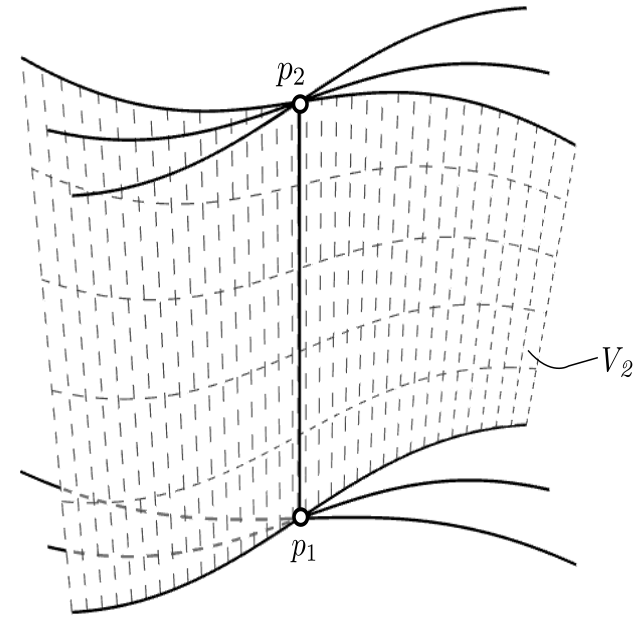
\includegraphics[width=6cm]{p87_a} }}%
    \qquad
    \subfloat[]{{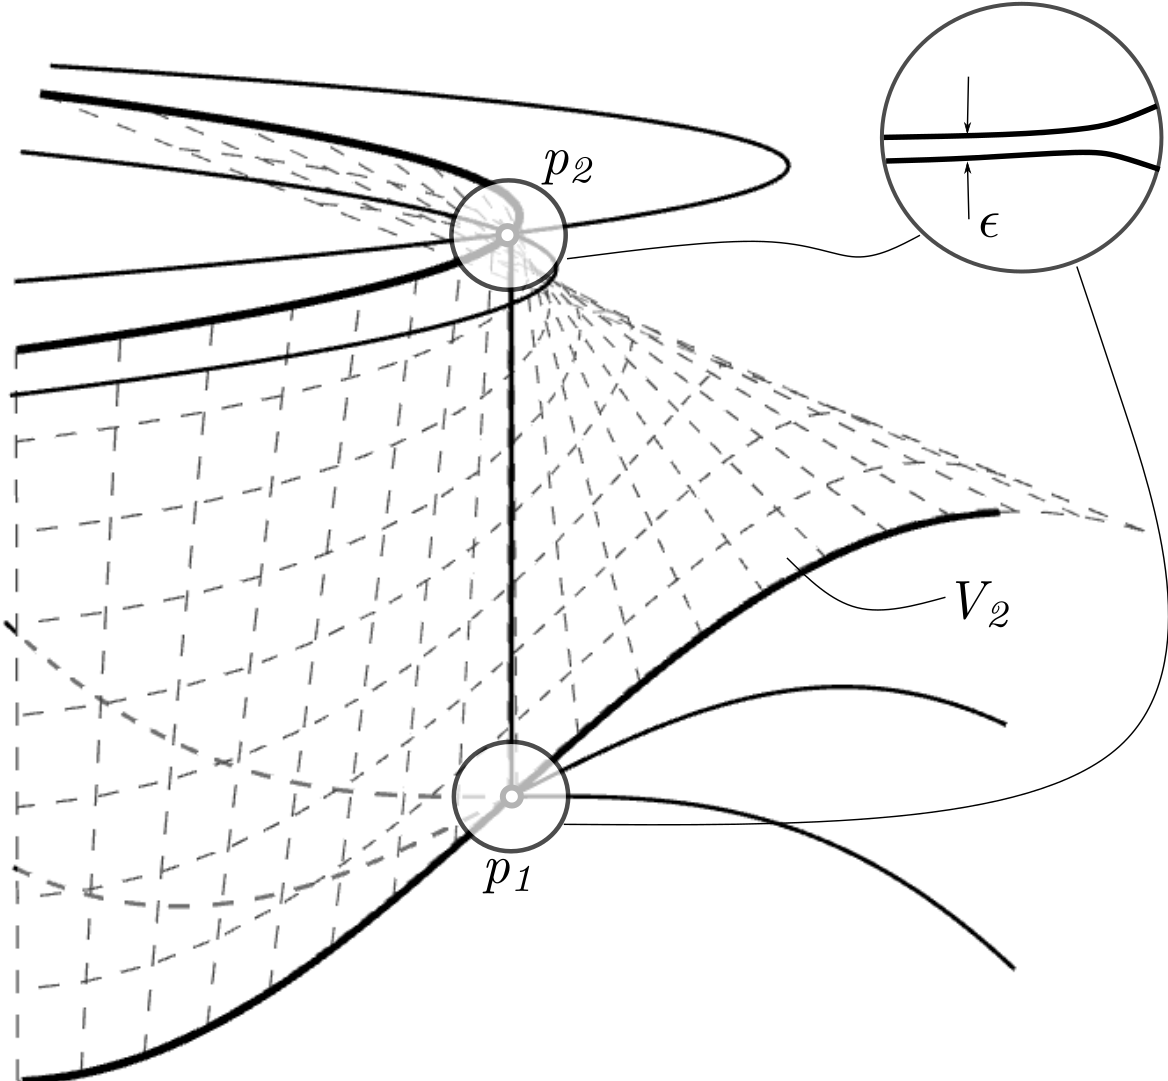
\includegraphics[width=6cm]{p87_c} }}%
        \qquad
    \subfloat[]{{\includegraphics[width=8cm]{p87_d} }}%
    %\caption{2 Figures side by side}%
    \label{fig:example}%
\caption{$V_2$ manifold of a family of geodesics}
\end{figure}
\begin{figure}[h]%
    \centering
\tdplotsetmaincoords{0}{10}
\pgfplotsset{every axis/.append style={
		scale=1,
		%axis lines=center,
		axis on top,
		xlabel={$x$},
		%ylabel={$z$},
               axis x line=middle,    % put the x axis in the middle
               axis y line=middle,    % put the y axis in the middle
               %x axis line style={-latex, ultra thin}, % arrows on the axis
               y axis line style={-,draw opacity=0},
                x axis line style={draw opacity=0},
            },}
            

            
\begin{tikzpicture}    [spy using outlines=	{circle, magnification=6, connect spies},] 
					
	\tikzmath{\u= 0.9;\w=-1.71;\v=1.0;\q= (2.0/ \w)*0.9994;\n=1;}
	\u,  \w, \v, \q, \n;
    \pgfplotsset{ticks=none};
    
    \pgfplotsset{compat=1.12};
		\def\r{0.5};
		\def\H{1.0};  
		\def\s{0.123};
	\begin{axis}
		[
		xmin=-0.7,
		xmax=0.7,
		ymin=-1.4,
		ymax=1.4,
		]
		%\addplot [black,thick,samples=1000,	samples y=0,	domain=-\r:\r,variable=\g]({ \r*(cos(\n*deg(2*ln(1-(\g)*\w/2))))},{(\u*(1-0.5*\g *\w)});
		%positve plane

		\addplot [decoration={markings,mark=at position 0.5 with {\arrow[scale=1,=>latex]{<}}},postaction={decorate}, black,thick,samples=60,	samples y=0,	domain=-\r:\r,variable=\g]({\g},{\u*(exp(0.5*(3.141593*(asin(\g/ \r)/360.-0.0))))});

		\addplot [black,dashed,thin,samples=40,	samples y=0,	domain=-\r:\r,variable=\g]({-\g},{\u*(exp(0.5*(3.141593*(asin(\g/ \r)/360.-0.5))))});
		%negative plane
		\addplot [decoration={markings,mark=at position 0.5 with {\arrow[scale=1.0,=>latex]{<}}},postaction={decorate},black,thick,samples=60,	samples y=0,	domain=-\r:\r,variable=\g]({\g},{-\u*(exp(0.5*(3.141593*(asin(\g/ \r)/360.-0.0))))});
		\addplot [black,dashed,thin,samples=40,	samples y=0,	domain=-\r:\r,variable=\g]({-\g},{-\u*(exp(0.5*(3.141593*(asin(\g/ \r)/360.-0.5))))});
		
		\foreach \k in {1,...,4}
{
%positve plane
  \addplot [black,very thick,samples=40,	samples y=0,	domain=-\r:\r,variable=\g]({\g},{\u*(exp(0.5*(3.141593*(asin(\g/ \r)/360.-\k ))))});
   \addplot [black,dashed,thin,samples=40,	samples y=0,	domain=-\r:\r,variable=\g]({-\g},{\u*(exp(0.5*(3.141593*(asin(\g/ \r)/360.-3*\k /2.))))});
  %negative plane
     \addplot [black,thick,samples=40,	samples y=0,	domain=-\r:\r,variable=\g]({\g},{-\u*(exp(0.5*(3.141593*(asin(\g/ \r)/360.-\k ))))});
   \addplot [black,dashed,thin,samples=40,	samples y=0,	domain=-\r:\r,variable=\g]({-\g},{-\u*(exp(0.5*(3.141593*(asin(\g/ \r)/360.-3*\k /2.))))});
}

      \coordinate (g1) at (axis cs:{\r*0.9},{\u*(exp(0.5*(3.141593*(asin(-\r/ \r)/360. +0.4))))});
      \coordinate (g2) at (axis cs:{\r*0.9},{-\u*(exp(0.5*(3.141593*(asin(-\r/ \r)/360.+0.4 ))))});
\node[tdplot_main_coords,{anchor=south east}] at (g1){$g_{1}$};
\node[tdplot_main_coords,{anchor=south east}] at (g2){$g_{2}$};

\foreach \j in {1,..,3}
{
%\draw (\j,0) -- (\j,\H*1.3);
}
\draw[very thin,] (\r,-\H*1.3) -- (\r,\H*1.3);
\draw[very thin,] (-\r,-\H*1.3) -- (-\r,\H*1.3);
\draw[thick,gray!60] (-\r,0) -- (\r,0);
\draw[very thin,black] (-\r,0) -- (\r,0);
\draw[very thin,black] (-\r*1.2,0) -- (-\r,0);
\draw[very thin,black,- stealth] (\r,0) -- (\r*1.42,0);


		%using the 'spy' to magnify a piece of the picture
  % now we can draw the magnifying glass:
    %\spy [black] on (2.84,2.87) in node [left] at (2.25,1.6);
      \coordinate (spypoint) at (axis cs:-0.493,0);
  \coordinate (magnifyglass) at (axis cs:-0.8,0.6);
\end{axis}
\spy [black, size=2.5cm] on (spypoint)   in node[fill=white] at (magnifyglass);

\end{tikzpicture}
\caption{$V_2$ Misner cylinder family of geodesics}
\end{figure}
$$\blacklozenge$$
\newpage

\end{comment}
\chapter{Special types of space}
\pagebreak[4]
\section{p112 - Exercise}
\begin{tcolorbox}
Deduce from $4.110.$ that the Gaussian curvature of a $V_2$ positive-definite metric is given by $$ G = \frac{R_{1212}}{a_{11}a_{22}-a_{12}^2}$$
\end{tcolorbox}
From p. 86 (exercise) we know that all the components of $R_{mnrs}$ can be expressed as terms of $R_{1212}$ (or vanish). \\
So by $4.110.$, 
\begin{align}
K\left({a_{11}a_{22}-a_{12}a_{21}}\right) = R_{1212}
\end{align}
and from page 96 $\mathbf{(3.415)}$ we know that for $V_2$, $K=G$. Hence,
\begin{align}
G = \frac{R_{1212}}{\left(a_{11}a_{22}-a_{12}a_{21}\right)}
\end{align}
$$\blacklozenge$$
\newpage

\section{p113 - Exercise}
\begin{tcolorbox}
Prove that, in a space $V_N$ of constant curvature $K$,$$\mathbf{(4.115)}\spatie R_{mn} = -\left(N-1\right)Ka_{mn}, \quad R = -N\left(N-1\right)K$$
\end{tcolorbox}
We have
\begin{align*}
R_{mn} = R^s_{.mns} = a^{sk}R_{kmns}
\end{align*}
From $\mathbf{(4.114)}$
\begin{align*}
&R_{kmns} = K\left(a_{kn}a_{ms}-a_{ks}a_{mn}\right)\\
\Rightarrow\spatie &R_{kmns}= K \left(\underbrace{\delta^s_n a_{ms}}_{a{mn}}-Na_{mn}\right)= K\left(1-N\right)a_{mn}
\end{align*}
and 
\begin{align*}
R &= R^n_{.n}\\
&= a^{kn}R_{kn}\\
&= -\underbrace{a^{kn}a_{kn}}_{N}\left( N-1 \right)K\\
&= -N\left( N-1 \right)K
\end{align*}
$$\blacklozenge$$
\newpage

\section{p113 - Clarification}
\begin{tcolorbox}
$$\mathbf{4.117.}\spatie \frac{\delta^2 \eta^r}{\delta s^2} + \epsilon K\eta^r =0$$
\end{tcolorbox}
We have
\begin{align}
R^r_{.smn} &= a^{rk} R_{ksmn}\\
\text{(4.114)}\Rightarrow \spatie &= a^{rk} K\left(a_{km}a_{sn}-a_{kn}a_{sm}\right)\\
&= K\left(\delta^r_m a_{sn}-\delta^r_n a_{sm}\right)
\end{align}
\begin{align*}
\text{(3.311) and (3)}\spatie 0 &=\frac{\delta^2 \eta^r}{\delta s^2} +  K\left(\delta^r_m a_{sn}-\delta^r_n a_{sm}\right)p^s\eta^m p^n\\
\Leftrightarrow\spatie 0 &=\frac{\delta^2 \eta^r}{\delta s^2} +  K\left(\delta^r_m \eta^m \underbrace{a_{sn}p^s p^n}_{=\epsilon}-\delta^r_n \underbrace{a_{sm}p^s\eta^m}_{=0} p^n\right)\\
\Leftrightarrow\spatie 0 &=\frac{\delta^2 \eta^r}{\delta s^2} +  K\epsilon\underbrace{\delta^r_m \eta^m}_{=\eta^r} \\
\Leftrightarrow\spatie 0 &=\frac{\delta^2 \eta^r}{\delta s^2} +  K\epsilon\eta^r
\end{align*}
$$\blacklozenge$$
\newpage

\section{p114 - Clarification}
\begin{tcolorbox}
$$\mathbf{4.118.}\spatie \dv[2]{\left(X_r\eta^r\right)}{s} + \epsilon K\left(X_r\eta^r\right) =0$$
\end{tcolorbox}
We know that $\frac{\delta X_r}{\delta s} = 0$ (parallel transport)
\begin{align*}
&\frac{\delta \left(X_r\eta^r\right)}{\delta s}= \eta^r\underbrace{\frac{\delta X_r}{\delta s}}_{=0}+X_r\frac{\delta \eta^r}{\delta s}\\
\Rightarrow\spatie &\frac{\delta^2 \left(X_r\eta^r\right)}{\delta s}= \underbrace{\frac{\delta X_r}{\delta s}}_{=0}\frac{\delta \eta^r}{\delta s}+X_r\frac{\delta^2 \eta^r}{\delta s^2}\\
\Rightarrow\spatie &X_r\frac{\delta^2 \eta^r}{\delta s^2}= \frac{\delta^2 \left(X_r\eta^r\right)}{\delta s^2}\\
\text{but}\spatie &\frac{\delta^2 \left(X_r\eta^r\right)}{\delta s^2} =  \dv[2]{X_r\eta^r}{s} \quad \text{ as } X_r\eta^r \text{ is an invariant}\\
\Rightarrow \spatie &X_r\frac{\delta^2 \eta^r}{\delta s^2}=\dv[2]{X_r\eta^r}{s}\\
\text{and so}\spatie &\frac{\delta^2 \left(\eta^r\right)}{\delta s^2}X_r + \epsilon K\left(X_r\eta^r\right) = \dv[2]{X_r\eta^r}{s}+ \epsilon K\left(X_r\eta^r\right) = 0
\end{align*}
$$\blacklozenge$$
\newpage

\section{p115 - Exercise}
\begin{tcolorbox}
By taking an orthonormal set of $N$ unit vectors propagated parallely along the geodesic, deduce from $4.120a$ that the magnitude $\eta$ of the vector $\eta^r$ is given by $$ \eta = C\left|\sin \left(s\sqrt{\epsilon K}\right)\right|$$ where $C$ is a constant.
\end{tcolorbox}
We have by $4.120a$
\begin{align}
X_r \eta^r &= A\sin \left(s\sqrt{\epsilon K}\right)
\end{align}
We choose $N$ different $X^{(k)}_r$ $(k= 1,2,\dots, N)$ which are orthonormal.
Applying $(1)$ $N$ times with the different $X^{(k)}_r$ $(k= 1,2,\dots, N)$, we get
\begin{align}
X^{(k)}_r \eta^r &= A^{(k)}\sin \left(s\sqrt{\epsilon K}\right)
\end{align}
But as the $X^{(k)}_r$ are orthonormal and are used as a basis at the considered point of the geodesic we have 
\begin{align*}
X^{(k)}_r &= \delta^k_r
\end{align*}
So, $(2)$ becomes
\begin{align*}
\eta^k &= A^{(k)}\sin \left(s\sqrt{\epsilon K}\right)
\end{align*}
which are the components of the displacement vector in the orthonormal basis. By $\mathbf{2.301.}$ :
\begin{align*}
Y^2 &= \epsilon a_{mn} Y^m Y^n\\
\Rightarrow \spatie \eta^2 &= \epsilon a_{mn} A^{(m)} A^{(n)}\sin^2 \left(s\sqrt{\epsilon K}\right)\\
\Rightarrow \spatie \eta &= C\left|\sin \left(s\sqrt{\epsilon K}\right)\right|\\
\text{with}\spatie C&= \sqrt{\left|\epsilon a_{mn} A^{(m)} A^{(n)}\right|}
\end{align*}
$$\blacklozenge$$
\newpage

\section{p118 - Exercise}
\begin{tcolorbox}
Examine the limit of the form $\mathbf{4.130}$ as $R$ tends to infinity, and interpet the result.
\end{tcolorbox}
We have $$\mathbf{4.130.}\spatie ds^2 = dr^2+R^2\sin^2\left(\frac{r}{R}\right)\left(d\theta^2 + \sin^2\theta d\phi^2\right)$$
But $\sin \epsilon \approx \epsilon$ for $\epsilon  \ll 1$. So
\begin{align}
 \lim_{R\rightarrow \infty} ds^2 &= dr^2+R^2\left(\frac{r}{R}\right)^2\left(d\theta^2 + \sin^2\theta d\phi^2\right)\\
 &= dr^2+\left(r d\theta^2 \right) + \left(r\sin\theta d\phi\right)^2
 \end{align}
 This is the metric form for an Euclidean 3-space with spherical polar coordinates (see $\mathbf{2.532.}$ page 54).
$$\blacklozenge$$
\newpage

\section{p119 - Exercise}
\begin{tcolorbox}
Show that a transformation of a homogeneous coordinate system  into another homogeneous system is necessarily linear. (Use the transformation equation $\mathbf{2.507}$ for Christoffel symbols, noting that all Christoffel symbols vanish  when the coordinates are homogeneous).
\end{tcolorbox}
By $2.507$ we have the transformation rule 
\begin{align}
\Gamma^{'a}_{bc} = \Gamma^{r}_{mn}\partial_r z^a\partial_b z^m \partial_c z^n + \partial_r z^a\frac{\partial^2 z^r}{\partial z^b \partial z^c} 
\end{align}
But, as both coordinate system are homogeneous, all Christoffel symbols vanish and so
\begin{align}
\Gamma^{'a}_{bc} = \partial_r z^a\frac{\partial^2 z^r}{\partial z^b \partial z^c} &=0\\
\Rightarrow \spatie \partial_r z^a\frac{\partial^2 z^r}{\partial z^b \partial z^c} &=0
\end{align}
As the Jacobian can't vanish the possibility of having $\partial_r z^a=0$ $\forall a, r$ is excluded. Hence we must have $\frac{\partial^2 z^r}{\partial z^b \partial z^c} =0$. And have a linear solution of the form
\begin{align}
z^r = A_k z^{'k}+C
\end{align}
$$\blacklozenge$$
\newpage

\section{p120 - Exercise}
\begin{tcolorbox}
If $z_r, z^{'}_r$ are two systems of rectangular Cartesian coordinates in Euclidean 3-space, what is the geometrical interpretation of the constants in $\mathbf{4.204}$ and of the orthogonality conditions $\mathbf{4.209}$ ?
\end{tcolorbox}
We have 
\begin{align}
z^{'}_m &= A_{mn}z_n+A_m 
\end{align}
As we assume that the Jacobian of the transformation does not vanish and thus the mapping is bijective, in an Euclidean 3-space $A_m$ will perform a $\mathit{translation}$ while $A_{mn}$ can be interpreted as a combination rotation/reflection/stretching/contraction/shearing. I.e. the mapping is an $\mathit{affine}$ transformation.\\
The condition $\mathbf{4.209}$ restricts the action of $A_{mn}$ to a combination of rotation/reflection. Indeed, a rotation/reflection can be represented by $R= R_x\left(\gamma\right) \circ R_y\left(\beta\right)\circ  R_z\left(\alpha\right)$ with 
\begin{align}
R_x = \begin{pmatrix}
\pm 1&0  &0  \\
0&\cos\gamma & -\sin\gamma \\
 0&\sin\gamma & \cos\gamma   \\
\end{pmatrix}
R_y = \begin{pmatrix}
\cos\beta & 0& -\sin\beta \\
 0& \pm 1&0 \\
 \sin\beta & 0& \cos\beta\\
\end{pmatrix}
R_z = \begin{pmatrix}
\cos\alpha & -\sin\alpha  & 0 \\
 \sin\alpha & \cos\alpha  & 0 \\
  0&0  & \pm 1 \\
\end{pmatrix}
\end{align}
Note that for every axis, $R_k^{T} R_k^{} = \mathbb{I}_3$.\\
Be $A_{mn} = R_x\left(\gamma\right) \circ R_y\left(\beta\right)\circ  R_z\left(\alpha\right)$
We have by $\mathbf{4.209}$, $A_{mq}A_{mq}= \delta_{pq}$ which can be expressed as 
\begin{align}
A^{T}A &= \mathbb{I}_3\\
\Rightarrow \spatie \mathbb{I}_3 &= \left( R_x R_y R_z\right)^T R_xR_yR_z\\
&=  \underbrace{R_z^T \underbrace{R_y^T\underbrace{R_x^TR_x}_{= \mathbb{I}} R_y}_{= \mathbb{I}}R_z}_{= \mathbb{I}_3}
\end{align}
The identity yields, and interpret the coefficients of the orthogonal transformation as an Euclidean orthogonal transformation. 
$$\blacklozenge$$
\newpage

\section{p123 - Clarification}
\begin{tcolorbox}
If $A_{n}A_{n} =0$ it follows from $\mathbf{2.445}$ and $\mathbf{2.446}$ that the straight line is a geodesic null line.
\end{tcolorbox}
We have 
\begin{align}
\text{(2.446)}\spatie & a_{mn}\dv{x^m}{u}\dv{x^n}{u}=0 \spatie \dv{x^m}{u}= \dv{z_m}{u} = A_m\\
\text{(4.215)}\spatie & a_{mn}=\delta_{mn}\\
\text{(1),(2) \ }\Rightarrow \spatie &\delta_{mn}\dv{z_m}{u}\dv{z_n}{u}=0\\
\Rightarrow \spatie &A_nA_n=0
\end{align}
$$\blacklozenge$$
\newpage


\section{p123 - Clarification}
\begin{tcolorbox}
It is easy to see ... viz., $$\mathit{the \ straight \ line \ joining \ any \ two \ points \ in \ a \ plane \ lies \ entirely \ in \ the \ plane.}$$ 
\end{tcolorbox}
The plane is identified by 
\begin{align*}
A_n z_n+B=0
\end{align*}
and a line by
\begin{align*}
z_n = C_nu+D_n
\end{align*}
Take two points at $u=0$ and $u=p$ lying in the plane:
\begin{align*}
& \left\{ \begin{array}{l}
A_nC_np+A_nD_n+B=0\\
A_nD_n+B=0
\end{array} \right.\\
\Rightarrow\spatie & \left\{ \begin{array}{l}
A_nC_np=0\\
A_nD_n+B=0
\end{array} \right.
\end{align*}
And as $p\neq 0 \ \Rightarrow A_nC_n = 0$. So for any arbitrary $u$ of this line we have
\begin{align*}
\underbrace{A_nC_n}_{=0}u+\underbrace{A_nD_n+B}_{=0}=0
\end{align*}
hence, all points of the line lie in the plane.
$$\blacklozenge$$
\newpage


\section{p123 - Exercise}
\begin{tcolorbox}
Show that a one-flat is a straight line.
\end{tcolorbox}
A one-flat means $(N-1)$ equations 
\begin{align}
A^{(k)}_nz_n + B^{(k)} =0 \quad k=1,\dots,N-1\quad n= 1,\dots,N
\end{align}
This is a set of $(N-1)$ linear equation in $N$ unknown $z_n$. So we have one degree of freedom.\\
E.g. put $z_N=u$ with u the free parameter. then,
\begin{align}
A^{(k)}_{\alpha}z_{\alpha}+ A^{(k)}_{N}u+ B^{(k)} =0 \quad \alpha=1,\dots,N-1
\end{align}
If $detA^{(k)}_{\alpha} \neq0$ we get a solution of the set of equation
\begin{align}
Az&=B \quad\text{with}\quad B \text{ a linear function in } u\\
\Rightarrow\spatie z_m&= \left(A^{-1}B\right)_m
\end{align}
with $\left(A^{-1}B\right)_m$ of the form $C_mu+D_m$
$$\blacklozenge$$
\newpage

\section{p126 - Exercise$\dagger$}
\begin{tcolorbox}
Show that the null cone with vertex at the origin in space-time has the equation $$\mathbf\spatie y^2_1+y^2_2+y^2_3-y^2_4=0$$
Prove that this null cone divides space-time into three regions such that \\
$\mathit{a.}$ Any two points (events) both lying in one region can be joined by a continuous curve which does not cut the null cone.\\
$\mathit{b.}$ All continuous curves joining two given points (events) which lie in different regions, cut the null cone.\\
Show further that the three regions may be further classified into past, present, and future as follows: If $A$ and $B$ are any two points in the past, then the straight segment $AB$ lies entirely in the past. If $A$ and $B$ are any two points in the future, then the straight segment $AB$ lies entirely in the future. If $A$ is any point in the present, there exist at least one point $B$ in the present that the straight segment $AB$ cuts the null cone.
\end{tcolorbox}

We first prove 
$$\mathbf\spatie y^2_1+y^2_2+y^2_3-y^2_4=0$$
The null geodesic equations:
\begin{align*}
& \left\{ \begin{array}{l}
\frac{\delta^2 x^r}{\delta u^2} = \dv[2]{x_r}{u} =0 \quad \text{ as we use homogeneous coordinates}\\\\
a_{mn} \dv{x_m}{u}\dv{x_n}{u}=0\\
\end{array} \right.\\
\Rightarrow \spatie & \left\{ \begin{array}{l}
x_r = A_ru+B_r\quad \text{( put } B_r=0 \text{ by adequate choice of the origin )} \\\\
A_1^2+A_2^2+A_1^2+A_3^2-A_4^2=0\\
\end{array} \right.\\
\Rightarrow \spatie &\frac{\left((x_1)^2+(x_2)^2+(x_3)^2-(x_4)^2\right)}{u^2} = 0\quad \text{ for } u\neq 0\\
\Rightarrow \spatie &(x_1)^2+(x_2)^2+(x_3)^2-(x_4)^2 = 0
\end{align*}
$$\lozenge$$
About the existence of three regions. First let's investigate the case in a $V_3$ space-time manifold in order to have a more intuitive grasp.\\
Consider a family of events $(p_1,p_2,u)$ with $u\in\left(-\infty,\infty\right)$ (see the line $P^{'}P^{"}$ in figure 1.1.)
\begin{figure}[H]
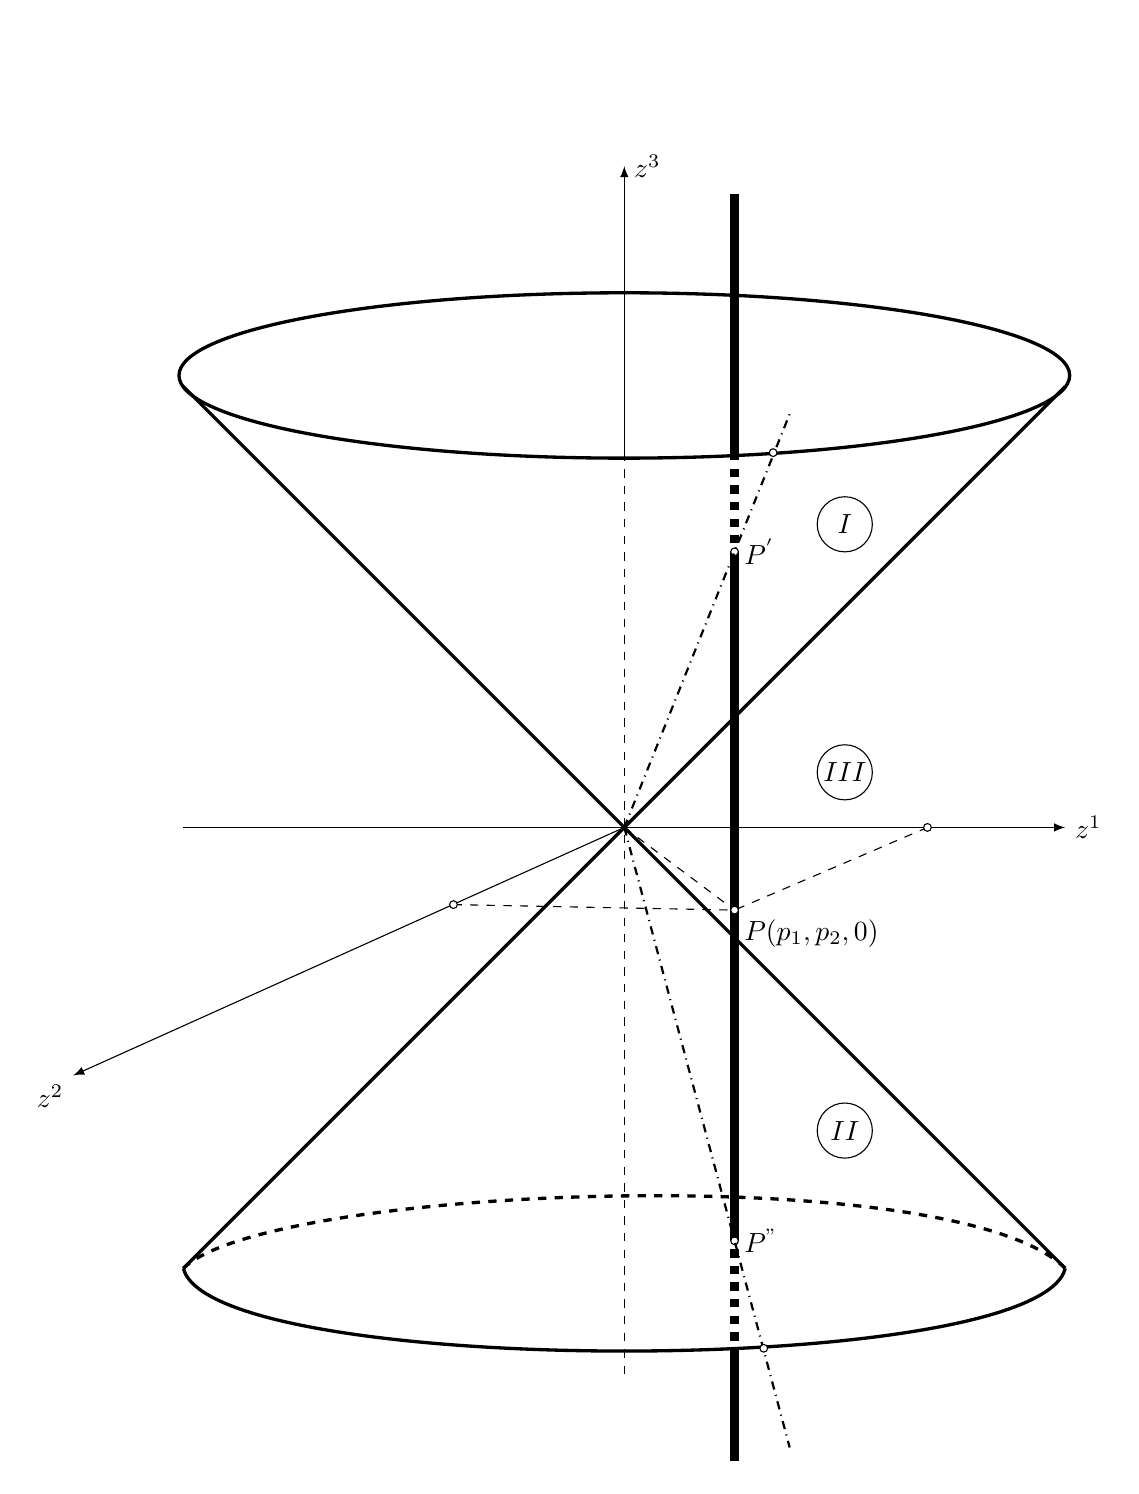
\begin{tikzpicture}[scale=0.70]
\coordinate (v1) at (-8,-0);
\coordinate (v2) at (8,-0) ;
\coordinate (v3) at (0,12) {};
\coordinate (v4) at (0,6.8) {};
\coordinate (v5) at (8,8) {};
\coordinate (v6)  at (0,0) {};
\coordinate (v7) at (-8,-8) {};
\coordinate (v8) at (8,-8) {};
\coordinate (v9) at (-8,8) {};
\coordinate (v10) at (-0,-10) {};
\coordinate (v11)  at (-10,-4.5) {};
\draw[-{latex}]  (v1)-- (v2)node[right] {$z^1$};
\draw  [-{latex}](v4)-- (v3)node[right] {$z^3$};
\draw  [-{latex}](v6)-- (v11)node[{anchor=north east}] {$z^2$};
\draw  [dashed](v4)-- (v10);
\draw[very thick]  (0,8.2) ellipse (8.08 and 1.5);
\draw [very thick] (v6) -- (v5);
\draw [very thick] (v7) -- (v6);
\draw  [very thick](v6) -- (v8);
\draw  [very thick](v6) -- (v9);
\draw[very thick] (-8,-8) .. controls (-7.5,-10) and (7.5,-10) .. (8,-8);
\draw [very thick, dashed,](-8,-8) .. controls (-6.5,-6.5) and (6,-6) .. (8,-8);

\coordinate (p0) at (-3.1,-1.4) {} {};
\coordinate (p1) at (2,-1.5) {} {};
\coordinate (p2) at (2,5) {} {};
\coordinate (p3) at (2,-7.5) {} {};
\coordinate (p4) at (5.5,0) {};
\draw [dashed, thin] (p0) -- (p1);
\draw [dashed, thin] (p4) -- (p1);
\draw [dashed, thin] (v6) -- (p1);
\draw [line width=3] (p2) -- (p1);
\draw [line width=3] (p2) -- (p3);
\coordinate (p5) at (2,6.7) {};
\coordinate (p6) at (2,-9.5) {};
\coordinate (p7)at (2,11.5) {};
\coordinate (p8)  at (2,-11.5) {};
\draw [dashed, line width=3] (p3) -- (p5);
\draw  [dashed, line width=3] (p2) -- (p6);
\draw [ line width=3] (p7) -- (p5);
\draw[ line width=3] (p8) -- (p6);
\draw[fill=white](p0) circle(2pt);
\draw[fill=white](p4) circle(2pt);
\draw[fill=white](p3) circle(2pt)node[{anchor=west }] {$P^{"}$};
\draw[fill=white](p2) circle(2pt)node[{anchor=west }] {$P^{'}$};
\draw[fill=white](p1) circle(2pt)node[{anchor=north west }] {$P(p_1,p_2,0)^{}$};
\coordinate (p9)  at (1.5*2,-1.5*7.5) {};
\coordinate (p10)  at (1.5*2,1.5*5) {};
\draw  [dashdotted,thick](v6) edge (p9);
\draw  [dashdotted,thick](v6) edge (p10);
\coordinate (t1) at (4,5.5) {};
\coordinate (t2) at (4,1) {} ;
\coordinate (t3) at (4,-5.5) {};
\draw[fill=black](t1)node[] {$I$};
\draw[fill=black](t2)node[] {$III$};
\draw[fill=black](t3)node[] {$II$};
\coordinate (t4) at (2.7,6.8) {};
\coordinate (t5) at (2.53,-9.45) {};
\draw[fill=white](t4) circle(2pt);
\draw[fill=white](t5) circle(2pt);

\draw  (t1) ellipse (0.5 and 0.5);
\draw  (t2) ellipse (0.5 and 0.5);
\draw  (t3) ellipse (0.5 and 0.5);
\draw  (-1.5,14.5) ellipse (0 and 0);
\end{tikzpicture}
\caption{Regions delimited by the light cone in a $V_3$ space-time manifold}
\label{fig:fig_p96_3415_a}
\end{figure}
Be $R^2 = y_1^2 +y_2^2$. The light cone has the the equation $R^2- y_3^2=0$. Only the events at $ u_0 = \pm R(p_1,p_2)$ will lie on the light-cone.\\
We can distinguish three regions:\\
Region I where $u > u_0 = R$: the events $(p_1,p_2,u)$ will lie on the line above point $P^{'}$.\\
Region II where $ u < -u_0 = -R$: the events $(p_1,p_2,u)$ will lie on the line below point $P^{"}$.\\
Region III where $ -R= -u_0 < u < u_0 = R$: the events $(p_1,p_2,u)$ will lie on the segment $P^{'}P^{"}$.\\
Let's generalize this now for a $V_4$ space-time manifold.\\
Put $R^2 = (y_1)^2+(y_2)^2+(y_3)^2$ and consider $\phi(y_1,y_2,y_3,y_4)= (y_1)^2+(y_2)^2+(y_3)^2-(y_4)^2$ so \begin{align}\phi(y_1,y_2,y_3,y_4)= R^2-(y_4)^2\end{align}
For $\phi=0$ we lie on the light-cone.\\
For $\phi>0 \quad\Rightarrow R^2 > y_4^2$ and so $-R<y_4<R$ defines one region (region III).\\
For $\phi<0 \quad\Rightarrow R^2 < y_4^2$ and so   $y_4>R$ or $y_4<-R$ define two  regions (region I and II).
$$\lozenge$$

\textbf{We now show statement $\mathit{a.}$ of the exercise.}\\
Consider $2$ events $P_0,\ P_1$ with coordinates $(y_1^{(0)},y_2^{(0)},y_3^{(0)},y_4^{(0)})$ and $(y_1^{(1)},y_2^{(1)},y_3^{(1)},y_4^{(1)})$  and a curve defined by 
\begin{align}
y_i= \pm\sqrt{\left(\left(y_i^{(1)}\right)^2-\left(y_i^{(0)}\right)^2\right)u + \left(y_i^{(0)}\right)^2}\spatie u\in \left[0,1\right]
\end{align}
where the $\pm$ is chosen so that $y_i(0) = y_i^{(0)}$ and $y_i(1) = y_i^{(1)}$ and that the sign only changes when $y_i(u)=0$ and $sign\left(y_i^{(0)}\right) \neq sign\left(y_i^{(1)}\right)$. Such curve will be continuous.\\
Be $\phi_0\equiv \phi(0)$, $\phi_1\equiv \phi(1)$,

Then $(2)$ in $(1)$ gives
\begin{align}
&\phi(u) = \left(\phi_1-\phi_0\right)u+\phi_0
\end{align}\\\\
\textit{Case a1: $P_0, P_1$ both lie in region I or both in region II.} \\
We have the following conditions:
\begin{align*}
\phi_0 < 0\wedge \phi_1  < 0
\end{align*}
then, $$\cancel{\exists } \  u \in \left[0,1\right]: \phi(u)=0$$
 Indeed, put $\tau = -\phi_0 \text{ and }  \sigma =-\phi_1  $ with $\tau,\ \sigma>0$. Then, from $(3)$ we deduce that for  $\phi(u)=0$ we get 
 \begin{align}
 &u= -\frac{\phi_0}{\phi_1-\phi_0}\\
 \Rightarrow\spatie & u= \frac{\tau}{\tau-\sigma}\\
 \Rightarrow\spatie & u= \frac{1}{1-\frac{\sigma}{\tau}}\\
 \Rightarrow\spatie &\cancel{\exists}  \  u \in \left[0,1\right]: \phi(u)=0 \spatie \text{ as } \frac{\sigma}{\tau} >0
 \end{align}
So, there exist no $u\in\left[0,1\right]$ for which $\phi(u)=0$ and the curve does not intersect the null cone.\\\\
\textit{Case a2: $P_0, P_1$ both lie in region III.} Then,
\begin{align*}
\phi_0 > 0\wedge \phi_1  > 0
\end{align*}
Following the same reasoning as in $(7)$ but with $\tau = \phi_0 \text{ and }  \sigma =\phi_1  $ with $\tau,\ \sigma >0$ we can conclude
$$\cancel{\exists } \  u \in \left[0,1\right]: \phi(u)=0$$ 
So, there exist no $u\in\left[0,1\right]$ for which $\phi(u)=0$ and the curve does not intersect the null cone.\\\\
\\$$\lozenge$$

\textbf{We now show statement $\mathit{b.}$ of the exercise.}\\\\
\begin{comment}
\textit{Case b1: $P_0$ lies in region I, $P_1$  lies in region II.} \\
Those two regions are separated by the $3$-flat (plane) $y_4=0$. So it's suffice that $R^2=0$ for $\phi(u)$ being zero. Hence $y_i=0$, $  i=1,2,3$, and the curve will cut the cone at it's apex.
\\\\
\textit{Case b2: $P_0$ lies in region I or II, $P_1$  lies in region III.} \\
Put
\begin{align*}
R^2&= \left(y_1\right)^2+\left(y_2\right)^2+\left(y_3\right)^2\\
{R_{0}}^2&= \left(y^0_1\right)^2+\left(y^0_2\right)^2+\left(y^0_3\right)^2\\
{R_{1}}^2&= \left(y^1_1\right)^2+\left(y^1_2\right)^2+\left(y^1_3\right)^2
\end{align*}
For the points on the curve, $R^2$ can then be written as 
\begin{align*}
R^2&= \left(R_1^2-R_0^2\right)u+R_0^2
\end{align*}
Then \begin{align}
&\phi(u) = \left(R_1^2-R_0^2\right)u+R_0^2 - \left[\left(y_4^{(1)}\right)^2   -\left(y_4^{(0)}\right)^2 \right]u -\left(y_4^{(0)}\right)^2 \quad \text{(see (1))}
\end{align}\\
We have the following conditions:\\
\begin{align*}
\left\{\begin {matrix}
\phi_0 < 0&\wedge &\phi_1  > 0\\\\
R_0^2 > (y_4^{0})^2&\wedge & R_1^2 < (y_4^{1})^2
\end{matrix}\right.
\end{align*}
Then, $$\exists  \  u \in \left[0,1\right]: \phi(u)=0$$
 From $(4)$ we have ,
\begin{align}
\phi(u)=0\quad\Rightarrow\spatie  &= -\frac{R_0^2- \left(y_4^{(0)}\right)^2}{R_1^2-R_0^2  -\left(y_4^{(1)}\right)^2  +\left(y_4^{(0)}\right)^2}
\end{align}

Let's simplify notationally the last equation. As $\phi_0 < 0\wedge \phi_1 > 0$, put $R_0^2- \left(y_4^{(0)}\right)^2=-\tau $ and $R_1^2- \left(y_4^{(1)}\right)^2=\sigma$ with both $\tau, \sigma > 0$. $(5)$ can be written as
\begin{align*}
u&=\frac{\tau}{\sigma +\tau}\\
 &=\frac{1}{1+\frac{\sigma}{\tau}}\\
\Rightarrow\spatie &\exists  \  u \in \left[0,1\right]: \phi(u)=0 \spatie \text{ as } \frac{\sigma}{\tau} >0
\end{align*}
So, there is a solution $u\in \left[0,1\right]$ for which $\phi(u)=0$ and the curve intersects the null cone.
\end{comment}
$$\dagger$$
\\$$\lozenge$$\\


\textbf{We now investigate the straight segment questions.} \\
\begin{comment}
\textit{Case 1: $A$ and $B$ both lie in the present (region I) or in the past (region II)}\\\\
\\\\

\textit{Case 2: If $A$ is any point in the present, there exist at least one point $B$ in the present that the straight segment $AB$ cuts the null cone}\\\\

\end{comment}










\begin{comment}
Then,
 \begin{align}
\phi(u) &= \left\{\begin{array}{l} \ \ \left[\left(y_1^{(1)}-y_1^{(0)}\right)u + y_1^{(0)}\right]^2\\
+\left[\left(y_2^{(1)}-y_2^{(0)}\right)u + y_2^{(0)}\right]^2\\
+\left[\left(y_3^{(1)}-y_3^{(0)}\right)u + y_3^{(0)}\right]^2\\
-\left[\left(y_4^{(1)}-y_4^{(0)}\right)u + y_4^{(0)}\right]^2\\
\end{array}\right.\\
&= \left\{\begin{array}{l} \ \ 
\left(y_1^{(1)}\right)^2 u^2+\left(y_1^{(0)}\right)^2 u^2 - 2y_1^{(1)}y_1^{(0)}u^2 + 2y_1^{(1)}y_1^{(0)}u-  2\left(y_1^{(0)}\right)^2 u+ \left(y_1^{(0)}\right)^2\\
+\left(y_2^{(1)}\right)^2 u^2+\left(y_2^{(0)}\right)^2 u^2 - 2y_2^{(1)}y_2^{(0)}u^2 + 2y_2^{(1)}y_2^{(0)}u-  2\left(y_2^{(0)}\right)^2 u+ \left(y_2^{(0)}\right)^2\\
+\left(y_3^{(1)}\right)^2 u^2+\left(y_3^{(0)}\right)^2 u^2 - 2y_3^{(1)}y_3^{(0)}u^2 + 2y_3^{(1)}y_3^{(0)}u-  2\left(y_3^{(0)}\right)^2 u+ \left(y_3^{(0)}\right)^2\\
-\left(y_4^{(1)}\right)^2 u^2-\left(y_4^{(0)}\right)^2 u^2 + 2y_4^{(1)}y_4^{(0)}u^2 - 2y_4^{(1)}y_4^{(0)}u+  2\left(y_4^{(0)}\right)^2 u- \left(y_4^{(0)}\right)^2\\
\end{array}\right.
\end{align}
Put $\phi_0 = \left(y_1^{(0)}\right)^2+\left(y_2^{(0)}\right)^2+\left(y_3^{(0)}\right)^2-\left(y_4^{(0)}\right)^2$ and $\phi_1 = \left(y_1^{(1)}\right)^2+\left(y_2^{(1)}\right)^2+\left(y_3^{(1)}\right)^2-\left(y_4^{(1)}\right)^2$. \\
Then,
\begin{align}
\phi(u)= \left\{\begin{array}{l} \ \ 
\phi_1u^2+\phi_0u^2-2\left(y_1^{(1)}y_1^{(0)}+y_2^{(1)}y_2^{(0)}+y_3^{(1)}y_3^{(0)}-y_4^{(1)}y_4^{(0)}\right)u^2 \\
-2\phi_0 u + 2 \left(y_1^{(1)}y_1^{(0)}+y_2^{(1)}y_2^{(0)}+y_3^{(1)}y_3^{(0)}-y_4^{(1)}y_4^{(0)}\right)u\\
+\phi_0
\end{array}\right.
\end{align}
Let's put $\kappa = y_1^{(1)}y_1^{(0)}+y_2^{(1)}y_2^{(0)}+y_3^{(1)}y_3^{(0)}-y_4^{(1)}y_4^{(0)}$, we get the expression
\begin{align}
\phi(u)&= 
\left(\phi_1 +\phi_0-2\kappa\right) u^2 + 2 \left(\kappa- \phi_0\right)u
+\phi_0
\end{align}


The function $\phi(u)$ is a parabola. 
\begin{figure}[H]%
    \centering
    \subfloat[]{
       


            
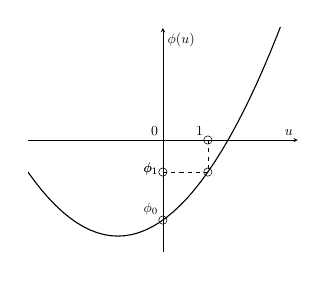
\begin{tikzpicture} [scale=0.5,c/.style={insert path={circle[radius=3pt]}}] 
\pgfplotsset{every axis/.append style={
		scale=1,
		axis lines=center,
		axis on top,
		xlabel={$u$},
		ylabel={$\phi(u)$},
               axis x line=middle,    % put the x axis in the middle
               axis y line=middle,    % put the y axis in the middle
               %x axis line style={-latex, ultra thin}, % arrows on the axis
               y axis line style={draw opacity=1},
                x axis line style={draw opacity=1},
            }}
     
					
	\tikzmath{\u=5;\a=0.2;\b=2*\a;\d=-1;}
	 \u,\a, \b,\d;
    \pgfplotsset{ };
    
    \pgfplotsset{compat=1.12};
		\def\r{3};
		\def\H{1.0};  
		\def\s{0.123};
	\begin{axis}
		[
		xmin=-3,
		xmax=3,
		ymin=-1.4,
		ymax=1.4,
		xminorticks=true,
		yminorticks=false,
		ytick=\empty,
		xtick=\empty,
		]

		\addplot [black,thick,samples=40,samples y=0,	domain=-\r:\r,variable=\u]({\u},{\a*\u^2+\b*\u+\d});
		%\addplot [black,thick,samples=40,samples y=0,	domain=-\r:\r,variable=\u]({\u},{10*\a*\u^2+\b*\u+\d});

	\coordinate (x0) at ({0},{0});
	\coordinate (x1) at ({1},{0});
	\coordinate (p1) at ({1},{\a+\b+\d});
	\coordinate (p1y) at ({0},{\a+\b+\d});
	\coordinate (p1x) at ({1},{0});
	\coordinate (p2) at ({1},{10*\a+\b+\d});
	\coordinate (p2y) at ({0},{10*\a+\b+\d});
	\coordinate (p2x) at ({1},{0});
	\coordinate (p0) at ({0},{\d});
	\coordinate (phi0) at (axis cs:{0},{-0.1});
	\coordinate (phi1) at (axis cs:{0},{-0.5});
	\draw  (p0) [c];
	\draw  (p1) [c];
	\draw  (p1y) [c];
	\draw [dashed] (p1y)--(p1);
	\draw  (p1x) [c];
	\draw [dashed] (p1x)--(p1);
	\begin{comment}
	\draw  (p2) [c];
	\draw  (p2y) [c];
	\draw [dashed] (p2y)--(p2);
	\draw  (p2x) [c];
	\draw [dashed] (p2x)--(p2);
	\end{comment}
   	%\node[tdplot_main_coords,{anchor=south east}] at (p1){$g_{0}$};
	\node[{anchor=south east}] at (p0){$\phi_0$};
	\node[{anchor=south east}] at (phi1){$\phi_1$};
	\node[{anchor=south east}] at (phi1){$\phi_1$};
	\node[{anchor=south east }] at (x0){$0$};
	\node[{anchor=south east}] at (x1){$1$};
\end{axis}
\end{tikzpicture}
 }
	\qquad
    \subfloat[]{      
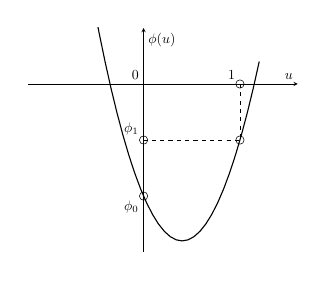
\begin{tikzpicture} [scale=0.5,c/.style={insert path={circle[radius=3pt]}}] 
\pgfplotsset{every axis/.append style={
		scale=1,
		axis lines=center,
		axis on top,
		xlabel={$u$},
		ylabel={$\phi(u)$},
               axis x line=middle,    % put the x axis in the middle
               axis y line=middle,    % put the y axis in the middle
               %x axis line style={-latex, ultra thin}, % arrows on the axis
               y axis line style={draw opacity=1},
                x axis line style={draw opacity=1},
            }}
     
					
	\tikzmath{\u=5;\a=4;\b=-2*\a;\d=-10;}
	 \u,\a, \b,\d;
    \pgfplotsset{ };
    
    \pgfplotsset{compat=1.12};
		\def\r{3};
		\def\H{1.0};  
		\def\s{0.123};
	\begin{axis}
		[
		xmin=-3,
		xmax=4,
		ymin=-15,
		ymax=5,
		xminorticks=true,
		yminorticks=false,
		ytick=\empty,
		xtick=\empty,
		]

		\addplot [black,thick,samples=40,samples y=0,	domain=-\r:\r,variable=\u]({\u},{\a*\u^2+\b*\u+\d});
		%\addplot [black,thick,samples=40,samples y=0,	domain=-\r:\r,variable=\u]({\u},{10*\a*\u^2+\b*\u+\d});

	\coordinate (x0) at ({0},{0});
	\coordinate (x1) at ({2.5},{0});
	\coordinate (p1) at ({2.5},{\a*2.5*2.5+\b*2.5+\d});
	\coordinate (p1y) at ({0},{\a*2.5*2.5+\b*2.5+\d});
	\coordinate (p1x) at ({2.5},{0});
	\coordinate (p2) at ({2.5},{10*\a+\b+\d});
	\coordinate (p2y) at ({0},{10*\a+\b+\d});
	\coordinate (p2x) at ({2.5},{0});
	\coordinate (p0) at ({0},{\d});
	\draw  (p0) [c];
	\draw  (p1) [c];
	\draw  (p1y) [c];
	\draw [dashed] (p1y)--(p1);
	\draw  (p1x) [c];
	\draw [dashed] (p1x)--(p1);
	\begin{comment}
	\draw  (p2) [c];
	\draw  (p2y) [c];
	\draw [dashed] (p2y)--(p2);
	\draw  (p2x) [c];
	\draw [dashed] (p2x)--(p2);
	\end{comment}
   	%\node[,{anchor=south east}] at (p1){$g_{0}$};
	\node[{anchor=north east}] at (p0){$\phi_0$};
	\node[{anchor=south east}] at (p1y){$\phi_1$};
	%\node[{anchor=south east}] at (p2x){$\phi_1$};
	\node[{anchor=south east }] at (x0){$0$};
	\node[{anchor=south east}] at (x1){$1$};
\end{axis}
\end{tikzpicture}
}
    \qquad
    \subfloat[]{            
\begin{tikzpicture} [scale=0.5,c/.style={insert path={circle[radius=3pt]}}] 
	\pgfplotsset{every axis/.append style={
		scale=1,
		axis lines=center,
		axis on top,
		xlabel={$u$},
		ylabel={$\phi(u)$},
               axis x line=middle,    % put the x axis in the middle
               axis y line=middle,    % put the y axis in the middle
               %x axis line style={-latex, ultra thin}, % arrows on the axis
               y axis line style={draw opacity=1},
                x axis line style={draw opacity=1},
            }}				
	\tikzmath{\u=5;\a=-1;\b=-4.15*\a;\d=-4;}
	 \u,\a, \b,\d;
    \pgfplotsset{ };
    
    \pgfplotsset{compat=1.12};
		\def\r{3};
		\def\H{1.0};  
		\def\s{0.123};
	\begin{axis}
		[
		xmin=-3,
		xmax=3,
		ymin=-10,
		ymax=5,
		xminorticks=true,
		yminorticks=false,
		ytick=\empty,
		xtick=\empty,
		]

		\addplot [black,thick,samples=40,samples y=0,	domain=-\r:\r,variable=\u]({\u},{\a*\u^2+\b*\u+\d});
		%\addplot [black,thick,samples=40,samples y=0,	domain=-\r:\r,variable=\u]({\u},{10*\a*\u^2+\b*\u+\d});

	\coordinate (x0) at ({0},{0});
	\coordinate (x1) at ({1},{0});
	\coordinate (p1) at ({1},{\a+\b+\d});
	\coordinate (p1y) at ({0},{\a+\b+\d});
	\coordinate (p1x) at ({1},{0});
	\coordinate (p2) at ({1},{10*\a+\b+\d});
	\coordinate (p2y) at ({0},{10*\a+\b+\d});
	\coordinate (p2x) at ({1},{0});
	\coordinate (p0) at ({0},{\d});
	\draw  (p0) [c];
	\draw  (p1) [c];
	\draw  (p1y) [c];
	\draw [dashed] (p1y)--(p1);
	\draw  (p1x) [c];
	\draw [dashed] (p1x)--(p1);
	\begin{comment}
	\draw  (p2) [c];
	\draw  (p2y) [c];
	\draw [dashed] (p2y)--(p2);
	\draw  (p2x) [c];
	\draw [dashed] (p2x)--(p2);
	\end{comment}
   	%\node[tdplot_main_coords,{anchor=south east}] at (p1){$g_{0}$};
	\node[{anchor=south east}] at (p0){$\phi_0$};
	\node[{anchor=north east}] at (p1y){$\phi_1$};
	%\node[tdplot_main_coords,{anchor=south east}] at (p2x){$\phi_1$};
	\node[{anchor=south east }] at (x0){$0$};
	\node[{anchor=south east}] at (x1){$1$};
\end{axis}
\end{tikzpicture}}
\caption{Non problematic null cone parametric functions.}
\label{fig:fig_p126_1a}
\end{figure}
\begin{figure}[H]%
    \centering
    \subfloat[]{               
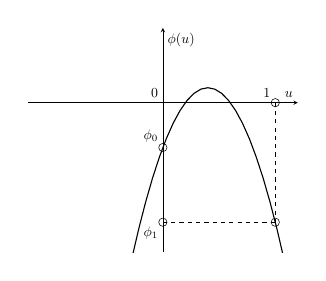
\begin{tikzpicture} [scale=0.5,c/.style={insert path={circle[radius=3pt]}}] 
\pgfplotsset{every axis/.append style={
		scale=1,
		axis lines=center,
		axis on top,
		xlabel={$u$},
		ylabel={$\phi(u)$},
               axis x line=middle,    % put the x axis in the middle
               axis y line=middle,    % put the y axis in the middle
               %x axis line style={-latex, ultra thin}, % arrows on the axis
               y axis line style={draw opacity=1},
                x axis line style={draw opacity=1},
            }}
					
	\tikzmath{\u=5;\a=-4;\b=-2*\a;\d=-3;}
	 \u,\a, \b,\d;
    \pgfplotsset{ };
    
    \pgfplotsset{compat=1.12};
		\def\r{3};
		\def\H{1.0};  
		\def\s{0.123};
	\begin{axis}
		[
		xmin=-3,
		xmax=3,
		ymin=-10,
		ymax=5,
		xminorticks=true,
		yminorticks=false,
		ytick=\empty,
		xtick=\empty,
		]

		\addplot [black,thick,samples=40,samples y=0,	domain=-\r:\r,variable=\u]({\u},{\a*\u^2+\b*\u+\d});
		%\addplot [black,thick,samples=40,samples y=0,	domain=-\r:\r,variable=\u]({\u},{10*\a*\u^2+\b*\u+\d});

	\coordinate (x0) at ({0},{0});
	\coordinate (x1) at ({2.5},{0});
	\coordinate (p1) at ({2.5},{\a*2.5*2.5+\b*2.5+\d});
	\coordinate (p1y) at ({0},{\a*2.5*2.5+\b*2.5+\d});
	\coordinate (p1x) at ({2.5},{0});
	\coordinate (p2) at ({2.5},{10*\a+\b+\d});
	\coordinate (p2y) at ({0},{10*\a+\b+\d});
	\coordinate (p2x) at ({2.5},{0});
	\coordinate (p0) at ({0},{\d});
	\draw  (p0) [c];
	\draw  (p1) [c];
	\draw  (p1y) [c];
	\draw [dashed] (p1y)--(p1);
	\draw  (p1x) [c];
	\draw [dashed] (p1x)--(p1);
	\begin{comment}
	\draw  (p2) [c];
	\draw  (p2y) [c];
	\draw [dashed] (p2y)--(p2);
	\draw  (p2x) [c];
	\draw [dashed] (p2x)--(p2);
	\end{comment}
   	%\node[tdplot_main_coords,{anchor=south east}] at (p1){$g_{0}$};
	\node[{anchor=south east}] at (p0){$\phi_0$};
	\node[{anchor=north east}] at (p1y){$\phi_1$};
	%\node[tdplot_main_coords,{anchor=south east}] at (p2x){$\phi_1$};
	\node[{anchor=south east }] at (x0){$0$};
	\node[{anchor=south east}] at (x1){$1$};
\end{axis}
\end{tikzpicture}}
\caption{Problematic null cone parametric functions.}
\label{fig:fig_p126_1b}
\end{figure}From the parabola's in figure $4.2.$ it is clear that the function can't reach $0$ in $u\in(0,1)$  and hence that the segment will not intersect the null cone.\\
One problematic could occur as represented in figure $4.3$.
For such a parabola, we have :
\begin{align}
\left\{\begin{array}{l} \ \ 
\phi(u)= au^2+bu+c\\\\
a = \left(\phi_1 +\phi_0-2\kappa\right) <0\\\\
b=2 \left(\kappa- \phi_0\right)\\\\
c=\phi_0\\\\
a+b=\phi_1-\phi_0\\\\
\phi_0<0\\\\
\phi_1 < 0
\end{array}\right.
\end{align}
From the $3$ known inequalities 
\begin{align}
\left\{\begin{array}{l} \ \ 
a < 0\\\\
\phi_0<0\\\\
\phi_1 < 0
\end{array}\right.
\end{align}
we get
\begin{align}
\left\{\begin{array}{l} \ \ 
a < 0\quad\Rightarrow\quad \kappa > \frac{\phi_1+\phi_0}{2} \\\\ b=2 \left(\kappa- \phi_0\right)\quad \Rightarrow\quad b > \phi_1-\phi_0\\\\
\end{array}\right.
\end{align}
Note that there is nothing special in the choice of $\phi_1, \ \phi_0$ as the segment is not oriented and as $\phi_1,\phi_0 <0$ we can put arbitrarily $b \geq0$ with $\phi_1 \geq \phi_0$.\\ 
Let's examine if there is a value $u_{max} \in (0,1)$ such that $\phi(u_{max})\geq 0$ and let us investigate whether the relation between the coefficients $a,b$ does not lead to a contradiction for such value of $u_{max} \in (0,1)$.  
\begin{align}
\dv{\phi(u)}{u}&=0\\
\Rightarrow\spatie u_{max} &= -\frac{b}{2a}\quad\text{ with } 0<b < -2a\\
\phi(u_{max}) &= -\frac{b^2}{4a}+\phi_0
\end{align}
Is it possible to have $\phi(u_{max}) \geq 0$ with $u_{max} \in (0,1)$? One straightforward condition to have this possible is that the discriminant of the quadratic equation os $b^2-4ac>=0$.
Hence,
\begin{align}
D &= \left[2 \left(\kappa- \phi_0\right)\right]^2-4\left(\phi_1 +\phi_0-2\kappa\right)\phi_0\\
&= 4\kappa^2+ 4\phi_0^2-8\kappa\phi_0-4\phi_1\phi_0 -4\phi_0^2+8\kappa\phi_0\\
&= 4\left(\kappa^2-\phi_1\phi_0\right)\\
&= \left\{\begin{array}{l} \ \ 
4\left[\left(y_1^{(0)}y_4^{(1)}-y_4^{(0)}y_1^{(1)}\right)^2
+\left(y_4^{(0)}y_2^{(1)}-y_2^{(0)}y_4^{(1)}\right)^2
+\left(y_4^{(0)}y_3^{(1)}-y_3^{(0)}y_4^{(1)}\right)^2\right]\\\\
-4\left[\left(y_2^{(0)}y_1^{(1)}-y_1^{(0)}y_2^{(1)}\right)^2
+\left(y_3^{(0)}y_1^{(1)}-y_1^{(0)}y_3^{(1)}\right)^2
+\left(y_3^{(0)}y_2^{(1)}-y_2^{(0)}y_3^{(1)}\right)^2\right]\\\\
\end{array}\right.
\end{align}
Obviously, this path of proving leads to nothing as $D$ can be positive even for a segment lying entirely in zone $I$ or $II$. To see that, take two events, stationary in  the space  at the point $P\left(0,0,y_3^{(0)}\right)$. The negative term in (39) disappears and obviously $D>0$.\\
$\dagger$WHAT IS THE ANALYTICAL WAY TO PROVE THIS? IS $a>0$ A CONDITION?$\dagger$
\end{comment}
\begin{comment}
\begin{figure}[H]
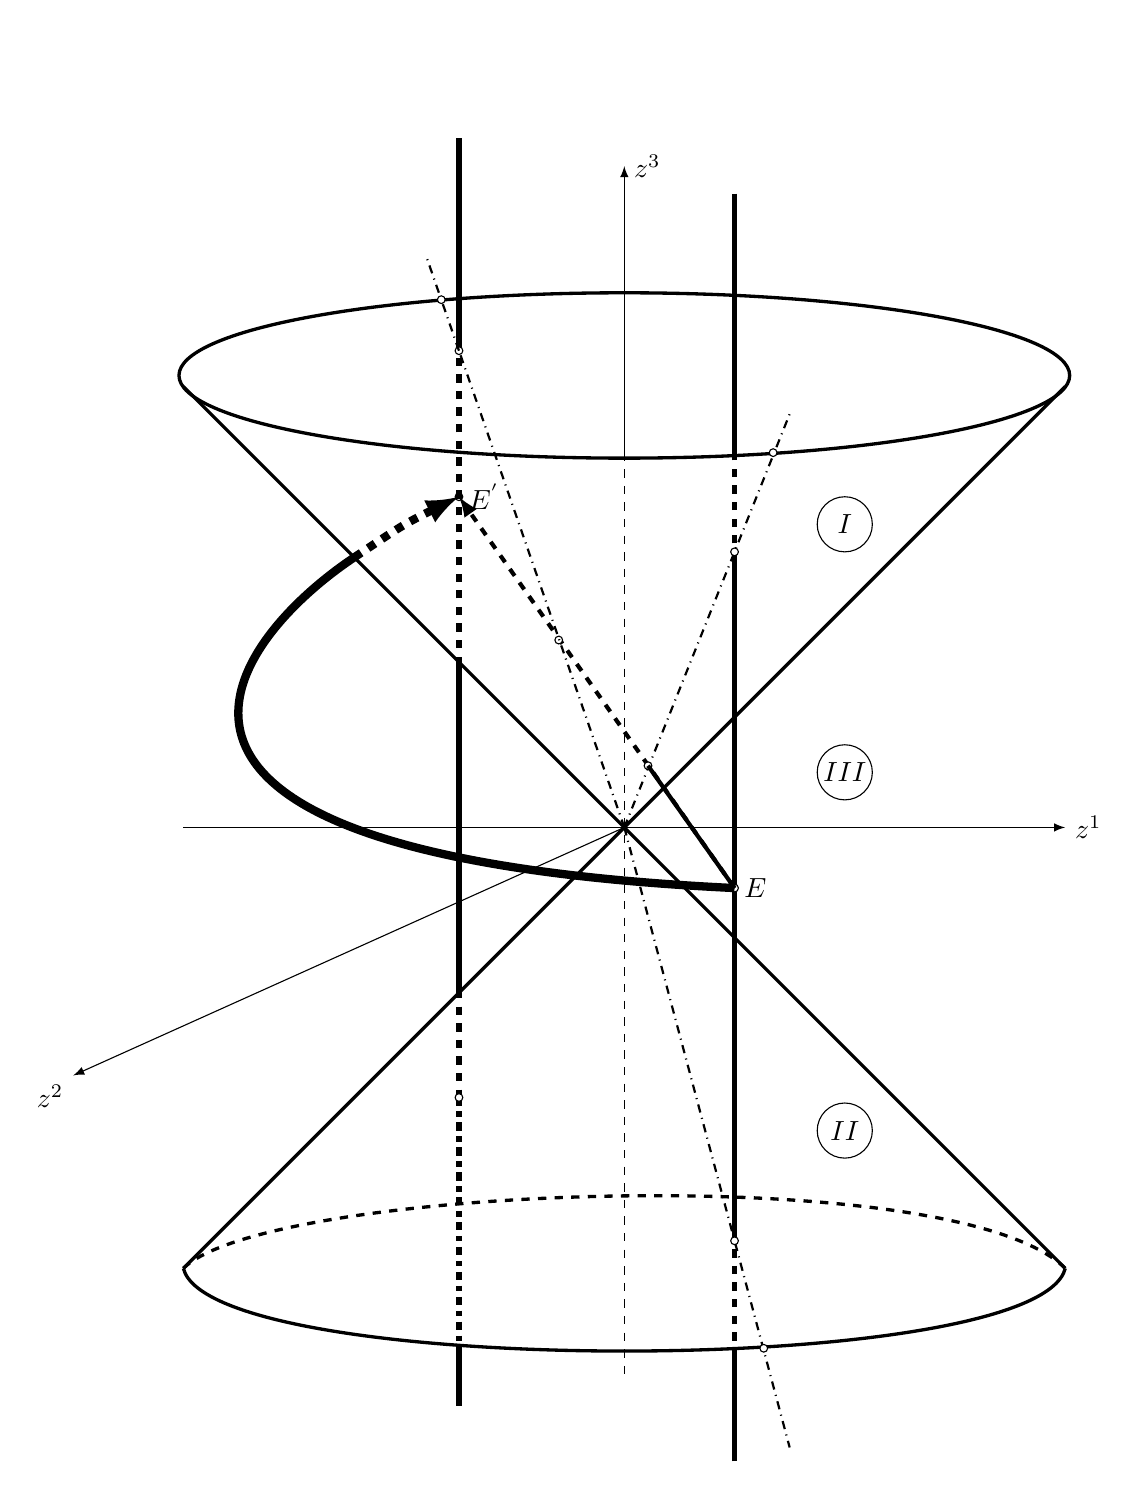
\begin{tikzpicture}[scale=0.70]
\coordinate (v1) at (-8,-0);
\coordinate (v2) at (8,-0) ;
\coordinate (v3) at (0,12) {};
\coordinate (v4) at (0,6.8) {};
\coordinate (v5) at (8,8) {};
\coordinate (v6)  at (0,0) {};
\coordinate (v7) at (-8,-8) {};
\coordinate (v8) at (8,-8) {};
\coordinate (v9) at (-8,8) {};
\coordinate (v10) at (-0,-10) {};
\coordinate (v11)  at (-10,-4.5) {};
\draw[-{latex}]  (v1)-- (v2)node[right] {$z^1$};
\draw  [-{latex}](v4)-- (v3)node[right] {$z^3$};
\draw  [-{latex}](v6)-- (v11)node[{anchor=north east}] {$z^2$};
\draw  [dashed](v4)-- (v10);
\draw[very thick]  (0,8.2) ellipse (8.08 and 1.5);
\draw [very thick] (v6) -- (v5);
\draw [very thick] (v7) -- (v6);
\draw  [very thick](v6) -- (v8);
\draw  [very thick](v6) -- (v9);
\draw[very thick] (-8,-8) .. controls (-7.5,-10) and (7.5,-10) .. (8,-8);
\draw [very thick, dashed,](-8,-8) .. controls (-6.5,-6.5) and (6,-6) .. (8,-8);

\coordinate (p0) at (-3.1,-1.4) {} {};
\coordinate (p1) at (2,-1.5) {} {};
\coordinate (p2) at (2,5) {} {};
\coordinate (p3) at (2,-7.5) {} {};
\coordinate (p4) at (5.5,0) {};

\draw [line width=2] (p2) -- (p1);
\draw [line width=2] (p2) -- (p3);
\coordinate (p5) at (2,6.7) {};
\coordinate (p6) at (2,-9.5) {};
\coordinate (p7)at (2,11.5) {};
\coordinate (p8)  at (2,-11.5) {};
\draw [dashed, line width=2] (p3) -- (p5);
\draw  [dashed, line width=2] (p2) -- (p6);
\draw [ line width=2] (p7) -- (p5);
\draw[ line width=2] (p8) -- (p6);

\coordinate (p9)  at (1.5*2,-1.5*7.5) {};
\coordinate (p10)  at (1.5*2,1.5*5) {};
\draw  [dashdotted,thick](v6) -- (p9);
\draw  [dashdotted,thick](v6) -- (p10);
\coordinate (t1) at (4,5.5) {};
\coordinate (t2) at (4,1) {} ;
\coordinate (t3) at (4,-5.5) {};
\draw[fill=black](t1)node[] {$I$};
\draw[fill=black](t2)node[] {$III$};
\draw[fill=black](t3)node[] {$II$};
\coordinate (t4) at (2.7,6.8) {};
\coordinate (t5) at (2.53,-9.45) {};
\draw[fill=white](t4) circle(2pt);
\draw[fill=white](t5) circle(2pt);

\draw  (t1) ellipse (0.5 and 0.5);
\draw  (t2) ellipse (0.5 and 0.5);
\draw  (t3) ellipse (0.5 and 0.5);
\draw  (-1.5,14.5) ellipse (0 and 0);
\coordinate (q1) at (2,-1.1) {} {} {};
\coordinate (q2) at (-3,6) {} {};
\draw[fill=white](q1) circle(2pt)node[{anchor=west }] {$E^{}$};
\draw[fill=white](q2) circle(2pt)node[{anchor=west }] {$E^{'}$};
\coordinate(q3) at (-4.9,4.9) {};
\draw [line width=3](q1) .. controls (-10.5,-0.5) and (-7,3.5) .. (q3);

\draw [line width=3,dashed, -latex](q3) .. controls (-4,5.5) and (-4,5.5) .. (q2);
\coordinate(s0) at (-3,12.5) {};
\coordinate(s1) at (-3,8.65) {};
\coordinate(s2) at (-3,-4.9) {};
\coordinate(s3) at (-3,2.95) {};
\coordinate(s4) at (-3,-2.95) {};
\coordinate(s5) at (-3,-9.5) {};
\coordinate(s6) at (-3,-10.5) {};
\coordinate(s7) at (-3*1.2,8.65*1.2) {};
\coordinate(s8) at (-3*1.107,8.65*1.107) {};
\draw [line width=2] (s1) -- (s0);
\draw [line width=2,dashed] (s3) -- (s1);
\draw [line width=2] (s3) -- (s4);
\draw [line width=2,dashdotted] (s2) -- (s5);
\draw [line width=2,dashed] (s4) -- (s2);
\draw [line width=2] (s5) -- (s6);
\draw[fill=white](s1) circle(2pt);
\draw[fill=white](s2) circle(2pt);
\draw[fill=white](p3) circle(2pt);
\draw[fill=white](p2) circle(2pt);
\draw [line width=1.5, dashed,-latex] (q1) -- (q2);
\coordinate(w0) at (-1*1.19,3.4) {} {};
\coordinate(w1)  at (0.43,1.12) {};
\draw[fill=white](w0) circle(2pt);
\draw[fill=white](w1) circle(2pt);
\draw  [dashdotted,thick](v6) -- (s1);
\draw  [dashdotted,thick](s1) -- (s7);
\draw[fill=white](s8) circle(2pt);
\draw [line width=1.5, ] (w1) -- (q1);
\end{tikzpicture}
\caption{Travelling between two points in region III (present) in a  $V_3$ space-time manifold}
\label{fig:fig_p96_3415_b}
\end{figure}
\end{comment}
$$\dagger$$
$$\blacklozenge$$
\newpage

\section{p133 - Exercise}
\begin{tcolorbox}
In a space of two dimensions prove the relation
$$\mathbf{4.318.}\spatie \epsilon_{mp}\epsilon_{mq} = \delta_{pq}$$
\end{tcolorbox}
Suppose $p=q$, then in the summation the term is $0$ if $m=p=q$ and the remaining term is $1\times 1$ or $-1\times -1$ giving indeed $\delta_{pq}=1$.\\ 
If  $p\neq q$ we get either $m=p$ or $m=q$ in each term of the summation and hence all terms vanish.
$$\blacklozenge$$
\newpage

\section{p135 - Clarification}
\begin{tcolorbox}
$$\mathbf{4.324.}\spatie P_{mn}= \epsilon_{mnrs}X_rY_s$$
In 4.323 a skew-symmetric tensor is formed.
\end{tcolorbox}
Let's check whether $P_{mn}$ is indeed a tensor and if it is an oriented one.
Be an orthogonal transformation (proper or not)
\begin{align}
X^{'}_r = A_{rm}X_m+A_r
\end{align}
and let's check how the expression $P^{'}_{mn}= P_{rs}\partial_m X_r \partial_n X_s$ behaves.

\begin{align}
P^{'}_{mn}&= P_{rs}\partial_m z_r \partial_n z_s\\
\mathbf{(4.303.)\ }\Rightarrow \spatie &= \epsilon_{rspq}X_pY_q A_{mr}A_{ns}
\end{align}
From (4.302.) we have
\begin{align}
X_p = A_{kp}X^{'}_k -  A_{kp}A_k
\end{align}
Replacing this in (3)
\begin{align}
P^{'}_{mn}&=  \epsilon_{rspq}\left(A_{kp}X^{'}_k -  A_{kp}A_k\right)\left(A_{tq}Y^{'}_t -  A_{tq}A_t\right) A_{mr}A_{ns}\\
&=\left\{\begin{array}{l}
\epsilon_{rspq}A_{mr}A_{ns}A_{kp}A_{tq}X^{'}_kY^{'}_t \\\\
-\epsilon_{rspq}A_{mr}A_{ns}A_{kp}A_{tq}X^{'}_kA_t \\\\
-\epsilon_{rspq}A_{mr}A_{ns}A_{kp}A_{tq}Y^{'}_tA_k \\\\
+\epsilon_{rspq}A_{mr}A_{ns}A_{kp}A_{tq}A_kA_t 
\end{array}\right.\\
&= \epsilon_{rspq}A_{mr}A_{ns}A_{kp}A_{tq}\left(X^{'}_k-A_k\right)\left(Y^{'}_t-A_t\right)
\end{align}
A analogous reasoning as in (4.316.) gives us $\epsilon_{mnkt}\left|A_{mr}\right|=\epsilon_{rspq}A_{mr}A_{ns}A_{kp}A_{tq}$ and so 
\begin{align}
P^{'}_{mn}&= \epsilon_{mnkt}\left|A_{mr}\right| \left(X^{'}_k-A_k\right)\left(Y^{'}_t-A_t\right)
\end{align}
Apparently, even with $\left|A_{mr}\right| =1$ , $P_{mn}$ does not behave like a tensor due to the $ \left(X^{'}_k-A_k\right)\left(Y^{'}_t-A_t\right)$ components. But of course, this is consequence of the sloppy use of the transformation equation: equation (1) is the transformation rule for a point in the $V_4$ space but the object $P_{mn}$ takes two vectors as input. If we consider a vector as an object defined by an ordered pair i.e. $X\equiv \left(z^{(1)}_{(X)}, z^{(0)}_{(X)}\right)$ then $P_{mn}$ should be defined as $P_{mn}= \epsilon_{mnrs}\left(z^{(1)}_{(X)r}- z^{(0)}_{(X)r}\right)\left(z^{(1)}_{(Y)s}- z^{(0)}_{(Y)s}\right)$. This means that when using the transformation rule (1) we will get $$X^{'}\equiv \left(z^{'(1)}_{(X)}, z^{'(0)}_{(X)}\right)$$ giving as components 
\begin{align}X^{'}_r &= z^{'(1)}_{(X)r}- z^{'(0)}_{(X)r}\\&=   A_{rm}z^{(1)}_{(X)m}+A_r-A_{rm}z^{(0)}_{(X)m}-A_r\\
&= A_{rm}\left(z^{(1)}_{(X)m} -z^{(0)}_{(X)m}\right)
\end{align}
Replacing all this we get as a more correct representation of $p_{mn}$ and $P^{'}_{mn}$:
\begin{align}
\left\{\begin{array}{l}
P_{mn}= \epsilon_{mnrs}\left(z^{(1)}_{(X)r}- z^{(0)}_{(X)r}\right)\left(z^{(1)}_{(Y)s}- z^{(0)}_{(Y)s}\right)\\\\
P^{'}_{mn}= \epsilon_{mnkt}\left|A_{mr}\right| \left(z^{'(1)}_{(X)r}- z^{'(0)}_{(X)r}\right)\left(z^{'(1)}_{(Y)s}- z^{'(0)}_{(Y)s}\right)\\\\
\end{array}\right.
\end{align}
We see that indeed $P_{mn}$ is an oriented Cartesian tensor.
$$\blacklozenge$$
\newpage

\section{p135 - Exercise}
\begin{tcolorbox}
Write out the six independent non-zero components of $P_{mn}$ as given by $\mathbf{4.324.}$
\end{tcolorbox}
We have 
\begin{align}
\mathbf{4.324.}\spatie P_{mn}= \in_{mnrs}X^rY^s\\
\text{with}\quad \spatie m=n \quad \Rightarrow \quad P_{mn}= 0
\end{align}
So, the six independent components are in the set $\{mn\}= \left\{12,13,14,23,24,34 \right\}$ as $P_{nm}=-P_{mn}$.
\begin{align}
&\left\{\begin{array}{l}\\
P_{12} = \in_{1234}X^3Y^4+\in_{1243}X^4Y^3\\\\
P_{13} = \in_{1324}X^2Y^4+\in_{1342}X^4Y^2\\\\
P_{14} = \in_{1423}X^2Y^3+\in_{1432}X^3Y^2\\\\
P_{23} = \in_{2314}X^1Y^4+\in_{2341}X^4Y^1\\\\
P_{24} = \in_{2413}X^1Y^3+\in_{2431}X^3Y^1\\\\
P_{34} = \in_{3412}X^1Y^2+\in_{3421}X^2Y^1\\\\
\end{array}\right.\\
&\left\{\begin{array}{l}\\
P_{12} = X^3Y^4-X^4Y^3\\\\
P_{13} = -X^2Y^4+X^4Y^2\\\\
P_{14} = X^2Y^3-X^3Y^2\\\\
P_{23} = X^1Y^4-X^4Y^1\\\\
P_{24} = -X^1Y^3+X^3Y^1\\\\
P_{34} = X^1Y^2-X^2Y^1\\\\
\end{array}\right.
\end {align}
$$\blacklozenge$$
\newpage

\section{p136 - Exercise}
\begin{tcolorbox}
Translate the well-known vector relations
$$A\times (B\times C)= B(A.  C)-C(A.B)$$
$$\nabla \times (\nabla \times V)= \nabla (\nabla .  V )-\nabla^2V$$
into Cartesian tesnor form, and prove the by use of $4.329$.
\end{tcolorbox}
We have 
\begin{align}
\mathbf{4.329.}\spatie \in_{mrs}\in_{mpq} = \delta_{rp}\delta_{sq}-\delta_{rq}\delta_{sp}
\end{align}
The first identity
\begin{align}
A\times (B\times C)= B(A.  C)-C(A.B)\\
\Leftrightarrow\spatie \in_{npm}\in_{mrs}A_p B_r C_s = A_p\left(B_n C_p-C_n B_p\right)
\end{align}
Indeed,
\begin{align}
(B\times C)_m &= \in_{mrs}B_rC_s\\
\Rightarrow\spatie \left(A\times (B\times C)\right)_n &=\in_{npm}A_p \in_{mrs}B_rC_s\\
&=-\in_{mpn}\in_{mrs}A_p \in_{mrs}B_r C_s\\
&= -\delta_{pr}\delta_{ns}A_pB_rC_s+\delta_{ps}\delta_{nr}A_pB_rC_s\\
&= A_pB_nC_p-A_pB_pC_n\\
\Leftrightarrow\spatie & B(A.  C)-C(A.B)
\end{align}
The second identity
\begin{align}
\nabla \times (\nabla \times V)&= \nabla (\nabla .  V )-\nabla^2V\\
\Leftrightarrow \spatie \in_{nrm}\in_{mpq}V_{q,pr} &= V_{p,pn}- V_{n,pp}
\end{align}
Indeed,
\begin{align}
\left(\nabla \times V\right)_m &= \in_{mpq}V_{q,p}\\
\Rightarrow\spatie \left(\nabla  \times (\nabla \times V)\right)_n &=\in_{nrm}\left(\in_{mpq}V_{q,p}\right)_{,r}\\
 &=\in_{nrm}\in_{mpq}V_{q,pr}\\
 &=\delta_{rq}\delta_{np}V_{q,pr}-\delta_{pr}\delta_{nq}V_{q,pr}\\
 &= V_{p,pn}-V_{n,pp}
\end{align}
We have also
\begin{align}
\left(\nabla V\right) &= V_{p,p}\\
\Rightarrow\spatie \left(\nabla (\nabla .  V )\right)_n &= \left(V_{p,p}\right)_n\\
&= V_{p,pn}
\end{align}
and 
\begin{align}
\nabla^2 V_n  & \equiv  V_{n,pp} \\
\Rightarrow\spatie \left(\nabla (\nabla .  V )\right)_n- \nabla^2 V_n &= V_{p,pn}- V_{n,pp}
\end{align}
which corresponds to (15).
So the tensor expression in Cartesian tensor form can be written as 
$$\in_{nrm}\in_{mpq}V_{q,pr} = V_{p,pn}- V_{n,pp}$$

$$\blacklozenge$$
\newpage

\section{p139 - Exercise 1.}
\begin{tcolorbox}
Show that, in a 3-space of constant curvature $-\frac{1}{R^2}$ and positive definite metric form, the line element in polar coordinate is 
$$ds^2= dr^2+R^2\sinh^2\left(\frac{r}{R}\right)\left(d\theta^2+\sin^2\theta d\phi^2\right)$$
\end{tcolorbox}
We have by $4.120c$
\begin{align}
X_r \eta^r &= A\sinh \left(s\sqrt{-\epsilon K}\right)
\end{align}
We choose $N$ different $X^{(k)}_r$ $(k= 1,2,\dots, N)$ which are orthonormal.
Applying $(1)$ $N$ times with the different $X^{(k)}_r$ $(k= 1,2,\dots, N)$, we get
\begin{align}
X^{(k)}_r \eta^r &= A^{(k)}\sinh \left(s\sqrt{-\epsilon K}\right)
\end{align}
But as the $X^{(k)}_r$ are orthonormal and are used as a basis at the considered point of the geodesic we have 
\begin{align}
X^{(k)}_r &= \delta^k_r
\end{align}
So, $(2)$ becomes
\begin{align}
\eta^k &= A^{(k)}\sinh \left(s\sqrt{-\epsilon K}\right)
\end{align}
which are the components of the displacement vector in the orthonormal basis. By $\mathbf{2.301.}$ :
\begin{align}
Y^2 &= \epsilon a_{mn} Y^m Y^n\\
\Rightarrow \spatie \eta^2 &= \epsilon a_{mn} A^{(m)} A^{(n)}\sinh^2 \left(s\sqrt{-\epsilon K}\right)\\
\Rightarrow \spatie \eta &= C\left|\sinh \left(s\sqrt{-\epsilon K}\right)\right|\\
\text{with}\spatie C&= \sqrt{\left|\epsilon a_{mn} A^{(m)} A^{(n)}\right|}
\end{align}
As $\epsilon =1$ (positive-definite metric) and $K=-\frac{1}{R^2}$
we have
\begin{align}
\eta &= C\left|\sinh \left(\frac{s}{R}\right)\right|
\end{align}
From this and using the very same reasoning from $4.126.$ to $4.130.$ (pages 117-119) we get 
$$ds^2= dr^2+R^2\sinh^2\left(\frac{r}{R}\right)\left(d\theta^2+\sin^2\theta d\phi^2\right)$$
$$\blacklozenge$$
\newpage


\section{p139 - Exercise 2.}
\begin{tcolorbox}
Show that the volume of an antipodal 3-space of positive-definite metric form and positive constant curvature $\frac{1}{R^2}$ is $2\pi^2R^3$. (Use the equation 4.130. to find the area of a sphere $r= \text{constant}$ in polar coordinates. Multiply by $dr$ and integrate for $0\leq r \leq \pi R$ to get the volume). What is the volume if the space is polar?
\end{tcolorbox}
We have  $4.130$
\begin{align}
ds^2= dr^2+R^2\sin^2\left(\frac{r}{R}\right)\left(d\theta^2+\sin^2\theta d\phi^2\right)
\end{align}
Having a positive-definite metric form, the space can be locally considered as Euclidean and an elementary area of a  surface with constant $r (\rightarrow dr=0)$ can be calculated as $dS=ds_{d\theta=0}ds_{d\phi=0}$ and get by (1)
\begin{align}
dS &= R^2\sin^2\left(\frac{r}{R}\right)\sin\theta d\phi d\theta\\
\Rightarrow\spatie\frac{S}{8} &= R^2\sin^2\left(\frac{r}{R}\right)\int^{\frac{\pi}{2}}_{0}\int^{\frac{\pi}{2}}_{0} \sin\theta d\phi d\theta\\ 
&= R^2\sin^2\left(\frac{r}{R}\right)\frac{\pi}{2} \left.\left(-\cos\theta \right)\right|^{\frac{\pi}{2}}_{0}\\
\Rightarrow\spatie S&= 4\pi R^2\sin^2\left(\frac{r}{R}\right)
\end{align}
We see that the area is a cyclic function of $r$ having zeros' at $r= k\frac{\pi}{R }, k=1,2,\dots$
\begin{figure}[H]
\begin{center}
\begin{tikzpicture}[]
    \begin{axis}[
    domain = 0:2.5*pi,
    samples = 201,
    axis on top = true,
    grid =none,
    grid style = {dashed, line width=.1pt, draw=gray!30, 
    /pgfplots/on layer=axis background},
    		ytick=\empty,
		xtick=\empty,
		xmin=-0,
		xmax=9,
		ymin=0,
		ymax=1.5,
]
\addplot+[no marks, color=black] {(sin(deg(x)))^2};
\node[{anchor=south east}] at (0,10){$\phi_0$};
\end{axis}
\coordinate(0) at (0,0);
\node[{anchor=north east }] at (0){$0$};
\coordinate(p1) at (2.7,0);
\node[{anchor=north east }] at (p1){$\pi$};
\coordinate(p2) at (2*2.5,0);
\node[{anchor=north east }] at (p2){$2\pi$};
\end{tikzpicture}
\caption{Area of an antipodal 3-space of positive-definite metric form}
\label{fig:fig_p138_Ex2}
\end{center}
\end{figure}
So, there are good reasons to restrict $r$ to $[0,\pi R]$ as otherwise all space of that type would have infinite volume, whatever it's curvature. So, we get as volume 
\begin{align}
V &= 4\pi R^2\int^{\pi R}_{0}\sin^2\left(\frac{r}{R}\right)dr\\
&= 4\pi R^3\int^{\pi R}_0\sin^2\left(\frac{r}{R}\right)d\left(\frac{r}{R}\right)\\
&= 4\pi R^3\left.\left( \half x - \frac{1}{4}\sin2x \right)\right|^{\pi}_0\\
&= 2\pi^2 R^3
\end{align}
For a polar space, the volume would be half of that of an antipodal one (with same curvature of course) as in (3) we would consider only 4 quadrants instead of 8.
$$\blacklozenge$$
\newpage


\section{p139 - Exercise 3.}
\begin{tcolorbox}
By direct calculation of the tensor $R_{rsmn}$ verify that $\mathbf{4.130.}$ is the metric form of a space of constant curvature.
\end{tcolorbox}
We have  $4.130$
\begin{align}
ds^2&= dr^2+R^2\sin^2\left(\frac{r}{R}\right)\left(d\theta^2+\sin^2\theta d\phi^2\right)\\
\Rightarrow\spatie &
\ (a_{mn}) = \begin{pmatrix}
 1& 0 & 0\\
0 & R^2\sin^2\left(\frac{r}{R}\right) & 0 \\
0 & 0 & R^2\sin^2\left(\frac{r}{R}\right)\sin^2\theta \\
\end{pmatrix}
\end{align}
Now for $R_{rsmn}$ we refer to exercise 7 page 109 of chapter 3, where the curvature tensor was calculated for a general case of the form 
$$ ds^2= (h_1dx^1)^2+(h_2dx^2)^2+(h_3dx^3)^2$$ where $h_1, h_2, h_3$ are functions of the three coordinates.
We have then for our case
\begin{align}
\left\{\begin{array}{l}
h_1 = 1\\\\
h_2 = R\sin\left(\frac{r}{R}\right)\\\\
h_3 = R\sin\left(\frac{r}{R}\right)\sin\theta\\\\
\end{array}\right.
\end{align}
In the exercise we got for the non-vanishing curvature tensors
\begin{align}
R_{1212}&=
-h_2\partial_{11}^2(h_2)-h_1\partial_{22}^2(h_1)
+\frac{h_2}{h_1}\partial_1 h_1\partial_1 h_2+\frac{h_1}{h_2}\partial_2 h_1\partial_2 h_2-\frac{h_1 h_2}{h_3^2}\partial_3 h_1\partial_3 h_2\\
R_{2323}&=
-h_3\partial_{22}^2(h_3)-h_2\partial_{33}^2(h_2)
+\frac{h_3}{h_2}\partial_2 h_2\partial_2 h_3+\frac{h_2}{h_3}\partial_3 h_2\partial_3 h_3-\frac{h_2 h_3}{h_1^2}\partial_1 h_2\partial_1 h_3\\
R_{1313}&=
-h_3\partial_{11}^2(h_3)-h_1\partial_{33}^2(h_1)
+\frac{h_3}{h_1}\partial_1 h_1\partial_1 h_3+\frac{h_1}{h_3}\partial_3 h_1\partial_3 h_3-\frac{h_1 h_3}{h_2^2}\partial_2 h_1\partial_2 h_3
\end{align}
\begin{align}
R_{1213}&=-h_1\partial_{32}^2(h_1)+\frac{h_1}{h_3}\partial_2 h_3\partial_3 h_1+\frac{h_1}{h_2}\partial_2 h_1\partial_3 h_2\\
R_{1223}&=h_2\partial_{31}^2(h_2)-\frac{h_2}{h_1}\partial_1 h_2\partial_3 h_1-\frac{h_2}{h_3}\partial_3 h_2\partial_1 h_3\\
R_{1323}&=
-h_3\partial_{21}^2(h_3)+\frac{h_3}{h_1}\partial_1 h_3\partial_3 h_1+\frac{h_3}{h_2}\partial_2 h_3\partial_1 h_2
\end{align}
Clearly $\partial_{k}^2(h_1)=0$ and $\partial_{mn}^2(h_1)=0$ and considering $h_2 = h_2(r), \ h_3 = h_3(r,\theta)$
we can simplify 
\begin{align}
R_{1212}&=
-h_2\partial_{11}^2(h_2)\\
R_{2323}&=
-h_3\partial_{22}^2(h_3)
-\frac{h_2 h_3}{h_1^2}\partial_1 h_2\partial_1 h_3\\
R_{1313}&=
-h_3\partial_{11}^2(h_3)
\end{align}
\begin{align}
R_{1213}&=0\\
R_{1223}&=0\\
R_{1323}&=
-h_3\partial_{21}^2(h_3)+\frac{h_3}{h_2}\partial_2 h_3\partial_1 h_2
\end{align}
with 
\begin{align}
\left\{\begin{array}{l}
\partial_1 h_2=\cos\left(\frac{r}{R}\right)\\\\
\partial_1 h_3=\cos\left(\frac{r}{R}\right)\sin\theta\\\\
\partial_2 h_3=R\sin\left(\frac{r}{R}\right)\cos\theta\\\\
\partial^2_{11} h_2=-\frac{1}{R}\sin\left(\frac{r}{R}\right)\\\\
\partial^2_{11} h_3=-\frac{1}{R}\sin\left(\frac{r}{R}\right)\sin\theta\\\\
\partial^2_{21} h_3=\cos\left(\frac{r}{R}\right)\cos\theta\\\\
\partial^2_{22} h_3=-R\sin\left(\frac{r}{R}\right)\sin\theta\\\\
\end{array}\right.
\end{align}
giving
\begin{align}
R_{1212}&=
\sin^2\left(\frac{r}{R}\right)\\
R_{2323}&=
R^2\sin^2\left(\frac{r}{R}\right)\sin^2\theta 
-R^2\sin^2\left(\frac{r}{R}\right)\sin^2\theta\cos^2\left(\frac{r}{R}\right)\\
&= R^2\sin^4\left(\frac{r}{R}\right)\sin^2\theta\\
R_{1313}&=\sin^2\left(\frac{r}{R}\right)\sin^2\theta\\
R_{1213}&=0\\
R_{1223}&=0\\
R_{1323}&=
-R\sin\left(\frac{r}{R}\right)\sin\theta\cos\left(\frac{r}{R}\right)\cos\theta+\sin\theta R\sin\left(\frac{r}{R}\right)\cos\theta\cos\left(\frac{r}{R}\right)\\&=0
\end{align}
and considering the symmetries
\begin{align}
R_{1212}&=-R_{1221}=-R_{2112}=
\sin^2\left(\frac{r}{R}\right)\\
R_{2323}&=-R_{2332}=-R_{3223}= R^2\sin^4\left(\frac{r}{R}\right)\sin^2\theta\\
R_{1313}&=-R_{1331}=-R_{3113}=\sin^2\left(\frac{r}{R}\right)\sin^2\theta\\
\end{align}
By $\mathbf{4.114.}$
\begin{align}
R_{rsmn}&= K\left(a_{rm}a_{sn}-a_{rn}a_{sm}\right)\\
\Rightarrow\spatie &\left\{\begin{array}{l}
R_{1212}= K\left(a_{11}a_{22}-a_{12}a_{21}\right)\\
R_{2323}= K\left(a_{22}a_{33}-a_{23}a_{32}\right)\\
R_{1313}= K\left(a_{11}a_{33}-a_{13}a_{31}\right)
\end{array}\right.\\
\Rightarrow\spatie &\left\{\begin{array}{l}
R_{1212}= K R^2\sin^2\left(\frac{r}{R}\right)\\
R_{2323}= K R^2\sin^2\left(\frac{r}{R}\right)R^2\sin^2\left(\frac{r}{R}\right)\sin^2\theta\\
R_{1313}= K R^2\sin^2\left(\frac{r}{R}\right)\sin^2\theta\\
\end{array}\right.\\
\Rightarrow\spatie &\left\{\begin{array}{l}
R_{1212}= K R^2\sin^2\left(\frac{r}{R}\right)\\
R_{2323}= K R^4\sin^4\left(\frac{r}{R}\right)\sin^2\theta\\
R_{1313}= K R^2\sin^2\left(\frac{r}{R}\right)\sin^2\theta\\
\end{array}\right.
\end{align}
 replacing (25), (26) and (27) in (32) we get
 \begin{align}
\left\{\begin{array}{l}
\sin^2\left(\frac{r}{R}\right)= K R^2\sin^2\left(\frac{r}{R}\right)\\
R^2\sin^4\left(\frac{r}{R}\right)\sin^2\theta= K R^4\sin^4\left(\frac{r}{R}\right)\sin^2\theta\\
\sin^2\left(\frac{r}{R}\right)\sin^2\theta= K R^2\sin^2\left(\frac{r}{R}\right)\sin^2\theta\\
\end{array}\right.
\end{align}
giving indeed for the three curvature tensors $K=\frac{1}{R^2}$\\
With this, the question of the  exercise is answered but we go a little bit further and investigate for this practical case the equations of $\mathbf{4.115.}$ and  calculate $R=a^{mn}R_{mn}$. With $R$, the curvature invariant. To avoid confusion with the curvature $R$ itself we use $\mathfrak{R}$ for the curvature invariant.\\
As the metric tensor is diagonal:

\begin{align}
\mathfrak{R}=a^{11}R_{11}+a^{22}R_{22}+a^{33}R_{33}\\
\end{align}
and 
\begin{align}
R_{mn}&= a^{sn}R_{srmn}\\
\Rightarrow\spatie &
\left\{\begin{array}{l}
R_{11} = a^{11}R_{1111}+a^{22}R_{2112}+a^{33}R_{3113}\\\\
R_{22} = a^{11}R_{1221}+a^{22}R_{2222}+a^{33}R_{3223}\\\\
R_{33} = a^{11}R_{1331}+a^{22}R_{2332}+a^{33}R_{3333}\\\\
\end{array}\right.\\
\Rightarrow\spatie &\left\{\begin{array}{l}
R_{11} = -a^{22}\sin^2\left(\frac{r}{R}\right)-a^{33}\sin^2\left(\frac{r}{R}\right)\sin^2\theta\\\\
R_{22} = -a^{11}\sin^2\left(\frac{r}{R}\right)-a^{33}R^2\sin^4\left(\frac{r}{R}\right)\sin^2\theta\\\\
R_{33} = -a^{11}\sin^2\left(\frac{r}{R}\right)\sin^2\theta-a^{22}R^2\sin^4\left(\frac{r}{R}\right)\sin^2\theta\\\\
\end{array}\right.\\
\Rightarrow\spatie &\left\{\begin{array}{l}
R_{11} = -\frac{\sin^2\left(\frac{r}{R}\right)}{R^2\sin^2\left(\frac{r}{R}\right)}-\frac{\sin^2\left(\frac{r}{R}\right)\sin^2\theta}{R^2\sin^2\left(\frac{r}{R}\right)\sin^2\theta}\\\\
R_{22} = -\sin^2\left(\frac{r}{R}\right)-\frac{R^2\sin^4\left(\frac{r}{R}\right)\sin^2\theta}{R^2\sin^2\left(\frac{r}{R}\right)\sin^2\theta}\\\\
R_{33} = -\sin^2\left(\frac{r}{R}\right)\sin^2\theta-\frac{R^2\sin^4\left(\frac{r}{R}\right)\sin^2\theta}{R^2\sin^2\left(\frac{r}{R}\right)}\\\\
\end{array}\right.
\end{align}
giving
\begin{align}
\left\{\begin{array}{l}
R_{11} = -\frac{2}{R^2}\\\\
R_{22} = -2\sin^2\left(\frac{r}{R}\right)\\\\
R_{33} = -2\sin^2\left(\frac{r}{R}\right)\sin^2\theta\\\\
\end{array}\right.
\end{align}
hence
\begin{align}
\mathfrak{R}&=a^{11}R_{11}+a^{22}R_{22}+a^{33}R_{33}\\
\Rightarrow\spatie \mathfrak{R}&= -\frac{2}{R^2}-2\frac{\sin^2\left(\frac{r}{R}\right)}{R^2\sin^2\left(\frac{r}{R}\right)}-2\frac{\sin^2\left(\frac{r}{R}\right)\sin^2\theta}{R^2\sin^2\left(\frac{r}{R}\right)\sin^2\theta }\\
&= -\frac{6}{R^2}
\end{align}
The equations in (40) and (43) are indeed in accordance with $\mathbf{4.115}$ .
$$\blacklozenge$$
\newpage

\section{p139 - Exercise 4}
\begin{tcolorbox}
Show that if $V_N$ has positive-definite metric form and constant positive curvature $K$, then coordinates $y^r$ exist so that
$$ds^2=\frac{dy^m dy^m}{\left(1+\kwart y^n y^n\right)^2}$$
(Starting with a coordinate system $x^r$ which is locally Cartesian at $O$, take at any point $P$ the coordinates
$$y^r=p^r\frac{2}{\sqrt{K}}\tan\left(\half r \sqrt{K}\right)$$
where $p^r$ ar the the components of the unit tangent vector $\left(\dv{x^r}{s}\right)$ at $O$ to the geodesic $OP$ and $r$ is the geodesic distance $OP$.)
\end{tcolorbox}
Let us first understand what happens. Fig.1.5 for a $V_3$ will help us understand.
Let $P$ and $P+dP$ be two points separated by an infinitesimal distance. Consider the two geodesics initiated from the origin and joining these two points. Be $X$ and $X^{'}$ the two tangents unit vectors  to these geodesics. Those vectors have components $p^r=\dv{x^r}{s}$ taken along their respective geodesics.  By the considered mapping, $y^r=p^r\frac{2}{\sqrt{K}}\tan\left(\half r \sqrt{K}\right)$, the points $P$ and $P+dP$ are mapped on the  points  $\tau (P)$ and $\tau (P+dP)$ with $\left|O\tau (P)\right|$ and $\left|O\tau (P+dP)\right|$ collinear with the  two tangents unit vectors  $X$ and $X^{'}$ . \\
Observe also the segment $PN$ which corresponds to the geodesic displacement $\eta$ for the geodesic distance $r=OP$. As the metric form is positive-definite, we can consider that the infinitesimal triangle $\left|\widehat{PNP+dP}\right|$ lies in an infinitesimally Euclidean space and  we can express $ds^2=\eta^2+ dr^2$ as $\left|NP+dP\right| = dr$. Observe now, the triangle $\left|\widehat{\tau(P)\tau(N)\tau(P+dP)}\right|$. There also we have $\left|\tau(P+dP)\tau(P)\right|^2 = \left|\tau(P)\tau(N)\right|^2+\left|\tau(P+dP)\tau(N)\right|^2$. Can we find a relationship between these two triangle?\\
\begin{figure}[H]
\begin{center}
\usetikzlibrary {arrows.meta}
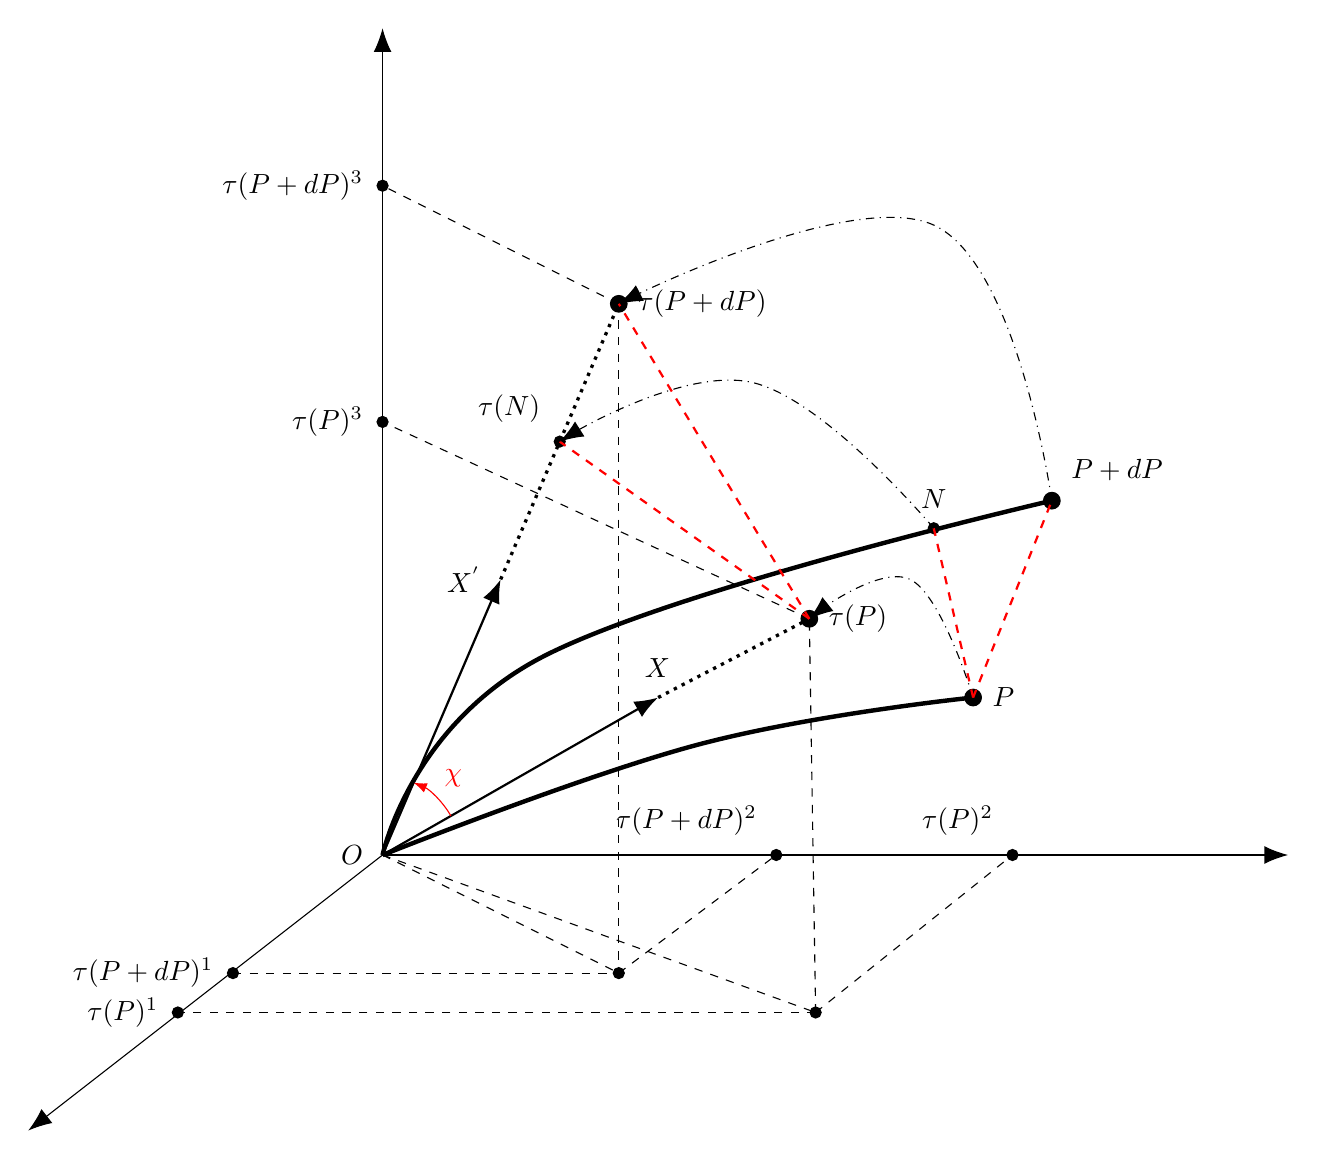
\begin{tikzpicture}

\coordinate (v1) at (-0.5,0) {};
\coordinate  (v2) at (-0.5,10.5) {} {};
\coordinate  (v4) at (-5,-3.5) {};
\coordinate  (v3) at (11,0) {};
\draw [-{Latex[length=3mm]}] (v1) -- (v2);
\draw  [-{Latex[length=3mm]}] (v1)-- (v3);
\draw   [-{Latex[length=3mm]}](v1) -- (v4);

\coordinate  (c1) at (7,2) {};
\coordinate  (c2) at (8,4.5) {};
\draw[ultra thick]  plot[,smooth, tension=.7] coordinates {(v1) (3.5,1.4) (c1)};
\draw [ultra thick]  plot[smooth, tension=.7] coordinates {(v1) (1.5,2.5) (c2)};

\coordinate  (v5) at (1,3.5) {};
\coordinate  (v5b) at (2*1.25,2*3.5) {};
\draw  [dotted, very thick](v5) -- (v5b);
\coordinate  (v6) at (3,2) {};
\coordinate  (v6b) at (1.5*3.28,1.5*2) {};
\draw  [dotted, very thick](v6) -- (v6b);
\draw  [-{Latex[length=3mm]},thick](v1) -- (v6);
\draw [-{Latex[length=3mm]}, thick] (v1) -- (v5);
\draw[thin,dashdotted,-{Latex[length=3mm]}]   plot[smooth, tension=.7] coordinates {(c2) (6.5,8) (v5b)};
\draw[thin,dashdotted,-{Latex[length=3mm]}]  plot[smooth, tension=.7] coordinates {(c1) (6.2,3.5) (v6b)};
\coordinate (v8) at (2.5,-1.5) {};
\coordinate (v7) at (-2.4,-1.5) {};
\coordinate (v9) at (4.5,0) {};
\coordinate (v10)at  (-0.5,8.5) {};
\draw  [dashed](v7) -- (v8);
\draw  [dashed](v5b)-- (v8);
\draw  [dashed](v5b)-- (v10);
\draw  [dashed](v8)-- (v9);
\draw  [dashed](v1)-- (v8);

\coordinate (w1) at (5,-2) {};
\coordinate (w2) at (7.5,0) {} {};
\coordinate (w3) at (-3.1,-2) {};
\coordinate (w4) at (-0.5,5.5) {};
\draw  [dashed](w1) -- (v6b);
\draw  [dashed](w1)-- (w2);
\draw  [dashed](w1)-- (w3);
\draw  [dashed](v6b)-- (w4);
\draw  [dashed](v1)-- (w1);

\draw[fill] (c1) circle (3pt);
\draw[fill] (c2) circle (3pt);
\draw[fill] (v5b) circle (3pt);
\draw[fill] (v6b) circle (3pt);

\draw[fill] (v7) circle (2pt);

\draw[fill] (v8) circle (2pt);
\draw[fill] (v9) circle (2pt);
\draw[fill] (v10) circle (2pt);

\draw[fill] (w1) circle (2pt);
\draw[fill] (w2) circle (2pt);
\draw[fill] (w3) circle (2pt);
\draw[fill] (w4) circle (2pt);

\node[label= east:$P$] at (c1) {};
\node[label=north east:$P+dP$] at (c2) {};
\node[label= east:$\tau(P+dP)$] at (v5b) {};
\node[label= east:$\tau(P)$] at (v6b) {};

\node[label=north west:$\tau(P)^2$] at (w2) {};
\node[label= west:$\tau(P)^1$] at (w3) {};
\node[label=west:$\tau(P)^3$] at (w4) {};


\node[label=north west :$\tau(P+dP)^2$] at (v9) {};
\node[label=west:$\tau(P+dP)^3$] at (v10) {};
\node[label=west:$\tau(P+dP)^1$] at (v7) {};
\node[label=west:$X^{'}$] at (v5) {};
\node[label=north :$X^{}$] at (v6) {};
\node[label=west :$O$] at (v1) {};


\coordinate (q1) at (6.5,4.15) {};
\draw[fill] (q1) circle (2pt);
\node[label=north  :$N$] at (q1) {};
\draw  [dashed,thick,red](c1)-- (q1);
\draw  [dashed,thick,red](c1)-- (c2);

\coordinate (q2) at (1.4*1.25,1.5*3.5) {};
\draw[fill] (q2) circle (2pt);
\node[label=north west :$\tau(N)$] at (q2) {};
\draw  [dashed,thick,red](v6b)-- (q2);

\draw  [dashed,thick,red](v6b)-- (v5b);
\draw[thin,dashdotted,-{Latex[length=3mm]}]  plot[smooth, tension=.7] coordinates {(q1) (4.2,6) (q2)};
 \draw[-Latex,red] let
    \p0 = (v1),
    \p1 = (v6),
    \p2 = (v5),
    \n1 = {atan2(\y1 - \y0,\x1 - \x0)},
    \n2 = {atan2(\y2 - \y0,\x2 - \x0)},
    \n3 = {1cm},
    \n4 = {(\n1 + \n2) / 2}
  in (v1) +(\n1:\n3) arc[radius = \n3, start angle = \n1, end angle = \n2] node [midway,above right]{$\chi$};
\end{tikzpicture}
\caption{Coordinate system in constant curvature space}
\label{fig:fig_p139_Ex4}
\end{center}
\end{figure}

Let's define $\alpha (r) = \frac{2}{\sqrt{K}}\tan\left(\half r \sqrt{K}\right)$ so that $y^k = \alpha (r)p^k$
We have 
\begin{align}
\left\{\begin{array}{l}
\left|OX^{'}\right|= \left|OX^{}\right|=1\\\\
\left|O\tau (N)\right|= \left|O\tau (P)\right|=\alpha (r)\\\\
 \left|O\tau (P+dP)\right|=\alpha (r+dr)\\\\
\end{array}
\right.
\end{align}
Expanding the last equation in a Taylor series we get as first order term
\begin{align}
\left|\tau (N)\tau (P+dP)\right|= \frac{1}{\cos^2(\half r \sqrt{K})}dr
\end{align}
Also,
\begin{align}
\left|\tau (N)\tau (P)\right|= 2\alpha (r)\sin \frac{\chi}{2}  \approx \alpha (r) \chi 
\end{align}
From $\mathbf{4.124}$ we have $\chi=\left(\dv{\eta}{r}\right)_{r=0}= C\sqrt{K}$  .
But note also that from $\mathbf{4.122}$ we have for the geodesic displacement $\eta = C\left|\sin r\sqrt{K}\right|$. 
\begin{align}
C&= \frac{\eta }{\left|\sin r\sqrt{K}\right|}\\
\Rightarrow \spatie \chi&=\frac{\eta }{\left|\sin r\sqrt{K}\right|}\sqrt{K}\\
\Rightarrow \spatie \left|\tau (N)\tau (P)\right|&=\eta\frac{\sqrt{K} }{\left|\sin r\sqrt{K}\right|}\alpha (r) 
\end{align}
Let's put $\left|\tau (N)\tau (P)\right|=\hat{\eta}$.
\begin{align}
\hat{\eta}&=\eta\frac{\sqrt{K} }{\left|\sin r\sqrt{K}\right|}\alpha (r) 
\end{align}
At the point $P$ we have $\left|PN\right| = \eta$ and so
\begin{align}
ds^2=\eta^2+ dr^2
\end{align}
Let's put $\left|\tau(P+dP)\tau(P)\right|^2=d\hat{s}^2$.
\begin{align}
d\hat{s}^2 &= \hat{\eta}^2+\left|\tau(P+dP)\tau(N)\right|^2\\
\text{(2) and (7) }\Rightarrow\spatie &= \eta^2\frac{K }{\sin^2 (r\sqrt{K})}\frac{4}{K}\frac{\sin^2 (\half r \sqrt{K})}{\cos^2 (\half r \sqrt{K})}+ \frac{1}{\cos^4(\half r \sqrt{K})}dr^2\\
\sin r\sqrt{K} &= 2\sin (\half r\sqrt{K})\cos (\half r\sqrt{K})\\
\Rightarrow\spatie  d\hat{s}^2 &= \eta^2\frac{1}{\cos^4 (\half r \sqrt{K})}+ \frac{1}{\cos^4(\half r \sqrt{K})}dr^2\\
\Rightarrow\spatie \eta^2+dr^2 &= d \hat{s}^2 \cos^4(\half r \sqrt{K})\\
\Rightarrow\spatie ds^2 &= d \hat{s}^2 \cos^4(\half r \sqrt{K})
\end{align}
It is easy to see that $d \hat{s}^2 =  dy^k dy^k$ and also
\begin{align}
\cos^4(\half r \sqrt{K}) &= \left(\cos^2(\half r \sqrt{K})\right)^2\\
 &= \left(\frac{\cos^2(\half r \sqrt{K})}{\cos^2(\half r \sqrt{K})+\sin^2(\half r  \sqrt{K})}\right)^2\\
&= \left(\frac{1}{1+\tan^2(\half r  \sqrt{K})}\right)^2
\end{align}
We note that $\frac{2}{\sqrt{K}}\tan(\half r  \sqrt{K})$ is the size of the vector $\left|O\tau(P)\right|$ and can express this as (as we use local Cartesian coordinates at the origin) $\left|O\tau(P)\right|^2 = y^ky^k$ and thus $\tan^2(\half r  \sqrt{K}) =\frac{K}{4}y^ky^k$. Combining this with (14) and (17) gives:
\begin{align}
ds^2 &= d \hat{s}^2\left(\frac{1}{1+\frac{K}{4}y^ky^k}\right)^2
\end{align} 
which gives as final expression 
\begin{align}
ds^2 &= \frac{dy^k dy^k}{\left(1+\frac{K}{4}y^ky^k\right)^2}
\end{align}
$$\blacklozenge$$
\newpage

\section{p140 - Exercise 5}
\begin{tcolorbox}
Show that in a flat $V_n$ the straight line joining any two points of a $P$-flat $(P>N)$ lies entirely in the P-flat.
\end{tcolorbox}
For a $P$-flat we have by an appropriate re indexing of the variables $z_k$
\begin{align}
A_{mp}z_p+B_p =0 \spatie m=1,\dots,P
\end{align}
A straight line has as equation $z_p=C_p u + D_p$. As we have two points in the $P$-flat we have two $u_1, u_2$ for which yields
\begin{align}
&\left\{ \begin{array}{ll}
A_{mp}\left(C_p u_1 + D_p\right) +B_p =0&\\
 & \spatie m=1,\dots,P\\
A_{mp}\left(C_p u_2 + D_p\right) +B_p =0& 
\end{array}\right.
\end{align} 
Subtracting the corresponding equations in $m$ for the two sets $u_1, u_2$ gives 
\begin{align}
&A_{mp}C_p\left( u_1-u_0 \right) =0&\\
\Rightarrow\spatie &A_{mp}C_p=0\spatie &\text{ for }m=1,\dots,P\\
\text{(4) in (2) }\Rightarrow\spatie &A_{mp}D_p +B_p =0 \spatie &\text{ for }m=1,\dots,P
\end{align} 
So for an arbitrary $u$ we get from (1),(4) and (5)
\begin{align}
A_{mp}\left(C_p u + D_p\right) +B_p = \underbrace{A_{mp}C_p}_{=0} u + \underbrace{A_{mp}D_p +B_p}_{=0} \spatie &\text{ for }m=1,\dots,P
\end{align}
\begin{align}
\Rightarrow\spatie A_{mp}\left(\underbrace{C_p u + D_p}_{z_p}\right) +B_p =0 \spatie &\text{ for }m=1,\dots,P
\end{align}
So the points $z_p$ lying on the line satisfy the conditions for the  $P$-flat and lie therefore in the  $P$-flat.
$$\blacklozenge$$
\newpage

\section{p140 - Exercise 6}
\begin{tcolorbox}
Show that in four dimensions the transformation$$\begin{array}{l}
z^{'}_1 = z_1\cosh \phi + i z_4\sinh \phi\\
z^{'}_2 = z_2\\
z^{'}_3 = z_3\\
z^{'}_4 = -iz_1\sinh \phi +  z_4\cosh \phi
\end{array}$$
is orthogonal, $\phi$ being any constant. Putting $z_1=x,\ z_2 =y, \ z_3 = z, \ z_4 = ict, \ \phi = \frac{v}{c}$, obtain the transformation connecting $(x^{'},y^{'},z^{'},t^{'})$ and $(x^{},y^{},z^{},t^{})$. This is the $\mathit{Lorentz \ transformation} $ of the special theory of relativity.
\end{tcolorbox}
We can represent the transformation with the matrix
\begin{align}
\left(A_{mn}\right) &=
\begin{pmatrix}
 \cosh \phi&  0& 0 & i \sinh \phi \\
 0& 1 & 0 &0  \\
 0& 0 &  1&  0\\
 -i\sinh \phi&  0& 0 &  \cosh \phi \\
\end{pmatrix}
\end{align}
We use $\mathbf{4.210.}$ i.e. $A_{pm}A_{qm} = \delta _{pq}$ as a condition for the orthogonality of a transformation. This can be written in matrix form
\begin{align}
\left(A_{mn}\right)\left(A_{mn}\right)^{T}= \mathbf{I}
\end{align}
and get

\begin{align}
\left(A_{mn}\right)\left(A_{mn}\right)^{T}&=
\begin{pmatrix}
 \cosh \phi&  0& 0 & i \sinh \phi \\
 0& 1 & 0 &0  \\
 0& 0 &  1&  0\\
 -i\sinh \phi&  0& 0 &  \cosh \phi \\
\end{pmatrix}\begin{pmatrix}
 \cosh \phi&  0& 0 & -i \sinh \phi \\
 0& 1 & 0 &0  \\
 0& 0 &  1&  0\\
 i\sinh \phi&  0& 0 &  \cosh \phi \\
\end{pmatrix}\\
&= \begin{pmatrix}
 \cosh^2 \phi- \sinh ^2\phi &  0& 0 & -i \cosh \phi\sinh \phi +i \cosh \phi\sinh \phi  \\
 0& 1 & 0 &0  \\
 0& 0 &  1&  0\\
 i \cosh \phi\sinh \phi -i \cosh \phi\sinh \phi  &  0& 0 &  -\sinh^2 \phi + \cosh^2 \phi \\
\end{pmatrix}\\
&= \mathbf{I}
\end{align}
We now calculate the Lorentz transformation.\\
First note that 
\begin{align}
&\left \{\begin{array}{l}
\cosh y = \frac{e^y+e^{-y}}{2}\\
\sinh y = \frac{e^y-e^{-y}}{2}\\
\tanh^{-1}  x = \half \log \left(\frac{1+x}{1-x}\right)\\
\end{array}\right.\\
\Rightarrow\spatie  &\left \{ \begin{array}{l}
\cosh\left(\tanh^{-1}  x \right) = \frac{1}{\sqrt{1-x^2}}\\
\sinh\left(\tanh^{-1}  x \right) = \frac{x}{\sqrt{1-x^2}}
\end{array}\right.
\end{align}
Replacing $x$ with $\tanh \phi = \frac{v}{c}$ gives
\begin{align}
\left \{ \begin{array}{l}
\cosh \phi = \frac{1}{\sqrt{1-\frac{v^2}{c^2}}}\\
\sinh \phi = \frac{v}{c\sqrt{1-\frac{v^2}{c^2}}}
\end{array}\right.
\end{align}
and the transformation becomes
$$\begin{array}{l}
x^{'} = \frac{x- vt}{\sqrt{1-\frac{v^2}{c^2}}}\\
y{'} = y\\
z^{'} = z\\
t^{'} = \frac{t-\frac{vx}{c^2}}{\sqrt{1-\frac{v^2}{c^2}}} 
\end{array}$$
$$\blacklozenge$$
\newpage


\section{p140 - Exercise 7}
\begin{tcolorbox}
Prove that in a flat space a plane, defined by $\mathbf{4.22}$, is itself a flat space f $N-1$ dimensions.
\end{tcolorbox}
For a $N-1$-flat we have $\mathbf{4.22}$
\begin{align}
A^{'}_r z_r+B^{'}=0
\end{align}
Suppose that $A_N \ne 0$ then we can express $Z_N$, by dividing the equation $(1)$ by $A_N$ as 
\begin{align}
z_N = A_{\gamma} z_{\gamma}+B \spatie \text{ with } \gamma = 1,2, \dots, N-1
\end{align}
Then $\phi = z_nz_n$ becomes
\begin{align}
\phi &= d z_{\gamma}dz_{\gamma}+ dz_N dz_N\\
&=d z_{\gamma}dz_{\gamma} + \left(A_{\gamma} dz_{\gamma}\right)\left(A_{\tau} dz_{\tau}\right)\\
&=d z_{\gamma}dz_{\gamma} + A_{\gamma \tau} dz_{\gamma} dz_{\tau}
\end{align}
So $\phi$ can be expressed as $\phi = a_{\gamma \tau}dz_{\gamma}dz_{\tau}$.\\
But as $a_{\gamma \tau}$ are constants, the Christoffel symbols vanish and so does the curvature tensor $R^{\alpha}_{\beta \gamma \delta}$ in the $N-1$ space. Hence, the $V_{N-1}$ space delimited by equation (1) is flat.\\
Question: can we find the right orthogonal transformation so that the metric form in (5) can be made homogeneous?\\
The metric form in (5) can be represented as
\begin{align}
\left(a_{mn}\right) &= \begin{pmatrix}
 1-A_1^2& \half A_1A_{2} & \dots &  \half A_1A_{N-1}\\
 \half A_1A_{2}&  1-A_2^2&  \dots& \half A_2A_{N-1}\\
 \vdots& \vdots &  \ddots& \vdots\\
 \half A_1A_{N-1}&\half A_2A_{N-1}  & \dots & 1-A_{N-1}^2 \\
\end{pmatrix}
\end{align}

$$\blacklozenge$$
\newpage

\section{p140 - Exercise 8}
\begin{tcolorbox}
Show that in a flat space of positive-definite metric form, a sphere of zero radius consists of a single point, but that if the metric form is indefinite, a sphere of zero radius extends to infinity.
\end{tcolorbox}
A sphere is determined by $ z_kz_k= \pm R^2$ with $+$ for a positive definite metric and $\pm$ if the metric is indefinite.\\
For a positive definite metric a zero radius sphere has the equation $ z_n z_n= 0$. It is obvious that as $z_n= \sqrt{\epsilon}y_k = y_k$, each term in the summation is non-negative , and so only $z_k=0 \ \forall n$ holds this equation.\\
In an indefinite metric form space, at least two $\epsilon_n$ differ so the zero sphere can be written as $y_py_p=y_ny_n$, the indices $p, n$ regrouped in a way the left side has positive $\epsilon$ and the right side negative $\epsilon$. So the $y_k$ can span the whole real line.\\
Note that the case where all $\epsilon$ are negative means that  the metric form is positive definite. Indeed, from the definition $\mathbf{2.105.}$, page 29   we have $ds^2= \epsilon \phi =\epsilon a_{mn}dx^m dx^s, ds >0$. So the epsilons are in fact an artefact to get $ds^2$ positive in any case and if all $\epsilon_n$ are $-1$ we can multiply them straight away with the $\epsilon$ of $\mathbf{2.105.}$ ensuring that $ds^2 >0$. 
$$\blacklozenge$$
\newpage

\section{p140 - Exercise 9}
\begin{tcolorbox}
Prove that in two dimensions
$$\epsilon_{mn}\epsilon_{pq}= \delta_{mp}\delta_{nq}-\delta_{mq}\delta_{np}$$
\end{tcolorbox}
Suppose first  that $m=n$ or $p=q$ : the left side will vanish but also the right side as we will have an expression $\delta_{Mp}\delta_{Mq}-\delta_{Mq}\delta_{Mp}  = 0$ (we use capital indices to emphasise that no summation occurs with repeated indices).\\
Suppose now that $m\ne n$ and $p\ne q$.\\
 If $mn$ and $pq$ are no permutation, the left side will be $1$ but in the right side the negative term will vanish as $m=p$ and $n=q$ so $ m\ne q$ while the left term will be $1$. The same yields with $mn$ and $pq$ are both  permutations as the same reasoning is valid for the right side and the left side is equal to $(-1)(-1)=1$.\\
 If only one of $mn$ or $pq$ is a  permutation  e.g. $m\ne p$ then the positive term in the right side will vanish while the negative will be $-1$ and the left term will be $(-1)(1)=-1$.
$$\blacklozenge$$
\newpage

\section{p140 - Exercise 10}
\begin{tcolorbox}
If, in a space of four dimensions, $F_{mn}$ is a skew-symmetric Cartesian tensor, and $$\hat{F}_{mn} = \half \epsilon_{rsmn} F_{rs}$$
prove that the differential equations $$ F_{mn,r}+F_{nr,m}+F_{rm,n}=0$$ may be written $$\hat{F}_{mn,n} =0$$
\end{tcolorbox}
Let's us express $F_{mn}$ as the result of expression $\mathbf{(4.324)} $ i.e $$F_{mn} = \epsilon_{mnks} X_kY_s$$ or simplified $$F_{mn} = \epsilon_{mnks} Z_{ks}$$
This expression gives indeed skew-symmetric tensors.\\\\
\textit{NOTE:  at first glance this way of representation is  a restriction as the  skew-symmetric Cartesian tensor $F_{mn}$ should moreover be an oriented Cartesian tensor. This can be circumvent by the result of clarification $\mathbf{(4.14)}$ where we found that the tensor character  of the quantities $F_{mn}$ was only influenced by the determinant of an orthogonal transformation. So if in the case we are dealing with non-proper orthogonal transformation,  we replace the given identity by   $ \left|A_{mn}\right|F_{mn,r}+\left|A_{mn}\right|F_{nr,m}+\left|A_{mn}\right|F_{rm,n}=0$ and define $\hat{F}_{mn} = \half \epsilon_{rsmn}\left|A_{mn}\right| F_{rs}$ and the following reasoning will still be valid.}\\\\
 We have:
\begin{align}
&\left\{\begin{array}{l}
F_{mn} = \epsilon_{mnks} Z_{ks}\\\\
F_{nr} = \epsilon_{nrks} Z_{ks}\\\\
F_{rm} = \epsilon_{rmks} Z_{ks}\\\\
\end{array}\right.
\end{align}
And so, 
\begin{align}
F_{mn,r}+F_{nr,m}+F_{rm,n}&=\left\{\begin{array}{l}
\ \epsilon_{mnks} Z_{ks,r}\\\\
+\epsilon_{nrks} Z_{ks,m}\\\\
+\epsilon_{rmks} Z_{ks,n}\\\\
\end{array}\right.
\end{align}

Multiplying (2) with $\epsilon_{mnrt}$ 
\begin{align}
\left(F_{mn,r}+F_{nr,m}+F_{rm,n}\right)\epsilon_{mnrt}&=\left\{\begin{array}{l}
\ \epsilon_{mnks} \epsilon_{mnrt} Z_{ks,r}\\\\
+\epsilon_{nrks} \epsilon_{mnrt} Z_{ks,m}\\\\
+\epsilon_{rmks}\epsilon_{mnrt} Z_{ks,n}\\\\
\end{array}\right.\\
&=3\epsilon_{rmks}\epsilon_{rmnt} Z_{ks,n}\\
&=3\epsilon_{rmnt} \left(\underbrace{\epsilon_{rmks}Z_{ks}}_{=F_{rm}} \right)_{,n}\\
&=3\left(\underbrace{\epsilon_{rmnt} F_{rm}}_{=2\hat{F}_{nt}}  \right)_{,n}\\
&=-6\hat{F}_{tn,n}
\end{align}
As $\left(F_{mn,r}+F_{nr,m}+F_{rm,n}\right)\epsilon_{mnrt}=0$ we have indeed $$\hat{F}_{tn,n}=0$$
$$\blacklozenge$$
\newpage

\section{p140 - Exercise 11}
\begin{tcolorbox}
Write out explicitly and simplify the expressions $$F_{mn}F_{mn}, \ \epsilon_{mnrs} F_{mn}F_{rs} $$ where  $F_{mn}$ is a skew-symmetric oriented Cartesian tensor.\\
What is the tensor character of these expressions?
\end{tcolorbox}
\textit{REMARK: although not explicitly stated we assume that we are in a $V_4$-space.}\\
Let's us express $F_{mn}$ as the result of expression $\mathbf{4.324.} $ i.e $$F_{mn} = \epsilon_{mnks} X_kY_s$$ or simplified $$F_{mn} = \epsilon_{mnks} Z_{ks}$$
First we note that by a same reasoning for $\mathbf{4.329.}$ we have
\begin{align*}
\epsilon_{mnrs}\epsilon_{mnpq} &= 2\left(\delta_{rp}\delta_{sq}-\delta_{rq}\delta_{sp}\right)
\end{align*} 
The factor $2$ arising from the fact that we are dealing in $V_4$ with a sum over the ordered pair $(mn)$.\\
 We have for the first  expression $F_{mn}F_{mn}$:
\begin{align*}
\half F_{mn}F_{mn}&=\half\epsilon_{mnrs}\epsilon_{mnpq} Z_{rs} Z_{pq}\\
&=\delta_{rp}\delta_{sq}Z_{rs} Z_{pq}-\delta_{rq}\delta_{sp}Z_{rs} Z_{pq}\\
&=\delta_{sq}Z_{rs} Z_{rq}-\delta_{sp}Z_{rs} Z_{pr}\\
&=Z_{rs} Z_{rs}-Z_{rp} Z_{pr}\\
\Rightarrow \spatie F_{mn}F_{mn}&=2\left(X_r X_r Y_s Y_s - \left(X_r Y_r\right)^2\right)
\end{align*}
\textbf{$F_{mn}F_{mn}$ is an oriented Cartesian invariant.}


We have for the second  expression $\epsilon_{mnrs} F_{mn}F_{rs}$:
\begin{align*}
\epsilon_{mnrs} F_{mn}F_{rs}&=\underbrace{\epsilon_{mnrs}\epsilon_{mnpq}}_{2\left(\delta_{rp}\delta_{sq}-\delta_{rq}\delta_{sp}\right) }\epsilon_{rsuv} Z_{pq} Z_{uv}\\
&=2\left(\delta_{rp}\delta_{sq}\epsilon_{rsuv}-\delta_{rq}\delta_{sp}\epsilon_{rsuv}\right)Z_{pq} Z_{uv}\\
&=2\left(\epsilon_{pquv}-\epsilon_{qpuv}\right)Z_{pq} Z_{uv}\\
&=4\epsilon_{pquv}Z_{pq} Z_{uv}\\
\Rightarrow \spatie \epsilon_{mnrs} F_{mn}F_{rs}&=4\epsilon_{pquv}X_p  Y_q X_uY_v
\end{align*}
\textbf{$\epsilon_{mnrs} F_{mn}F_{rs}$ is an oriented Cartesian invariant.}
$$\blacklozenge$$
\newpage

\section{p141 - Exercise 12}
\begin{tcolorbox}
Show that in a flat space with positive-definite metric form all spheres have positive constant curvature. Show that if the metric is indefinite then some spheres have positive constant curvature and some have negative constant curvature. Discuss the Riemannian curvature of the null-cone.
\end{tcolorbox}
A sphere is determined by $ z_kz_k= C$ (see $\mathbf{4.224.}$).\\
For a \textbf{positive definite} metric it is obvious that as $z_k= \sqrt{\epsilon_k}y_k = y_k$, each term in the summation is non-negative , and so only $C>0$ holds for this equation. From chapter $\mathbf{4.4}$ is follows that a sphere has constant curvature $\frac{1}{C} >0$\\
In an \textbf{indefinite metric} form space, at least two $\epsilon_k$ differ so the zero sphere can be written as $y_py_p=C +y_ny_n$, the indices $p, n$ regrouped in a way the left side has positive $\epsilon {'}s$ and the right side negative $\epsilon {'}s$. So $C$ can be either positive or negative while still representing a sphere in $V_n$.\\
For the \textbf{null-cone}, we have $C=0$, so the Riemannian curvature becomes infinite as $$K = \lim_{C\to 0}\frac{1}{C}= \infty$$.
$$\blacklozenge$$
\newpage

\section{p141 - Exercise 13}
\begin{tcolorbox}
Show that in any space of three dimensions the permutation symbols transform according to
$$\epsilon^{'}_{mnr}= \epsilon^{}_{stu}J^{'}\partial_m x^s\partial_n x^t\partial_r x^u, \spatie J^{'}= \left|\frac{\partial x^{'p}}{\partial x^{q}}\right|$$
or
$$\epsilon^{'}_{mnr}= \epsilon^{}_{stu}J^{}\partial_s x^{'m}\partial_t ^{'n}\partial_u x^{'r}, \spatie J^{}= \left|\frac{\partial x^{p}}{\partial x^{'q}}\right|$$
Using the result of Exercises II, 12, deduce that in a Riemannian 3-space the quantities $\eta_{mnr}$ and $\eta^{mnr}$ defined by 
$$ \eta_{mnr}= \epsilon^{}_{mnr}\sqrt{a}, \quad \eta^{mnr}= \frac{\epsilon^{}_{mnr}}{\sqrt{a}}, \quad a=\left|a_{pq}\right|$$
are components of covariant and contravariant oriented tensors .
\end{tcolorbox}
First remember that $J^{'}= \frac{1}{J}$.\\
The reasoning is completely analogous as to the reasoning from $\mathbf{4.312}$ till $\mathbf{4.317}$ except that the $\frac{\partial z^{m}}{\partial z^{'s}}$ are held and not replaced by the $A_{mn}$.\\
$\mathbf{4.316}$ becomes
\begin{align*}
\epsilon^{'}_{mnr}J^{}&= \epsilon^{}_{stu}\partial_m x^s\partial_n x^t\partial_r x^u, \spatie J^{}= \left|\frac{\partial x^{p}}{\partial x^{'q}}\right|\\
J^{}= \frac{1}{J^{'}}\quad \Rightarrow\spatie\epsilon^{'}_{mnr}&= \epsilon^{}_{stu}J^{'}\partial_m x^s\partial_n x^t\partial_r x^u, \spatie J^{'}= \left|\frac{\partial x^{'p}}{\partial x^{q}}\right|
\end{align*}
Following Exercises II, 12  we have $a^{'} = aJ^2$. So,
\begin{align*}
\eta^{'}_{mnr} &=\eta^{}_{uvw} \partial_m x^u\partial_n x^v\partial_r x^w\\
&=\sqrt{a}\ \underbrace{\epsilon^{}_{uvw}\partial_m x^u\partial_n x^v\partial_r x^w}_{= \frac{1}{J^{'}}\epsilon^{'}_{mnr}}\\
&=\sqrt{a}\ J^{}\epsilon^{'}_{mnr}\\
\sqrt{a^{'}} = \sqrt{aJ^2}\quad\Rightarrow\spatie&= \sqrt{a^{'}}\ \epsilon^{'}_{mnr}
\end{align*}
The same reasoning applies to the contravariant counterpart.
$$\blacklozenge$$
\newpage


\section{p141 - Exercise 14}
\begin{tcolorbox}
Translate into Cartesian tensor form and thus verify the following well known vector relations.
$$ \nabla .  \left( \phi V \right) = \phi  \nabla . V + V .\nabla \phi $$
$$ \vdots$$
\end{tcolorbox}
$$ \mathbf{\nabla .  \left( \phi V \right) = \phi  \nabla .V + V .\nabla \phi }$$
\begin{align*}
\nabla .  \left( \phi V \right) &\equiv \partial_k \phi V_k\\
&= \phi\partial_k V_k+V_k\partial_k\phi\\
&\equiv \phi\nabla.V+V.\nabla\phi
\end{align*}
$$\lozenge$$
$$ \mathbf{\nabla \times  \left( \phi V \right) = \phi  \nabla \times V + V \times \nabla \phi }$$
\begin{align*}
\left( \nabla \times  \left( \phi V \right)\right)_m &\equiv \epsilon_{mnr}\partial_n \phi V_r\\
&= \phi\epsilon_{mnr}\partial_n V_r+\epsilon_{mnr}V_r\partial_n\phi\\
&\equiv \phi\nabla\times V+\nabla\phi \times V\\
&= \phi\nabla\times V-  V\times\nabla\phi
\end{align*}
$$\lozenge$$
$$ \mathbf{\nabla . \left( U\times V \right) = V .\left( \nabla \times U\right) -  U .\left( \nabla \times V\right)}$$
\begin{align*}
\nabla . \left( U\times V \right) &\equiv \partial_m \left(\epsilon_{mnr}U_n V_r\right)\\
&=  U_n\epsilon_{mnr} \partial_m  V_r+ V_r\epsilon_{mnr} \partial_mU_n\\
&=  -U_n\underbrace{\epsilon_{nmr} \partial_m  V_r}_{\equiv \left(\nabla \times V\right)_n}+ V_r\underbrace{\epsilon_{rmn} \partial_m U_n}_{\equiv \left(\nabla \times U\right)_r}\\
&\equiv V .\left( \nabla \times U\right) -  U .\left( \nabla \times V\right)
\end{align*}
$$\lozenge$$

$$ \mathbf{\nabla \times  \left( U\times V \right) = V . \nabla U -  U . \nabla V+U\nabla . V-V\nabla.U}$$
\begin{align*}
\left(\nabla \times  \left( U\times V \right) \right)_k &\equiv \epsilon_{kpm}\partial_p \epsilon_{mnr}U_n V_r\\
&=  \underbrace{\epsilon_{kpm}}_{= \epsilon_{mkp}}\epsilon_{mnr}V_r\partial_p U_n + \underbrace{\epsilon_{kpm}}_{= \epsilon_{mkp}}\epsilon_{mnr}U_n\partial_p V_r \\
&= \delta_{kn}\delta_{pr}V_r\partial_p U_n -\delta_{kr}\delta_{pn}V_r\partial_p U_n +\delta_{kn}\delta_{pr}U_n\partial_p V_r-\delta_{kr}\delta_{pn}U_n\partial_p V_r\\
&= \underbrace{V_p\partial_p U_k}_{\equiv \left(V .\nabla U\right)_k} -\underbrace{V_k\partial_n U_n}_{\equiv \left(V\nabla .U\right)_k} +\underbrace{U_k\partial_r V_r}_{\equiv \left(U\nabla .V\right)_k}-\underbrace{U_p\partial_p V_k}_{\equiv \left(U .\nabla V\right)_k}\\
&\equiv V .\nabla U-U .\nabla V+U\nabla .V-V\nabla .U
\end{align*}
$$\lozenge$$

$$ \mathbf{\nabla \left( U. V \right) = U . \nabla V + V . \nabla U+U\times\left(\nabla \times V\right)+V\times\left(\nabla \times U\right)}$$
\begin{align*}
\left(\nabla \left( U. V \right) \right)_p &\equiv \partial_p U_k V_k\\
&=  V_k\partial_p U_k +U_k\partial_p  V_k\\
\left(U\times\left(\nabla\times V\right)\right)_p &\equiv \epsilon_{pkm} U_k\epsilon_{mnr}\partial_n V_r\\
&=\epsilon_{mpk} \epsilon_{mnr}U_k\partial_n V_r\\
&=\delta_{pn}\delta_{kr}U_k\partial_n V_r-\delta_{pr}\delta_{kn}U_k\partial_n V_r\\
&=U_r\partial_p V_r-U_n\partial_n V_p\\
\Rightarrow\spatie \left(U\times\left(\nabla\times V\right)\right)_p &\equiv U_r\partial_p V_r-\underbrace{U_n\partial_n V_p}_{\equiv \left(U.\nabla V\right)_p}
\end{align*}
Plugging (23) in (18) twice (with interchanging U and V) gives
\begin{align*}
\nabla \left( U. V \right)  =U\times\left(\nabla\times V\right)+U.\nabla V+V\times\left(\nabla\times U\right)+V.\nabla U
\end{align*}
$$\lozenge$$

$$ \mathbf{\nabla \times \left(\nabla\phi \right) = 0}$$
\begin{align*}
\left(\nabla \times \left(\nabla\phi \right)\right)_k&\equiv \epsilon_{kmn}\partial_m \partial_n\phi
\end{align*}
We just have to note that if $m=n$ the terms in the sum are zero and that when $m\ne n$ we will have two terms which add as $\epsilon_{kMN}\partial_M \partial_N\phi + \epsilon_{kNM}\partial_N \partial_M\phi $ which obviously is zero. And so $\nabla \times \left(\nabla\phi \right) = 0$.
$$\lozenge$$

$$ \mathbf{\nabla . \left(\nabla\times V \right)= 0}$$
\begin{align*}
\nabla . \left(\nabla\times V \right)&\equiv \partial_p\epsilon_{pmn} \partial_mV_n\\
&=\epsilon_{npm} \partial_p \partial_m V_n
\end{align*}
We apply the same reasoning as in the previous identity. And so $\nabla . \left(\nabla\times V \right) = 0$.
$$\lozenge$$

$$ \mathbf{\nabla \times \left(\nabla\times V \right)= \nabla\nabla.V-\nabla^2V}$$
\begin{align*}
\left(\nabla \times \left(\nabla\times V \right)\right)_m&\equiv \epsilon_{mkr} \partial_k \epsilon_{ruv} \partial_uV_v\\
&=\epsilon_{rmk} \epsilon_{ruv}\partial_k  \partial_u V_v\\
&=\delta_{mu}\delta_{kv}\partial_k  \partial_u V_v-\delta_{mv}\delta_{ku}\partial_k  \partial_u V_v\\
&=\underbrace{\partial_m  \partial_v V_v}_{\left(\nabla\nabla.V\right)_m}-\underbrace{\partial_k  \partial_k V_m}_{\left(\nabla^2 V\right)_m}
\end{align*}
$$\lozenge$$

$$ \mathbf{\nabla .r= 3}$$
where r is the vector with components equal to the Cartesian coordinates $z_1,z_2,z_3$
\begin{align*}
\nabla .r &\equiv \partial_k z_k\\
&=\delta_{kk}\\
&=3
\end{align*}
$$\lozenge$$

$$ \mathbf{\nabla \times r= 0}$$
where r is the vector with components equal to the Cartesian coordinates $z_1,z_2,z_3$
\begin{align*}
\left(\nabla \times r\right)_m &\equiv \epsilon_{mns}\partial_n z_s\\
&=\epsilon_{mns}\delta_{ns}\\
\end{align*}
This sum is zero as when $n=s$, $\delta_{ns}=1$ but $\epsilon_{mNN}=0$ and when $n\ne s$, $\delta_{ns}=0$.
$$\lozenge$$

$$ \mathbf{V .\nabla r= 0}$$
where r is the vector with components equal to the Cartesian coordinates $z_1,z_2,z_3$
\begin{align*}
\left(V .\nabla r\right)_m &\equiv V_n \partial_n r_m\\
&=V_n \delta_{nm}\\
&=V_m\\
\end{align*}
$$\lozenge$$
$$\blacklozenge$$
\newpage

\section{p141 - Exercise 15}
\begin{tcolorbox}
Prove that $$\epsilon_{amn}\epsilon_{ars}+\epsilon_{ams}\epsilon_{anr}=\epsilon_{amr}\epsilon_{ans}$$
\end{tcolorbox}
\begin{align*}
\epsilon_{amn}\epsilon_{ars}+\epsilon_{ams}\epsilon_{anr}&=
\left(\delta_{mr}\delta_{ns}-\delta_{ms}\delta_{nr}\right)
+\left(\delta_{mn}\delta_{sr}-\delta_{mr}\delta_{sn}\right)\\
&=\delta_{mn}\delta_{sr}-\delta_{ms}\delta_{nr}\\
&=\epsilon_{amr}\epsilon_{anr}
\end{align*}
$$\blacklozenge$$
\newpage
\printbibliography %Prints bibliography
\end{document}